\documentclass[a4paper, titlepage, openright]{book}

\usepackage[english]{babel}
\usepackage{frontespizio}
\usepackage{amsmath}
\usepackage{amsthm}
\usepackage[linesnumbered,ruled,vlined]{algorithm2e}
\usepackage{textcomp}
\usepackage{mathtools, nccmath}
\usepackage[left=3cm,right=2cm,top=3cm,bottom=2cm]{geometry}
\usepackage{rotating}
\usepackage{subfigure}
\usepackage{url}
\usepackage{longtable}
\usepackage{amssymb}
\usepackage[mathscr]{euscript}
\usepackage{changepage}
\usepackage{graphicx}
\usepackage{float}
\usepackage{multirow}

% force page number on page bottom part
\usepackage{fancyhdr} 
\fancyhf{}
\cfoot{\thepage}
\pagestyle{fancy}

% These Commands create the label style for tables, figures and equations.
\usepackage[labelfont={footnotesize,bf} , textfont=footnotesize]{caption}
\captionsetup{labelformat=simple, labelsep=period}
\newcommand\num{\addtocounter{equation}{1}\tag{\theequation}}
\renewcommand{\theequation}{\arabic{equation}}
\makeatletter
\renewcommand\tagform@[1]{\maketag@@@ {\ignorespaces {\footnotesize{\textbf{Equation}}} #1.\unskip \@@italiccorr }}
\makeatother
\setlength{\intextsep}{10pt}
\setlength{\abovecaptionskip}{2pt}
\setlength{\belowcaptionskip}{-10pt}

\renewcommand{\textfraction}{0.10}
\renewcommand{\topfraction}{0.85}
\renewcommand{\bottomfraction}{0.85}
\renewcommand{\floatpagefraction}{0.90}

% This styles the bibliography and citations.
\usepackage{natbib}
\setlength\bibindent{2em}
\makeatletter
\setlength{\bibsep}{0pt plus 0.3ex}

% redefine chapter -> no labeling with 1, 2, etc.
\newcommand{\mychapter}[2]{
    \setcounter{chapter}{#1}
    \setcounter{section}{0}
    \chapter*{#2}
    \addcontentsline{toc}{chapter}{#2}
}

% define maths operator
\DeclareMathOperator*{\argmax}{arg\,max}
\DeclareMathOperator*{\Var}{Var}

% define tools name
\newcommand{\motifgraph}{MotifGraph\xspace}
\newcommand{\grafimo}{GRAFIMO\xspace}
\newcommand{\crisprme}{CRISPRme\xspace}
\newcommand{\motifraptor}{MotifRaptor\xspace}
\newcommand{\crisprbean}{CRISPR-bean\xspace}

% table of contents will contain also subsections
\setcounter{tocdepth}{2}

% change Bibliography into References
\AtBeginDocument{\renewcommand{\bibname}{References}}

% set input and output for algorithm2e
\SetKwInput{KwInput}{Input}                
\SetKwInput{KwOutput}{Output} 

\begin{document}
% -----  title page
\begin{frontespizio}
	\Universita {Verona}
	\Dipartimento {Informatica}
	\Scuola {Ph.D. in Computer Science}
	\Annoaccademico {2022--2023}
	\Titoletto {Third Year Report}
	\Titolo {Predicting genetic variants imapct on genomic regulatory elements and CRISPR genome editing}
	\Candidato [VR456869]{Manuel Tognon}
	\NCandidato {Student}
	\NRelatore {Supervisor}{}
	\Relatore {Prof. Rosalba Giugno}
	\NCorrelatore {Cosupervisor}{}
	\Correlatore{Prof. Luca Pinello}
\end{frontespizio}
% ------  table of contents, index of figures and tables
\tableofcontents
\listoffigures
\listoftables
% ------ Introduction
\mychapter{1}{Introduction}
During the last decade, omics sciences have swiftly emerged as fundamental tools for informing medical decisions, serving as the foundational pillars supporting precision medicine \citep{ginsburg2009genomic}. Precision medicine is a rapidly progressing health care approach using individual-specific clinical, genetic, genomic, environmental and social information \citep{ginsburg2009genomic} to develop individual-tailored treatments. Although precision medicine encompasses a multidisciplinary approach, it largely relies on omics sciences to guide and enhance medical strategies and therapies. This technological progress had a profound impact, drastically reducing the costs associated with analyses involving omics data. Furthermore it empowered the accumulation of large dataset, even for individual patients \citep{voelkerding2009next}. Indeed, understanding the genetic basis of diseases is generally expected to lead to better characterized and tailored therapies \citep{ashley2016towards}. The evolution and enhancements in sequencing technologies brought about a profound transformation, substantially improving both the quantity and quality of available omics data. This facilitated the discovery of previously unknown causative genes \citep{ng2009targeted} and wider usage of omics data in medical decision-making processes \citep{ashley2010clinical, worthey2011making}. Collecting individual-specific omics data serves as a priceless asset for capturing the distinctive biological attributes, or \emph{biomarkers}, that define individuals and even offer insights into potential medical conditions, including diseases. The discovery of individual-specific biomarkers potentially causing medical conditions is the cornerstone of precision medicine. Among these biomarkers, genetic variants hold a pivotal position \citep{raphael2014identifying}. Genetic variants are differences in the DNA sequence when compared to a standard or reference sequence. They can occur naturally as mutations or alterations in the DNA sequence. They arise due to errors during different biological processes, such as DNA replication, \emph{mitosis} or \emph{meiosis}, or due to other DNA damages. The resulting mutations may undergo error-prone repair processes, particularly microhomology-mediated end joining \citep{sinha2017microhomology, seol2018microhomology}, leading to errors during other repair or replication mechanisms \citep{rodgers2016error}. Moreover, mutations in DNA sequences even can occur through the insertion or deletion of short DNA segments (indels), or large fragments consisting of thousands of nucleotides (structural variants). Genetic variants are common and fundamental aspects characterizing genetic diversity among individuals and populations \citep{siva20081000}. Some variants may have no noticeable effect on an individual's traits or health, while others can contribute to differences in susceptibility to diseases, response to medications, or various physical characteristics \citep{bodmer2008common, ingelman2018integrating, mitchell2007evolutionary}. Genetic variants may be located either within genes (coding regions), or in other genomic regions (non-coding regions). Historically, before the molecular causes were known, human genetics and clinical genetics studies focused on analyzing family pedigrees and inheritance descriptions to understand the occurrence of certain traits between single or groups of individuals. The advent of sequencing technologies allowed to study and discover the molecular mechanisms underlying the occurrence of traits or diseases in single individuals or populations. Furthermore, the recent advances in sequencing technologies significantly increased the throughput of sequencing experiments, providing huge amount of data. In this context, many international efforts, such as the 1000 Genomes Project \citep{siva20081000, 10002015global} and the Human Genetic Diversity Project \citep{cavalli2005human, bergstrom2020insights}, emerged to better study and understand the genetic diversity between human subjects and populations. Similarly, other consortia \citep{sherry2001dbsnp, landrum2020clinvar} collected variants data to discover potential associations between variants and traits or diseases. Simultaneously, several computational methods, such as variant calling \citep{mckenna2010genome} pipelines or genome-wide association studies (GWAS) \citep{uffelmann2021genome} to analyze and interpret variants-related data were proposed within the scientific community. However, the huge amount of data proved itself difficult to be fully exploited by using the common reference genome sequences. Reference genomes are commonly represented as strings, reporting the DNA sequence reconstructed from raw sequencing data. However, such representation cannot include the genetic variability and diversity present in genomes. Therefore, recently advanced data structures called genome graphs \citep{paten2017genome, garrison2018variation} have been introduced to represent in a single efficient data structure a genome and the genetic diversity among individuals and populations. Briefly, genome graphs are graph-based data structures, where nodes correspond to DNA sequences and edges describe allowed links between successive sequences. Paths through the graph, which may be labelled (such as in the case of a reference genome), correspond to haplotypes belonging to different genomes \citep{siren2020haplotype}. Despite integrating reference genome sequence data with variants allows to develop precision medicine-oriented methods, genome graphs overcome some limitations of these methods. In fact, genome graphs provide a framework handling variants from even thousands of individuals and complex variants combination as well as large events such as structural variants. Moreover, the recent release of the first draft of the human pangenome \citep{liao2023draft} holds promises in a wider adoption of these framework to study and represent the complexity of genetic variability.


in the complex landscape of cellular regulation, non-coding genetic variants frequently play important roles in the epigenetic machinery that governs the cellular environment \citep{maurano2012systematic}. While interpreting the functional impact of genetic variants mapped within coding regions on the cellular environment is often straightforward and widely explored in the existing literature, non-coding variants functional interpretation presents challenges.  We refer to the genomic regions governing the cellular environment as genomic regulatory elements (GREs). Currently, several computational tools designed to predict the effects of genetic variants within gene sequences are available to the scientific community.  However,  while these tools are valuable in assessing genetic variants impacts at broader level, they often fall short when it comes to accomodating the requirements of precision genomics.  In the evolving landscape of precision medicine, ther is a growing need for computational resources that can seamlessly  integrate individual-oriented aspects into their analyses.  Moreover, since genomics plays an increasingly central role in healthcare decision-making, the development of more individual centric computational tools becomes fundamental. We addressed these challenges by proposing innovative algorithms and computational tools tailored for the analysis of genetic variant impact on GREs and CRISPR genome editing, at broad and individual-specific levels. Our primary focus has been on creating haplotype- and individual-aware methods, aligning with the growing demand for individual-centric genomics applications.  Our research focused on developing novel algorithms designed to discover and find transcription factor binding sites (TFBSs) within DNA sequences, accounting for individual- and cell type-specific genetic variants.  We propose a novel computational model to represent TFBSs called MotifGraphs, which employs graph data structures to efficiently represent genetic diversity between binding sites from different individuals or cell types, without sacrificing interpretability.  To address the effects of genetic variants on TFBSs, we developed two novel algorithms \grafimo \citep{tognon2021grafimo} and \motifraptor \citep{yao2021motif}. \grafimo searches for occurrences of known TFBSs genome graphs \citep{paten2017genome}, while accounting for for individual haplotypes and genetic variants. \motifraptor predicts and annotates genetic variants impact on TFBSs integrating different omics data, such as chromatin accessibility, gene expression and GWAS summary statistics. Additionaly we introduced \crisprme \citep{cancellieri2023human}, a tool designed to CRISPR off-targets and avaluate the potential impact of individual genetic variants on target specificity.  Importantly,  \crisprme considers single-nucleotide variants, accomadate bona fide haplotypes and handles spacer:protospacer mismatches and bulges. This tool is specifically designed to perform individuals-oriented analyses, considering the wide genetic diversity present in different populations.

% ------ Genetic Variants
%
% ---> add figure with ref/alt allele - reference type (coding, non-coding) - SNV vs INS vs DEL - SVs
\mychapter{2}{Genetic Variants}
Genetic variants are modifications occurring in the DNA sequence within the genome of an organism. Mutations may result from errors during DNA replication processes, \emph{mitosis}, \emph{meiosis}, or other forms of DNA damage (such as the formation of pyrimidine dimers induced by exposure to ultraviolet radiation). In this discussion, we treat genetic variants and mutations as synonymous terms. Mutations may undergo error-prone repair processes, such as microhomology-mediated end joining (MEMJ) \citep{sinha2017microhomology, seol2018microhomology}, resulting in errors during repair and replication of the original DNA sequence \citep{rodgers2016error}. Mutations may consist in substitutions of single nucleotide in the sequence, as well as in insertions or deletions of DNA segments. The different versions of the same variant are referred to as \emph{alleles}. We define the variant observed in the reference (original) DNA sequence \emph{reference allele}, and any other distinct version from the reference is called \emph{alternative allele}.
% ---> add figure reference
The impact of mutations on the phenotype depends on several factors, ranging from the organism's genomic environment to the social environment in which the organism is located. While some genetic variants may not impact the phenotype, others may introduce differences in the organism's susceptibility to disease, response to drugs and treatments, or physical characteristics \citep{bodmer2008common, ingelman2018integrating, mitchell2007evolutionary}. Furthermore, mutations furnish the raw material upon which evolutionary forces, such as natural selection, can act \citep{akey2004population, teotonio2009experimental}. Genetic variants may occur either within gene sequences (coding regions), or outside genes (non-coding regions).  Mutations occurring in coding regions may have either advantageous or deleterious consequences on the organism's phenotype, by altering the gene product. Although variants in non-coding regions do not alter gene sequences, they still may impact gene products and the organism's phenotype \citep{zhang2015non}. 

% ----- Genetic Variants Genesis
\section{Genetic Variants Genesis}
DNA may undergo naturally occurring or artificially induced modifications resulting in mutations. Mutations can occur spontaneously in nature, as result of exposure to chemical or physical agents increasing the mutation rate in DNA sequences called \emph{mutagens}, or induced experimentally using laboratory protocols (e.g. CRISPR genome editing \citep{cong2013multiplex}). Variants can be categorized in four classes depending on the process that induced the emergence of the mutations: (i) spontaneous mutations, (ii) error-prone translesion synthesis, (iii) errors introduced during DNA repair processes, and (iv) induced mutations resulting from exposure to mutagens. Spontaneous mutations occur randomly across the genome sequence even in healthy cells. Spontaneous mutations are caused by different random events, such as incorrect base pairing during DNA replication caused by tautomerism \citep{podolyan2003ab}, slipped-strand mispairing during replication \citep{levinson1987slipped}, deamination \citep{duncan1980mutagenic}, or depurination \citep{kunkel1984mutational}. Some spontaneous mutations are induced by error-prone replication mechanisms (translesion synthesis), acting on damaged DNA. While naturally occurring damages to the DNA sequence, such as double-strand breaks, exhibit low frequency, their repair processes often introduces mutations. A prominent pathway for repairing double-strand breaks is non-homologous end joining (NHEJ) \citep{weterings2008endless}. In NHEJ, a few nucleotides are removed to facilitate the imprecise alignment alignment of the broken ends for rejoining, and subsequently, additional nucleotides are added to fill the remaining gaps. However, as consequence NHEJ introduces insertions or deletions into the original DNA sequence \citep{weterings2008endless}. Finally, mutations may be induced by the exposure of DNA sequences to mutagens, such as chemical (nitrous acid, hydroxylamine, alkylating agents, etc.) or radiation (UV light, ionizing radiation) agents. Importantly, some mutagens are commonly found in the environment, and organisms are normally exposed to their action.

% ----- Classifying Genetic Variants
\section{Classifying Genetic Variants}
During the years have been proposed different methods to classify genetic variants based on their inheritance, the modifications induced to the DNA structure, their location, and their impact on the gene product.

% ---- Classifying Genetic Variants by their inheritance
\subsection{Classifying Genetic Variants by their inheritance}
In multicellular organisms, variants can be categorized in \emph{germline} mutations, which can be inherited by descendants, and \emph{somatic} mutations, which generally are not transmitted to descendants. Diploid organisms, such as human, possess two copies of each chromosome, one inherited from the father, the other from the mother. Depending on the occurrence of mutations on each chromosome, variants can be classified in three types: (i) heterozygous mutations, when only one copy of the chromosomes carries the alternative allele, (ii) homozygous mutations, when both copies carry the same alternative allele, and (iii) compound mutations, when the two copies carry different alternative alleles. Germline mutations occurring in the reproductive cells of an individual result in constitutional mutations in the offspring, spread in every organism's cell. Importantly, germline mutations have the potential to be transmitted through successive generations. A newly occurring germline mutation, not inherited from parents is defined \emph{de novo} mutation. Somatic mutations do not affect the germline and are generally not transmitted to descendants. However, they are inherited by all the progeny derived from a mutated cell within the same organism during mitosis. Somatic mutations are often linked to deleterious consequences for the cell, such as cancer \citep{martincorena2015somatic}. 

% ---- Classifying Genetic Variants by their impact on DNA sequence structure
\subsection{Classifying Genetic Variants by their impact on DNA sequence structure}
Genetic variants can be classified in three classes based on the structural modification they induce to the DNA sequence: (i) single nucleotide variants (SNVs), (ii) insertions and deletions (indels), and (iii) structural variants.

% --- Single nucleotide variants
\subsubsection{Single Nucleotide Variants}
A single nucleotide variant (SNV) denotes a germline substitution involving a single base at a precise position within the genome. For example a \texttt{G} occurring at a specific genome location may be replaced by an \texttt{A}. In this example the two alleles (nucleotide variations) are \texttt{G} (reference allele) and \texttt{A} (alternative allele). SNVs exhibits an allele frequency $< 1\%$. When single nucleotide substitutions show a frequency $\geq 1\%$ in the general population they are defined Single Nucleotide Polymorphisms (SNPs). The human genome within the global population has revealed the presence of over 600 million SNPs, which occur more frequently in non-coding regions than in coding. Human populations exhibit variations, leading to the prevalence of certain SNP alleles in specific geographic or ethnic groups while being comparatively rare in others. However, this variation is not frequent on a global scale \citep{bergstrom2020insights}. Within a population, SNPs can be characterized by their minor allele frequency (MAF). MAF is defined as the lowest frequency of an allele at a locus observed in a particular population. This frequency represents the lesser of the two allele frequencies for single-nucleotide polymorphisms.

% --- Indels
\subsubsection{Indels}
Indel denote the insertion or deletion of nucleotides within a genome. Indels with length $\geq 50$ bp are often referred to as structural variants. Indels are used as genetic markers in natural populations, particularly in phylogenetic studies \citep{vali2008insertion}. Between $16\%$ and $25\%$ of all sequence polymorphisms in humans are likely to be represented by indels \citep{mills2006initial}. In most deeply studied genomes, as the human genome, indels frequency is notably lower compared to that of SNPs, except in the vicinity of highly repetitive regions, such as homopolymers and microsatellites.

% --- Structural Variants
\subsubsection{Structural Variants}
Structural variants refer to diverse alterations in the chromosome structure of an organism. Historically, structural variants were defined to affect sequences of length between $\sim$1 Kb to 3 Mb \citep{feuk2006structural}. However, recently their range has been expanded to consider events affecting sequences $>50$ bp \citep{alkan2011genome}. Approximately 13\% of the human genome is structurally variant in the normal population \citep{sudmant2015integrated}. Furthermore, there are several evidences suggesting that structural variants can encompass millions of nucleotides of heterogeneity within each genome, potentially playing a pivotal role in human diversity and susceptibility to diseases. Many structural variants are linked to diseases \citep{lakich1993inversions}. Structral variants encompass several types of variations, such as inversions, copy-number variants (CNVs), translocations, deletions, insertions, and duplications. Deletions, insertions and duplications are particular cases of CNVs.  Inversions are chromosomal rearrangements wherein a chromosomal segment undergoes an inversion, flipping its original position. Inversions occur when a chromosome experiences two breaks along its arm, and the DNA segment between the breakpoints inserts itself in the opposite direction, within the same chromosome arm. Generally, breakpoints occur in regions rich of repetitive nucleotides. Importantly, inversions may flip or even break genes or regulatory elements sequences \citep{puig2015human}. Inversions can occur through different mechanisms, such as chromosomal breakage and repair, or non-homologous end joining. There are two types of inversions: paracentric inversions, which do not involve chromosome's centromere, and pericentric, which span the centromere and have breakpoints in each chromosome's arm. In CNVs sections of an organism's genome are duplicated or deleted, resulting in variations in the number of repeated nucleotide sequences among individuals \citep{mccarroll2007copy, alkan2011genome}. Therefore, this structural variants involves insertions or deletions $>$50 bp in the genome. CNVs represent a fundamental aspect of genomic diversity, encompassing $4.8-9.5\%$ of the genome in human \citep{zarrei2015copy}. Translocations, instead, are structural variants leading to atypical rearrangements of chromosomes. There exist two types of translocations: reciprocal and Robertsonian translocations. The former occurs when non-homologous chromosomes exchange DNA fragments between each other. Robertsonian translocations, instead, occur when two non-homologous chromosomes become attached. Importantly, translocations can result in the fusion of two genes(\emph{gene fusion}) or regulatory elements, otherwise separate. Translocations may be balanced, when the exchange of genetic material is even, or unbalanced. The latter may result in extra or missing genes or regulatory elements on the donor/receiver chromosome. 

% ---- Classifying Genetic Variants by their location
\subsection{Classifying Genetic Variants by their location}
Another method to distinguish genetic variants is based on their location across the genome. \emph{Coding} genetic variants occur within the coding sequence of genes (exons), while \emph{non-coding} variants occur in non-coding sequences of genes (introns) or intergenic regions. While coding variants may directly impact the gene product, non-coding variants may still affect gene splicing, gene expression levels, or the gene regulatory mechanisms perturbing the cell environment \cite{li2016rna, maurano2015large}. In particular, non-coding variants occurring within large and small regulatory elements, such as enhancers or transcription factor binding sites, have been shown to significantly impact gene expression levels and regulation \citep{de2006regulatory, wienert2015editing}, and have been linked to increased susceptibility to some diseases, such as cancer \citep{weinhold2014genome}. Coding variants may affect the gene product, potentially modifying the sequence of the resulting protein. The impact that such mutations may have on the gene product provides another method to classify genetic variants.

% ---- Classifying Genetic Variants by their impact on gene product
\subsection{Classifying Genetic Variants by their impact on gene product}
Coding variants may or may not impact the gene product. Considering SNVs, in the former case variants are defined \emph{synonymous substitutions}, in the latter \emph{nonsynonymous substitutions}. Despite the different nucleotide, synonymous substitutions do not change the amino acid encoded by the affected codon. Nonsynonymous substitutions, instead, alter the gene product either changing the amino acid encoded by the affected codon (\emph{missense}), or inserting a premature stop codon (\emph{nonsense}). Indels, in contrast, if their length is a multiple of 3, they can either eliminate or add one or more amino acids to the gene product. However, if their length is not a multiple of 3, they may induce a reading frame shift, potentially leading to the disruption of the gene product or the introduction of a premature stop. Structural variants are excluded from this classification.

% ----- Combining variants: the concept of Haplotype
\subsection{Combining variants: the concept of Haplotype}
Clusters of alleles inherited from a single parent are defined \emph{haplotypes}. Typically, in organisms which inherit the genetic material from two parents is organized in two sets of pairwise chromosomes transmitted to the offspring. A diploid set encompasses pairs of chromosomes, whereas a haploid set comprises only one half of each pair. The haploid genotype focuses on individual chromosomes rather than pairs, encompassing either all chromosomes from one parent or even a specific segment. The term haplotype has multiple applications. It refers to a collection of specific alleles clustered within tightly linked genes on a chromosome, likely to be inherited together and preserved across generations. It also indicates sets of linked SNP alleles statistically associated and likely to occur together. Identifying these associations, along with a few alleles of a specific haplotype sequence, is often used to locate other nearby polymorphic sites on the chromosome. Importantly, haplotypes are crucial to investigate the genetics of common diseases and traits, and their occurrence across different human groups or populations. The crucial importance of haplotypes is highlighted by international efforts such as the International HapMap Project \citep{gibbs2003international}, whose aim was to develop a haplotype map of the human genome, describing common patterns of human genetic variation and diversity.

% ----- Interpreting and understanding Genetic Variants impact 
\section{Interpreting and understanding Genetic Variants impact}
Advancements in sequencing technologies have revolutionized the accumulation of extensive data on genetic variants and genomic diversity, with a primary focus on the human genome. Notably, international initiatives like the 1000 Genomes Project \citep{siva20081000, 10002015global} and the Human Genome Diversity Project \citep{bergstrom2020insights} have diligently worked towards capturing the spectrum of genetic diversity across individuals and populations. A wealth of experimentally validated data is stored in various databases, such as dbSNP \citep{sherry2001dbsnp}, ClinVar \citep{landrum2020clinvar} or COSMIC \citep{bamford2004cosmic}, linking known variants to genetic traits or diseases. These resources are fundamental tools to understand and interpret the potential impact of genetic variants on the genetic landscape. Given the intricate nature of sequencing data, several computational pipelines have emerged to sift through this vast information, identifying variants from raw sequencing data. Variant calling tools, such as the Genome Analysis Toolkit (GATK) \citep{mckenna2010genome}, Strelka \citep{kim2018strelka2}, Varscan \citep{koboldt2012varscan} or FreeBayes \citep{garrison2012haplotype}, analyze sequencing data to unveil the variants present within an individual's genome, for example. Simultaneously, methodologies and pipelines have been developed to explore potential associations between specific variants and diseases, such as genome-wide association studies (GWAS) \citep{uffelmann2021genome}, or to predict their functional impact on the molecular mechanisms governing the cell \citep{mclaren2016ensembl}. These studies and achievements unraveled the intricate complexity and diversity inherent in the human genome. However, representing such intricacy using the conventional reference genome sequences becomes challenging. To address this limitation, complex data structures known as genome graphs \citep{paten2017genome} have been recently introduced. These graphs offer a comprehensive framework to embed the genetic diversity within individuals and populations, presenting a novel, graph-based data structure. This innovative approach is poised to provide a more nuanced understanding of the intricate tapestry of the human genome. Genome graphs also provide a comprehensive and efficient framework to consider individual- and population specific mutations, supporting the shift towards precision medicine-oriented approaches. Moreover, the recent release of the first draft of the human pangenome reference \citep{liao2023draft} testifies how the shift towards the use of frameworks embedding genetic variation are more and more supported by the scientific community.

% ---- Identifying Genetic Variants
\subsection{Identifying Genetic Variants}
Identifying and interpreting the consequences of variants occurrence is crucial to unveil the molecular mechanisms underlying several common and rare traits and diseases. Historically, variants and in particular SNVs were identified employing techniques such as mass spectrometry, or single-strand conformation polymorphism \citep{orita1989detection}. However, this methods allowed to analyze a few variants. DNA sequencing technologies almost completely replaced these protocols. In fact, sequencing technologies allow to recover and study the entire variation of genomes at lower costs. To analyze sequencing data and \emph{call} variants, during the last decades have been developed several \emph{variant calling} pipelines and methods. Variant calling pipelines encompass three main steps: (i) genome sequencing, (ii) sequence alignment to a reference genome, and (iii) variants identification. During genome sequencing the DNA is sequenced by sequencer machines, which reconstruct the genomic sequences splitting it in short or long overlapping and redundant sequences, called short or long reads, respectively. The resulting reads are stored in FASTQ files (\textbf{Appendix \ref{section:fastq-format}}). The generated reads are then mapped to a reference genome. Aligning reads helps identify the genomic locations of these reads within the genome, allowing to reconstruct the original genomic sequence and enables the identification of genetic variations, such as SNPs, indels, and structural variations, during the variant identification. The accurate alignment of reads is essential for downstream analyses like variant calling and understanding the functional implications of genetic variations in the context of the reference genome. Aligned reads are stored in BAM or CRAM files (\textbf{Appendix \ref{section:bam-format}} and \textbf{\ref{section:cram-format}}). Various algorithms and tools, like Bowtie \citep{langmead2012fast}, BWA \citep{li2009fast}, and HISAT \citep{kim2019graph}, are commonly used for efficient and accurate sequence alignment. The last step focuses on identifying and characterizing genetic variants in the sequenced genome. Once the reads are aligned, variant calling algorithms are employed to detect differences between the sample and the reference. These algorithms analyze the aligned reads to identify positions where the sample's sequence differs from the reference genome. Variant calling algorithms may apply filters on the identified variants to remove false positives and improve the accuracy of variant calls. Moreover, they can annotate the identified variants, adding information such as their genomic location, functional impact, and population frequency. Variant callers can also call determines the specific genetic makeup (\emph{genotype}) of an individual at each variant position. The identified variants are generally stored in VCF (Variant Calling Format) files. Variant calling is crucial for understanding the genetic differences between individuals, populations, or disease states. Multiple tools, including GATK \citep{mckenna2010genome}, SAMtools \citep{li2009sequence}, Strelka \citep{kim2018strelka2} and VarScan \citep{koboldt2012varscan}, are commonly used for variant calling. Accurate and reliable variant calling is essential for studies focused on identifying disease-causing mutations, understanding genetic diversity, and uncovering associations between genetic variants and specific traits or diseases. Furthermore, variant calling constitutes a fundamental tool to recover individual and population-specific genetic diversity, playing a pivotal role in defining precision medicine oriented computational methods.

% --- The Variant Calling Format (VCF)
\subsubsection{The Variant Calling Format (VCF)}
The Variant Call Format (VCF) is a standard file format used for storing information about genetic variants identified through variant calling analyses. VCFs are plain text file providing several and different information organized in fields regarding the reported variants. Due to their dimensions, VCFs are often compressed. VCFs have two main components: (i) a header and (ii) a body. The header contains metadata and information about the reference genome, describes the sample information, file creation date, the tools used for variant calling, and specifies the version of the VCF format. The body comprises rows of variant records, each representing a genetic variant.  Variants records consist of eight mandatory tab-separated fields, along with an unlimited number of optional columns (\textbf{Table \ref{table:vcf-fields}}). The fields in a variant record provide detailed information about the variant. The VCF file format is versatile and supports the representation of a wide range of genetic variants, including SNPs, indels, and structural variants. It has become a standard for exchanging variant information across different bioinformatics tools and databases, facilitating the sharing and integration of genomic data in research and clinical settings.
 
% - table: Variant Calling Format (VCF) fields
\begin{table}[h!]
	\centering
	\begin{tabular}{|p{1cm}|p{2cm}|p{7cm}|p{2cm}|}
		\hline
		\textbf{Field}& \textbf{Field name}& \textbf{Description}& \textbf{Type}\\
		\hline
		1 & CHROM & The identifier of the sequence on which the variant has been called, commonly denoting the chromosome name & Mandatory\\
		\hline
		2 & POS & The variant's position relative to the reference sequence & Mandatory\\
		\hline
		3 & ID & Variant's identifier & Mandatory\\
		\hline
		4 & REF & Reference allele & Mandatory\\
		\hline
		5 & ALT & Altrenative allele & Mandatory\\
		\hline
		6 & QUAL & The assigned quality score for the inference of the called allele & Mandatory\\
		\hline
		7 & FILTER & A flag value indicating whether the variant has successfully passed the filtering steps & Mandatory\\
		\hline
		8 & INFO & An expandable list of key-value pairs describing the variant, following the syntax <key>=<data>[,data] & Mandatory\\
		\hline
		9 & FORMAT & Sample's related fields & Optional\\
		\hline
		+ & SAMPLE & Values are provided for the FORMAT fields for each described sample & Optional\\
		\hline
	\end{tabular}
	\caption[Variant Calling Format (VCF) fields]{\textbf{Variant Calling Format (VCF) fields.} The table outlines the eight mandatory fields of a VCF file along with two frequently used optional fields (FORMAT and SAMPLE)}
	\label{table:vcf-fields}
\end{table}

% ---- Genetic Variants Databases
\subsection{Genetic Variants Databases}
The recent strides in sequencing technologies have substantially augmented the throughput of sequencing experiments, generating vast datasets. In response to this, numerous global initiatives, exemplified by the International HapMap Project \citep{gibbs2003international, international2005haplotype}, the 1000 Genomes Project (1KGP) \citep{siva20081000, 10002015global} and the Human Genetic Diversity Project (HGDP) \citep{cavalli2005human}, have surfaced. These endeavors aim to delve deeper into the genetic diversity among human individuals and populations. Similarly, consortia like dbSNP \citep{sherry2001dbsnp} and ClinVar \citep{landrum2020clinvar} have aggregated variant data to explore potential associations between genetic variants and various traits or diseases. The HapMap project was among the first initiative to perform large scale experiments to uncover human genetic diversity. Their goal was to construct a haplotype map of the human genome, elucidating potential prevalent variants patterns among population. In fact, while generally shared across populations, haplotypes can exhibit significant variations in frequency. The primary objective of 1KGP was to identify common genetic variants with frequencies of at least 1\% within the studied populations (SNPs). Leveraging advancements in sequencing technology, the project pioneered large-scale sequencing of genomes from a diverse group of individuals, creating a comprehensive database on human genetic variation \citep{fairley2020international}. While the cost of deep sequencing for the extensive number of samples was still prohibitive, the genome's specific regions typically harbor a limited number of haplotypes. By aggregating data across samples, the project efficiently detected the majority of variants in a region. The initial plan aimed to achieve 4x genomic coverage for each sample, recognizing that this depth might not unveil all variants in each sample but could detect most variants with frequencies as low as 1\%. In the project's final phase, data from 2,504 samples from 26 populations were amalgamated, enabling accurate genotyping at all discovered variant sites. The multi-sample strategy, coupled with genotype imputation \citep{li2009genotype}, facilitated determining samples' genotype, even for variants not covered by sequencing reads. However, 1KGP dataset does not cover all human populations. To fill this gap the 1KGP data have been extended performing further experiments as well as including data produced by other consortia, such as HGDP \citep{bergstrom2020insights}. Similarly to 1KGP, HGDP aim was to identify and map genetic variation and diversity among human populations. 1KGP and HGDP could be considered complementary datasets. In the meantime, other consortia focused on collecting the variants experimentally identified in databases. dbSNP \citep{sherry2001dbsnp} is a publicly accessible repository providing comprehensive information on genetic variation. It functions as a unified database containing all identified genetic variations, facilitating the investigation of a broad range of genetically influenced natural phenomena. Despite its name suggests a focus solely on SNPs, dbSNP encompasses a broader spectrum of molecular variations \citep{sherry1999dbsnp}, including SNPs and short indels for example. dbSNP plays a crucial role in guiding applied research in fields such as exploring variants-trait associations \citep{kitts2002single}. While dbSNP reports broader information about genetic variants, ClinVar \citep{landrum2020clinvar} details variants-traits association focusing on the clinical significance of such associtions. ClinVar main purpose is to streamline access to information and facilitate communication regarding the relationships posited between human genetic variations and observed health conditions, along with the historical context of these interpretations. These repositories provide valuable resources providing several data to analyse the potential impact of genetic variation on the cell environment. By providing raw data and functional details, these databases are significant resources, fundamental to develop precision medicine-oriented methods that consider genetic variants. 

% ---- Discovering Variants - Trait associations
\subsection{Discovering Variants - Trait associations}
Once identified, a key question is to discover whether our variants are linked to a particular trait, or to predict their potential impact on the cellular environment. Genome-wide association studies (GWAS) \citep{uffelmann2021genome} provide answers to the first question. GWAS is an observational investigation of a comprehensive set of genetic variants across different individuals to identify potential associations with a particular trait or disease. These studies predominantly focus on relationships between SNPs and major human diseases, although they are equally applicable to other genetic variants, such as indels for example. GWAS typically involve large cohorts of individuals, comparing the genomes of those with a particular trait or disease to those without. Case-control designs are common, where individuals with a specific trait or disease (cases) are compared to those without (controls). To collect GWAS data high-throughput genotyping technologies, such as SNP arrays, are employed to assay hundreds of thousands to millions of SNPs across the genome. To identify between genetic variants and traits, GWAS employ statistical methods. Correction for multiple testing is crucial to minimize false-positive results. Linkage Disequilibrium analysis helps identify blocks of correlated genetic variants, providing insights into the genomic regions associated with the trait of interest. Importantly, population stratification must be carefully addressed to avoid spurious associations due to differences in genetic ancestry. Different computational tools, such as PLINK \citep{purcell2007plink} or SNPTEST \citep{marchini2007new}, have been developed to carry out GWAS. While other methods focus on a limited number of predefined genetic regions, GWAS explores the entire genome. Consequently, GWAS adopts a non-candidate-driven approach, in contrast to gene-specific candidate-driven studies. However, while GWAS identifies SNPs and other DNA variants associated with a disease, it does not independently determine which impact the variants have on the cell environment and which gene/genomic element is causative of the investigated trait/disease. Functional annotation annotates and interprets the functional significance of variants identified during GWAS. Several databases and tools have been developed for this task. For example PROVEAN \citep{choi2015provean} and VEP \citep{mclaren2016ensembl} predict the impact of variants on gene products, while RegulomeDB \citep{boyle2012annotation} investigates the impact of genetic variants on genomic regulatory elements.

% ---- Limitations of current analysis methods
\subsection{Limitations of current analysis methods}
As described throughout this chapter, over the last decades have been proposed different methods and computational tools to analyze, assess and predict the impact of genetic variants on the cellular environment. However, these methods may have limitations and may not fully exploit the information of the analyzed variants data. Methods employing variants to enrich the reference genome sequence may lose or not consider simultaneously SNVs and indels, because the latter may break the sequence coordinate system. Moreover, these methods generally are not able to consider large variant events, such as structural variants, and complex SNVs-indels combinations in their analyses. Most methods ignores haplotypes and may introduce recombinant sequences not observed in the data. Furthermore, most methods are not scalable when analyzing large set of individual-specific data and do not perform population-based analyses. These limitations may impact the shift towards the development of precision medicine-oriented methods. The recent advent of genome graphs \citep{paten2017genome} presents a powerful framework for representing genomes alongside their complete genetic variation and diversity. Importantly, genome graphs may enhance precision medicine-oriented analyses by encapsulating the genetic diversity of numerous samples, ranging from several to thousands, within a unified data structure \citep{yu2023human}. The subsequent chapter delves into the details of the genome graphs data structure, shedding light on recent advancements and exploring the prospective enhancements this data structure could bring to the forefront of developing novel methods for analyzing the impact of genetic variants on cellular processes.


% ------ Genome Graphs
\mychapter{3}{Genome Graphs}
The use of the human reference genome as a basis for studying genetic variations in other human genomes introduces a significant challenge known as reference allele bias. This bias, stemming from mapping errors during sequencing experiments, tends to underreport data that deviates from the reference allele \citep{degner2009effect, brandt2015mapping}. Structural variations pose a particular challenge, requiring distinct algorithms for their detection, due to their absence from the reference \citep{sudmant2015integrated}. To address these limitations, the field of genome inference is moving towards unbiased \emph{de novo} assembly for individual samples and developing richer reference structures that more comprehensively represent population variations, such as graph-based reference structures. This transition towards graph-based reference structures is particularly evident in human genomics, signaling a shift in the approach to variant calling and genome analysis. 

% ----- Improving genome analysis pipelines
\section{Improving genome analysis pipelines}

% ----- Methods to Construct Genome Graphs
\section{Methods to Construct Genome Graphs}

% ----- The draft of human pangenome reference
\section{The draft of human pangenome reference}





% ------ Genomic Regulatory Elements
\mychapter{4}{Genomic Regulatory Elements}
Genetic variants located outside coding regions can significantly influence cellular environments. Specifically, non-coding variants within genomic regulatory elements (GREs) have been identified as key players in altering gene expression \citep{de2006regulatory,wienert2015editing}, linking them to the emergence of certain traits and increased disease susceptibility \citep{weinhold2014genome}. Mutations within GREs have the potential to disrupt the intricate regulatory networks governing gene expression by modifying GRE sequences and functions. Gene expression unfolds during RNA biosynthesis, and its orchestration relies on sequence-specific protein binding, such as histones or transcription factors (TFs). Histones, forming nucleosomes (DNA-histone complexes), govern gene expression by controlling chromatin accessibility and compactness. Alterations in chromatin compactness directly impact gene expression by, for instance, reducing DNA accessibility to the RNA polymerase complex. Histone modifications, including acetylation, methylation, and phosphorylation, can either promote or inhibit gene expression by modulating DNA-histone interactions. Moreover, histones contribute to the three-dimensional organization of chromatin, shaping higher-order structures and influencing the physical arrangement of genomic elements. TFs regulate gene expression by binding to short target sequences known as transcription factor binding sites, often located within GREs called cis-regulatory sequences. These sequences, encompassing enhancers, silencers, and insulators \citep{kolovos2012enhancers}, can significantly impact gene expression rates, even when distant from gene promoters \citep{wittkopp2012cis}. Enhancers, in particular, play a pivotal role in gene expression regulation by collaborating with TFs \citep{spitz2012transcription}. Furthermore, DNA methylation, another critical mechanism, can enhance or inhibit gene expression by adding methyl groups to GRE sequences, such as gene promoters. Interacting with methyl-binding domain (MBD) proteins, DNA methylation influences the recruitment of protein complexes with chromatin remodeling and histone modifying activity to methylated CpG islands \citep{du2015methyl}. MBD proteins, with a strong affinity for highly methylated CpG islands, primarily function to repress local chromatin through mechanisms like inducing repressive histone marks or establishing an overall repressive chromatin environment via nucleosome remodeling and chromatin reorganization \citep{du2015methyl}. Understanding how genetic variants impact these fundamental genomic elements is crucial for interpreting the consequences of individual- and population-specific genetic variations on the cellular environment. The next sections will delve into enhancers, silencers, insulators, and the essential proteins regulating gene expression by interacting with GREs: transcription factors.

% ----- Enhancers, Silencers and Insulators: a molecular regulatory symphony
\section{Enhancers, Silencers and Insulators: a molecular regulatory symphony}
The genome harbors a diverse array of genes, each encoding one or more products. The precise regulation of gene expression is crucial. The most efficient regulatory mechanism occurs at the transcriptional level, where cis-regulatory elements (CREs) play a pivotal role in controlling transcription \citep{wittkopp2012cis}. Enhancers and promoters are well-characterized CREs regulating gene expression. Cis-regulatory modules (CRMs), a subset of CREs, serve as functional regulatory elements by harboring transcription factor binding sites. Briefly, CRMs are DNA sequences with clustered transcription factor binding sites, encompassing diverse modular structures like locus control regions, promoters, enhancers, silencers, and boundary control elements. These modules are classified into four main classes: (i) promoters, (ii) enhancers, (iii) silencers, and (iv) insulators. Promoters are relatively short sequences encompassing the site where transcription initiates and the surrounding region $\sim$35 base pairs upstream or downstream from the initiation site \citep{butler2002rna}. Importantly, a single gene may harbor multiple promoter sites. To start the expression of the downstream gene, a series of TFs bind sequentially the promoter. Only upon the binding of the appropriate set of TFs in the correct order, the RNA polymerase attach to the promoter and begins the transcriptional process. Enhancers positively regulate (enhance) gene expression. They can be situated upstream, downstream, within introns, or far from the controlled gene. Coordination among multiple enhancers is common in the regulation of gene transcription. Insulators indirectly interact with neighboring CRMs. Silencers, instead, possess the ability to turn off (silence) gene transcription through the binding of transcriptional regulatory proteins, known as repressors.

% ---- Enhancers
\subsection{Enhancers}
Enhancers are short DNA region, typically ranging from 50 to 1500 bp, where activators proteins, known as transcription factors, can bind. TFs binding increases the likelihood of transcription initiation for the controlled gene or genes set. In the human genome there exist $>$100,000 enhancers \citep{pennacchio2013enhancers}. Enhancers exhibit a remarkable ability to influence transcription even when located at considerable distances from the transcription initiation site, with some identified enhancers are located $>$100 Kb upstream or downstream of the start site \citep{pennacchio2013enhancers}. Enhancers exert their control on gene expression through the binding of activator proteins rather than directly on the promoter sequence. In fact, the activator proteins engage with the mediator complex, recruiting RNA polymerase and TFs, which subsequently start the transcription process. Enhancers interact with far controlled genes by forming loops that reduce the physical distance from the targets \citep{schoenfelder2019long}. Enhancers are not confined to specific locations within the gene structure. They can be located within introns, and their orientation or even their physical location in the chromosome can be altered without compromising their functionality. Furthermore, enhancers may be located within exonic region of unrelated genes and they may act on genes situated on different chromosomes \citep{spilianakis2005interchromosomal}.

% ---- Silencers
\subsection{Silencers}
Silencers are specific sequences with the capacity to bind transcriptional regulatory factors, known as repressors. However, unlike enhancers, when repressor proteins interact with silencers, they block the RNA polymerase, preventing and ``silencing'' gene expression \citep{pang2023identification}. Similarly to enhancers, silencers may be located Kbs either upstream or downstream of the target gene start site. There can be identified two categories of silencers: classical silencer and non-classical negative regulatory element (NRE). Classical silencers actively suppress gene expression by directly impeding the assembly of TFs, predominantly interfering with their proper functioning \citep{ogbourne1998transcriptional}. On the other hand, NREs exert passive repression on genes, generally by hindering elements upstream of the gene. In classical silencers repressors target the TFs assembly initiating gene transcription, which are typically located upstream of the gene and can exhibit varying distances, ranging from short to long. In the case of long-range silencers, they form DNA loops to facilitate the physical proximity of silencer-promoter pairs \citep{maston2006transcriptional}. Additionally, NREs have may induce bends in the promoter region, obstructing TF-RNA polymerase interactions. If silencers are located within introns, two types of repressions may occur: physical blockage of a splice site and a bent DNA structure inhibiting RNA processing.

% ---- Insulators
\subsection{Insulators}
Unlike enhancers and silencers, insulators act only as a long-range regulatory element, by controlling target genes located at considerable distances. Typically spanning 300-2000 bp, insulators feature clustered binding sites for sequence-specific DNA-binding proteins, facilitating intra- and inter-chromosomal interactions \citep{valenzuela2006chromatin}. The functional roles of insulators encompass acting as enhancer-blockers, barriers, or a combination of both. These functions are orchestrated through mechanisms involving loop formation and nucleosome modifications \citep{gaszner2006insulators}. Various examples of insulators exist, such as the CTCF insulator \citep{ishihara2006ctcf}. Insulators with an enhancer-blocking function form chromatin loop domains that physically separate the enhancer from the promoter of the target gene. The creation of loop domains occurs through interactions between enhancer-blocking elements, either by engaging with each other or by anchoring the chromatin to structural elements, such as nucleosome \citep{gaszner2006insulators}. The effectiveness of these insulators relies on their location between the promoter of the target gene and the adjacent enhancer. If enhancers directly engage with their target promoters through looping (direct-contact model), insulators disrupt this interaction by establishing a loop domain spatially dividing the enhancer and promoter sites, thus preventing the formation of the promoter-enhancer loop \citep{gaszner2006insulators}. Alternatively, when an enhancer influences a promoter through a signal, following the tracking model of enhancer action, insulators can impede this signal by targeting a nucleoprotein complex at the base of the loop formation \citep{gaszner2006insulators}. On the other hand, barrier insulators alter the nucleosomal substrate in the reaction cycle crucial to heterochromatin formation \citep{gaszner2006insulators}. Different mechanisms are employed for these modifications, encompassing nucleosome removal and silencing (chromatin-mediated silencing). Additionally, modification can occur through the recruitment of histone acetyltransferase(s) and ATP-dependent nucleosome remodeling complexes \citep{gaszner2006insulators}.

% ----- Transcription Factors
\section{Transcription Factors}
Transcription factors (TFs) (\textbf{Figure \ref{fig:transcription_factors} (A)}) are essential regulatory proteins that play a pivotal role in governing the transcriptional state, cellular differentiation, and developmental status of cells \citep{lambert2018human, reimold2001plasma, whyte2013master}. In humans, around 1,600 proteins are identified as TFs \citep{babu2004structure}, constituting approximately 8\% of all human genes. This highlights the crucial function of TFs in orchestrating genetic regulation. TFs demonstrate their regulatory capabilities by frequently collaborating in a coordinated manner, exerting a collective influence on gene expression. This collaborative orchestration is essential for finely tuning and precisely controlling cellular processes. This collective coordination is indispensable for finely adjusting and accurately regulating cellular processes. Additionally, transcription factors (TFs) demonstrate remarkable versatility by overseeing the activity of numerous genes across different cell types \citep{lambert2018human}. TFs exhibit a modular structure, which is categorized into three distinct domains \citep{latchman1997transcription} (\textbf{Figure \ref{fig:transcription_factors} (B)}): (i) the DNA binding domain, (ii) the activation domain, and (iii) the signal sensing domain. The DNA binding domain serves as the navigational guide for the transcription factor (TF), directing it to its specific target site on the genome. By precisely recognizing DNA sequences, this domain empowers the TF to anchor onto regulatory regions dispersed throughout the genome. This targeted interaction allows the TF to exert its regulatory influence on gene expression within those specific genomic locations. The activation domain of a transcription factor serves a pivotal role in facilitating interactions between the TF and various transcriptional regulators. Through engagements with diverse co-factors and regulatory proteins, the activation domain acts as a key modulator of gene expression. Its function often involves serving as a bridge between the transcription factor and the intricate machinery involved in transcription, thereby influencing the regulatory processes that govern gene activity. The signal sensing domain of a transcription factor captures external signals and relays them to the broader transcriptional complex. These signals originate from different sources, encompassing cellular cues and environmental stimuli. The signal sensing domain acts as a sophisticated sensing mechanism that allows TFs to finely adjust their regulatory activity in response to dynamic and changing conditions within the cellular and environmental milieu. This adaptive responsiveness ensures a nuanced and context-specific modulation of gene expression. The intricate interplay between these three domains empowers TFs to operate as highly versatile and adaptable components within the gene regulation machinery. By effectively coordinating the DNA binding domain, activation domain, and signal sensing domain, TFs can respond to a spectrum of internal and external cues. This enables them to exert precise control over gene expression in a dynamic, context-dependent manner. TFs exert their function through different strategies (\textbf{Figure \ref{fig:transcription_factors} (B)}): (i) promoting or blocking RNA polymerase recruitment, (ii) shaping chromatin landscape, (iii) catalyzing histone deacetylation, and (iv) enhancing DNA-histone interactions. Transcription factors (TFs) wield the ability to either enhance the recruitment of RNA polymerase to gene promoter regions, thereby promoting the initiation of transcription, or act as inhibitors by impeding RNA polymerase access \citep{fuda2009defining}. TFs shape the chromatin landscape by actively modulating DNA-histone interactions. This regulatory action includes the capacity to weaken these interactions, thereby enhancing DNA accessibility. Certain TFs actively participate in histone deacetylation processes \citep{liu2016beyond}. This involvement manifests as the removal of acetyl groups from histones, resulting in the promotion of a more compact chromatin structure. This compacted chromatin configuration contributes to the downregulation of gene transcription and acts as a mechanism suppressing gene expression. TFs exert their functions through the recognition and binding of short DNA sequences, typically spanning $\sim$6-20 nucleotides \citep{stewart2012transcription}. These specific binding sites, referred to as transcription factor binding sites (TFBSs), serve as the molecular targets where TFs interact with the genome to regulate gene expression. The precise binding of TFs to these sites is a crucial step in initiating the regulatory processes that govern various cellular activities and responses. TFBSs are situated in crucial genomic regions, including gene promoters \citep{whitfield2012functional}, as well as more distal regulatory elements such as enhancers, silencers, or insulators \citep{gotea2010homotypic,lemon2000orchestrated,nolis2009transcription}. Although TFBSs frequently feature recurring sequence patterns, known as \emph{motifs}, TFs exhibit a remarkable capacity to bind to sequences that are similar but not identical. This ability allows TFs to recognize and interact with a range of target sequences, often differing by just a few nucleotides. The precise configuration of TFBS, along with the local chromatin structure, plays a pivotal role in finely tuning the regulatory functions of TFs within cells \citep{mendenhall2013locus,maurano2015large}. During the DNA binding process, TFs utilize a combination of electrostatic and Van der Waals forces. While TFs demonstrate high specificity in binding to their target sequences, not every nucleotide within the binding site directly interacts with the TF. These interactions exhibit varying strengths, leading TFs to bind not to a single specific sequence but to a closely related subset of targets. However, the sequence composition of the TFBS decisively influences the strength of the TF-DNA interaction, known as \emph{binding affinity}. Numerous studies have established connections between various diseases, cancer types, and genetic variants occurring within TFBS \citep{docquier2005heightened, katainen2015ctcf, yu2019gata1}. Additionally, variants within TFBS have the potential to disrupt the precise regulation of gene expression by TFs, exerting an impact on the entire cellular environment and possibly propagating effects to neighboring cells. The misregulation of gene expression governed by TFs, resulting from variants occurring in TFBS, could influence the broader cell environment and extend its effects to neighboring cells. Therefore, the identification of such regulatory motifs holds the key to fundamental insights into the intricate mechanisms that govern gene expression and the cellular environment. Several experimental techniques have been devised to identify TF binding site sequences, either within living cells or organisms (\emph{in vivo}) or in controlled environments like test tubes using synthetic or purified components (\emph{in vitro}) \citep{jolma2011methods} (\textbf{Figure \ref{fig:motif_discovery}}). Early methods, such as electrophoretic mobility shift assay (EMSA) \citep{garner1981gel} or footprinting \citep{hampshire2007footprinting}, typically focus on a limited number of target sequences for TFBS identification, resulting in small datasets of bound sequences. \emph{In vitro} and \emph{in vivo} high-throughput protocols like PBM, SELEX, or ChIP methods \citep{berger2006compact,jolma2010multiplexed,collas2008chop} have revolutionized the analysis of target sites for specific factors, yielding extensive datasets of bound sequences. This abundance of data offers an unprecedented opportunity to explore and characterize TF binding landscapes. Despite their capability to recover TF-bound sequences and their relative or absolute binding affinities, these experimental assays may mistakenly identify unbound sequences as binding sites. Moreover, they often capture additional nucleotides within target sites, compromising data resolution and presenting challenges for manual analysis. Computational frameworks, such as motif discovery algorithms, offer a means to analyze extensive datasets produced by experimental assays, unveiling sequences potentially bound by TFs and predicting their affinities \citep{pavesi2004silico,tompa2005assessing,d2006does,das2007survey,zambelli2013motif,tognon2023survey}. When provided with a sequence dataset, these algorithms usually identify sets of short and similar sequence elements. Subsequently, these prioritized sequence elements are employed to build a \emph{motif model}, which summarizes the different configurations of binding sites observed in the prioritized sequences. The motif model encodes recurring patterns and similarities, summarizing the diversity of binding site configurations (\textbf{Figure \ref{fig:motif_discovery}}). Several methods and models have been proposed for the discovery and representation of TFBS motifs, with Position Weight Matrices (PWMs) \citep{stormo2000dna} emerging as the most prevalent models. PWMs, recognized for their simplicity, effectiveness, and interpretability, encode the likelihood of encountering a specific nucleotide at each TFBS position. Nevertheless, PWMs come with limitations, such as assuming independence among binding site positions. Hence, alternative motif models have been proposed \citep{siddharthan2010dinucleotide,gorkin2012integration,he2021survey}. The derived motif models find application in diverse downstream analyses, including the exploration of potential binding site occurrences in regulatory genomic sequences, forecasting the sets of genes regulated by the scrutinized TFs, or evaluating how genetic variants might impact their binding landscape. In the subsequent sections, we provide an overview of the current landscape in motif discovery, encompassing both traditional and contemporary experimental and computational approaches for the discovery and representation of TFBS motifs within DNA sequences. Our exploration delves into the innovations introduced by each algorithm and model, elucidating their respective merits and limitations. We also examine how researchers have addressed these limitations over time. We also delve into common downstream analyses utilizing motif models. Finally, we discuss current challenges and potential avenues for future research in the realm of developing innovative motif discovery algorithms and downstream analysis methods. In particular we focus on the future perspective of applicability in the precision medicine domain, highlighting our contributions in this context.

% - figure: The human Transcription Factors
\begin{figure}
	\centering
	\includegraphics[width=\textwidth]{figures/transcription_factors.png}
	\caption[The human transcription Factors]{\textbf{The human transcription Factors. (A)} Graphical representation of a human transcription factor (CTCF) binding its target sequence across the genome. \textbf{(B)} The human transcription factor domains and the interactions with other elements in the within the cell environment (adapted from \cite{lambert2018human})}
	\label{fig:transcription_factors}
\end{figure}

% - figure: Experimental and computational methods to discover TFBS and popular models to represent binding site motifs
\begin{figure}
	\centering
	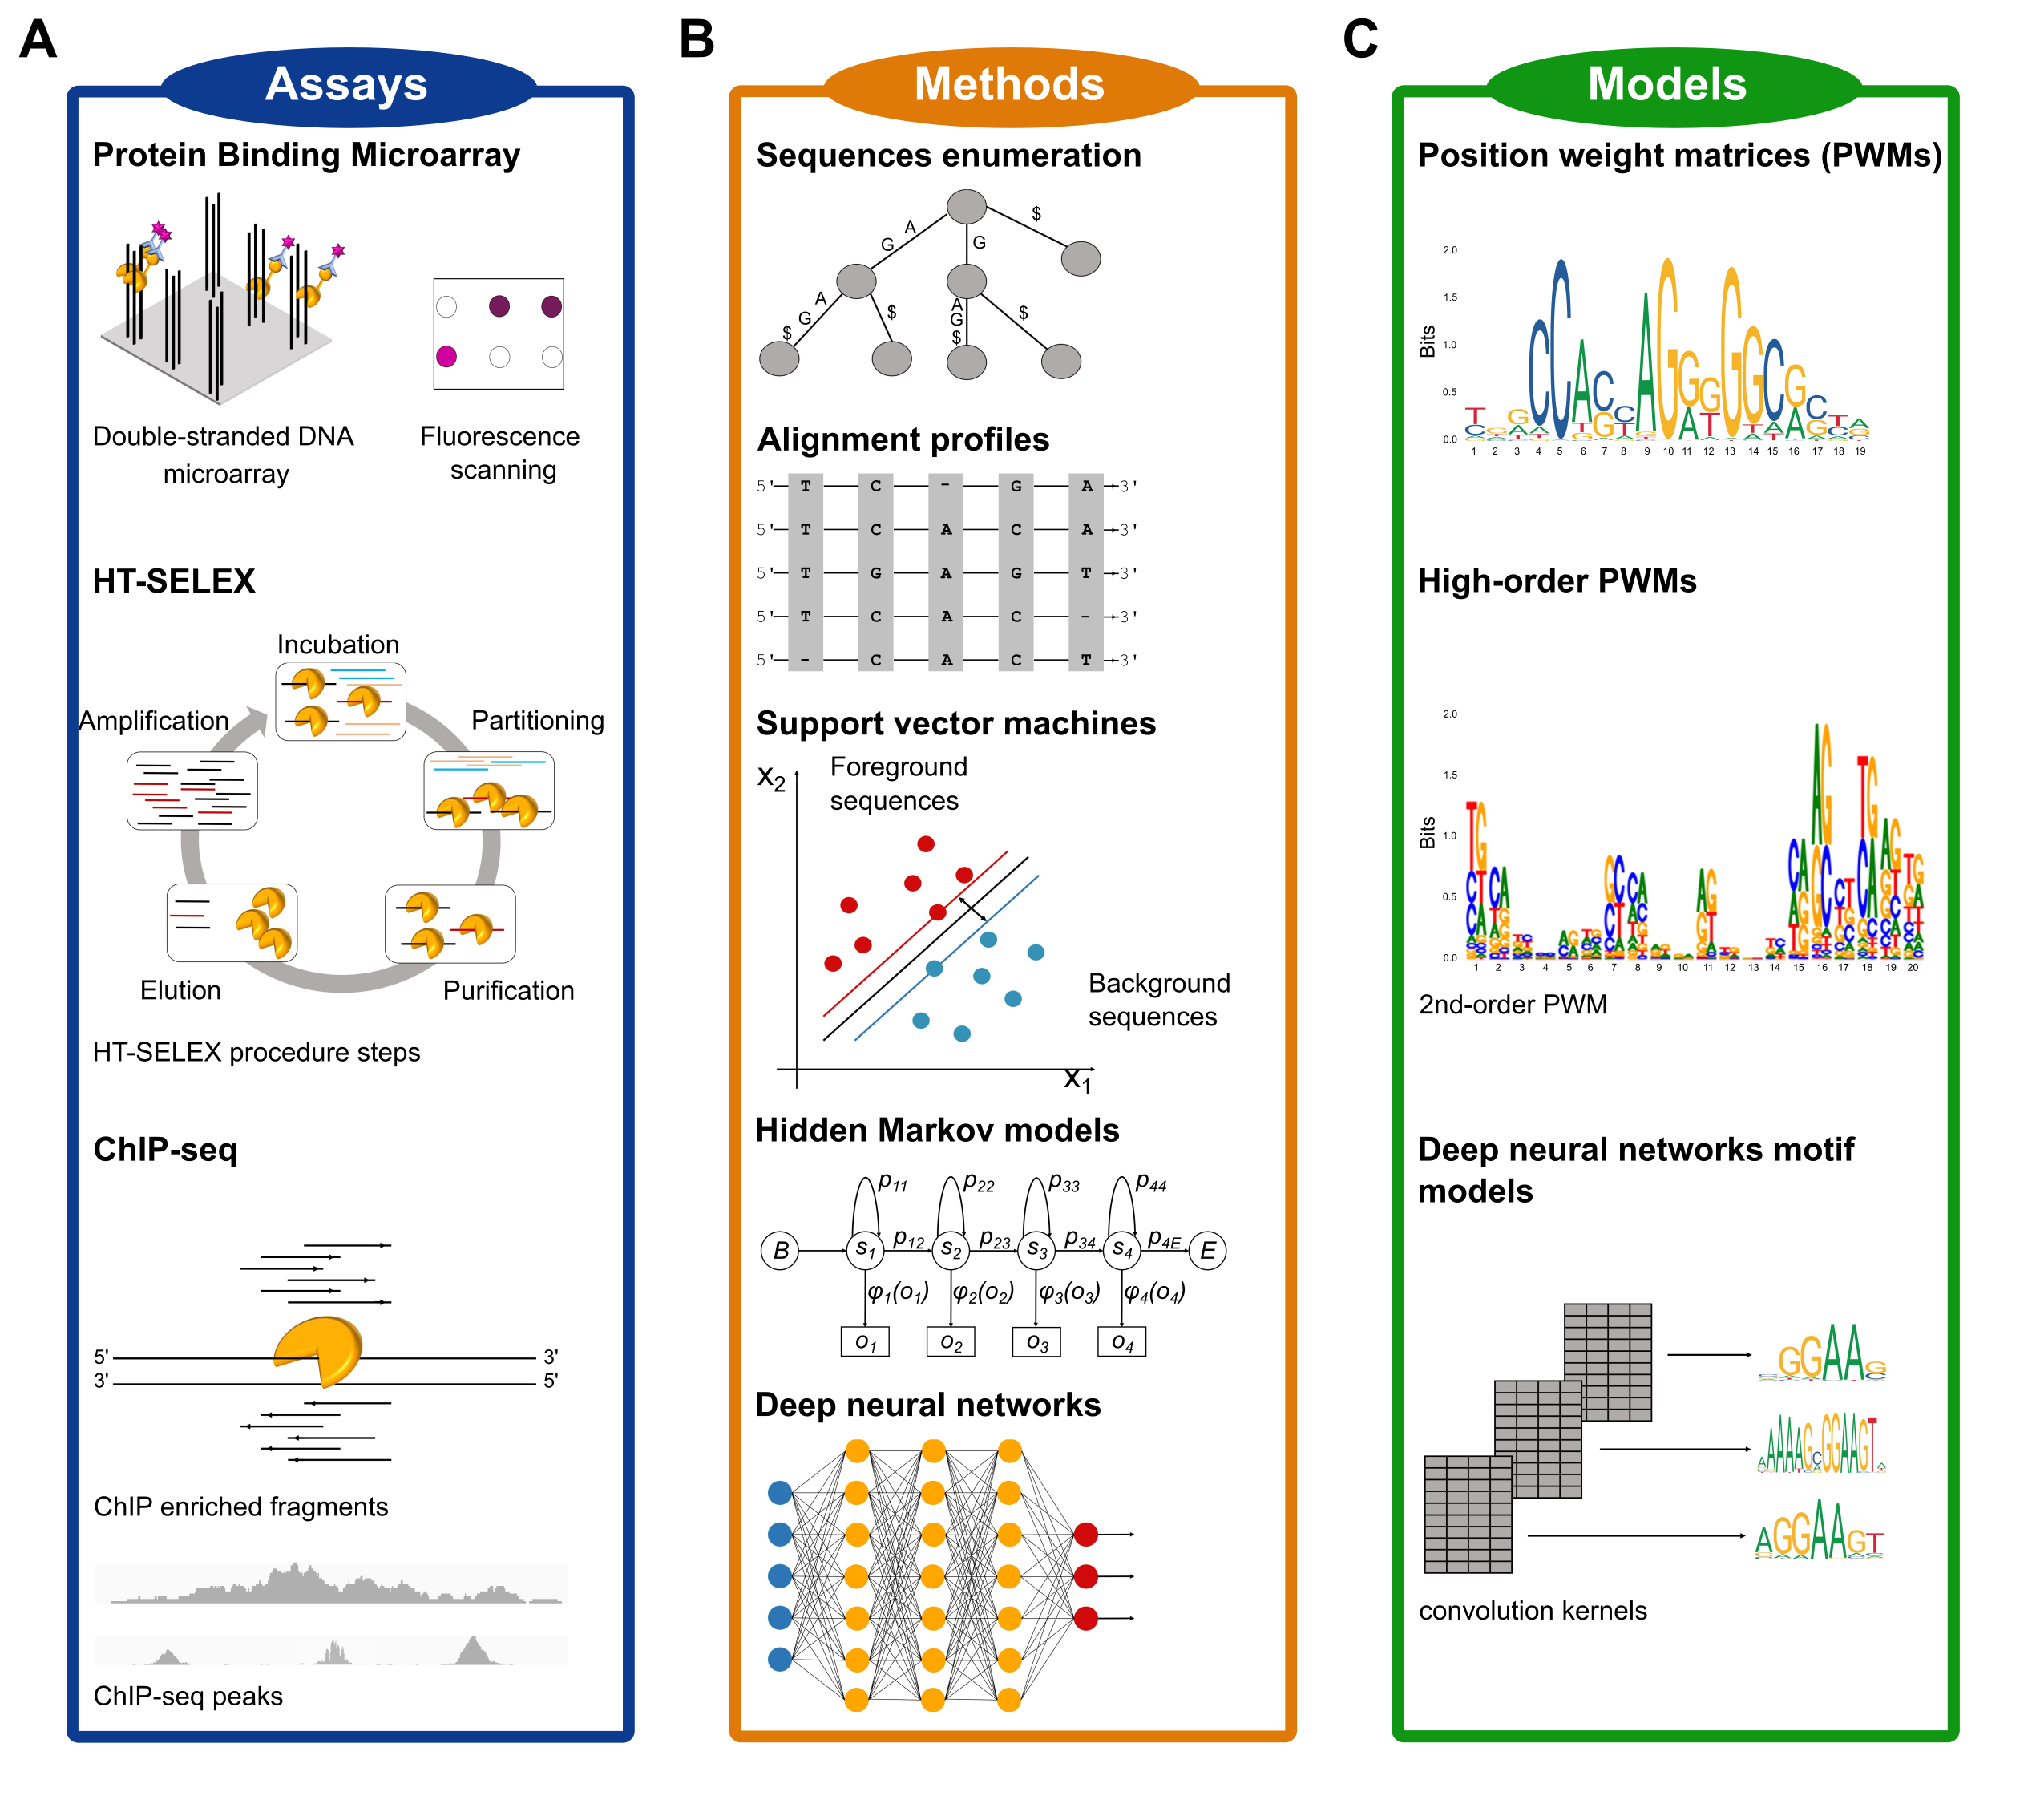
\includegraphics[width=\textwidth]{figures/md.png}
	\caption[Experimental and computational methods to discover TFBS and popular models to represent binding site motifs]{\textbf{Experimental and computational methods to discover TFBS and popular models to represent binding site motifs.} Protein binding microarray (PBM), HT-SELEX and ChIP-seq have become the most popular assays to determine TF binding preferences and identify their target sites (TFBS) in recent years. Computational motif discovery methods can be grouped into five classes, based on the algorithms employed to discover TFBS: enumerative, alignment-based, probabilistic graphical model-based, SVM-based and DNN-based methods. TFBS sequences prioritized by motif discovery algorithms are encoded in computational models representing the binding preferences of the investigated TFs.}
	\label{fig:motif_discovery}
\end{figure}

% ---- Experimental methods to discover Transcription Factor Binding Sites
\subsection{Experimental methods to discover Transcription Factor Binding Sites}
Over the past few decades, different techniques have been introduced to experimentally identify and evaluate TF binding sites along with their binding preferences \citep{jolma2011methods} (\textbf{Figure \ref{fig:motif_discovery}} and \textbf{Table \ref{tab:experimental-assays-tfs}}). Initial investigations into TF binding primarily concentrated on gene promoters \citep{stormo2000dna} and employed \emph{in vitro} methods, including the Electro-Mobility Shift Assay (EMSA) \citep{garner1981gel} and DNase footprinting \citep{galas1978dnaase}. EMSA leverages the properties of non-denatured polyacrylamide gel to separate DNA sequences into bound and unbound fractions. DNase footprinting integrates EMSA with DNase I cleavage, identifying protected regions (footprints) due to the presence of the bound TF. Typically, these assays generate datasets comprising a few hundred bound sequences, providing a constrained view of the TFs' binding landscape. Additionally, technical limitations in EMSA and DNase footprinting may introduce inaccuracies in the reported sequences and binding preferences \citep{jolma2011methods}. The advent of Next-Generation Sequencing (NGS) technologies has transformed the exploration of TFBS identification, prompting researchers to devise approaches that harness the capabilities of massively parallel sequencing (\textbf{Figure \ref{fig:motif_discovery}}). These methods offer two major advantages: (i) they operate without requiring prior knowledge of the binding site sequence \citep{jolma2011methods, zia2012towards} and (ii) generate datasets comprising thousands of bound sequences, enabling a more comprehensive characterization of TF binding preferences \citep{stormo2010determining}. Protein binding microarrays (PBMs) \citep{berger2006compact,berger2009universal} recover short TFBS sequences ($\sim$10 base pairs) and assess TF binding preferences in vitro. In PBMs, a labeled TF is applied to a glass slide containing numerous spots, each filled with short, immobilized DNA sequences. Subsequently, the labeled TFs are incubated with fluorescent antibodies targeting the label, followed by washing to eliminate weakly bound factors. The fluorescence and DNA sequence enrichment are then utilized to quantify TF-DNA binding strength and capture the bound sequences. Generally, the recovered sequences lack nucleotides flanking the investigated binding sites, yielding high-resolution datasets. However, as the number of possible sequences grows with the target length, PBMs can assess only a limited number of target sequences \citep{jolma2011methods, zia2012towards}. PBM analysis is typically restricted to binding sites $\sim$10–12 bp long. HT-SELEX, a widely employed \emph{in vitro} technique, seamlessly integrates SELEX with high-throughput sequencing \citep{jolma2011methods,jolma2010multiplexed}. This method involves releasing a TF onto a pool of randomized DNA sequences, allowing the factor to selectively pick its target sites. Subsequently, TF–DNA complexes are isolated from unbound sequences through affinity capture, followed by polymerase chain reaction (PCR) amplification and sequencing. The resulting DNA library, enriched in binding sites for the studied TF, serves as the initial pool for another SELEX run \citep{jolma2011methods,jolma2010multiplexed}. Notably, SELEX does not necessitate prior knowledge of the target sites for the investigated factor \citep{jolma2013dna}. As the SELEX reaction is typically conducted in a liquid phase, free from physical constraints, the sequence space covered by HT-SELEX often surpasses that of PBMs. Additionally, through the integration of sequencing with DNA barcode indexing, HT-SELEX enables the parallel analysis of hundreds of TFs. It yields datasets comprising thousands of high-resolution bound sequences, letting only a few nucleotides surrounding the binding sites. However, since the starting DNA library consists of randomized sequences, HT-SELEX cannot pinpoint the genomic binding locations of the investigated factor. The advent of chromatin immunoprecipitation (ChIP) technologies \citep{collas2008chop} has revolutionized the study of TFBS binding, allowing for the genome-wide identification of regions bound by TFs \emph{in vivo}. In the ChIP method, TF–DNA complexes undergo cross-linking using formaldehyde. The DNA is then fragmented into $\sim$100–1000 bp long fragments and subsequently immunoprecipitated using antibodies specific to the investigated TF. To recover the bound sequences, the cross-links are reversed. The resulting fragments can be amplified through either microarray hybridization (ChIP-on-Chip \citep{collas2008chop,pillai2015chip}) or sequencing (ChIP-seq \citep{johnson2007genome,mardis2007chip}). To locate binding regions, the recovered DNA fragments are mapped onto the genome. After mapping ChIP-seq reads, peak calling algorithms \citep{thomas2017features,guo2012high,zhang2008model} are employed to predict the genomic binding locations of the investigated factor. These algorithms identify genomic regions with higher enrichment in mapped DNA probes compared to a control experiment and designate those regions as binding locations or peaks \citep{pepke2009computation}. ChIP methods yield large datasets containing thousands of genomic regions, ranging from a few hundred to thousands of nucleotides, allowing the identification of potential TFBS for the studied factor. Despite ChIP technologies, especially ChIP-seq, being considered the current 'golden standard,' they have some limitations. ChIP can detect indirect binding, identifying other TFBS not belonging to the investigated factor \citep{worsley2014non}. ChIP-seq peaks may be false positives, arising from poor antibody quality \citep{pickrell2011false}. Finally, ChIP-seq returns low-resolution datasets, including several nucleotides flanking the target TFBS. To address the latter issue, ChIP-exo \citep{rhee2011comprehensive} utilizes lambda exonuclease to trim ChIP sequences, removing some of the nucleotides flanking the target sites. Alternatively, experimental assays targeting open chromatin regions, such as ATAC-seq \citep{buenrostro2013transposition} or DNase-seq \citep{john2011chromatin}, can be employed to recover \emph{in vivo} genomic locations likely to contain TFBS, as most TFs bind their target sequences in open chromatin regions. ATAC-seq and DNase-seq are generally used when the factors binding the target regions are not known. In summary, the current high-throughput \emph{in vivo} and \emph{in vitro} assays generate datasets comprising thousands of sequences potentially containing various possible binding configurations of TFBS, thereby enabling more comprehensive characterizations of TFs binding landscapes.

% - table: In vivo and in vitro experimental assays to identify and validate transcription factor binding sites
\begin{table}[]
    \centering
    \resizebox{\textwidth}{!}{%
    \begin{tabular}{|l|l|l|l|l|l|l|}
        \hline
        \textbf{Experimental assay}                                            & \textbf{Description}                                                                                                                                                                                                                                                                                                                                                 & \textbf{Output}                                                                                                         & \textbf{\begin{tabular}[c]{@{}l@{}}\emph{De novo} motif \\ discovery \\ capability\end{tabular}}                                 & \textbf{Type} & \textbf{\begin{tabular}[c]{@{}l@{}}Identification of \\ genomic binding \\ locations\end{tabular}} & \textbf{Throughput} \\ \hline
        Competition EMSA                                                       & \begin{tabular}[c]{@{}l@{}}Bound DNA sequences are identified \\ by observing changes in the electrophoretic \\ migration of DNA sequences through \\ non-denatured polyacrylamide gel\end{tabular}                                                                                                                                                                  & Bound DNA sequences                                                                                                     & \begin{tabular}[c]{@{}l@{}}No. Used to validate \\ known binding sites\end{tabular}                                       & \emph{in vitro}      & No                                                                                                 & Low                 \\ \hline
        DNase footprinting                                                     & \begin{tabular}[c]{@{}l@{}}Pools of DNA sequences are incubated with \\ the TF of interest; then, the DNA is degraded \\ using DNase I. The unbound fragments are \\ cut in all positions, while the bound DNA is \\ protected by the TF\end{tabular}                                                                                                                & Bound DNA sequences                                                                                                     & \begin{tabular}[c]{@{}l@{}}No. Used to validate \\ known binding sites\end{tabular}                                       & \emph{in vitro}      & No                                                                                                 & Low                 \\ \hline
        \begin{tabular}[c]{@{}l@{}}Protein Binding \\ Microarrays\end{tabular} & \begin{tabular}[c]{@{}l@{}}Arrays of $\sim$40 000 spots with short, immobilized \\ DNA sequences are incubated with a tagged TF, \\ and then washed to remove weakly bound \\ proteins. The bound sequences are identified \\ through fluorescence-based detection \& Continuous \\ values describing fluorescence intensity on each array \\ spot\end{tabular}            & \begin{tabular}[c]{@{}l@{}}Continuous values \\ describing fluorescence \\ intensity on each array \\ spot\end{tabular} & \begin{tabular}[c]{@{}l@{}}Yes. Limited to short \\ motifs\end{tabular}                                                   & \emph{in vitro}      & No                                                                                                 & High                \\ \hline
        HT-SELEX                                                               & \begin{tabular}[c]{@{}l@{}}The TF is added to a pool of randomized DNA \\ fragments. The bound sequences are selected and \\ constitute the starting pool for the next experimental \\ round. The procedure is repeated for several rounds. \\ Sequencing is employed to recover the sequence of \\ the bound DNA fragments\end{tabular}                             & DNA sequences                                                                                                           & Yes                                                                                                                       & \emph{in vitro}      & No                                                                                                 & High                \\ \hline
        \begin{tabular}[c]{@{}l@{}}ChIP-based \\ technologies\end{tabular}     & \begin{tabular}[c]{@{}l@{}}TF–DNA complexes are cross-linked with \\ formaldehyde and immunoprecipitated \\ employing TF-specific antibodies. The bound \\ sequences are then prioritized employing qPCR \\ microarrays (ChIP-on-Chip) or through sequencing \\ (ChIP-seq). ChIP-exo integrates exonuclease \\ treatment to enhance sequence resolution\end{tabular} & \begin{tabular}[c]{@{}l@{}}Genomic binding \\ location coordinates\end{tabular}                                         & \begin{tabular}[c]{@{}l@{}}Yes. Limited by the \\ inability to distinguish \\ direct and indirect \\ binding\end{tabular} & \emph{in vivo}       & Yes                                                                                                & Low                 \\ \hline
    \end{tabular}%
    }
    \caption[\emph{In vivo} and \emph{in vitro} experimental assays to identify and validate transcription factor binding sites]{\textbf{\emph{In vivo} and \emph{in vitro} experimental assays to identify and validate transcription factor binding sites.} Traditional techniques like EMSA or DNase footprinting are employed for validating established TFBS, whereas modern methods such as PBMs, HT-SELEX, and ChIP-based approaches are favored for uncovering new binding sites. Among these, ChIP-based assays stand out as the sole methods capable of retrieving the genomic locations where TFs bind. The "throughput" designation denotes the number of samples each method can process simultaneously (high: hundreds of samples; low: a few samples) (Adapted from \cite{tognon2023survey}).}
    \label{tab:experimental-assays-tfs}
\end{table}

% ---- Computational methods and models to discover and represent Transcription Factor Binding Sites
\subsection{Computational methods and models to discover and represent Transcription Factor Binding Sites}
As described in the previous section, experimental assays recover large binding site sequence datasets. However, the reported sequences often include unbound sequences and contain additional nucleotides flanking the target sites. These limitations add a layer of complexity and make manual analyses and curations challenging and often unfeasible. Motif discovery algorithms address this challenges, by providing a computational framework to analyse the datasets produced by experimental assays. Motif discovery algorithms discover potential binding sites in the analyzed sequence datasets and construct computational models representing TFBS. The problem of TFBS motif discovery can be formalized as follows. Given a set of positive DNA sequences $S$, obtained from an experimental assay targeting a specific TF, and a set of negative sequences $B$, the objective is to identify one or more recurrent, short, and similar subsequences in $S$ that maximize the discriminatory power between $S$ and $B$ \citep{tognon2023survey}. These identified subsequences are referred to as patterns or motifs and are likely to be bound by the investigated TF. The negative set $B$ may consist of randomly generated or carefully selected genomic sequences with similar nucleotide content and length to those in $S$. The patterns identified are then employed to construct and train a computational model $M$ (motif model) that represents the discovered motif. These models can then be employed to identify potential new binding sites and predict the strength of the TF–DNA binding when presented with a new set of sequences. Motif discovery can be viewed as either a classification or a regression problem, depending on the type of data used for training \citep{tognon2023survey}. Datasets from experimental assays, such as ChIP-seq or HT-SELEX, offer hundreds or thousands of sequences containing binding sites, transforming motif discovery into a classification problem. In this scenario, the objective is to differentiate between bound and unbound sites in the input sequences and train the motif model with the identified binding sites. On the other hand, datasets from other experimental technologies like PBMs provide relative binding strength for large sets of sequences of equal length. In this case, rather than distinguishing between bound and unbound sequences, $M$ learns the relative binding affinities associated with each target site in the input dataset, making motif discovery a regression problem. In both settings, the ultimate goal is to derive a computational model $M$ that characterizes the recovered TFBS and can predict new binding events, along with their affinity, in sequences not used during model training. Motif discovery algorithms can be classified into enumerative, alignment-based, probabilistic graphical models, support vector machine (SVM)-based, and deep neural network-based methods (\textbf{Figure \ref{fig:motif_discovery}} and \textbf{Appendix \ref{section:algorithms-table-appendix}}). Alternative approaches for identifying TFBS motifs in genomic sequences involve phylogenetic footprinting \citep{mccue2001phylogenetic,blanchette2002discovery}. The fundamental principle of phylogenetic footprinting posits that functional elements, such as TFBS, are more likely to be conserved across evolutionarily related species, while non-functional elements are more susceptible to mutations. Despite being one of the earliest techniques suggested for TFBS identification, phylogenetic footprinting remains widely used for assessing TFBS conservation across different organisms \citep{balazadeh2011ors1, xu2012cis,katara2012phylogenetic}. In a recent study \citep{glenwinkel2014targetortho}, the authors proposed a novel method that employs phylogenetic footprinting to discover TFBS. Before delving into the algorithms, we provide an overview about the models used to describe TFBS motifs. The prevalent models for representing TFBS include consensus sequences \citep{day1992critical}, PWMs \citep{stormo2000dna,stormo2013modeling}, high-order PWMs \citep{siddharthan2010dinucleotide,korhonen2017fast}, SVM-based \citep{gorkin2012integration}, and deep neural network-based \citep{he2021survey} models. Consensus sequences succinctly characterize identified TFBS by indicating the most frequently observed nucleotide at each motif position within a prioritized sequence set. While TFBS possess conserved positions intolerant to mutations \citep{li2015human}, other TFBS locations admit alternative nucleotides. Degenerate consensus accommodates ambiguous motif positions using IUPAC symbols. However, consensus sequences are unable to capture the contribution of each nucleotide at every motif position to TF–DNA binding. PWMs address this limitation by offering an additive model that considers the contribution of each motif position to the binding site. PWMs construct an ungapped alignment between candidate motif sequences and tally the frequency of each nucleotide at each position. The statistical significance of PWMs is often assessed using relative entropy (RE) \citep{stormo1998information}. RE measures the difference between computed nucleotide frequencies and those derived from aligning random sequences. PWMs are visualized as logos \citep{schneider1990sequence}, where the height of each nucleotide is proportional to its RE. Despite their widespread success, PWMs still assume independence between motif positions. To address this limitation, probabilistic graphical models model dependencies between motif nucleotides. These models encompass high-order PWMs such as dinucleotide weight matrices (DWMs), Bayesian networks (BNs), Markov models (MMs), or hidden Markov models (HMMs) \citep{siddharthan2010dinucleotide,korhonen2017fast,barash2003modeling,siebert2016bayesian}. DWMs and high-order PWMs are commonly visualized as logos with $q$-mers replacing single nucleotides, where $q$ represents the dependency order between adjacent nucleotides. Notably, probabilistic graphical models can accommodate variable spacing between half-sites of two box motifs \citep{mathelier2013next}. However, the number of model parameters and its complexity increase exponentially with $q$, often leading to models overfitting the input dataset. SVM-based models use a SVM kernel to learn the binding site structure from the input sequence dataset. TFBS is represented either by a list of $k$-mers with associated weights or support vectors used to discriminate between bound and unbound sequences, depending on the employed kernel \citep{boeva2016analysis}. In the former case, the weights reflect the $k$-mer contribution to the motif sequence. SVM-based models can accommodate variable spacing between the half-sites of two box motifs, similar to probabilistic graphical models. Importantly, $k$-mers indirectly capture $k$-th order dependencies between neighboring nucleotides. However, simple SVM-based models are restricted to considering short ($\sim$10 bp) and cannot effectively represent longer motifs. Gapped $k$-mers \citep{ghandi2014robust} addressed this limitation by handling longer TFBS and accounting for sequence degeneration in non-informative motif positions. To visualize the discovered motifs, SVM-based models are often simplified to PWMs by aligning the informative $k$-mers. Deep neural network (DNN)-based models integrate the diverse, complex, and hierarchical patterns governing TF–DNA binding events in input nucleotide sequences. Despite their accuracy and power, a major limitation of DNN-based models is their 'black box' nature \citep{park2020enhancing}. Many frameworks visualize the discovered motifs as PWMs, computed by aligning the sequences activating the convolutional kernels of the DNN \citep{koo2020deep}. However, DNNs often learn distributed representations where multiple neurons cooperate to describe single patterns. Consequently, motifs learned by single kernels and the resulting PWMs tend to be redundant with each other. DeepLIFT \citep{shrikumar2017learning} introduced a method to assign importance scores to the kernels. By comparing the activation of each neuron to a reference value, DeepLIFT identifies which kernels contribute most to defining the TFBS, thereby reducing motif redundancy. TF-MoDISco \citep{avsec2021base} extended this idea by clustering and aggregating the discovered motifs, using the importance scores assigned to the kernels. However, generating interpretable models without sacrificing some information learned by the DNN remains an open challenge.

% --- Enumerative methods
\subsubsection{Enumerative methods}
Enumerative algorithms for motif discovery (\textbf{Figure \ref{fig:motif_discovery}}) assume that motifs are patterns overrepresented in the input dataset $S$, compared to a background set of genomic sequences
$B$⁠. Enumerative algorithms typically assume that the motif length $|M|$ is known \emph{a priori}. The fundamental idea involves collecting the approximate occurrences of all potential $4^{k}$ $k$-mers within the sequences of $S$ and evaluating the statistical significance by comparing the observed matches in $S$
with those expected from a background model. Subsequently, a PWM is derived by constructing an ungapped alignment from the statistically significant $k$-mers. However, the exhaustive search for approximate occurrences of all $k$-mers quickly becomes impractical, particularly for larger $S$. Early methods incorporated heuristics to address this challenge, such as limiting the search to patterns occurring at least once in each sequence $s \in S$ \citep{li1999finding} or restricting mismatching locations to specific motif positions \citep{califano2000splash}. Nonetheless, allowing mismatches at any motif position is crucial. To address this, Weeder \citep{pavesi2001algorithm,pavesi2004weeder} and SMILE \citep{marsan2000algorithms} proposed using suffix trees (STs) \citep{weiner1973linear} to efficiently navigate the entire motif search space. Leveraging the indexing capabilities of STs enables the algorithms to conduct approximate pattern matching without imposing restrictions on mismatching positions. This approach ensures high accuracy in motif discovery while mitigating computational costs. For assessing the statistical significance of motif candidates, SMILE and Weeder compare motif frequencies in $S$ with those in a set of randomly generated genomic sequences or the promoters of the same organism, respectively (\textbf{Appendix \ref{subsection:enumerative-methods-appendix}}). However, these strategies often prove computationally demanding and lack scalability when applied to the extensive datasets produced by PBMs, HT-SELEX, or ChIP assays \citep{liu2018algorithmic}. As a result, more efficient methods tailored for large datasets have been proposed. MDscan \citep{liu2002algorithm} and Amadeus \citep{linhart2008transcription} employ word enumeration to identify potential motifs in sequence datasets (\textbf{Appendix \ref{subsection:enumerative-methods-appendix}}). MDscan leverages the shape of ChIP peaks to identify non-redundant patterns that are abundant in the most enriched sequences, employing a third-order Markov background model to gauge the statistical significance of motifs. Amadeus assesses all $k$-mers in $S$ and organizes similar patterns into lists, which are then grouped into motifs and statistically evaluated using a hypergeometric test. However, word enumeration may still be computationally demanding. In response to this, DREME \citep{bailey2011dreme} introduced the use of regular expressions to approximate motif frequencies in $S$ and $B$⁠. To evaluate motifs' statistical significance, DREME employs Fisher’s exact test, comparing the number of motif occurrences detected in $S$
and $B$. Nevertheless, regular expressions can be computationally expensive for large $S$, potentially leading to false positives or missing motifs. Trawler \citep{ettwiller2007trawler}, HOMER \citep{heinz2010simple}, and STREME \citep{bailey2021streme} reintroduced STs and proposed different optimizations to enhance scalability for large datasets (\textbf{Appendix \ref{subsection:enumerative-methods-appendix}}). Trawler and HOMER improved the statistical significance assessment step using $z$-scores derived from the normal approximation to the binomial distribution and the hypergeometric distribution, respectively. In contrast, STREME reduces the motif search space by initially identifying overrepresented seed words of different lengths on the ST. Subsequently, STREME counts the number of approximate matches for the most significant words on the ST. By identifying seeds of varying lengths, STREME can discover motifs of different lengths in a single tree visit.

% --- Alignment-based methods
\subsubsection{Alignment-based methods}
Alignment-based motif discovery algorithms generate alignment profiles to characterize motifs' binding preferences (\textbf{Figure \ref{fig:motif_discovery}}), avoiding the exhaustive enumeration of $k$-mers. In this approach, an alignment is constructed by selecting motif candidate sequences from the input dataset $S$ and evaluating the resulting profile using various metrics, such as nucleotide conservation, information content, or the statistical significance of the profile. The motif's statistical significance is assessed by computing the probability of obtaining the same alignment from a background dataset $B$ or random sequences. Typically, alignment-based motif discovery algorithms assume that the motif length $|M|$ is known in advance. Formally, for alignment-based algorithms, motif discovery can be viewed as a combinatorial problem. Given $|M| = k$, the goal is to identify the optimal alignment profile by combining $k$-mers from $S$, according to a scoring criterion. The best alignments are then used to generate the corresponding PWMs. Most alignment-based algorithms assume that each sequence in $S$ contains either zero or one binding site, resulting in $(\sum_{s \in S}{|s| - |M| + 1})^{|S|}$ possible profiles built combining $k$-mers in all possible ways. However, enumerating all potential solutions is computationally impractical, even for small datasets. As a solution, alignment-based algorithms employ heuristics such as greedy strategies \citep{hertz1999identifying}, expectation–maximization (EM) \citep{bailey1994fitting}, stochastic methods (e.g., Gibbs sampling) \citep{lawrence1993detecting}, or genetic algorithms \citep{lee2018comprehensive} (\textbf{Appendix \ref{subsection:alignment-methods-appendix}}). CONSENSUS \citep{hertz1999identifying} introduced a greedy strategy to incrementally construct alignment profiles. It initially solves the problem for two sequences and gradually expands by incorporating the remaining sequences one by one. CONSENSUS stores the best partial alignments with the hope of identifying the highest-scoring profiles. However, in cases where motifs lack conservation, CONSENSUS might discard potentially highest-scoring solutions. The MEME algorithm \citep{bailey1994fitting,bailey1995value,bailey2006meme} adopts a distinct strategy based on Expectation-Maximization (EM). It iteratively refines an initial profile by substituting some $k$-mers in the profile with others more likely to yield improved solutions. MEME evaluates the fit of each $k$-mer in the dataset to the current profile, bypassing the need for a background model. MEME identifies motifs occurring multiple times in each sequence and calculates their statistical significance without relying on TFBS conservation. However, the algorithm may prematurely converge to local maxima, and convergence heavily relies on the initial conditions of the algorithm. In contrast to MEME, Gibbs sampling \citep{lawrence1990expectation} employs a stochastic approach to add $k$-mers to the alignment rather than a deterministic one based on profile fit. Gibbs sampling replaces $k$-mers in the profile with others selected with a probability proportional to their likelihood score (\textbf{Appendix \ref{subsection:alignment-methods-appendix}}). The stochastic nature of the Gibbs sampling algorithm reduces the likelihood of converging to local maxima, but achieving reliable results may necessitate multiple runs. Despite this, several methods employing Gibbs sampling and its extensions have been proposed \citep{neuwald1995gibbs,hughes2000computational,workman1999ann,liu2000bioprospector,thijs2001higher,frith2004finding,frith2008discovering} (\textbf{Appendix \ref{subsection:alignment-methods-appendix}}). Genetic algorithms offer an alternative approach to address the limitations of EM and stochastic methods. GADEM \citep{li2009gadem} combines EM local search with genetic algorithms to refine profiles, preventing convergence to local maxima and mitigating the stochastic nature of Gibbs sampling. However, due to their computational complexity, genetic algorithms pose challenges when analyzing datasets containing thousands of sequences. Since the solution space for algorithms using alignment profiles grows exponentially with the size of $S$, and even with the use of heuristics, analyzing thousands of sequences becomes computationally impractical \citep{zambelli2013motif}. Therefore, researchers have directed their efforts toward developing algorithms specifically tailored to analyze the large datasets produced by high-throughput assays (\textbf{Appendix \ref{subsection:alignment-methods-appendix}}). MEME-ChIP \citep{machanick2011meme} and STEME \citep{reid2011steme} enhance the MEME algorithm for ChIP datasets. While MEME-ChIP focuses the analysis on a random subset of sequences, STEME accelerates EM steps by indexing the sequences in a suffix tree. However, using random subsets of $S$ may lead to missing critical motif instances, and constructing a suffix tree from thousands of sequences may be computationally demanding. ChIPMunk \citep{kulakovskiy2010deep} introduces a greedy profile optimization, similar to EM, designed to discover motifs in large ChIP-seq datasets, while accounting for ChIP peak shapes. XXmotif \citep{hartmann2013p} and ProSampler \citep{li2019prosampler} propose methods that combine enumerative motif discovery with iterative and stochastic profile refinement, respectively.

% --- Probabilistic graphical model-based methods
\subsubsection{Probabilistic graphical model-based methods}
Including dependencies between nucleotides within TFBS has been a topic of discussion within the community \citep{tomovic2007position,morris2011jury,zhao2011quantitative}. Some studies have demonstrated the existence of dependencies between both neighboring and non-neighboring nucleotides in TFBS \citep{slattery2014absence,rohs2010origins}. Enumerative and alignment-based algorithms typically represent motifs as PWMs, which do not inherently incorporate dependencies between binding site positions. Although PWMs can be extended to account for di- or trinucleotide frequencies (high-order PWMs), such as DWMs \citep{siddharthan2010dinucleotide}, methods like Dimont \citep{grau2013general} and diChIPMunk \citep{kulakovskiy2013binding} have proposed extensions to alignment-based approaches, representing motifs as DWMs to capture dependencies, albeit primarily focusing on neighboring nucleotides (\textbf{Appendix \ref{subsection:probabilistic-methods-appendix}}). Probabilistic graphical models (\textbf{Figure \ref{fig:motif_discovery}}), including Bayesian Networks (BNs), Markov Models (MMs), or Hidden Markov Models (HMMs), offer robust frameworks for capturing dependencies between nucleotides within TFBS. A study \citep{barash2003modeling} suggested using BNs trained through Expectation-Maximization (EM) to model TFBS, capturing dependencies between both neighboring and non-neighboring positions. However, this method assumes a consistent order of dependence throughout the entire motif. Another approach, Variable Order Bayesian Networks (VOBNs) \citep{ben2005identification}, utilizes BNs considering variable orders of dependencies between positions. Nonetheless, training BNs can be computationally challenging when dealing with thousands of sequences, and these models may be prone to overfitting even when trained on hundreds of sequences. MMs and HMMs offer more efficient and scalable frameworks compared to BNs for incorporating dependencies between motif positions. Consequently, recent algorithmic developments have leaned towards models like TFFMs \citep{mathelier2013next} and Discrover \citep{maaskola2014binding}, proposing HMM-based models learning dinucleotide dependencies between neighboring motif positions in extensive sequence datasets. TFFMs, for instance, also learn characteristics of the sequences flanking the TFBS. MMs have been extended to capture various orders of dependencies between neighboring nucleotides, as demonstrated in a study \citep{eggeling2014value} focusing on discovering CTCF \citep{bell1999protein} motifs using variable-order MMs. Similarly, Slim \citep{keilwagen2015varying} has extended MMs to capture dependencies between non-neighboring nucleotides. However, MMs and HMMs typically only capture low-order dependencies. In contrast, BaMMotif \citep{siebert2016bayesian,ge2021bayesian} has proposed a motif discovery algorithm using a Bayesian approach to efficiently train Markov models with dependencies up to the fifth order, even on large datasets comprising thousands of sequences.

% --- SVM-based methods
\subsubsection{SVM-based methods}
Support Vector Machines (SVMs) \citep{boser1992training} have proven successful in various computational biology problems, including the discovery of transcription factor binding site (TFBS) motifs (\textbf{Figure \ref{fig:motif_discovery}}). This is achieved by decomposing bound sequences (foreground dataset $S$) and unbound sequences (background dataset $B$) into $k$-mers, using their frequencies as features to train a sequence similarity kernel \citep{ben2008support}. Typically, each $k$-mer is assigned a weight proportional to its contribution to defining positive or negative training sets or its likelihood of being a motif candidate. While earlier methods were designed for protein sequence homology \citep{leslie2001spectrum,eskin2002mismatch,kuang2005profile}, recent SVM-based algorithms are designed specifically for TFBS motif discovery. SVMs demonstrate efficiency in analyzing datasets comprising thousands of sequences. Kmer-SVM \citep{lee2011discriminative,fletez2013kmer} proposed a method for discovering TFBS motifs in sequence datasets employing the spectrum kernel. By counting exact matches for all contiguous $k$-mers in $S$ and $B$, Kmer-SVM constructs the $k$-mers feature space (\textbf{Appendix \ref{subsection:svm-methods-appendix}}). The introduction of mismatch \citep{kuang2005profile} and wildcard \citep{leslie2003fast} kernels allowed counting $k$-mer frequencies while allowing a fixed number of mismatching positions for each $k$-mer. This concept was later expanded to enable less restrictive $k$-mer frequency estimation, providing flexibility in motif structure without compromising scalability on large datasets. Agius and colleagues \citep{agius2010high} further extended this concept by developing the di-mismatch kernel, a first-order Markov mismatch kernel based on the dinucleotide alphabet. This kernel addresses sequence variability and considers dependencies between neighboring nucleotides (\textbf{Appendix \ref{subsection:svm-methods-appendix}}). To ensure scalability on large datasets, a small $k$ ($k=4$) is employed, which enables the discovery of short motifs. However, TFBS lengths typically range between 6 to 20 base pairs, making it challenging to fully characterize longer motifs with short $k$-mers. Additionally, increasing $k$ often leads to sparse feature vectors overfitting to the training dataset. Gapped k-mers \citep{ghandi2014robust} proposed representing longer motifs as $k$-mers with gaps in non-informative or degenerate TFBS positions, accounting for motif variability in sequence and length. Gkm-SVM \citep{ghandi2014enhanced,ghandi2016gkmsvm} extends Kmer-SVM to train SVM kernels employing gapped $k$-mers as features. The algorithm considers larger $k$, preventing model overfitting and reducing dependency on parameter choice. LS-GKM \citep{lee2016ls} optimizes the algorithm for scalable SVM training with gapped-$k$-mers on large-scale sequence datasets and provides various kernels for SVM training (\textbf{Appendix \ref{subsection:svm-methods-appendix}}).

% --- Deep Neural Networks-based methods
\subsubsection{Deep Neural Networks-based methods}
DNNs have gained significant popularity in computational biology \citep{talukder2021interpretation, zeng2020integrating, singh2016deepchrome, singh2019predicting, zeng2018prediction, kelley2018sequential, li2019deeptact, yin2019deephistone, manzanarez2018model} owing to their ability to discern complex patterns \citep{park2015deep} from large omics datasets \citep{zhang2019deep}. Originally designed for image classification  \citep{lecun2015deep, sainath2013improvements, vu2017use}, Convolutional Neural Networks (CNNs) \citep{lecun2015deep} have proven successful in analyzing \emph{in vivo} TF–DNA interactions \citep{alipanahi2015predicting, zhou2015predicting, kelley2016basset, zeng2016convolutional} (\textbf{Figure \ref{fig:motif_discovery}}). By applying non-linear transformations to input data, CNNs learn and represent complex patterns in a high-dimensional space \citep{bengio2013representation}, simplifying classification tasks and enabling accurate prediction of TFBS in genomic sequences. Genomic sequences are often represented as 1D or 2D images with four associated channels (A, C, G, T) \citep{zeng2016convolutional}, transforming TFBS classification into a two-class image classification problem. Typically, CNN architectures for motif discovery and classification consist of sets of four layers: the convolutional layer, max-pooling layer, fully connected NN layer, and the output layer \citep{zeng2016convolutional} (\textbf{Appendix \ref{subsection:dnn-methods-appendix}}). DeepBind \citep{alipanahi2015predicting} and Basset \citep{kelley2016basset} introduced two CNN architectures for motif discovery across different datasets, including ChIP-seq, HT-SELEX, PBM, and DNase-seq (\textbf{Appendix \ref{subsection:dnn-methods-appendix}}). The motifs discovered by DeepBind and Basset are visualized as PWMs, computed by aligning and grouping sequences that activate the convolutional layer. While DeepBind and Basset have shown promising results, their performance may be constrained by the quality of training data and the significant computational resources and time required for model training. These challenges have spurred the development of novel methods like BPNet \citep{avsec2021base}, which address some of these issues by incorporating additional features into the model and using more efficient training processes. BPNet proposed a dilated CNN architecture that enables the model to learn and integrate diverse complex features without sacrificing the spatial and base resolution of the input data (\textbf{Appendix \ref{subsection:dnn-methods-appendix}}). However, TF–DNA interactions involve not only direct binding but also interactions between multiple binding subregions (long-term interactions) and nucleotides with high-order structures of TFs (short-term interactions). Long Short-Term Memory networks (LSTMs) \citep{hochreiter1997long} and Bidirectional LSTMs (BLSTMs) efficiently capture long-term and short-term dependencies in sequential signals. Given that genomic sequences can be viewed as sequential signals with long-term and short-term dependencies, LSTMs and BLSTMs are well-suited for modeling TF–DNA interactions (\textbf{Appendix \ref{subsection:dnn-methods-appendix}}). DeeperBind \citep{hassanzadeh2016deeperbind} introduced a hybrid CNN–LSTM architecture by removing the pooling layer to maintain positional information of potential motif instances. Similarly, DanQ \citep{quang2016danq} proposed a hybrid CNN–BLSTM architecture to capture the positional dynamics of genomic sequences for TFBS motif discovery. The BLSTM replaces the fully connected NN. Factornet \citep{quang2019factornet} extended DanQ's framework by incorporating additional features and employing a Siamese BLSTM architecture to enhance model training.

% ---- Transcription Factor Databases
\subsection{Transcription Factor Databases}
With the recent advancements in experimental technologies, an extensive amount of transcription factor-related data has been generated and has been stored in different databases (\textbf{Table \ref{tab:motif_databases}}). The ENCODE project \citep{encode2012integrated} stands out as a valuable resource, offering a multitude of data on functional elements within the human genome, gathered across different tissues and cell types. ENCODE stores several TF-related genomic data encompassing ChIP-seq data targeting various TFs and DNase-seq information. Similarly, Cistrome \citep{zheng2019cistrome} and GTRD \citep{kolmykov2021gtrd} contribute to the landscape by providing TF-related genomic data from different organisms and spanning various species, cell types, and tissues. GTRD, in particular, provides extensive collections of curated ChIP-seq, ChIP-exo, and ChIP-nexus datasets. HOCOMOCO \citep{kulakovskiy2013hocomoco,kulakovskiy2018hocomoco} and JASPAR \citep{sandelin2004jaspar,fornes2020jaspar} provide large collections of curated and experimentally derived TFBS motifs. These databases store Position Weight Matrices (PWMs) and Dinucleotide Weight Matrices (DWMs) obtained through the analysis of ChIP-seq and SELEX datasets. Notably, HOCOMOCO models integrate sequence datasets with evolutionary conservation and DNA shape. Similarly, Cis-BP \citep{weirauch2014determination} incorporates experimentally derived and computationally predicted PWMs from various sources, including published literature, other databases, and experimental datasets. TRANSFAC \citep{wingender1996transfac,wingender2000transfac} emerges as a comprehensive repository, collecting experimentally validated and manually curated PWMs for different TFs from diverse eukaryotic organisms. It includes data on TF-associated proteins, DNA binding domains, and regulatory elements. FactorBook \citep{pratt2022factorbook} provides computationally predicted PWMs generated by analyzing ENCODE data, coupled with TF expression data across tissues and cell types. Unibind \citep{puig2015human} collects experimentally validated and curated PWMs from different organisms. It provides insights on the structural properties and conformation of TF–DNA complexes, along with their genomic binding locations across various cell types and tissues. UniPROBE \citep{newburger2009uniprobe} stores curated PWMs for several eukaryotic TFs, generated by analyzing Protein Binding Microarray datasets. HTRIdb \citep{bovolenta2012htridb} focuses on data pertaining to TF–target gene interactions in humans. This information, derived from published literature and other databases, spans different cell types, experimental methods, and disease states. The database also provides functional annotations for the target genes. TFcancer \citep{huang2021tfcancer} collects TF–gene interactions across 33 cancer types. The database offers tools to identify TF expression alterations and elucidate their roles in biological processes and signaling pathways associated with cancer.

% - table: Transcription Factor databases
\begin{table}[!]
    \centering
    \resizebox{\columnwidth}{!}{%
        \begin{tabular}{|l|l|l|l|l|l|}
            \hline
            \textbf{Type} &
            \textbf{Name} &
            \textbf{Reference} &
            \textbf{Data type} &
            \textbf{Model Organisms} &
            \textbf{TFs} \\ \hline
            Sequence database &
            ENCODE &
            \cite{encode2012integrated} &
            \begin{tabular}[c]{@{}l@{}}ChIP-seq\\ DNase-seq\\ ATAC-seq\end{tabular} &
            \textit{\begin{tabular}[c]{@{}l@{}}C. elegans\\ D. melanogaster\\ H. sapiens\\ M. musculus\\ \hfill \end{tabular}} &
            \textgreater 1,500 \\ 
            &
            Cistrome &
            \cite{zheng2019cistrome} &
            \begin{tabular}[c]{@{}l@{}}ChIP-seq\\ DNase-seq\end{tabular} &
            \textit{\begin{tabular}[c]{@{}l@{}}H. sapiens\\ M. musculus\\ \hfill \end{tabular}} &
            1,773 (ChIP-seq) \\ 
            &
            GTRD &
            \cite{kolmykov2021gtrd} &
            \begin{tabular}[c]{@{}l@{}}ChIP-seq\\ ChIP-exo\\ ChIP-nexus\\ DNase-seq\end{tabular} &
            \textit{\begin{tabular}[c]{@{}l@{}}A. thaliana\\ C. elegans\\ D. rerio\\ D. melanogaster\\ H. sapiens\\ M. musculus\\ R. norvegicus\\ S. cerevisiae\\ S. pombe\end{tabular}} &
            \begin{tabular}[c]{@{}l@{}}3,988 (ChIP-seq)\\ 1,708 (ChIP-exo + ChIP-nexus)\end{tabular} \\ \hline
            Motif models database &
            HOCOMOCO &
            \cite{kulakovskiy2013hocomoco,kulakovskiy2018hocomoco} &
            \begin{tabular}[c]{@{}l@{}}PWMs\\ DWMs\end{tabular} &
            \textit{\begin{tabular}[c]{@{}l@{}}H.sapiens\\ M. musculus\\ \hfill\end{tabular}} &
            \begin{tabular}[c]{@{}l@{}}680 (human)\\ 453 (mouse)\end{tabular} \\ 
            &
            JASPAR &
            \cite{sandelin2004jaspar,fornes2020jaspar} &
            \begin{tabular}[c]{@{}l@{}}PWMs\\ DWMs\end{tabular} &
            \begin{tabular}[[c]{@{}l@{}}53 species\\ \hfill\end{tabular} &
            \textgreater 1,500 \\ 
            &
            Cis-BP &
            \cite{weirauch2014determination} &
            PWMs &
            \textit{\begin{tabular}[c]{@{}l@{}}A. thaliana\\ C. elegans\\ D. rerio\\ D. melanogaster\\ H. sapiens\\ M. musculus\\ N. crassa\\ R. norvegicus\\ S. cerevisiae\\ X. tropicalis\\ \hfill\end{tabular}} &
            \textgreater 5,000 \\
            &
            TRANSFAC &
            \cite{wingender1996transfac,wingender2000transfac} &
            PWMs &
            \begin{tabular}[[c]{@{}l@{}} \textgreater 300 species\\ \hfill\end{tabular} &
            \textgreater 10,000 \\ 
            &
            FactorBook &
            \cite{pratt2022factorbook} &
            PWMs &
            \textit{\begin{tabular}[c]{@{}l@{}}H. sapiens\\ M. musculus\\ \hfill\end{tabular}} &
            \begin{tabular}[c]{@{}l@{}}881 (human)\\ 49 (mouse)\end{tabular} \\ 
            &
            UniPROBE &
            \cite{newburger2009uniprobe} &
            PWMs &
            \textit{\begin{tabular}[c]{@{}l@{}}C. elegans\\ C. parvum\\ H. sapiens\\ M. musculus\\ P. falciparum\\ S. cerevisiae\\ V. harveyi\\ \hfill\end{tabular}} &
            726 \\ 
            &
            Unibind &
            \cite{puig2015human} &
            PWMs &
            \textit{\begin{tabular}[c]{@{}l@{}}A. thaliana\\ C. elegans\\ D. rerio\\ D. melanogaster\\ H. sapiens\\ M. musculus\\ R. norvegicus\\ S. cerevisiae\\ S. pombe\\ \hfill\end{tabular}} &
            841 \\ \hline
            \begin{tabular}[c]{@{}l@{}}TF-target gene interaction\\ database\end{tabular} &
            HTRIdb &
            \cite{bovolenta2012htridb} &
            \begin{tabular}[c]{@{}l@{}}TF-gene interaction\\ networks\end{tabular} &
            \textit{H. sapiens} &
            284 \\ \hline
            \begin{tabular}[c]{@{}l@{}}TF-disease association\\ database\end{tabular} &
            TFcancer &
            \cite{huang2021tfcancer} &
            TF-cancer associations &
            \textit{H. sapiens} &
            364 \\ \hline
        \end{tabular}%
    }
    \caption[Transcription Factor Databases]{\textbf{Transcription Factor Databases.} The table provides a condensed overview of the TF-related databases discussed in \textbf{Section 4.2.3}. It outlines key aspects for each database, including its primary purpose (\textbf{Type}), the variety of available data types (\textbf{Data type}), the model organisms covered by the database (\textbf{Model organisms}), and the total number of included TFs (\textbf{TFs}).}
    \label{tab:motif_databases}
\end{table}

% ---- Downstream analysis using Transcription Factor Binding Site motifs
\subsection{Downstream analysis using Transcription Factor Binding Site motifs}
The discovered motifs serve various purposes in downstream analyses, including motif comparison, motif scanning, motif enrichment analysis, and evaluating the effects of genetic variants on TF–DNA binding affinity \citep{tognon2023survey}. Motif comparison measures the similarity between the discovered motifs and annotated TFBS, facilitating the connection of known TFs to newly identified motifs \citep{gupta2007quantifying}. Tools such as Tomtom \citep{gupta2007quantifying}, STAMP \citep{mahony2007stamp}, MACRO-APE \citep{vorontsov2013jaccard}, or MoSBAT \citep{lambert2016motif} are commonly used for this task, searching annotated databases for motifs matching the input consensus sequence or inferred motif matrix. Additionally, motif comparison tools have been developed to interpret and annotate potential motifs encoded in the convolutional filters of CNN models. Motif scanning involves searching sets of genomic regions for potential occurrences of the input motif, aiming to recover potential binding locations for the investigated factor. Motif scanning algorithms assign scores to sequences using the input model (e.g., a PWM). A challenge in motif scanning is the choice of a reliable cutoff for discriminating between true and false binding events \citep{boeva2016analysis}. Several motif scanning tools are available, such as \citep{korhonen2009moods}, FIMO \citep{grant2011fimo}, PWMscan \citep{ambrosini2018pwmscan}, and the HOMER suite \citep{heinz2010simple}. Recently, MOODS has been extended to search instances of motifs modeled as high-order PWMs \citep{korhonen2017fast}. However, motif scanning algorithms generally do not consider individual- and population-specific genetic variants and haplotypes while searching for potential motif occurrences. This may result in several potential TFBS missed and missing information which could facilitate the interpretation of genetic variants impact within the cell. Motif enrichment analysis (MEA) investigates over- and underrepresented motifs in gene regulatory regions, linking investigated TFs to their functions within the cell environment. MEA involves scanning regulatory regions for motif occurrences and statistically testing motif enrichment. There are many MEA tools available, such as Clover \citep{frith2004detection}, Pscan \citep{zambelli2009pscan}, AME \citep{mcleay2010motif}, or oPOSSUM-3 \citep{kwon2012opossum} are commonly used for MEA. The HOMER suite provides MEA functionality. Haystack \citep{pinello2018haystack} proposed an integrated MEA strategy, exploring motif enrichment in cell-type-specific regions and incorporating gene expression data to assess the transcriptional activity of studied factors and their impact on regulated genes.

% ---- Evaluating genetic variants impact on Transcription Factor Binding Sites
\subsection{Evaluating genetic variants impact on Transcription Factor Binding Sites}
Genetic variants have been demonstrated to influence TF–DNA binding events \citep{de2006regulatory,wienert2015editing,weinhold2014genome}, with implications for common diseases through their association with regulatory elements \citep{maurano2012systematic}. These variants have the potential to alter the transcriptional state of the cell \citep{deplancke2016genetics}, leading to an increasing interest in developing tools to predict the impact of variants on TFBS (\textbf{Table \ref{tab:variants_tools_motif}}). TRAP \citep{thomas2011transcription} and CATO \citep{maurano2015large} employ PWMs to predict variant impact on TFBS by comparing binding affinity scores between reference and alternative sequences. TRAP repeats this process across a collection of TFBS, reporting the motif with the most significant score change. CATO, on the other hand, generates a ranked list of disrupted motifs using a logistic model trained with information content differences, TF occupancy, and phylogenetic conservation between reference and alternative sequences. However, these methods face scalability issues when analyzing thousands of SNPs. atSNP \citep{zuo2015atsnp} introduces a scalable strategy to assess the impact of thousands of SNPs on TFBS by computing statistical significance for the affinity score differences between reference and alternative sequences using PWMs. DeltaSVM \citep{lee2015method} and GkmExplain \citep{shrikumar2019gkmexplain} use SVM-based motif models to evaluate variant impact. DeltaSVM scans DNA positions overlapping each SNP, computing the difference between reference and alternative sequence scores using a pretrained list of $k$-mers with associated weights. However, it assesses the impact of individual variants without accounting for relationships between variants. GkmExplain overcomes this limitation by considering the impact of variants not at individual positions but on sequence features, such as entire $k$-mers. DeepBind \citep{alipanahi2015predicting} and DeepSEA \citep{zhou2015predicting} employ DNN-based models to predict variant impact on TFBS. DeepBind uses mutation maps to assess the effect of variants on binding affinities, considering the importance of each motif position within the model. DeepSEA uses in silico saturated mutagenesis to predict the impact of individual variants on the whole sequence context and features like TFBS. Similarly, Basset \citep{kelley2016basset} uses \emph{in silico} saturated mutagenesis by learning critical nucleotides governing chromatin accessibility, assigning importance scores to each position in the input sequences and attempting to map the variants' impact to the TFBS. Basenji \citep{kelley2018sequential} extends Basset’s workflow by providing functional annotations to SNPs affecting sequence features and TFBS, and returning potential changes in gene expression patterns. However, Basenji is limited to predicting SNP effects on distal regulatory elements within a 20 kb range. Enformer \citep{avsec2021effective} overcomes this limitation by employing transformer architectures to extend the range up to 200 kb, providing a more comprehensive and accurate assessment of the functional effects of variants on sequence elements and gene expression.

% - table: Software to assess genetic variants impact on Transcription Factor Binding Sites
\begin{table}[!]
    \centering
    \resizebox{\columnwidth}{!}{%
    \begin{tabular}{|l|l|l|l|l|l|}
        \hline
        \textbf{Motif model} &
        \textbf{Software} &
        \textbf{Reference} &
        \textbf{\begin{tabular}[c]{@{}l@{}}Original input\\ data type\end{tabular}} &
        \textbf{Output} &
        \textbf{Year} \\ \hline
        PWM &
        TRAP &
        \cite{thomas2011transcription} &
        ChIP-seq &
        \begin{tabular}[c]{@{}l@{}}Allele-specific\\ score \\ \hfill \end{tabular} &
        2011 \\
        &
        CATO score &
        \cite{maurano2015large} &
        DHS sites &
        \begin{tabular}[c]{@{}l@{}}Ranked list of\\ TFBS affected\\ by SNPs \\ \hfill\end{tabular} &
        2015 \\ 
        &
        atSNP &
        \cite{zuo2015atsnp} &
        \begin{tabular}[c]{@{}l@{}}Sequences \\ overlapping\\ input SNPs\end{tabular} &
        \begin{tabular}[c]{@{}l@{}}Allele-specific\\ score \\ \hfill \end{tabular} &
        2015 \\ \hline
        SVM-based &
        DeltaSVM &
        \cite{lee2015method} &
        DNase-seq &
        \begin{tabular}[c]{@{}l@{}}Allele-specific\\ score \\ \hfill \end{tabular} &
        2015 \\ 
        &
        GkmExplain &
        \cite{shrikumar2019gkmexplain} &
        DNase-seq &
        \begin{tabular}[c]{@{}l@{}}SNP impact on\\ whole TFBS \\ \hfill \end{tabular} &
        2019 \\ \hline
        DNN-based &
        DeepBind &
        \cite{alipanahi2015predicting} &
        \begin{tabular}[c]{@{}l@{}}ChIP-seq\\ HT-SELEX\end{tabular} &
        \begin{tabular}[c]{@{}l@{}}Single SNP \\ impact \\ \hfill \end{tabular} &
        2015 \\ 
        &
        DeepSEA &
        \cite{zhou2015predicting} &
        \begin{tabular}[c]{@{}l@{}}ATAC-seq\\ DNase-seq\end{tabular} &
        \begin{tabular}[c]{@{}l@{}}Single SNP\\ impact \\ \hfill \end{tabular} &
        2015 \\ 
        &
        Basset &
        \cite{kelley2016basset} &
        \begin{tabular}[c]{@{}l@{}}ChIP-seq\\ DNase-seq\end{tabular} &
        \begin{tabular}[c]{@{}l@{}}Single SNP \\ impact \\ \hfill \end{tabular} &
        2016 \\ 
        &
        Basenji &
        \cite{kelley2018sequential} &
        \begin{tabular}[c]{@{}l@{}}ChIP-seq\\ DNase-seq\end{tabular} &
        \begin{tabular}[c]{@{}l@{}}Single SNP\\ impact \\ \hfill \end{tabular} &
        2018 \\ 
        &
        Enformer &
        \cite{avsec2021effective} &
        DNA sequences &
        \begin{tabular}[c]{@{}l@{}}SNP functional\\ impact \\ \hfill \end{tabular} &
        2021 \\ \hline
    \end{tabular}%
    }
    \caption[Software to assess genetic variants impact on Transcription Factor Binding Sites]{\textbf{Software to assess genetic variants impact on Transcription Factor Binding Sites} The table provides a comprehensive overview of tools for predicting the impact of variants on TFBS. For each tool, the table presents details such as the utilized TFBS model (\textbf{Motif model}), the original data type used for testing in their original publication (\textbf{Original input data type}), the output type (\textbf{Output}), the year of publication (\textbf{Year}), and the corresponding reference (\textbf{Reference}).}
    \label{tab:variants_tools_motif}
\end{table}

% ---- Limitations on current Transcription Factor Binding Site Motif analysis
\subsection{Limitations on current Transcription Factor Binding Site Motif analysis}
The exploration of TFBS motifs in DNA sequences has been an extensively studied domain over the past few decades. In this section we delved into diverse algorithms and computational models designed to discover and represent motifs. Moreover, we described the main downstream analysis using TFBS motifs. However, several unresolved issues and potential avenues for further research persist in this field. The debate around the selection between simple and complex motif discovery algorithms is still ongoing \citep{tognon2023survey}. Enumerative and alignment-based methods, despite their simplicity, have exhibited comparable performance in terms of scalability and accuracy when juxtaposed with complex methods \citep{weirauch2013evaluation}. Notably, these methods offer user-friendly interfaces and typically they do not require computational expertise. Additionally, they can be applied to any sequence dataset without necessitating additional information beyond the sequences themselves. Well-established tools like MEME \citep{bailey1994fitting,bailey1995value,bailey2006meme}, HOMER \citep{heinz2010simple}, and the newer STREME \citep{bailey2021streme} continue to be popular due to their user community support and continued maintenance. In contrast, probabilistic graphical model-based algorithms often struggle with scalability issues, particularly when analyzing thousands of sequences due to the intricate nature of model training involving dependencies. SVM-based methods have demonstrated scalability and accuracy in discovering TFBS motifs across different sequence dataset and predicting PBM binding affinities. One of the pivotal advantages of SVM-based algorithms lies in their ability to learn features across the entire sequence context. However, the performance of SVM-based methods is heavily influenced by the quality of the background dataset, which needs careful design based on various sequence characteristics, such as repeats and GC content. DNN-based motif discovery algorithms showcased high accuracy compared to other methods, albeit with increased complexity requiring expertise and fine parameter tuning. While scalable in terms of dataset size, DNN-based methods often demand substantial computational resources and dedicated hardware components (e.g., GPUs) for effective model training. Despite these challenges, DNN-based methods are gaining popularity within the community. The debate revolving around the best method is still open. While several papers benchmarked motif discovery algorithms on diverse datasets, comprehensive benchmarks considering a wide range of datasets and methods from different algorithm classes are imperative for robust evaluations \citep{tognon2023survey}. The necessity and efficacy of motif models that capture dependencies between positions within a TFBS have been extensively discussed over the past few decades \citep{weirauch2013evaluation,bulyk2002nucleotides,benos2002additivity, siggers2014protein}. While probabilistic models are expected to outperform simpler models, numerous studies showed that simpler models like PWMs perform comparably well on both \emph{in vitro} PBM and \emph{in vivo} ChIP-seq data for the majority of transcription factors \citep{zhao2011quantitative,weirauch2013evaluation}. \cite{weirauch2013evaluation} suggested that these results could be attributed to the observed degeneracy in eukaryotic TFBS. Many TFs exhibit binding to sequences with variations relative to the motif consensus, albeit with lower affinity. Since PWMs can accommodate variations in the motif consensus, they possess the capability to capture a broader spectrum of target sites, encompassing even those with weaker binding. However, this advantage comes at the cost of heightened susceptibility to noise, potentially leading to the recovery of several false positives. Probabilistic graphical models, by encoding dependencies between TFBS positions, are expected to offer more robust models. However, due to the multiple parameters learned by these models, there is a risk of overfitting the training data if not appropriately trained. SVM-based motif models have demonstrated generally superior performance compared to PWMs when predicting potential TFBS \citep{ghandi2014enhanced}. Nonetheless, these models are often reduced to PWMs for visualization and interpretation, leading to a loss of the learned information. Recent studies have observed that DNN-based models better capture the sequence specificities underlying TF–DNA interactions, yielding improved predictions compared to other models \citep{trabelsi2019comprehensive}. However, for the purpose of visualization and interpretation of the discovered motifs, DNN models are typically reduced to PWMs computed using the sequences activating the convolutional kernels. Consequently, while complex motif models provide powerful frameworks, they sacrifice interpretability, whereas simpler models are more susceptible to noise but remain interpretable. The trade-off between model accuracy and interpretability remains an open challenge in the context of motif analysis. The choice of TFBS model influences motif downstream analyses, in particular the evaluation of genetic variants impact. As outlined in \textbf{Section 4.2.5}, several methods using diverse models have been proposed to evaluate genetic variants impact on transcription factor binding sites. Mutations affecting TFBSs can persist within population-specific haplotypes \citep{kasowski2010variation}, potentially generating novel TFBS specific to a population of individuals. Similarly, genetic variation across cell types can generate cell type-specific binding sites. Current tools partially address these challenges, by evaluating the impact of individual genetic variants on TFs' binding landscape. This poses important limitation on the usage of these methods in precision medicine contexts. \grafimo \citep{tognon2021grafimo} addresses these challenges by introducing a variant- and haplotype-aware motif scanning tool to search potential occurrences of known TF motifs on genome graphs \citep{paten2017genome}. By searching motifs (given as PWMs) on genome graphs rather than on linear reference genomes, \grafimo finds potential binding site occurrences accounting for the effect of genetic variants from populations of even thousands of individuals. On the other hand, tools predicting genetic variants impact often ignore other fundamental information, such as TFs' expression level or chromatin accessibility. \motifraptor \citep{yao2021motif} interpolates different omics data, such as cell type-specific transcriptomic data and chromatin accessibility, while predicting genetic variants impact on TFBSs. \motifraptor is designed to annotate non-coding variants predicting their potential functional impact. The next two chapters describe these novel approaches.


% % ------- Predicting genetic variants impact on transcription factor binding sites
% \mychapter{5}{Predicting genetic variants impact on transcription factor binding sites}
% Many have highlighted the significant influence of genetic variations on TF-DNA binding events \citep{de2006regulatory, weinhold2014genome, guo2018mutation}. Genome-wide association studies (GWASs) have revealed thousands of genetic variants, known as single nucleotide polymorphisms (SNPs), that are associated with complex human traits. Notably, these SNPs are typically situated within noncoding regions of the genome, many of which function as regulatory elements such as enhancers \citep{maurano2012systematic} Consequently, SNPs have the potential to influence gene expression by modulating TF-DNA interactions. These genetic variants can disrupt TF-DNA binding sequences, potentially leading to alterations in downstream gene expression patterns \citep{deplancke2016genetics}. Crucially, mutations that affect transcription factor binding sites (TFBS) can persist within specific haplotypes found in populations \citep{kasowski2010variation},, contributing to the emergence of population-specific TFBS. Similarly, genetic variability between cell types can give rise to cell-type-specific TF target sequences. Therefore, it becomes imperative to develop software tools capable of predicting the potential impact of genetic variations on TFBS specificity, while also considering haplotype and cell-type-specific mutations.  In pursuit of this goal, we have introduced two tools designed for predicting the effects of mutations on TFBS within haplotypes and across different cell types. \grafimo \citep{tognon2021grafimo} is a variant- and haplotype-aware motif scanning tool searching potential occurrences of known TF motifs on genome graphs \citep{paten2017genome}. Briefly, genome graphs are graph-based data structures, where nodes correspond to DNA sequences and edges describe allowed links between successive sequences. Paths through the graph, which may be labelled (such as in the case of a reference genome), correspond to haplotypes belonging to different genomes \citep{siren2020haplotype} (\textbf{Fig.\ref{fig:vg}}). \motifraptor \citep{yao2021motif} investigates the imapct of genetic variants on TFBS interpolating different omics data, such as cell type-specific transcriptomic data and chromatin accessibility. In particular, \motifraptor is designed to support researchers while annotating variants located within non-coding regions, and provides a potential functional annotation for these mutations. In our research we extend the current \motifraptor to employ SVM-based motif models (\textbf{section 2.1.2}), which often provide better predictions on variants impact than PWM models \citep{tognon2023survey}.

% % - figure: Genome Graphs data structure visualization
% \begin{figure}
% 	\centering
% 	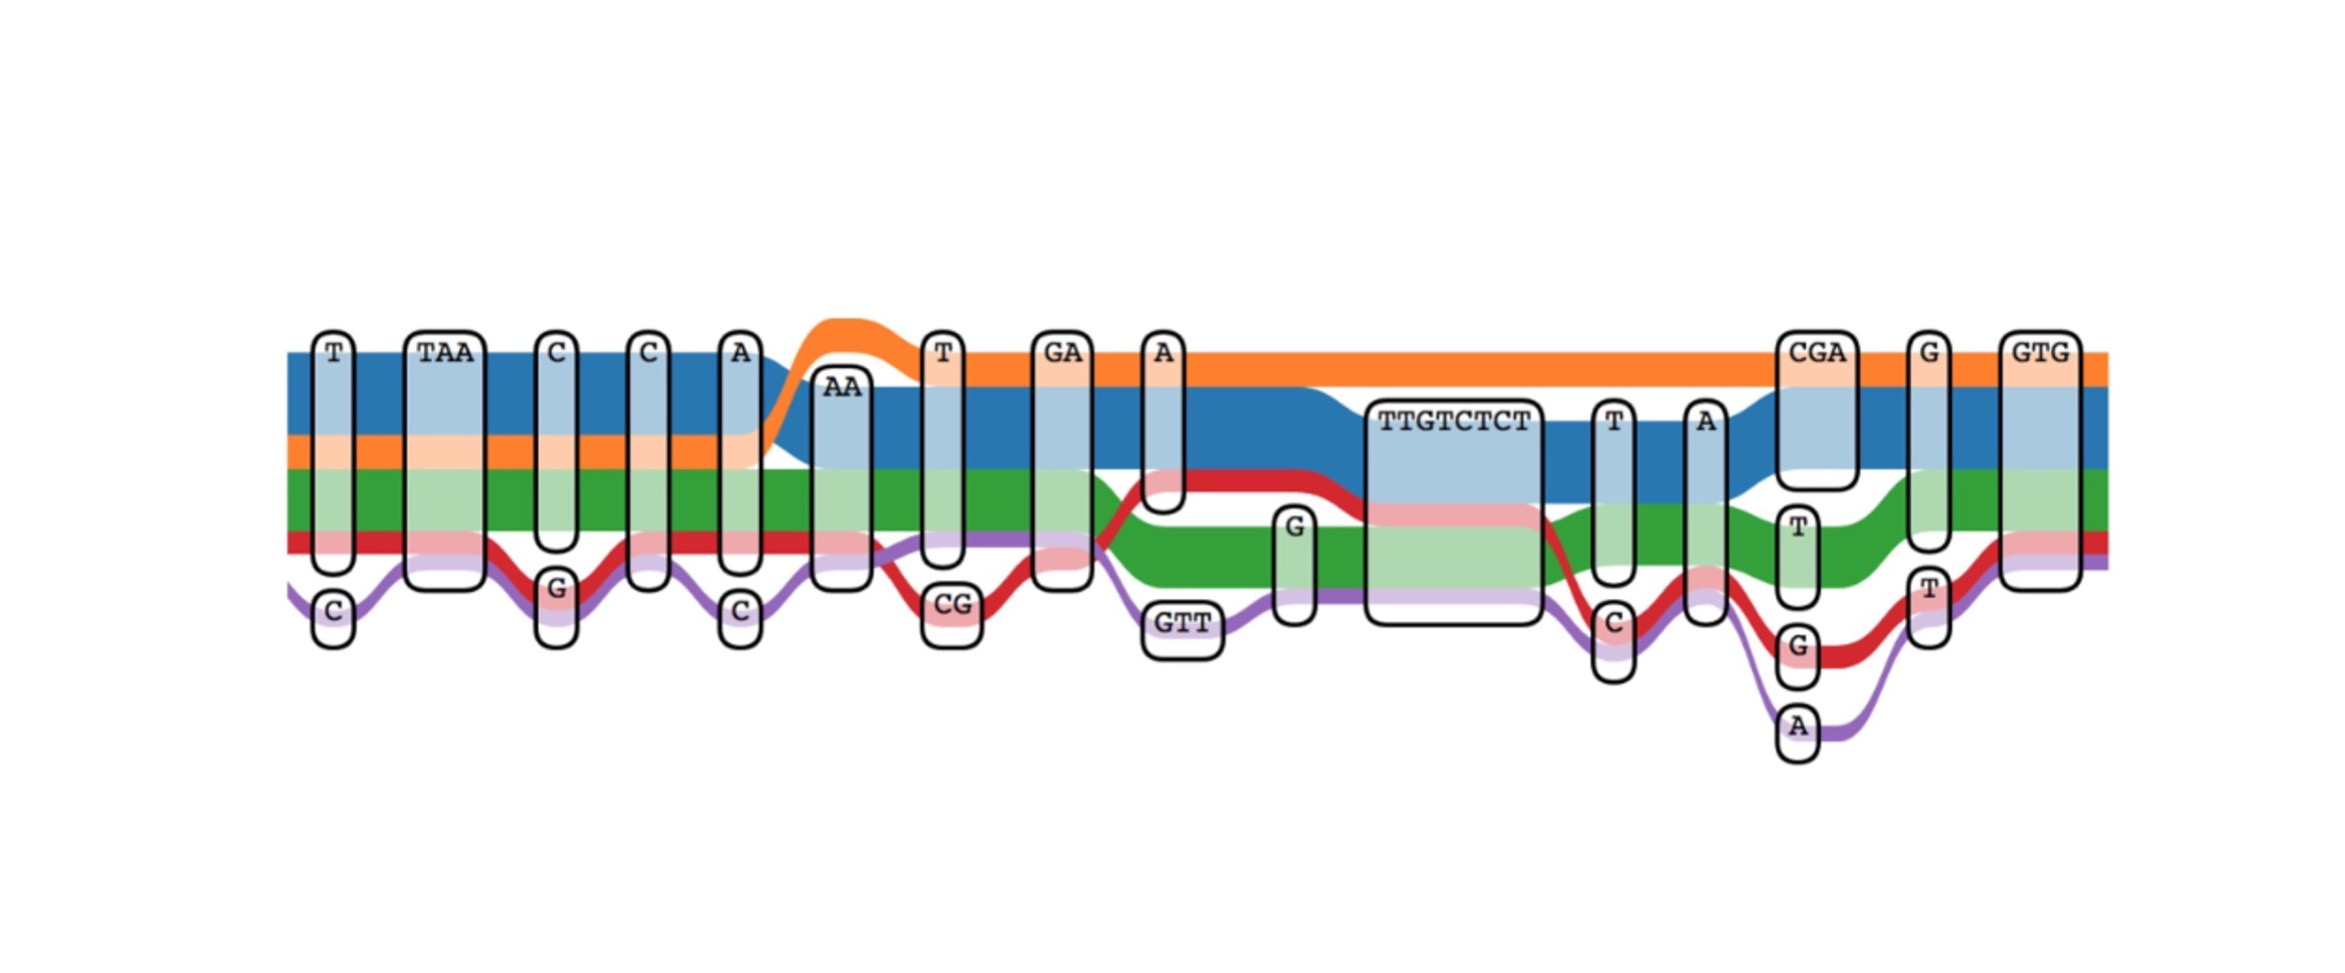
\includegraphics[width=\textwidth]{figures/vg.jpg}
% 	\caption[Genome Graphs data structure visualization]{\textbf{Genome Graphs data structure visualization.}  Each color corresponds to a path in the graph. Each path represents the genomic sequences of one of the individual genomes encoded in the Genome Graph structure.}
% 	\label{fig:vg}
% \end{figure} 


% ------ GRAFIMO
\mychapter{5}{GRAFIMO}
% In recent years, several tools have been proposed for scanning regulatory DNA regions, such as enhancers or promoters, with the goal of predicting which TF may bind these genomic locations. Importantly, it has been shown that regulatory motifs are under purifying selection \citep{li2015human,  vorontsov2016negative}, and mutations occurring in these regions can lead to deleterious consequences on the transcriptional states of a cell \citep{guo2018mutation}. In fact, mutations can weaken, disrupt or create new TFBS and therefore alter expression of nearby genes. Mutations altering TFBS can occur in haplotypes that are conserved within a population or private to even a single individual, and can correspond to different phenotypic behaviour \citep{kasowski2010variation}. For these reasons, population-level analysis of variability in TFBSs is of crucial importance to understand the effect of common or rare variants to gene regulation. Recently, a new class of methods and data structures based on genome graphs have enabled us to succinctly record and efficiently query thousands of genomes.  Genome graphs optimally encode shared and individual haplotypes based on a population of individuals. An efficient and scalable implementation of this approach called variation graphs (VGs) has been recently proposed \citep{garrison2018variation}.  VGs offer new opportunities to extend classic genome analyses originally designed for a single reference sequence to a panel of individuals. Moreover, by encoding individual haplotypes, VGs have been shown to be an effective framework to capture the potential effects of personal genetic variants on functional genomic regions profiled by ChIP-seq of histone marks \citep{groza2020personalized} 
Over the past decade, significant strides have been made in the development of methods to search known TFBS on linear reference genomes \citep{tognon2023survey, boeva2016analysis}. Notable examples include FIMO \citep{grant2011fimo} and MOODS \citep{korhonen2009moods}. They scan a set of genomic sequences searching for potential occurrences of known TFBS represented as PWMs. Other tools, such as is-rSNP, TRAP, and atSNP \citep{macintyre2010rsnp, thomas2011transcription, zuo2015atsnp}, were introduced to accommodate SNPs and short indels in the sequences to scan. However, these tools fall short in considering individual haplotypes and providing summaries of the frequency of these events in a population, limiting their applicability to precision medicine contexts. To address these challenges, we developed \grafimo (GRAph-based Finding of Infividual Motif Occurrences) \citep{tognon2021grafimo}, a novel tool performing variant- and haplotype aware identification of known TFBS in genome graphs. By leveraging genome graphs, \grafimo accounts for population-wide and individual-specific genetic variation while searching TFBSs. We demonstrate the utility of \grafimo by searching TFBS on a genome graph encoding the haplotypes from all individuals sequenced by the 1000 Genomes Project (1KGP) \citep{siva20081000, zheng2017alignment}. This innovative approach provides a more nuanced understanding of TF-DNA interaction dynamics in the context of population-wide genetic diversity. \grafimo overcomes the limitations of competitor motif scanning tools, providing a computational framework to predict the impact of genetic variation on TFs' binding landscape in precision medicine contexts.

% ----- Design and implementation
\section{Design and implementation}
\grafimo is a command-line tool enabling an efficient variant- and haplotype-aware search of known TFBS, within a population of individuals encoded in a genome graph. \grafimo provides two main functionalities: genome graph construction from user data, and the search of one or more TFBS motifs on input precomputed graphs. Briefly, given a TF motif PWM and a set of genomic regions, \grafimo leverages genome graphs to efficiently scan and report all the TFBS candidates and their frequencies in a single pass. Along with the motif candidates, \grafimo reports the predicted changes in binding affinity mediated by the genetic variants embedded in the graph. \grafimo is written in Python3 and Cython and it has been designed to interface with \emph{vg} toolkit to handle genome graphs.

% ---- Genome graph construction
\subsection{Genome variation graph construction}
\grafimo offers an intuitive command-line interface for constructing genome graphs from user data, when needed. Given a reference genome (FASTA format) and a set of genomic variants (VCF format), \grafimo seamlessly interfaces with the \emph{vg} toolkit to build the genome graphs (\texttt{VG} format) and its indexes (\texttt{XG} \citep{garrison2018variation} and \texttt{GBWT} \citep{siren2020haplotype, novak2017graph} formats). The two indexes are required to perform efficient graph traversal and track the haplotypes embedded in the data structure. To minimize the footprint of the genome graph files, \grafimo construct a graph per chromosome. Moreover, this graph construction design speeds-up the TFBS motif search by allowing to scan different chromosomes in parallel. Alternatively, for systems with limited RAM, the search can be conducted one chromosome at a time, providing flexibility in resource usage.

% ---- Transcription factor binding site motif search
%
%  ***** Comment:
% MT: should I describe the exact procedures to compute the PSSM and the statistical significance? Appendix
%
\subsection{Transcription factor binding site motif search}
The TFBS motif search in \grafimo requires a set of genomes embedded in a genome graph (\texttt{XG} format), a database of known TF motif PWMs (MEME or JASPAR formats), and a set of genomic regions (BED format). \grafimo reports all the potential TFBS motif occurrences found in the input regions and their associated statistical significance (\textbf{Fig.\ref{fig:grafimo1}}). To identify potential TFBS, \grafimo employs a sliding window approach with a window length of $k$, where $k$ is the query motif width. The window traverses the paths in the graphs that correspond to the genome sequences encoded in it (\textbf{Fig.\ref{fig:grafimo1}(B)}). This process is accomplished by an extension to the \texttt{vg find} functionality, using the graph's \texttt{GBWT} index to explore the $k$-mer space, while considering the embedded haplotypes \citep{siren2020haplotype}. By default, \grafimo focuses its search on paths corresponding to observed haplotypes, but it also provides an option to consider all possible recombinants, even if absent in any embedded sample. The significance (log-likelihood) of each TFBS candidate is determined by evaluating the nucleotide preferences encoded in the motif PWM, akin to FIMO \citep{grant2011fimo}. Specifically, the PWM undergoes processing into a Position Specific Scoring Matrix (PSSM) (\textbf{Fig.\ref{fig:grafimo1}(A)}). The resulting PSSM log-likelihood values are scaled within the range $[0, 1000]$. The scaling allows efficient statistical significance ($P$-value) computations via dynamic programming \citep{grant2011fimo}. Subsequently $P$-values undergo conversion to $q$-values through the Benjamini-Hochberg procedure to correct for multiple hypothesis testing. In this procedure, all $P$-values correspond to all the $k$-mer-paths extracted within the scanned graph's regions. Additionally, \grafimo provides insights into the number of haplotypes in which a significant motif is observed, along with its presence in the reference genome and/or alternative genomes (\textbf{Fig.\ref{fig:grafimo1}(B)}). 

% - figure: GRAFIMO TF motif search workflow
\begin{figure}
	\centering
	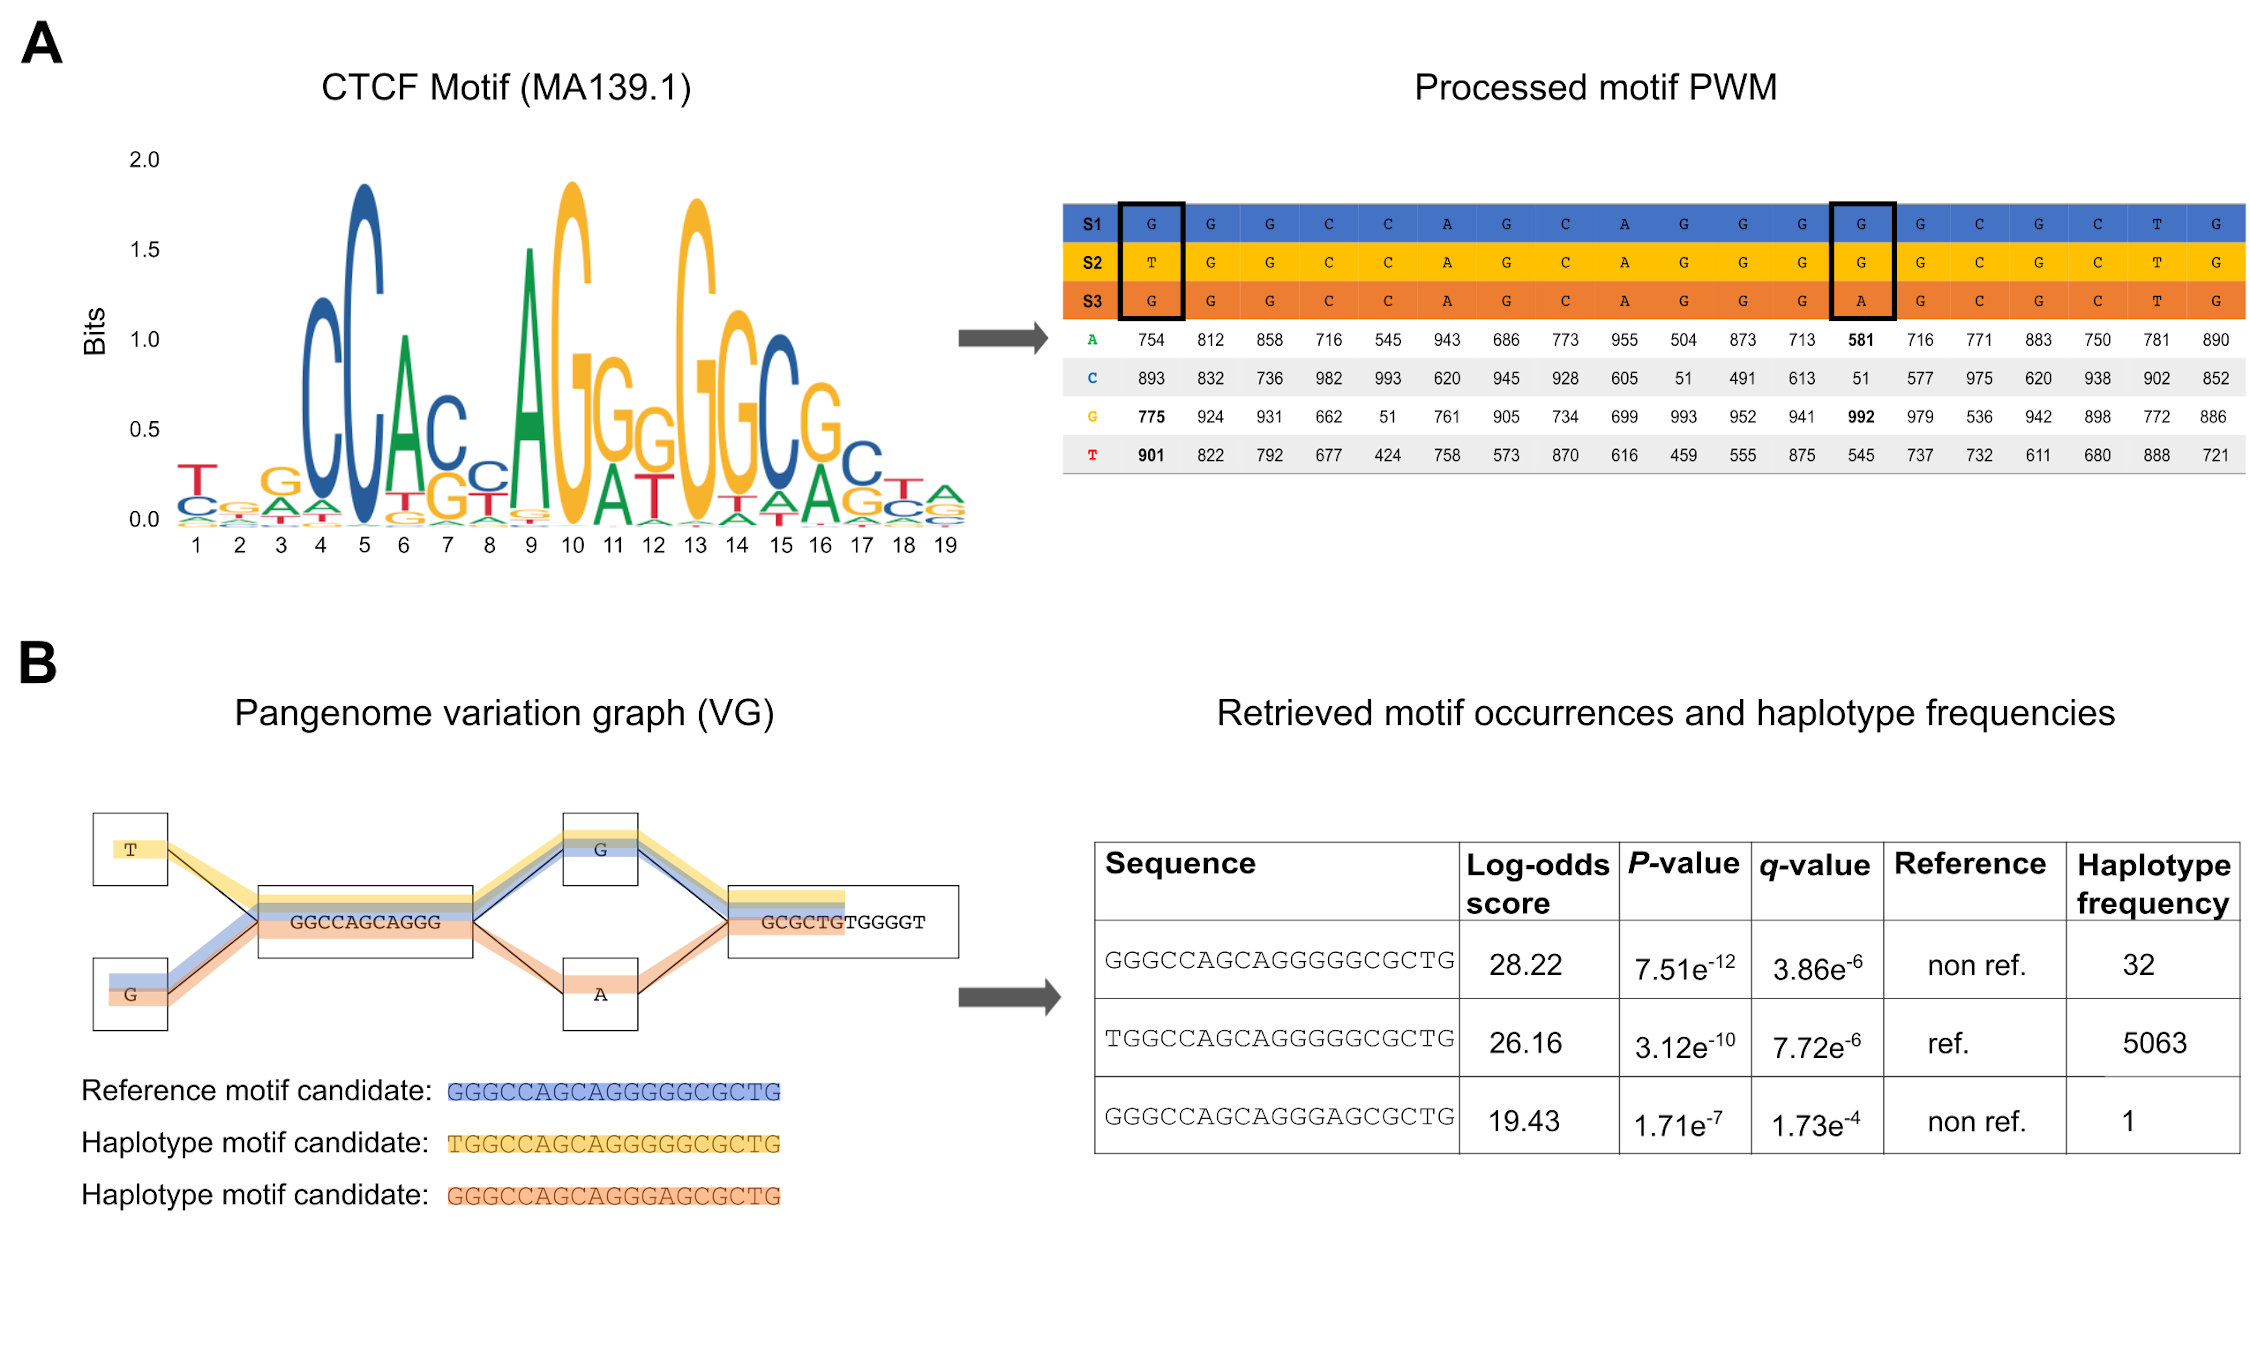
\includegraphics[width=\textwidth]{figures/grafimo1.png}
	\caption[\grafimo TF motif search workflow.]{\textbf{\grafimo TF motif search workflow. (A)} The motif PWM (in MEME or JASPAR format) is processed and its values are scaled in the range [0, 1000]. The resulting score matrix is used to assign a score and a corresponding P-value to each motif occurrence candidate. In the final report \grafimo returns the corresponding log-odds scores, which are retrieved from the scaled values. \textbf{(B)} \grafimo slides a window of length k, where k is the motif width, along the haplotypes (paths in the graph) of the genomes used to build the VG. The resulting sequences are scored using the motif scoring matrix and are statistically tested assigning them the corresponding P-value and q-value. Moreover, for each entry is assigned a flag value stating if it belongs to the reference genome sequence ("ref") or contains genomic variants ("non.ref") and is computed the number of haplotypes in which the sequence appears.}
	\label{fig:grafimo1}
\end{figure} 

% ---- Report generation
\subsection{Report generation}
\grafimo interface has been designed with inspiration drawn from FIMO, allowing seamless integration into pipelines and workflows originally built on FIMO. Similar to FIMO, \grafimo generates three distinct reports: a tab-delimited file (TSV), an HTML report, and a GFF3 file compatible with the UCSC Genome Browser \citep{lee2020ucsc}. The TSV report (\textbf{Fig.\ref{fig:grafimo-tsv}}) lists each found candidate TFBS along with its score, genomic location (start, stop, and strand), and statistical significance ($P$-value and $q$-value). Moreover, it reports the number of haplotypes in which each motif candidate has been observed, with a flag value highlighting whether the occurrence was found only on alternative haplotypes or also in the reference sequence. \grafimo also provides an HTML version of the TSV report (\textbf{Fig.\ref{fig:grafimo-html}}), that can be easily explored with any web browser. The GFF3 report is compatible with the UCSC Genome Browser, allowing users to load it as a custom track (\textbf{Fig.\ref{fig:grafimo-genome-browser}}). This enables the visualization and exploration of the identified TFBS candidates alongside additional annotations available in the Genome Browser, such as nearby genes, enhancers, promoters, or pathogenic variants sourced from the ClinVar database \citep{landrum2020clinvar}.

% - figure: GRAFIMO TSV summary report
\begin{figure}
    \centering
    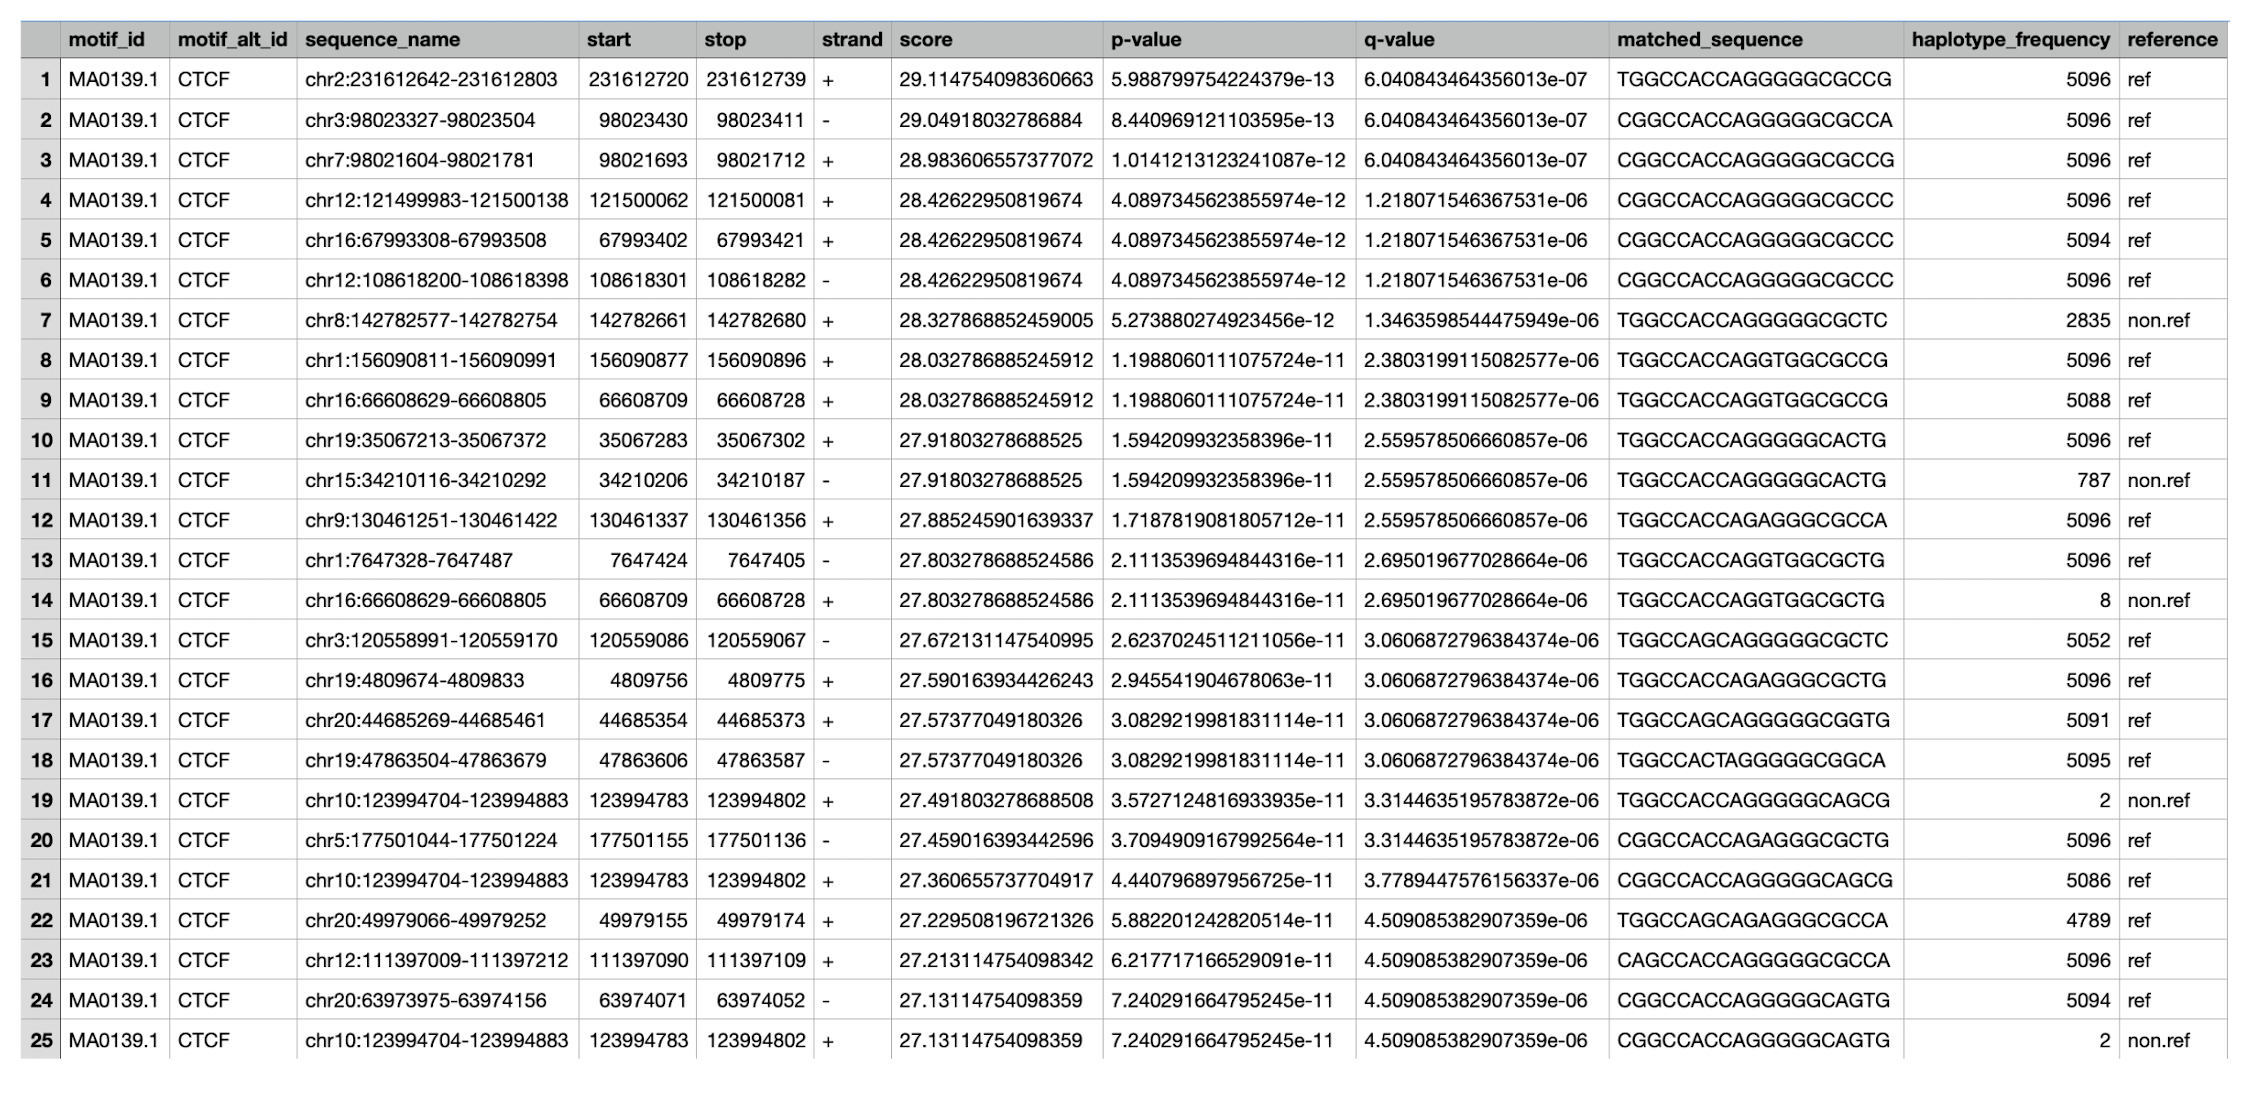
\includegraphics[width=\textwidth]{figures/grafimo-tsv-report.png}
    \caption[\grafimo TSV summary report]{\textbf{\grafimo TSV summary report.} The tab-delimited report shows the first 25 potential CTCF occurrences retrieved by \grafimo, searching CTCF motif in ChIP-seq peak regions on A549 cell line (ENCODE experiment ENCFF816XLT).}
    \label{fig:grafimo-tsv}
\end{figure}

% - figure: GRAFIMO HTML summary report
\begin{figure}
    \centering
    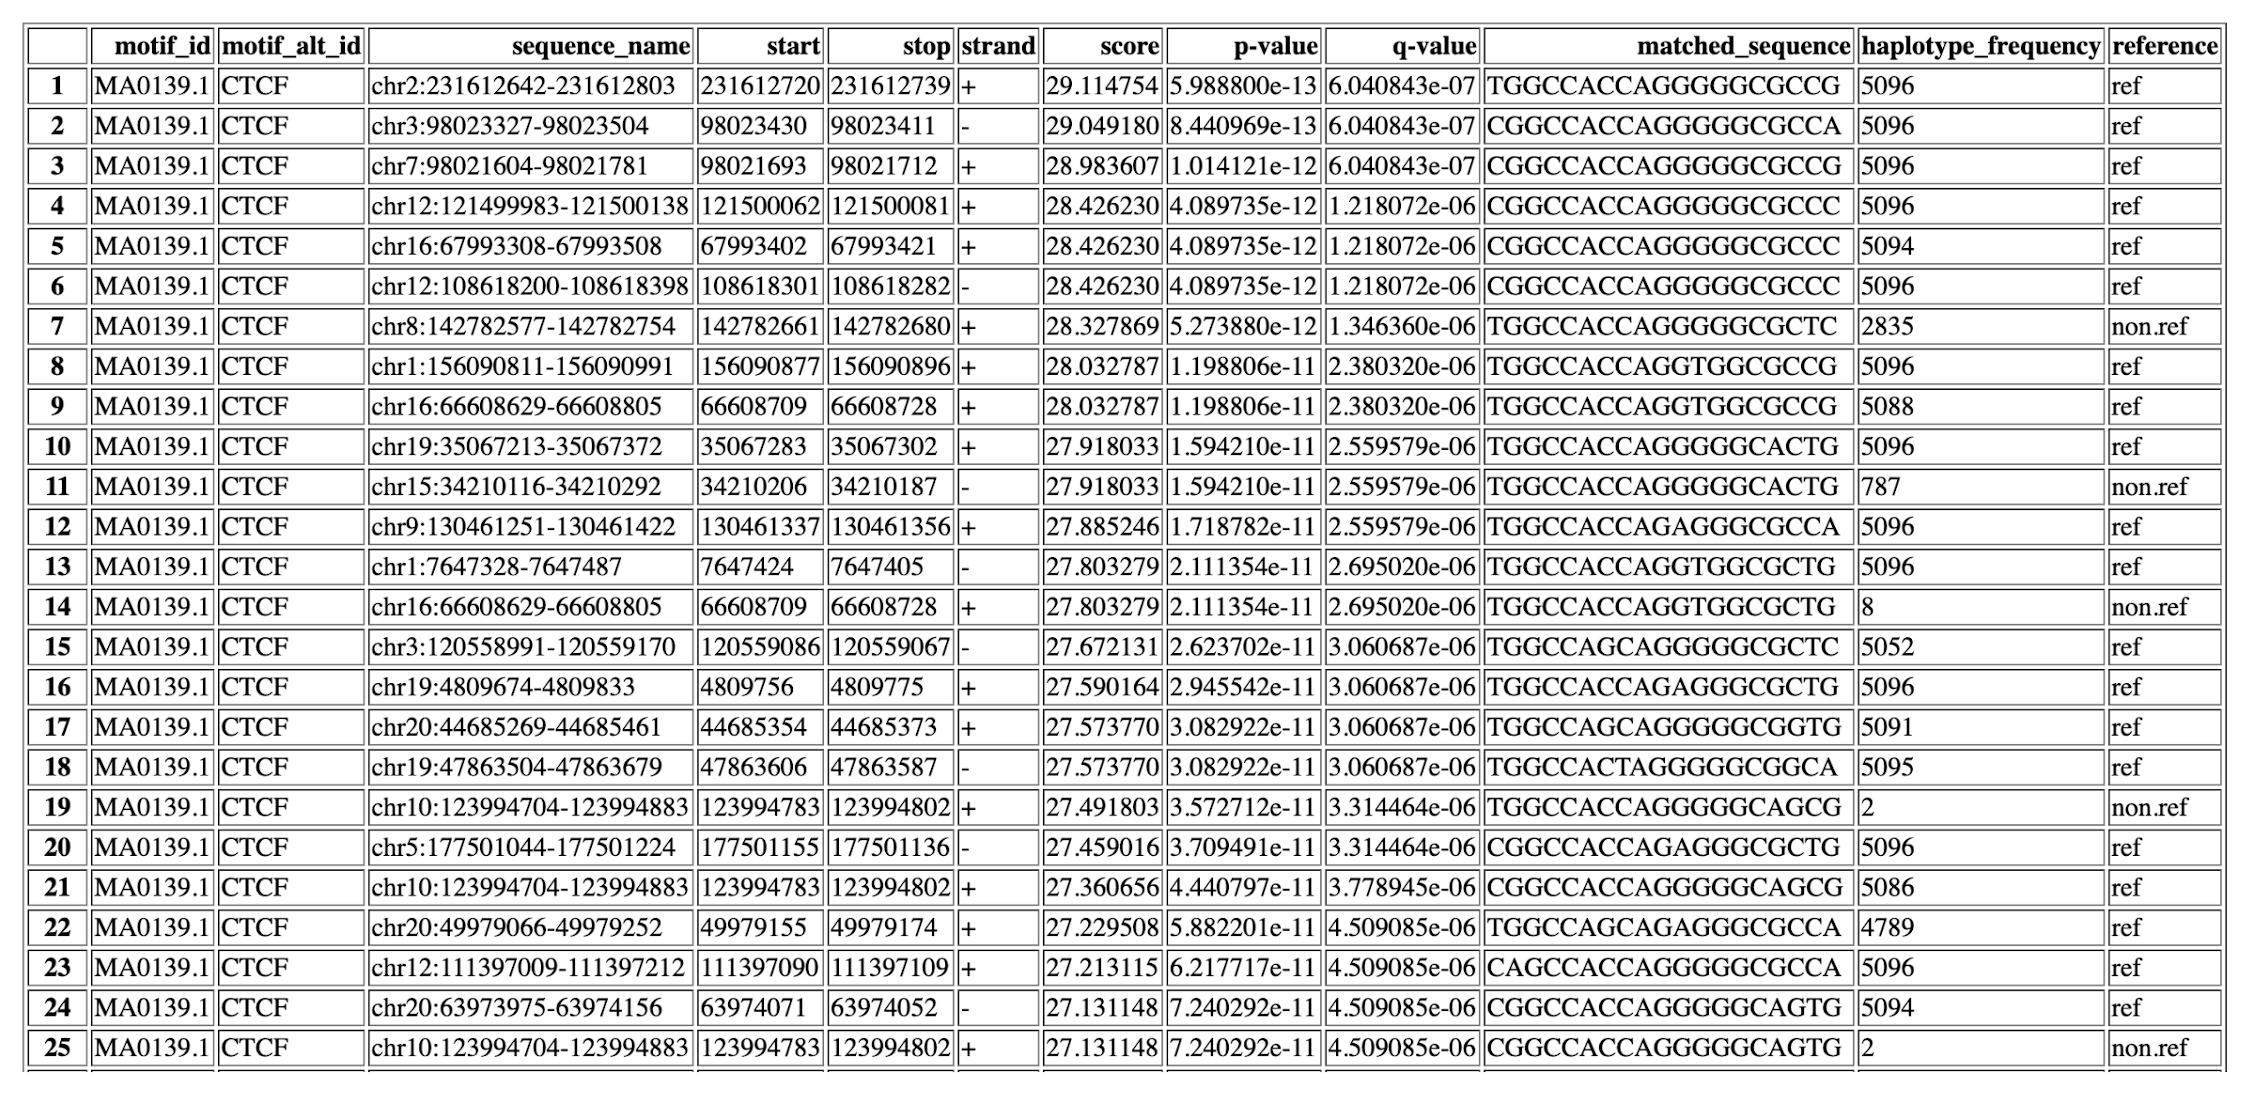
\includegraphics[width=\textwidth]{figures/grafimo-html.png}
    \caption[\grafimo HTML summary report]{\textbf{\grafimo HTML summary report.} The HTML report displays the first 25 potential CTCF occurrences retrieved by searching CTCF motif occurrences with \grafimo on ChIP-seq regions on A549 cell line (ENCODE experiment ENCFF816XLT).}
    \label{fig:grafimo-html}
\end{figure}

% - figure: GFF3 track returned by GRAFIMO and loaded on the UCSC Genome Browser 
\begin{figure}
    \centering
    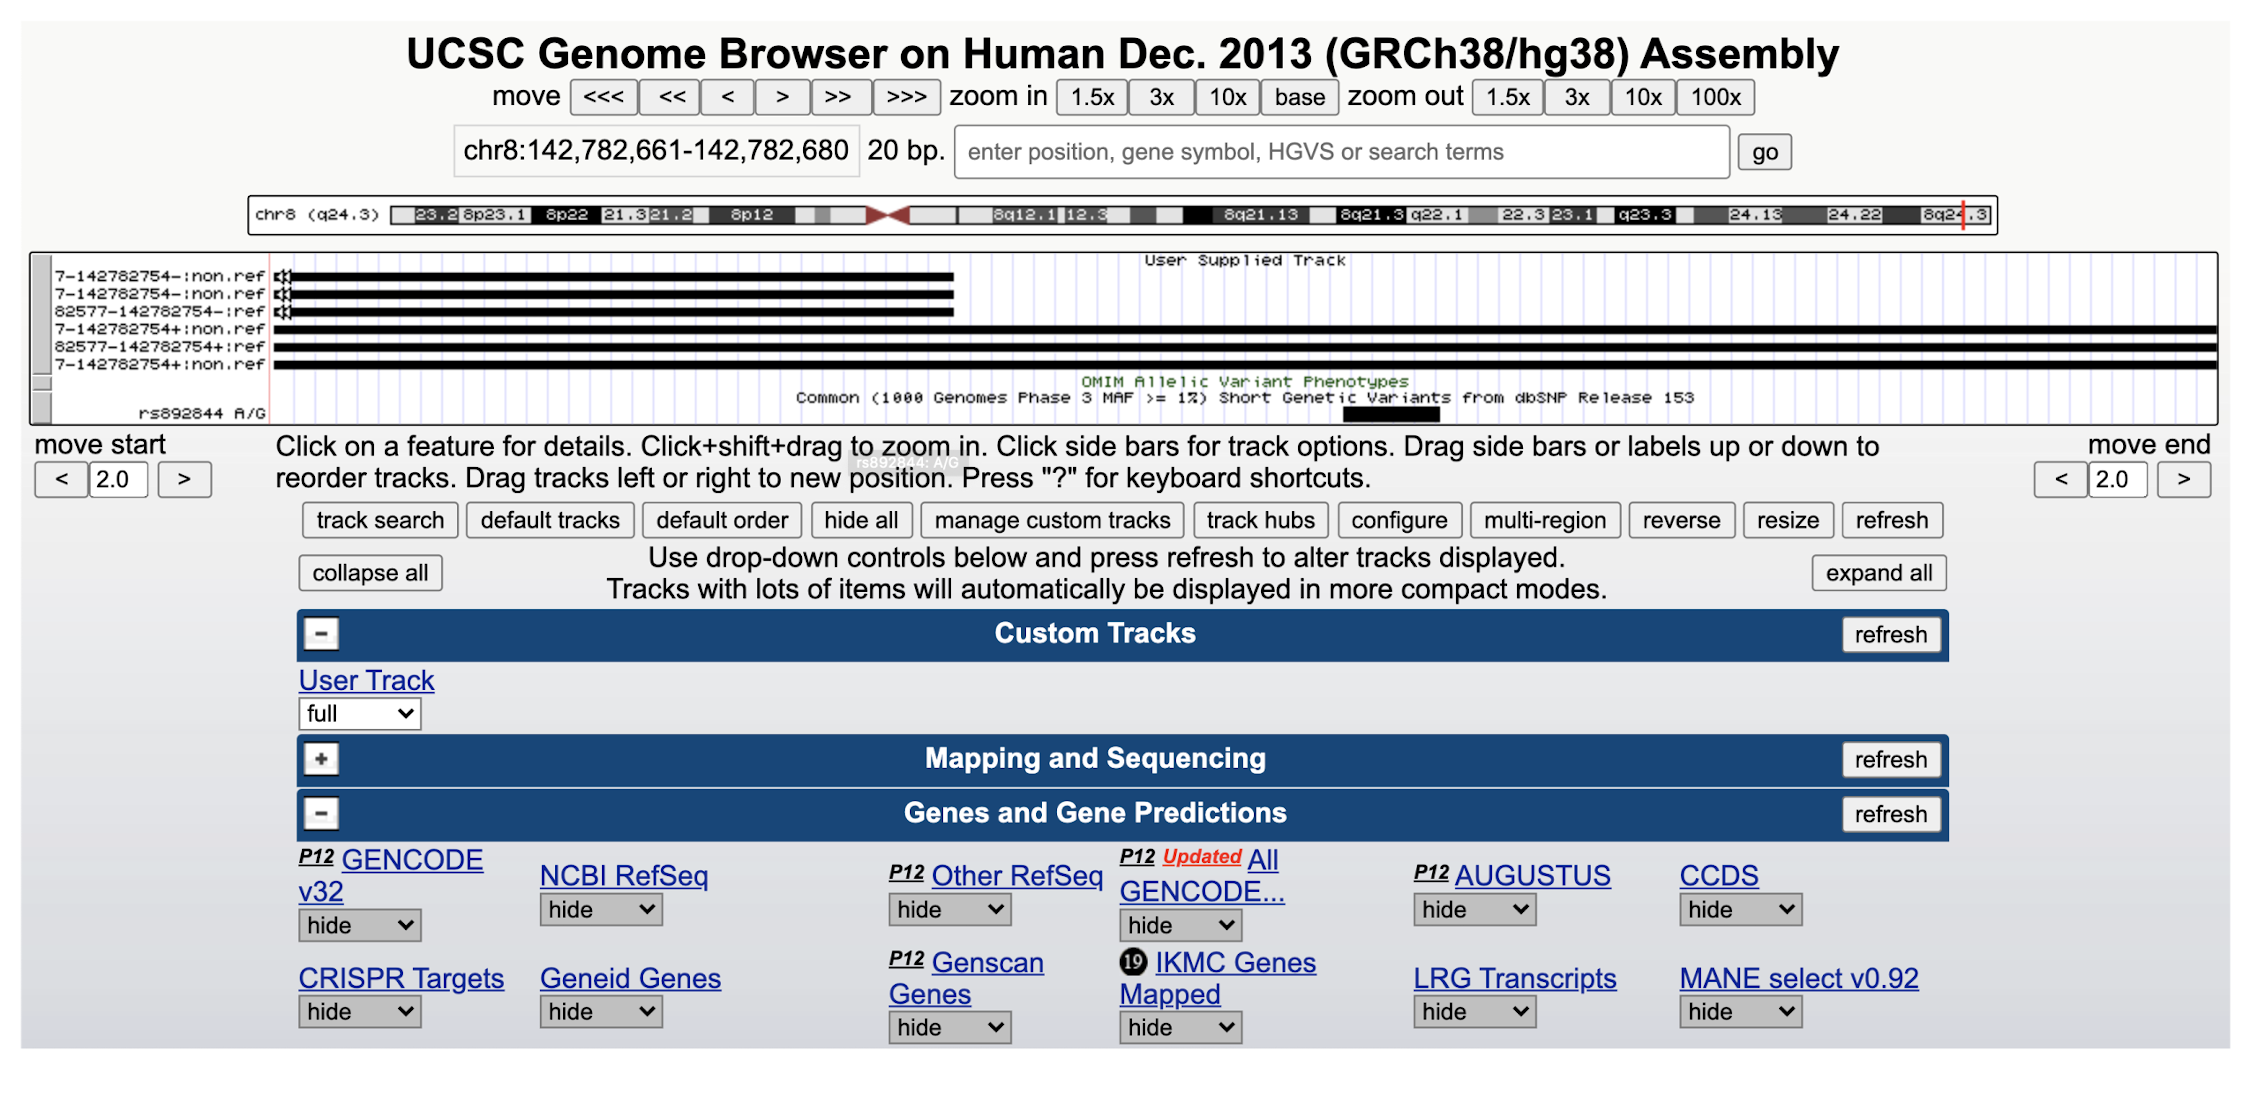
\includegraphics[width=\textwidth]{figures/grafimo-genome-browser.png}
    \caption[GFF3 track returned by \grafimo and loaded on the UCSC Genome Browser]{\textbf{GFF3 track returned by GRAFIMO and loaded on the UCSC Genome Browser.} \grafimo produces a GFF3 report which can be loaded on the UCSC Genome Browser. The custom track loaded in the example shows three potential CTCF occurrences (region chr8:142,782,661-142,782,680) recovered by \grafimo, which overlap a dbSNP annotated variant (rs892844).}
    \label{fig:grafimo-genome-browser}
\end{figure}

% ----- Searching motif occurrences with GRAFIMO
\section{Searching motif occurrences with \grafimo}
\grafimo's main aim is to investigate the potential impact of genetic variants on the binding affinity of putative TFBS across a set of individuals. By leveraging genome graphs, \grafimo may recover additional sites that might be missed when considering linear reference genomes exclusively, without accounting for genetic variants. To showcase its utility, we constructed a genome graph based on 2,548 individuals from 1KGP phase 3 (hg38 human genome assembly) \citep{zheng2017alignment, lowy2019variant}. The resulting graph encoded their genetic variants ($\sim$78 millions, SNPs and indels (\textbf{Table 
\ref{table-1KGP-variants}})) and phased haplotypes (total of 5,096 haplotypes). Subsequently, we searched the graph for putative TFBS of three TF motifs retrieved from the JASPAR database \citep{sandelin2004jaspar, fornes2020jaspar}: CTCF (JASPAR ID MA0139.1), ATF3 (JASPAR ID MA0605.2), and GATA1 (JASPAR ID MA0035.4) (\textbf{Fig.\ref{fig:grafimo-motifs}}). The three motifs exhibit diversity in length (from 11 to 19 bp), information content, and evolutionary conservation. To investigate regions with likely true binding events, we focused our analysis on ChIP-seq peak regions in six different cell lines (A549, GM12878, H1, HepG2, K562, MCF-7) retrieved from the ENCODE Project database \citep{encode2012integrated, davis2018encyclopedia} (\textbf{Table \ref{tab:table-encode-experiment}}). For each TF, we systematically acquired the optimal IDR thresholded peaks from ENCODE (bigBED format). Subsequently, we employed UCSC's \texttt{bigBedToBed} tool \citep{kent2010bigwig} to convert each bigBED file into its corresponding BED. To enhance data quality, we filtered the resulting BED files, excluding features mapped to non-canonical chromosomes. The filtered BEDs were then subjected to sorting based on both $q$-values and peak signals. This sorting allowed us to prioritize the identification of the most informative regions, specifically selecting the top 3,000 peaks for each experiment. Then, we performed a comprehensive scan on the prioritized regions using \grafimo. In our subsequent downstream analyses, we retained those sites that exhibited a $P$-value $< 1e^{-4}$. This stringent threshold ensured a focus on statistically significant potential motif occurrences. Finally, we considered the sites meeting these criteria as potential binding sites for the respective TFs under investigation. Based on the retrieved sites, we consistently observed across the three investigated TFs that genetic variants can significantly affect the estimated binding affinity. 

% - table: Genetic variants in the 1KGP genome graphs
\begin{table}[!]
    \centering
    \begin{tabular}{|p{4cm}|p{6cm}|}
        \hline
        \textbf{Chromosome} & \textbf{Number of genetic variants} \\
        \hline
        Chr1 & 6,191,833\\
        \hline
        Chr2 & 6,790,551\\
        \hline
        Chr3 & 5,641,493\\
        \hline
        Chr4 & 5,477,810\\
        \hline
        Chr5 & 5,115,036\\
        \hline
        Chr6 & 4,863,337\\
        \hline
        Chr7 & 4,511,408\\
        \hline
        Chr8 & 4,425,449\\
        \hline
        Chr9 & 3,384,360\\
        \hline
        Chr10 & 3,874,259\\
        \hline
        Chr11 & 3,881,791\\
        \hline
        Chr12 & 3,745,465\\
        \hline
        Chr13 & 2,760,845\\
        \hline
        Chr14 & 2,548,903\\
        \hline
        Chr15 & 2,301,453\\
        \hline
        Chr16 & 2,548,920\\
        \hline
        Chr17 & 2,209,149\\
        \hline
        Chr18 & 2,189,529\\
        \hline
        Chr19 & 1,738,824\\
        \hline
        Chr20 & 1,817,492\\
        \hline
        Chr21 & 1,045,269\\
        \hline
        Chr22 & 1,059,079\\
        \hline
        ChrX & 106,963\\
        \hline
    \end{tabular}
    \caption[Genetic variants in the 1KGP genome graphs]{\textbf{Genetic variants in the 1KGP genome graphs.} Number of genetic variants (SNPs and indels) in the genome graph constructed using 1KGP phase 3 on hg38 data. The variants belong to 2,548 individuals from 26 populations. In total the genome graphs encoded $\sim$78 millions variants.}
    \label{table-1KGP-variants}
\end{table}

% - table: ENCODE ChIP-seq experiment codes
\begin{table}[!]
    \centering
    \resizebox{\columnwidth}{!}{%
    \begin{tabular}{|l|l|l|l|l|l|l|}
        \hline
        \textbf{Motif} & \textbf{A549} & \textbf{GM12878} & \textbf{H1} & \textbf{HepG2} & \textbf{K562} & \textbf{MCF-7} \\ \hline
        CTCF  & ENCFF816XLT & ENCFF267NYF &             & ENCFF015OJG & ENCFF895HAG                                                       & ENCFF088JWU \\ \hline
        ATF3  &             &             & ENCFF207AVV & ENCFF753WNT & ENCFF787GVU                                                       &             \\ \hline
        GATA1 &             &             &             &             & \begin{tabular}[c]{@{}l@{}}ENCFF811YFQ\\ ENCFF939ODZ\end{tabular} &             \\ \hline
    \end{tabular}%
    }
    \caption[ENCODE ChIP-seq experiments]{\textbf{ENCODE ChIP-seq experiments.} To test our software we searched potential occurrences of three transcription factor motifs (CTCF, ATF3, and GATA1) in a hg38 genome graph enriched with genetic variants and haplotypes of 2,548 individuals from 1000 Genomes Project phase 3.}
    \label{tab:table-encode-experiment}
\end{table}

% - figure: Transcription factor motifs used to test GRAFIMO
\begin{figure}[!]
    \centering
    \includegraphics[width=\textwidth]{figures/grafimo-motifs.png}
    \caption[Transcription factor motifs used to test \grafimo]{\textbf{Transcription factor motifs used to test \grafimo.} Transcription factor binding site motifs of \textbf{(A)} CTCF, \textbf{(B)} ATF3, and \textbf{(C)} GATA1.}
    \label{fig:grafimo-motifs}
\end{figure}

% ---- Searching for CTCF occurrences
\subsection{Searching for CTCF occurrences}
CTCF is a zinc-finger transcription factor involved in transcriptional regulation, playing a pivotal role in epigenetic control \citep{ishihara2006ctcf}, and functioning as a tumor suppressor \citep{fiorentino2012tumor}. In our experiments, we performed a targeted search for CTCF motif (JASPAR ID MA0139.1) (\textbf{Fig.\ref{fig:grafimo-motifs} (A)}) occurrences within the 1KGP genome graph. Interestingly, we found a substantial number of CTCF motif occurrences exclusive to non-reference haplotypes, indicating that a significant pool of potential TFBS is overlooked when scanning the genome without considering genetic variants (\textbf{Fig.\ref{fig:grafimo-ctcf} (A)}). Furthermore, our analysis identified several highly significant CTCF occurrences within rare haplotypes (\textbf{Fig.\ref{fig:grafimo-ctcf} (B)}), that may influence gene expression in individuals showing these haplotypes. We investigated the genomic locations of significant motif occurrences to assess how individual binding sites might be affected by genetic diversity--whether disrupted, created, or modulated. Interestingly, our experiments revealed that 6.13\% of potential CTCF binding sites were exclusive to non-reference haplotypes, 5.94\% were disrupted by variants in non-reference haplotypes, and approximately 30\% retained significance in non-reference haplotypes, but with different binding scores (\textbf{Fig.\ref{fig:grafimo-ctcf} (C)}). Notably, a considerable portion of putative binding sites recovered solely on individual haplotypes exhibited population specificity. For instance, 24.66\%, 6.74\%, 5.68\%, 13.01\%, and 12.52\% of potential CTCF binding sites retrieved exclusively from individual haplotypes were specific to AFR, EUR, AMR, SAS, and EAS populations, respectively (\textbf{Fig.\ref{fig:grafimo-ctcf} (D)}). Among the unique motif occurrences identified exclusively in non-reference haplotypes in CTCF ChIP-seq peaks, we uncovered a TFBS (chr19:506,910-506,929) that illustrates the pitfalls of relying solely on reference genomes for motif scanning. In this genomic locus, we identified a heterozygous SNP aligning with position 10 of the CTCF matrix, that significantly modulates the binding affinity of the corresponding binding site. By inspecting ChIP-seq reads (experiment ENCSR000DZN on GM12878), an allelic imbalance emerged towards the alternative allele. The alternative allele G exhibited a clear prevalence (70.59\% of reads), while the reference allele A lagged behind at 29.41\% of reads. This allelic imbalance is not observed in the control reads (experiment ENCSR000EYX) (\textbf{Fig.\ref{fig:grafimo-allelic-imbalance}}).

% - figure: Searching CTCF motif on genome graphs using GRAFIMO provides insights on the impact of genetic diversity on putative binding sites
\begin{figure}
    \centering
    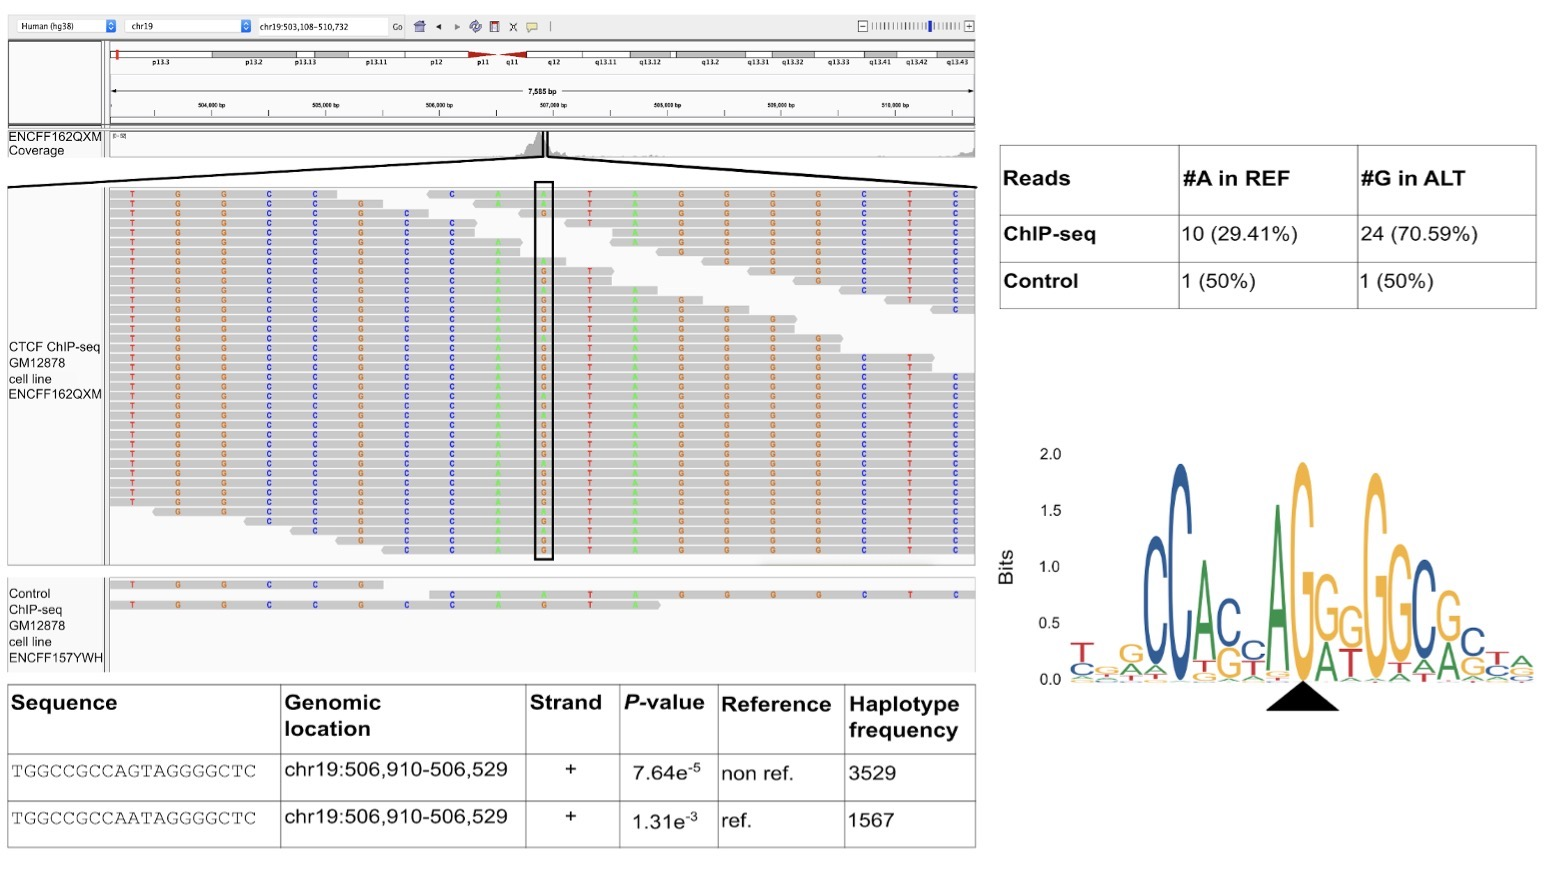
\includegraphics[width=\textwidth]{figures/grafimo2.jpg}
    \caption[Searching CTCF motif on genome graphs using \grafimo provides insights on the impact of genetic diversity on putative binding sites]{\textbf{Searching CTCF motif on genome graphs using \grafimo provides insights on the impact of genetic diversity on putative binding sites. (A)} Statistically significant ($P$-value $< 1e^{-4}$) and non-significant potential CTCF occurrences found in the reference and haplotype sequences found using \grafimo on 1KGP genome graph. \textbf{(B)} Statistical significance of the identified CTCF occurrences and their frequency within the haplotypes embedded in the genome graph. \textbf{(C)} Percentage of statistically significant potential CTCF binding sites found only in the reference genome, only in alternative haplotypes, and with their binding scores modulated by 1KGP genetic variants. \textbf{(D)} Percentage of population-specific and common (shared by two or more populations) CTCF binding sites found in individual haplotypes.}
    \label{fig:grafimo-ctcf}
\end{figure}

% - figure: Considering genomic diversity, GRAFIMO captures additional binding events
\begin{figure}
    \centering
    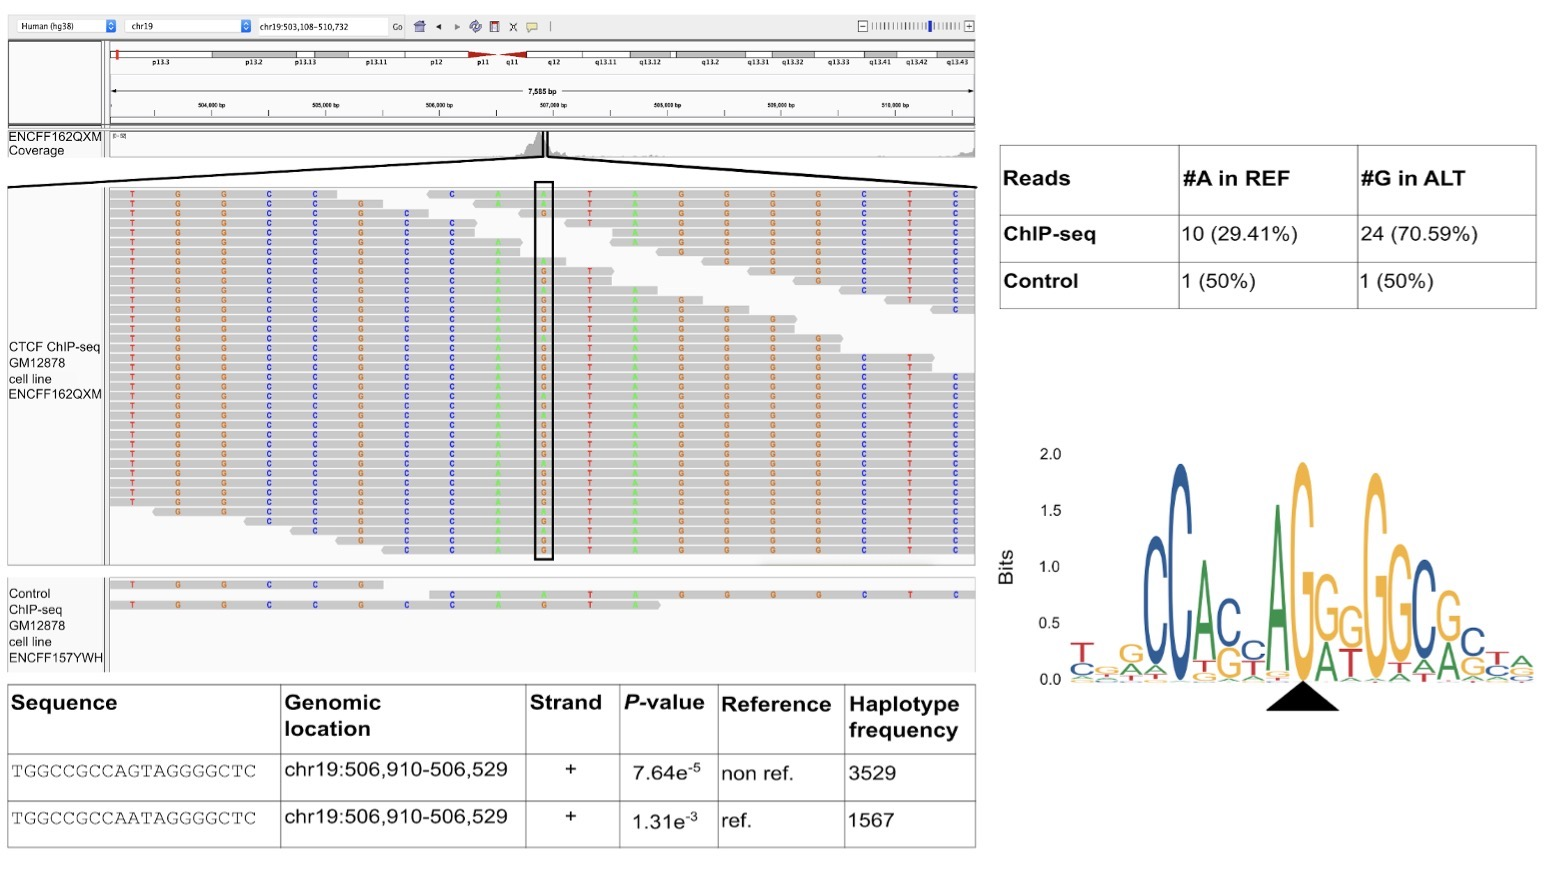
\includegraphics[width=\textwidth]{figures/grafimo3.jpg}
    \caption[Considering genomic diversity, \grafimo captures additional binding events]{\textbf{Considering genomic diversity, \grafimo captures additional binding events.} \grafimo reports a potential CTCF binding site at chr19:506,910-506,929 exclusively present in haplotype sequences. The binding site was identified by scanning CTCF ChIP-seq peaks (experiment ENCSR000DZN on GM12878). The analysis of ChIP-seq reads (ENCFF162QXM) unveils an allelic imbalance at position 10 of the motif, towards the alternative allele (G). \grafimo accurately captures this imbalance by reporting sequences carrying a G at position 10 (as found in the alternative haplotypes), while the potential TFBS on the reference, which carries an A, is not reported as statistically significant. This discrepancy aligns with CTCF motif logo, which illustrates G as the dominant nucleotide at position 10.}
    \label{fig:grafimo-allelic-imbalance}
\end{figure}

% ---- Searching for ATF3 occurrences
\subsection{Searching for ATF3 occurrences}
Activating Transcription Factor 3 (ATF3) is a member of the cAMP responsive element-binding family, exhibits increased activity in response to physiological stress across diverse tissues \citep{chen1996analysis}. Moreover, ATF3 has versatile roles in immunity and cancer \citep{thompson2009atf3}. ATF3 binds to short conserved DNA sequences. In our investigations, we searched ATF3 motif (JASPAR ID MA0605.2) (\textbf{Fig.\ref{fig:grafimo-motifs} (B)}) occurrences within the 1KGP genome graph. For subsequent analyses we considered ATF3 occurrences with $P$-value $< 1e^{-4}$ as potential binding sites. Our results unveiled several potential motif occurrences that would be lost scanning only the reference genome sequences (\textbf{Fig.\ref{fig:grafimo-atf3} (A)}). Additionally, we observed that several ATF3 motif occurrences with high statistical significance were identified in alternative haplotypes (\textbf{Fig.\ref{fig:grafimo-atf3} (B)}). Furthermore, we observed that 7.03\% of potential ATF3 binding sites are exclusively identified in non-reference haplotype sequences, 11.28\% are disrupted by genomic variants, and approximately 13\% of ATF3 TFBS maintain significance in non-reference haplotypes but exhibit different binding scores (\textbf{Fig.\ref{fig:grafimo-atf3} (C)}). Importantly, a substantial fraction of putative ATF3 binding sites displayed population specificity: 19.81\%, 3.77\%, 7.55\%, 19.81\%, and 19.81\% of potential binding sites retrieved in individual haplotypes were specific to AFR, EUR, AMR, SAS, EAS populations, respectively (\textbf{Fig.\ref{fig:grafimo-atf3} (D)}). 

% - figure: Searching ATF3 motif on genome graphs using GRAFIMO provides insights on the impact of genetic diversity on putative binding sites
\begin{figure}
    \centering
    \includegraphics[width=\textwidth]{figures/grafimo-atf3.png}
    \caption[Searching ATF3 motif on genome graphs using \grafimo provides insights on the impact of genetic diversity on putative binding sites]{\textbf{Searching ATF3 motif on genome graphs using \grafimo provides insights on the impact of genetic diversity on putative binding sites. (A)} Statistically significant ($P$-value $< 1e^{-4}$) and non-significant potential ATF3 occurrences found in the reference and haplotype sequences found using \grafimo on 1KGP genome graph. \textbf{(B)} Statistical significance of the identified ATF3 occurrences and their frequency within the haplotypes embedded in the genome graph. \textbf{(C)} Percentage of statistically significant potential ATF3 binding sites found only in the reference genome, only in alternative haplotypes, and with their binding scores modulated by 1KGP genetic variants. \textbf{(D)} Percentage of population-specific and common (shared by two or more populations) ATF3 binding sites found in individual haplotypes.}
    \label{fig:grafimo-atf3}
\end{figure}

% ---- Searching for GATA1 occurrences
\subsection{Searching for GATA1 occurrences}
GATA1 is a zinc-finger transcription factor playing a pivotal role in the development of hematopoietic cell lineages \citep{calligaris1995alternative}. GATA1 binds short (11 bp) highly conserved DNA sequences. In our experiments, we searched GATA1 motif (JASPAR ID MA0035.4) (\textbf{Fig.\ref{fig:grafimo-motifs}}) occurrences within the 1KGP genome graph. In our downstream analyses we considered GATA1 occurrences with $P$-value $< 1e^{-4}$ as potential binding sites. In our experiments we observed that several GATA1 occurrences are lost when not considering genetic diversity while scanning genomic sequences (\textbf{Fig.\ref{fig:grafimo-gata1} (A)}). Moreover, several potential motif occurrences with high statistical significance were found scanning non-reference haplotypes (\textbf{Fig.\ref{fig:grafimo-gata1} (B)}). Further investigations unveiled that 9.78\% of potential GATA1 binding sites are exclusive to non-reference haplotype sequences, 12.58\% are disrupted by genetic variants, and $\sim$4\% maintain significance in non-reference haplotypes but exhibit different binding scores (\textbf{Fig.\ref{fig:grafimo-gata1} (C)}). We also identified population specific GATA1 binding sites among those retrieved only in individual haplotypes, with 25.97\% specific to AFR, 3.90\% to EUR, 9.09\% to AMR, 19.48\% to SAS, and 11.69\% to EAS populations (\textbf{Fig.\ref{fig:grafimo-gata1}(D)}).

% - figure: Searching GATA1 motif on genome graphs using GRAFIMO provides insights on the impact of genetic diversity on putative binding sites
\begin{figure}
    \centering
    \includegraphics[width=\textwidth]{figures/grafimo-gata1.png}
    \caption[Searching GATA1 motif on genome graphs using \grafimo provides insights on the impact of genetic diversity on putative binding sites]{\textbf{Searching GATA1 motif on genome graphs using \grafimo provides insights on the impact of genetic diversity on putative binding sites. (A)} Statistically significant ($P$-value $< 1e^{-4}$) and non-significant potential GATA1 occurrences found in the reference and haplotype sequences found using \grafimo on 1KGP genome graph. \textbf{(B)} Statistical significance of the identified GATA1 occurrences and their frequency within the haplotypes embedded in the genome graph. \textbf{(C)} Percentage of statistically significant potential GATA1 binding sites found only in the reference genome, only in alternative haplotypes, and with their binding scores modulated by 1KGP genetic variants. \textbf{(D)} Percentage of population-specific and common (shared by two or more populations) GATA1 binding sites found in individual haplotypes.}
    \label{fig:grafimo-gata1}
\end{figure}

% ----- Comparing GRAFIMO and FIMO
\section{Comparing \grafimo and FIMO}
To validate \grafimo accuracy, we conducted a comparative analysis with FIMO, running the latter on the same ChIP-seq regions used to test the former. FIMO and \grafimo runs were performed on a Linux-based machine with an Intel(R) Core (TM) i7-5960X 3.00GHz CPU (16 cores) and 64 GB of memory (RAM). Since FIMO scans sets of sequences given as FASTA files, for each investigated TF, we recovered the reference genome sequences representing the ChIP-seq optimal IDR thresholded peaks using BEDTools \citep{quinlan2010bedtools}. For each studied TF, we observed that \grafimo reports all potential motif occurrences identified by FIMO. Therefore, \grafimo successfully identifies additional motif candidates found in individual haplotypes embedded in the genome graph without sacrificing potential motif occurrences in the reference genome sequence. We further benchmarked \grafimo against FIMO in terms of running time and memory usage. Using CTCF motif (19 bp) as an example, we searched for potential motif occurrences on forward and reverse strands in 1000 genomic regions of human chr22 with increasing length (1 to 9 Mb). To run FIMO, for each set of genomic regions we created the corresponding FASTA file. To assess \grafimo performance we scanned chr22 genome graph without encoded variants, on the previously computed set of regions. Since FIMO does not provide a parallel implementation we run \grafimo using a single thread. Although FIMO exhibits superior speed and lower memory requirements in a single-thread scenario (\textbf{Fig.\ref{fig:grafimo-fimo-cmp1} (A)} and \textbf{(B)}), \grafimo surpasses FIMO in speed when scanning regions accounting for genetic variants of 2,548 individuals (\textbf{Fig.\ref{fig:grafimo-fimo-cmp1} (C)}). We excluded from the measurements for FIMO the overhead introduced to compute the FASTA files from the original BED files. These results were expected since FIMO is a highly optimized tool scanning linear reference genomic sequences, while \grafimo efficiency shines while scanning panels of individuals accounting for their genetic diversity. We further evaluated \grafimo performance using 1, 4, 8, and 16 threads to scan the chr22 genome graph embedding the 2,548 individuals and their genetic variants from 1KGP (\textbf{Fig.\ref{fig:grafimo-fimo-cmp2}}). As expected, using multiple threads significantly reduces running time, although memory usage remains consistent with the number of threads. For the analyses presented in the previous section each scan on average took $\sim$15 minutes and consumed around 24 GB of memory. 

% - figure: Comparing GRAFIMO and FIMO performance
\begin{figure}
    \centering
    \includegraphics[width=\textwidth]{figures/grafimo-runningtime.png}
    \caption[Comparing \grafimo and FIMO performance]{\textbf{Comparing \grafimo and FIMO performance. (A)} FIMO is faster than \grafimo (using 1 thread) when searching CTCF motif (JASPAR ID MA0139.1) on human chr22 regions (total width ranging from 1 to 9 Mb) and without accounting for genetic variants. \textbf{(B)} FIMO uses less memory than \grafimo, however it only scan reference sequences. \textbf{(C)} \grafimo is generally faster than FIMO while searching CTCF occurrences when considering genetic diversity in large panels of individuals (e.g. 1KGP phase 3), even with single thread.}
    \label{fig:grafimo-fimo-cmp1}
\end{figure}

% - figure: GRAFIMO running time efficiently scales with the number of threads
\begin{figure}
    \centering
    \includegraphics[width=\textwidth]{figures/grafimo-runningtime2.png}
    \caption[\grafimo running time efficiently scales with the number of threads]{\textbf{\grafimo running time efficiently scales with the number of threads.} By running \grafimo with multiple threads \textbf{(A)} the running time significantly decreases, while \textbf{(B)} memory usage remains similar.}
    \label{fig:grafimo-fimo-cmp2}
\end{figure}

% -- Discussion and limitations
%
% MT: TODO: discuss some GRAFIMO limitations
% 
\section{Discussion and limitations}
By leveraging genome graphs, \grafimo introduces an effective approach for investigating the impact of genetic variation on the binding landscape of transcription factors (TFs) across diverse populations. Notably, our findings revealed the presence of numerous potential and exclusive TF binding sites (TFBS) in individual haplotype sequences. Additionally, genomic variants exert a substantial influence on the binding affinity of several motif occurrence candidates identified in the reference genome sequence. This tool offers a valuable resource for prioritizing regions that could underlie individual-specific alterations in gene expression, a facet often overlooked when relying solely on reference genomes.


% ---- MotifRaptor2
\mychapter{6}{\motifraptor2}
Several studies have reported that genetic variants can enhance or disrupt TF-DNA binding affinity \citep{de2006regulatory, weinhold2014genome, wienert2015editing}. Genome-wide association studies (GWASs) have uncovered thousands of genetic variants (SNPs) associated with complex traits or human disease \citep{buniello2019nhgri}. Despite these efforts, functional studies to prioritize potential causal variants have lagged behind \citep{gallagher2018post}, resulting in a limited interpretation of the underlying pathophysiology mechanisms connecting variant to phenotype. A few missense SNPs can alter the function of a given TF by affecting its coding sequence, protein structure and therefore DNA binding capability, especially for Mendelian disease \citep{barrera2016survey}. For common diseases and complex traits, the great majority ($>$90\%) of associated SNPs are in non-coding regions and mainly in DNase I hypersensitive sites. These SNPs correspond to functionally relevant non-coding regions such as enhancers and promoters \citep{maurano2012systematic}. This observation suggests that chromatin state alterations and gene deregulation may be mediated by SNPs that modulate TF binding activities. In other words, genetic variants in these non-coding regions may perturb TF recognition sequences to enhance or disrupt TF-DNA binding events ultimately changing the downstream gene expression programs \citep{deplancke2016genetics}. Even if single non-coding SNPs may only moderately alter binding sites and are underpowered to explain gene expression programs, statistics on a set of SNPs modulating common TF binding sites could be significant enough to reveal the convergent regulatory mechanism in complex traits. The method we present is based on this key idea.Despite the fact that several approaches have been proposed to explore how TF binding sites could be affected by genetic variants, challenges remain. The next paragraphs provide a short summary and the rationale behind the development of Motif-Raptor. First, current availability of ChIP-seq data unfortunately limit the utility of tools such as MMARGE \citep{link2018mmarge}, GERV \citep{zeng2016gerv}, DeepSEA \citep{zhou2015predicting}, Basset \citep{kelley2016basset}, IMPACT \citep{amariuta2019impact}, RegulomeDB \citep{boyle2012annotation}, HaploReg4 \citep{ward2012haploreg}. In fact, these tools are extremely powerful and practical only when genome-wide maps of TF occupancy and/or chromatin marks in relevant cellular contexts are available. Therefore, in \citep{yao2021motif}, the authors found a unique value proposition in developing a framework to accommodate scenarios in which only PWM models and gene expression data are available. Second, available models based on ChIP-seq or PWM data do not systematically provide a global ranking and the significance of the TFs based on all trait-associated variants, rather a per SNP scoring. In fact, current methods based on PWM and/or DNase I-seq data, such as Combined Annotation Dependent Depletion (CADD, \citep{maurano2015large}), CENTIPEDE \citep{moyerbrailean2016genetics, pique2011accurate}, Affinity Testing for regulatory SNPs (atSNP, \citep{zuo2015atsnp}). do not provide a procedure to formally test the global effect of a set of GWAS variants on the set of overlapping TF binding sites. To solve this limitation, \motifraptor proposed a novel genome-wide statistic to prioritize putative causal TFs based on the entire set of binding sites and overlapping variants rather than single loci. Third, these methods do not consider linkage disequilibrium (LD) for the tagged loci by the GWAS-associated variants. This is important given that several non-causal SNPs have similar association scores as the true causal ones and that this potentially confound the analysis. In fact, these false positives can dilute our power of detecting the true mechanisms behind the causal variants. \motifraptor's approach tries to account for this problem based on the two following strategies. By relying on cell type-specific chromatin accessibility regions, it is already reducing the space of variants in each LD block. To implicitly account for local LD structure, \motifraptor samples the background set of chromatin accessibility regions in close proximity of the regions that are specific for each cell type. With these strategies, \motifraptor mitigates the problem by specifically looking for variants within regions that are cell type specific. Among available tools only SLDP (Signed LD Profile) \citep{reshef2018detecting} overcomes this problem and offers a genome-wide significance score for each TF, based on the directional modulation of TF binding sites by SNPs. Another tool, GREGOR (Genomic Regulatory Elements and Gwas Overlap algoRithm) \citep{schmidt2015gregor}, also explicitly accounts for LD structure to assess the enrichment on sentinel SNPs in arbitrary genomic regions (e.g. to prioritize cell types based on cell type specific annotations). \motifraptor addresses the above limitations of current approaches, by providing a cell type-specific TF-centric analysis with associated statistics, comprehensive reporting and visualization functionalities. This tool can facilitate the discovery and interpretation of the action of non-coding variants on key regulators of complex traits.
% -- Design and implementation
\subsection{Design and implementation}
\motifraptor pipeline consists of three main steps (\textbf{Fig.\ref{fig:motifraptor1}}). (i) TCharacterize important cell-types through the enrichment of the phenotype associated SNPs in open chromatin regions. (ii) Search TFBS whose binding potential is significantly modulated by the previously prioritized variants, in the investigated cell-types. (iii) Identify and visualize individual TF-SNP modulation events. 
\begin{figure}
	\centering
	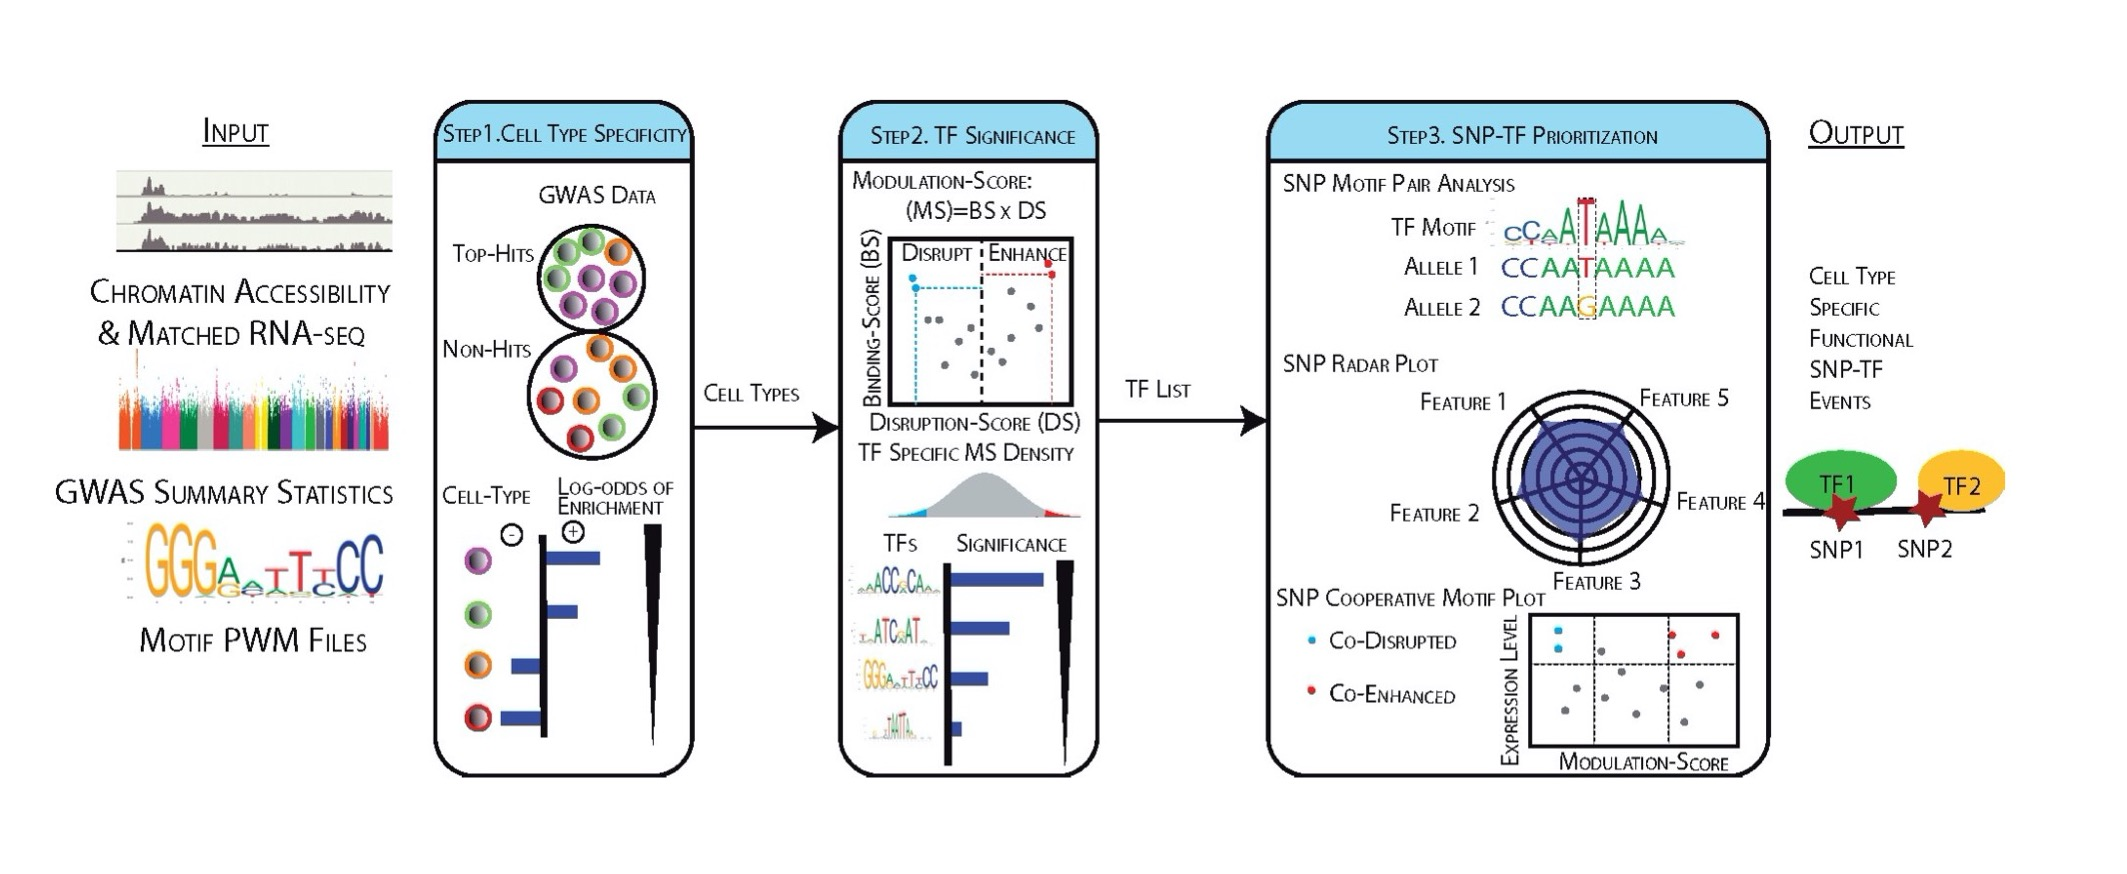
\includegraphics[width=\textwidth]{figures/motifraptor1.jpg}
	\caption[MotifRaptor analysis workflow]{\textbf{MotifRaptor analysis workflow.} Three steps are performed: (1) characterize
relevant cell types based on the enrichment of phenotype associated SNPs in chromatin accessible
sites, (2) find TFs with binding sites that are significantly modulated by genetic variants in these
cell types and (3) identify and visualize individual TF-SNP regulation events}
	\label{fig:motifraptor1}
\end{figure} 
% - Quantifying the genetic variants effects on TF binding sites
\subsubsection{Quantifying the genetic variants effects on TF binding sites}
To assess the impact of genetic variants at a certain TF binding site,, \motifraptor implements an efficient genome-wide and threshold-free scoring procedure, scanning all the binding sites overlapping the target variants. Given a genomic sequence $s$, where $|s|=m$, and a position weight matrix (PWM), the score $M(i,S_{i})$ indicates the likelihood of observing the nucleotide $S_{i}\in\{A,C,G,T\}$ at position $i$, where $1 \leq i \leq m.$ We derive the binding score $BS$ from $M(i,S_{i})$ as a log-likelihood score computed over the entire binding site and corrected to account for genome-wide nucleotide frequencies, or background frequencies, $B(s_{i})$:
\[
	BS = \log{\prod^{m}_{i=1}{\frac{M(i,s_{i})}{B(s_{i})}}} = \sum^{m}_{i=1}{(\log{M(i, s_{i}))} - \log{B(s_{i})})}
\] 
from this formulation, \motifraptor derives a disruption score $DS$, capturing the potential impact of genetic variants on a given binding site. Given a target variant, \motifraptor assumes two haplotypes, denoted by $s_{ref}$ and $s_{alt}$, for the reference and alternative alleles, respectively. \motifraptor scores each allele to obtain the binding score for the reference and alternative alleles (i.e.  $BS(s_{ref})$ and $BS(s_{alt})$). For scalability reasons it limits the computations to a region spanning 61 bp, centered around the target variant. For each region \motifraptor considers the best putative binding position $K$ for both $s_{ref}$ and $s_{alt}$:
\[
	K = \argmax_{1 \leq k \leq m}(BS(s_{ref, k:k+m-1}, M), BS(s_{alt, k:k+m-1}, M))
\]
Therefore, the disruption score at K is defined as:
\[
	DS = \Delta BS
\]
The value and sign of the $DS$ become informative indicators on the directionality and strength of the target variant impact on TF binding. In fact, positive $DS$ indicate enhanced binding affinities, while negative values a reduced binding potential. Since different TF binding site motifs have diverse length and specificities, \motifraptor rescales both the $BS$ and $DS$ in $[0,1]$ and $[-1,1]$, respectively. Given the rescaling of the two scores, \motifraptor defined a Binding-Disruption (BD) space to visualize and summarize the TF-SNP modulation events globally and across different factors.
% -- Assessing TF-SNP modulations significance
\subsubsection{Assessing TF-SNP modulations significance}
To quantify the significance of the predicted TF-SNP modulation events prioritized, \motifraptor employed a method based on the central limit theorem (CLT). Therefore,  estimated a complete null-model based on the enumeration of all potential binding sites on the genome. To maintain the scalability, \motifraptor employed advanced sequence data structures like Suffix Arrays and Longest Common Prefix Arrays. These data structures allow the exhaustive enumeration keeping the method scalability.  Given a set of target variants $T$, to assess if they significantly modulate TF binding events, \motifraptor tests whether the B-S space significantly differed from the B-S space obtained from a set of background SNPs $B$.  To assess the difference between the distributions \motifraptor uses a non-parametric test with null hypothesis $E(D_{B-S_{space}}(T))=E(D_{B-S_{space}}(B))$. Since based on the CLT, the distribution of the sample mean of $B$ converges to a normal distribution, its mean and variance are equal to $E(D_{B-S_{space}}(B))$ and $\frac{\Var(D_{B-S_{space}}(B)}{N_{samples}}$,  regardless of the underlying B-S space values distribution. Therefore, \motifraptor tests the significance of both the enhanced binding $((D_{B-S_{space}}(T)) > E(D_{B-S_{space}}(B)))$, disrupted binding $((D_{B-S_{space}}(T)) < E(D_{B-S_{space}}(B)))$, or both. This procedure combined with efficient data structures allows to identify significant genome-wide shifts in TF-SNP binding modulations without using predetermined scores or cutoff on $p$-values.
% -- Improving MotifRaptor by employing SVM-based motif models
\subsection{Improving MotifRaptor by employing SVM-based motif models}
In the case study presented in the original paper, \motifraptor's predictions were supported by literature, suggesting that it leverages promising ideas. However, \motifraptor’s main limitation is the employed computational models to represent TF binding motifs. Despite position weight matrices \citep{stormo2000dna} (PWMs) are simple, intuitive, and widely employed TF motif models, PWMs carry several drawbacks that often result in under- or over-estimation of non-coding variant impact on TFs binding landscape \citep{tognon2023survey}. TF SVM-based motif models \citep{tognon2023survey, boeva2016analysis} have been demonstrated to overperform PWMs in several tasks, such as prediction of binding events and variants impact on TF binding sequences. However, while several publicly available resources provide complete and extensive collections of motif PWMs, to our knowledge there is no complete collection of SVM-based TF motifs. Therefore, we propose an extensive and curated collection of SVM-based motifs as well as a novel approach to annotate the functional impact of non-coding variants on TF binding landscape using SVM-based models, which interpolates different omics data, such as transcriptome, DNase-seq \citep{john2011chromatin}, ATAC-seq \citep{buenrostro2013transposition}, etc. 
% - Building a library of transcription factor SVM-based models
\subsubsection{Building a library of transcription factor SVM-based models}
SVM-based models have demonstrated superior performance compared to traditional PWMs \citep{tognon2023survey}. However, a significant drawback persists as no motif database currently offers these advanced SVM-based models. Moreover, the interpretability of these models remains a challenging issue, and there is a scarcity of motif analysis tools that harness the power of SVMs-based motif models. To address these limitations,  we propose the creation of a comprehensive library comprising SVM-based motif models. To compute the SVM-based motif models we use ChIP-seq data from ENCODE \citep{encode2012integrated}.  To enhance model reproducibility, we modified FactorBook's model computation pipeline \citep{pratt2022factorbook} (\textbf{Fig.\ref{fig:motifraptor3}}).
\begin{figure}
	\centering
	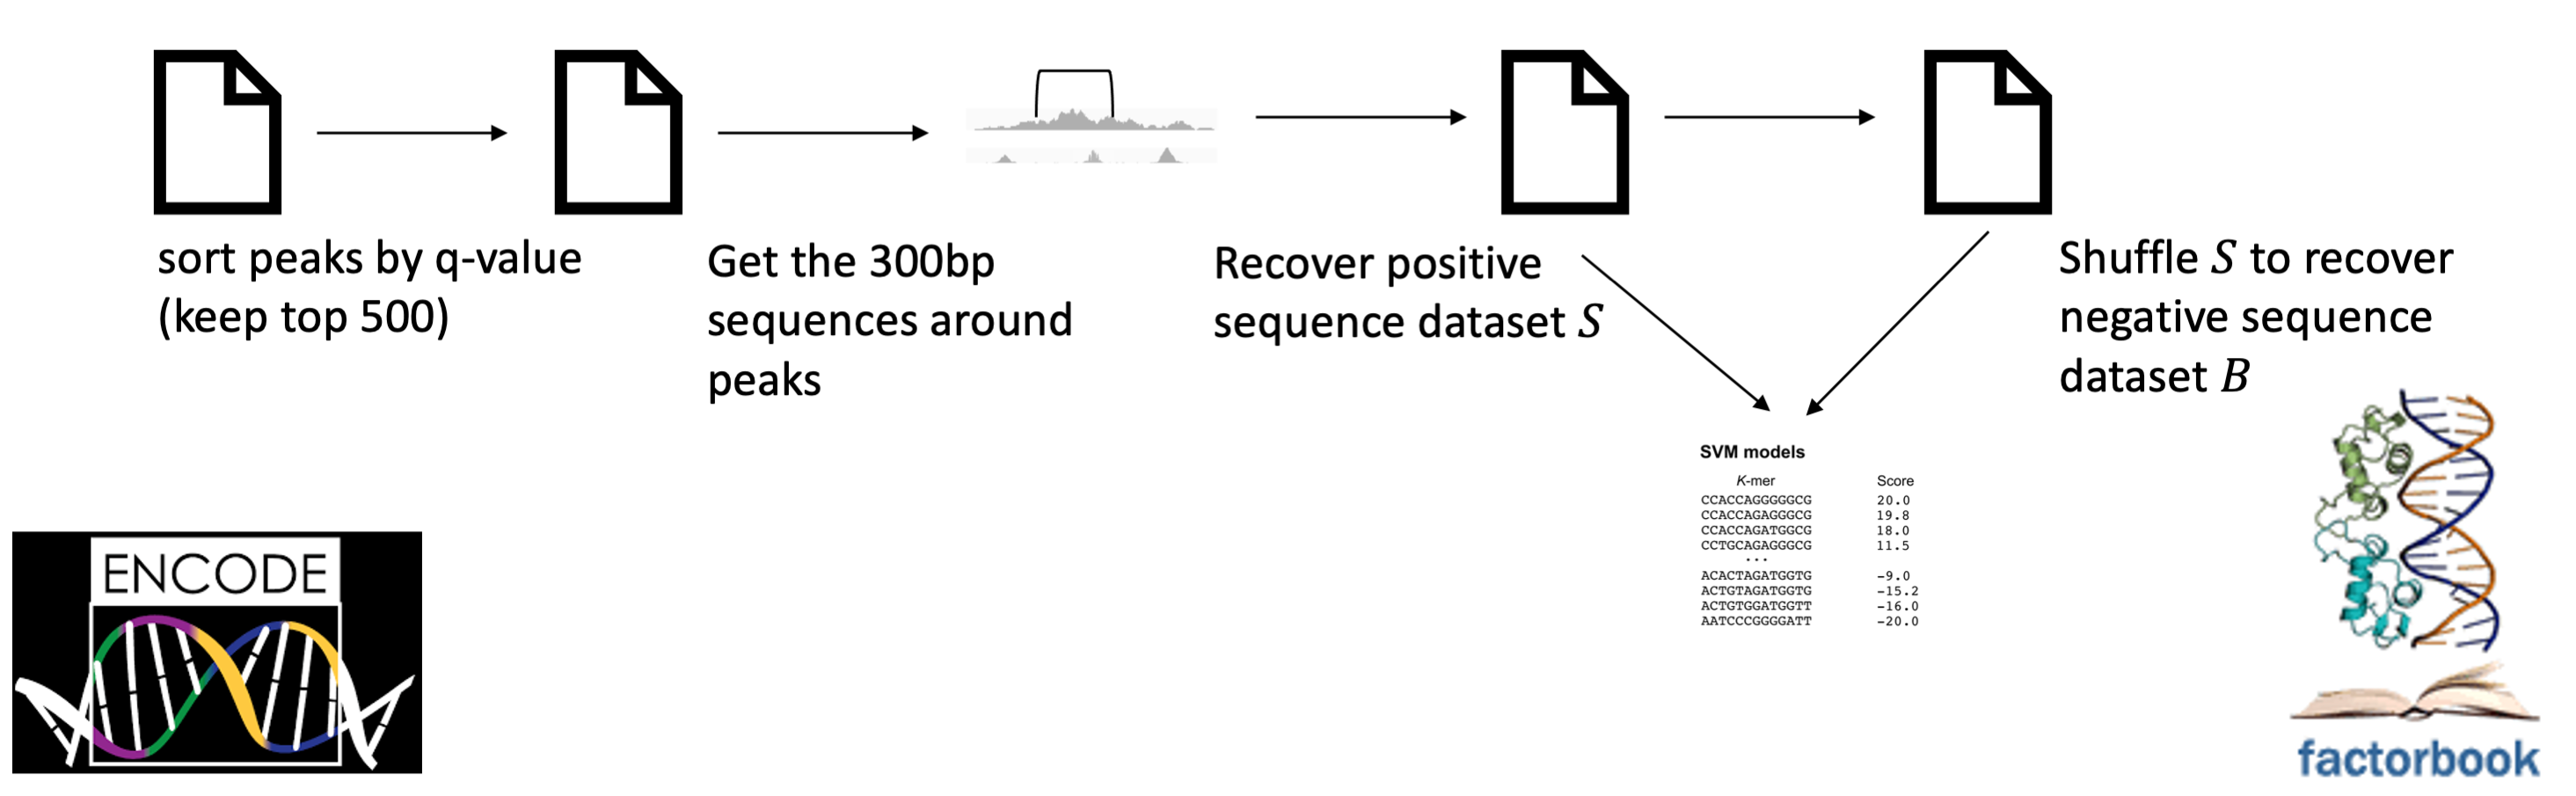
\includegraphics[width=\textwidth]{figures/motifraptor3.png}
	\caption[SVM-based motif models computation workflow]{\textbf{SVM-based motif models computation workflow.} For the sake of reproducibility, we follow the model computation pipeline employed by FactorBook database, to derive PWM models from ENCODE data.}
	\label{fig:motifraptor3}
\end{figure} 
To compute the models we selected ChIP-seq peaks datasets from ENCODE retrieved on different tissues and cell types.  For each ChIP-seq dataset, we selected the top 500 peak sequences sorted by $q$-value. Then, we shrinked the surviving peaks to 300 bp centered around the peak signal center. After recovering the resulting genomic sequences, we constructed a background dataset by shuffling the original sequences. The two dataset are, then, used as input to compute the SVM models using LS-GKM \citep{lee2016ls}.
% - Comparing SVM-based and PWM motif models predictive power
\subsubsection{Comparing SVM-based and PWM motif models predictive power}
\begin{figure}
	\centering
	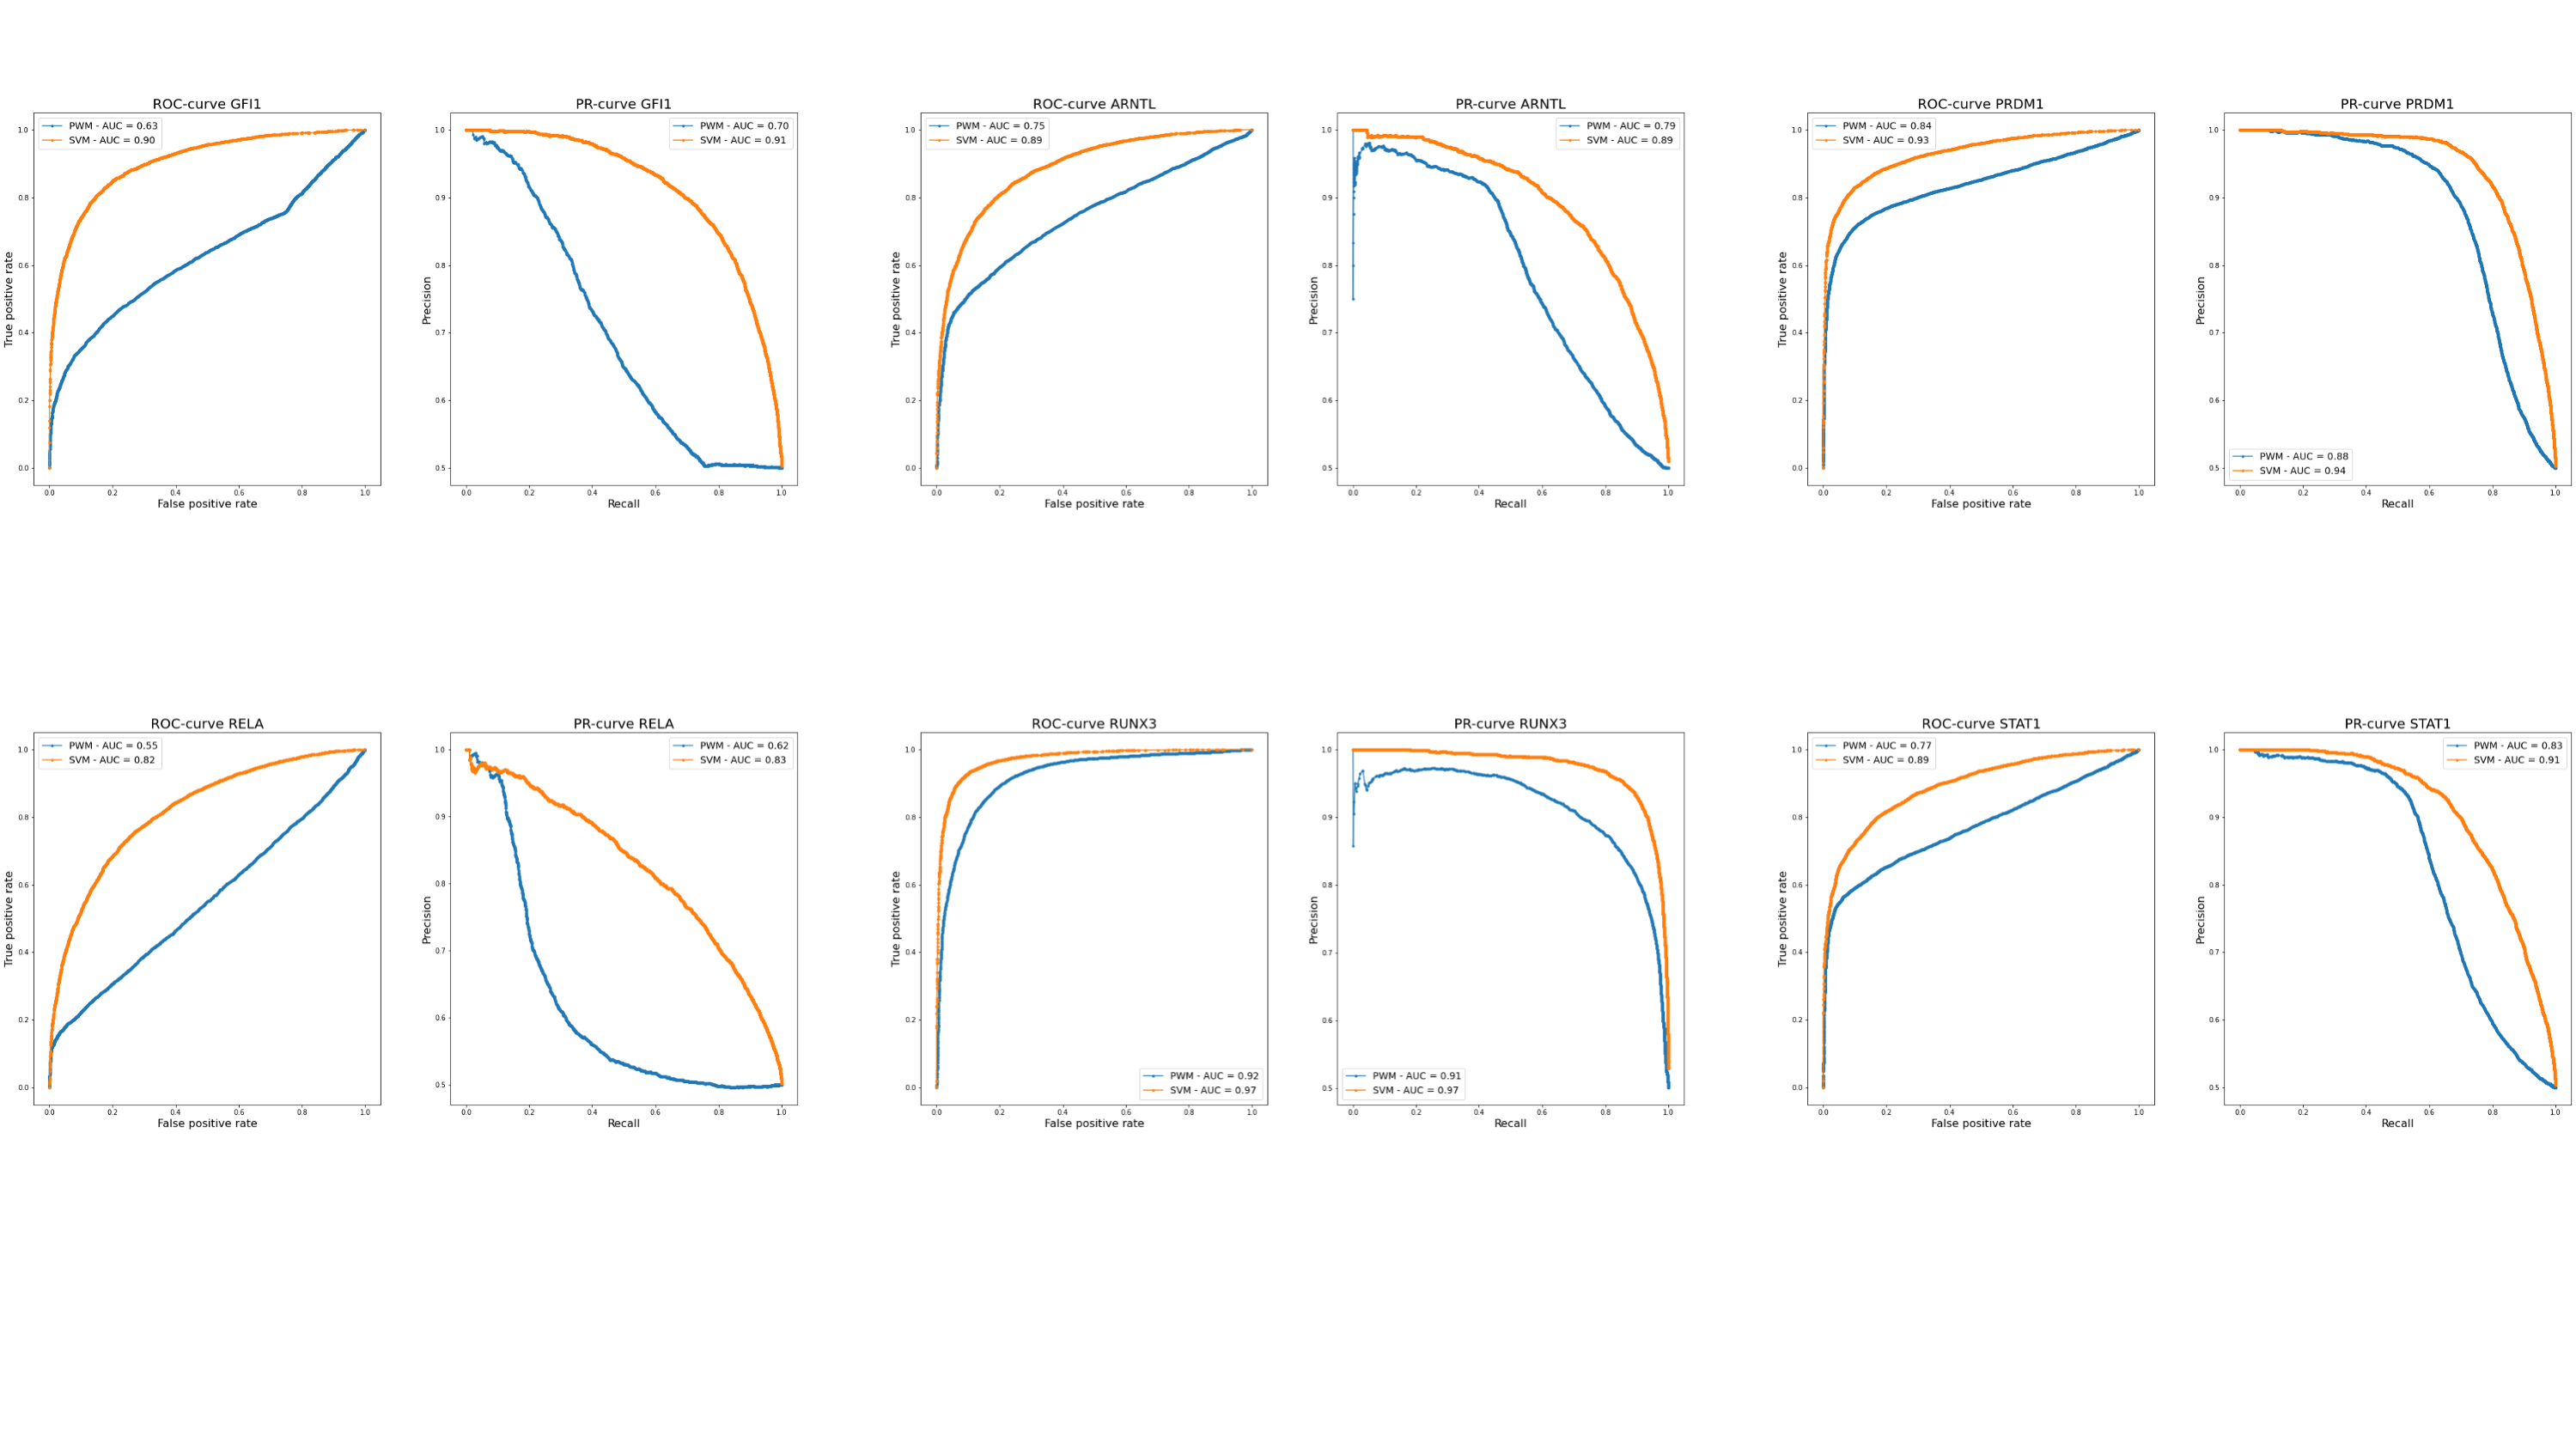
\includegraphics[width=\textwidth]{figures/motifraptor2.png}
	\caption[Comparing SVM-based and PWM motif models predictive power]{\textbf{Comparing SVM-based and PWM motif models predictive power.} We compared the predictive power of SVM-based and PWM motif models for six transcription factors: ARNTL, GFI1, PRDM1, RELA, RUNX3 and STAT1. Both models were trained on ENCODE ChIP-seq data (cell line GM12878). To train SVM-based models we followed the described pipeline, while to train PWM models we replaced LS-GKM with MEME. The predictive perfomance of the two models have been compared computing ROC- and PR-curves.}
	\label{fig:motifraptor2}
\end{figure} 
We demonstrate the improvements brought by SVM-based motif models over PWMs, by comparing the predictive power of the two models in terms of ROC- and PR-curves. For this analysis we selected the six TFs that have been previously identified in the original \motifraptor publication to be affected by mutations linked to rheumatoid arthritis: ARNTL, GFI1, PRDM1, RELA, RUNX3, and STAT1. For the assessment we employed the original and the modified FactorBook pipeline, where the latter replaces MEME with LS-GKM to compute the SVM models. MEME \citep{bailey1994fitting} is a widely used software to compute PWM motif models from sequence data. To train and test the models we selected one ChIP-seq dataset for each TF (GM12878 cell line) from the ENCODE data portal. After training, we compared models' performance via a $4$-fold cross-validation (75\% training and 25\% testing) on the top 500 peaks, selected following FactorBook's pipeline. By running our comparison, we observed that generally SVM-base motif models better predict binding events than PWMs, in both terms of ROC and PR-curves (\textbf{Fig.\ref{fig:motifraptor2}}).
% -- Future directions
\subsection{Future directions}
In the next future we plan to complete our SVM-based motif models catalog extending the presented analysis to all the remaining TFs whose ChIP-seq data are available in ENCODE. Additionally, ENCODE datasets could be integrated employing datatasets from different databases, such as Cistrome \citep{zheng2019cistrome} or GTRD \citep{kolmykov2021gtrd}. Moreover, we plan to release to the community the complete SVM motif models catalog. We also plan to train models on SELEX data rather than ChIP-seq and compare the resulting models. Importantly, since SELEX is a method less susceptible to noise than ChIP-seq the resulting models could potentially provide an even larger boost of models' predictive performance. We plan to modify \motifraptor scanning algorithm for both PWM and SVM motif models to consider haplotypes, and indels. In fact,  currently \motifraptor consider only SNP and treats them as independent events, however it is known that complex SNP-SNP, SNP-indel, indel-indel combination can happen \citep{tognon2021grafimo}, often with signifcant effects on TF binding potential.
% ------ CRISPR off-targets
\mychapter{6}{CRISPR genome editing}
CRISPR genome editing \citep{cong2013multiplex} has revolutionized genetic engineering, allowing for precise modifications in the genomes of living organisms. CRISPR offers a versatile and programmable approach, linking coupling binding to genomic target sequences with diverse effector proteins, restricted by protospacer adjacent motif (PAM) sequences.  By delivering the Cas9 nuclease complex coupled with a synthtic guide RNA (gRNA), into a cell CRISPR provides a simple and programmable means to modify genomic sequences at specific locations, enabling the addition or removal of genes \emph{in vivo}. Significantly, CRISPR opens up unprecedented opportunities for developing novel therapies by introducing precise genetic or epigenetic modifications to targeted genomic regions. The precision of CRISPR-Cas9 editing hinges on two crucial factors: (i) the target sequence, a 20 bp string within each CRISPR locus of the gRNA array \citep{ran2013genome}, which typically has multiple unique targets, and (ii) the PAM sequence, short nonspecific sequences scattered throughout the genome \citep{ran2013genome}, which Cas9 identifies to initiate editing. Once the requisite sequences are assembled, Cas9 locates its target on the genome under the guidance of the gRNA. The Cas9 nuclease opens both strands of the genomic target, to introduce novel and precise modifications. Cas9 operates primarily through two mechanisms: (i) knock-in and (ii) knock-out mutations,(\textbf{Figure \ref{fig:crispr}}). In knock-in, homology-directed repair (HDR) employs DNA sequences that resemble the target to mend the Cas9-induced breaks in the genome, using exogenous DNA as a template for repair. It is essential to note that this method relies on specific and isolated damaged sites within the target region to initiate DNA repair processes. Conversely, in knock-out, the mutations in the DNA introduced by Cas9 result in the repair of breaks via nonhomologous end joining (NHEJ). Repair through NHEJ often leads to random insertions and deletions in the target sequence, which can disrupt, enhance, or alter the function of the targeted site.
\begin{figure}
	\centering
	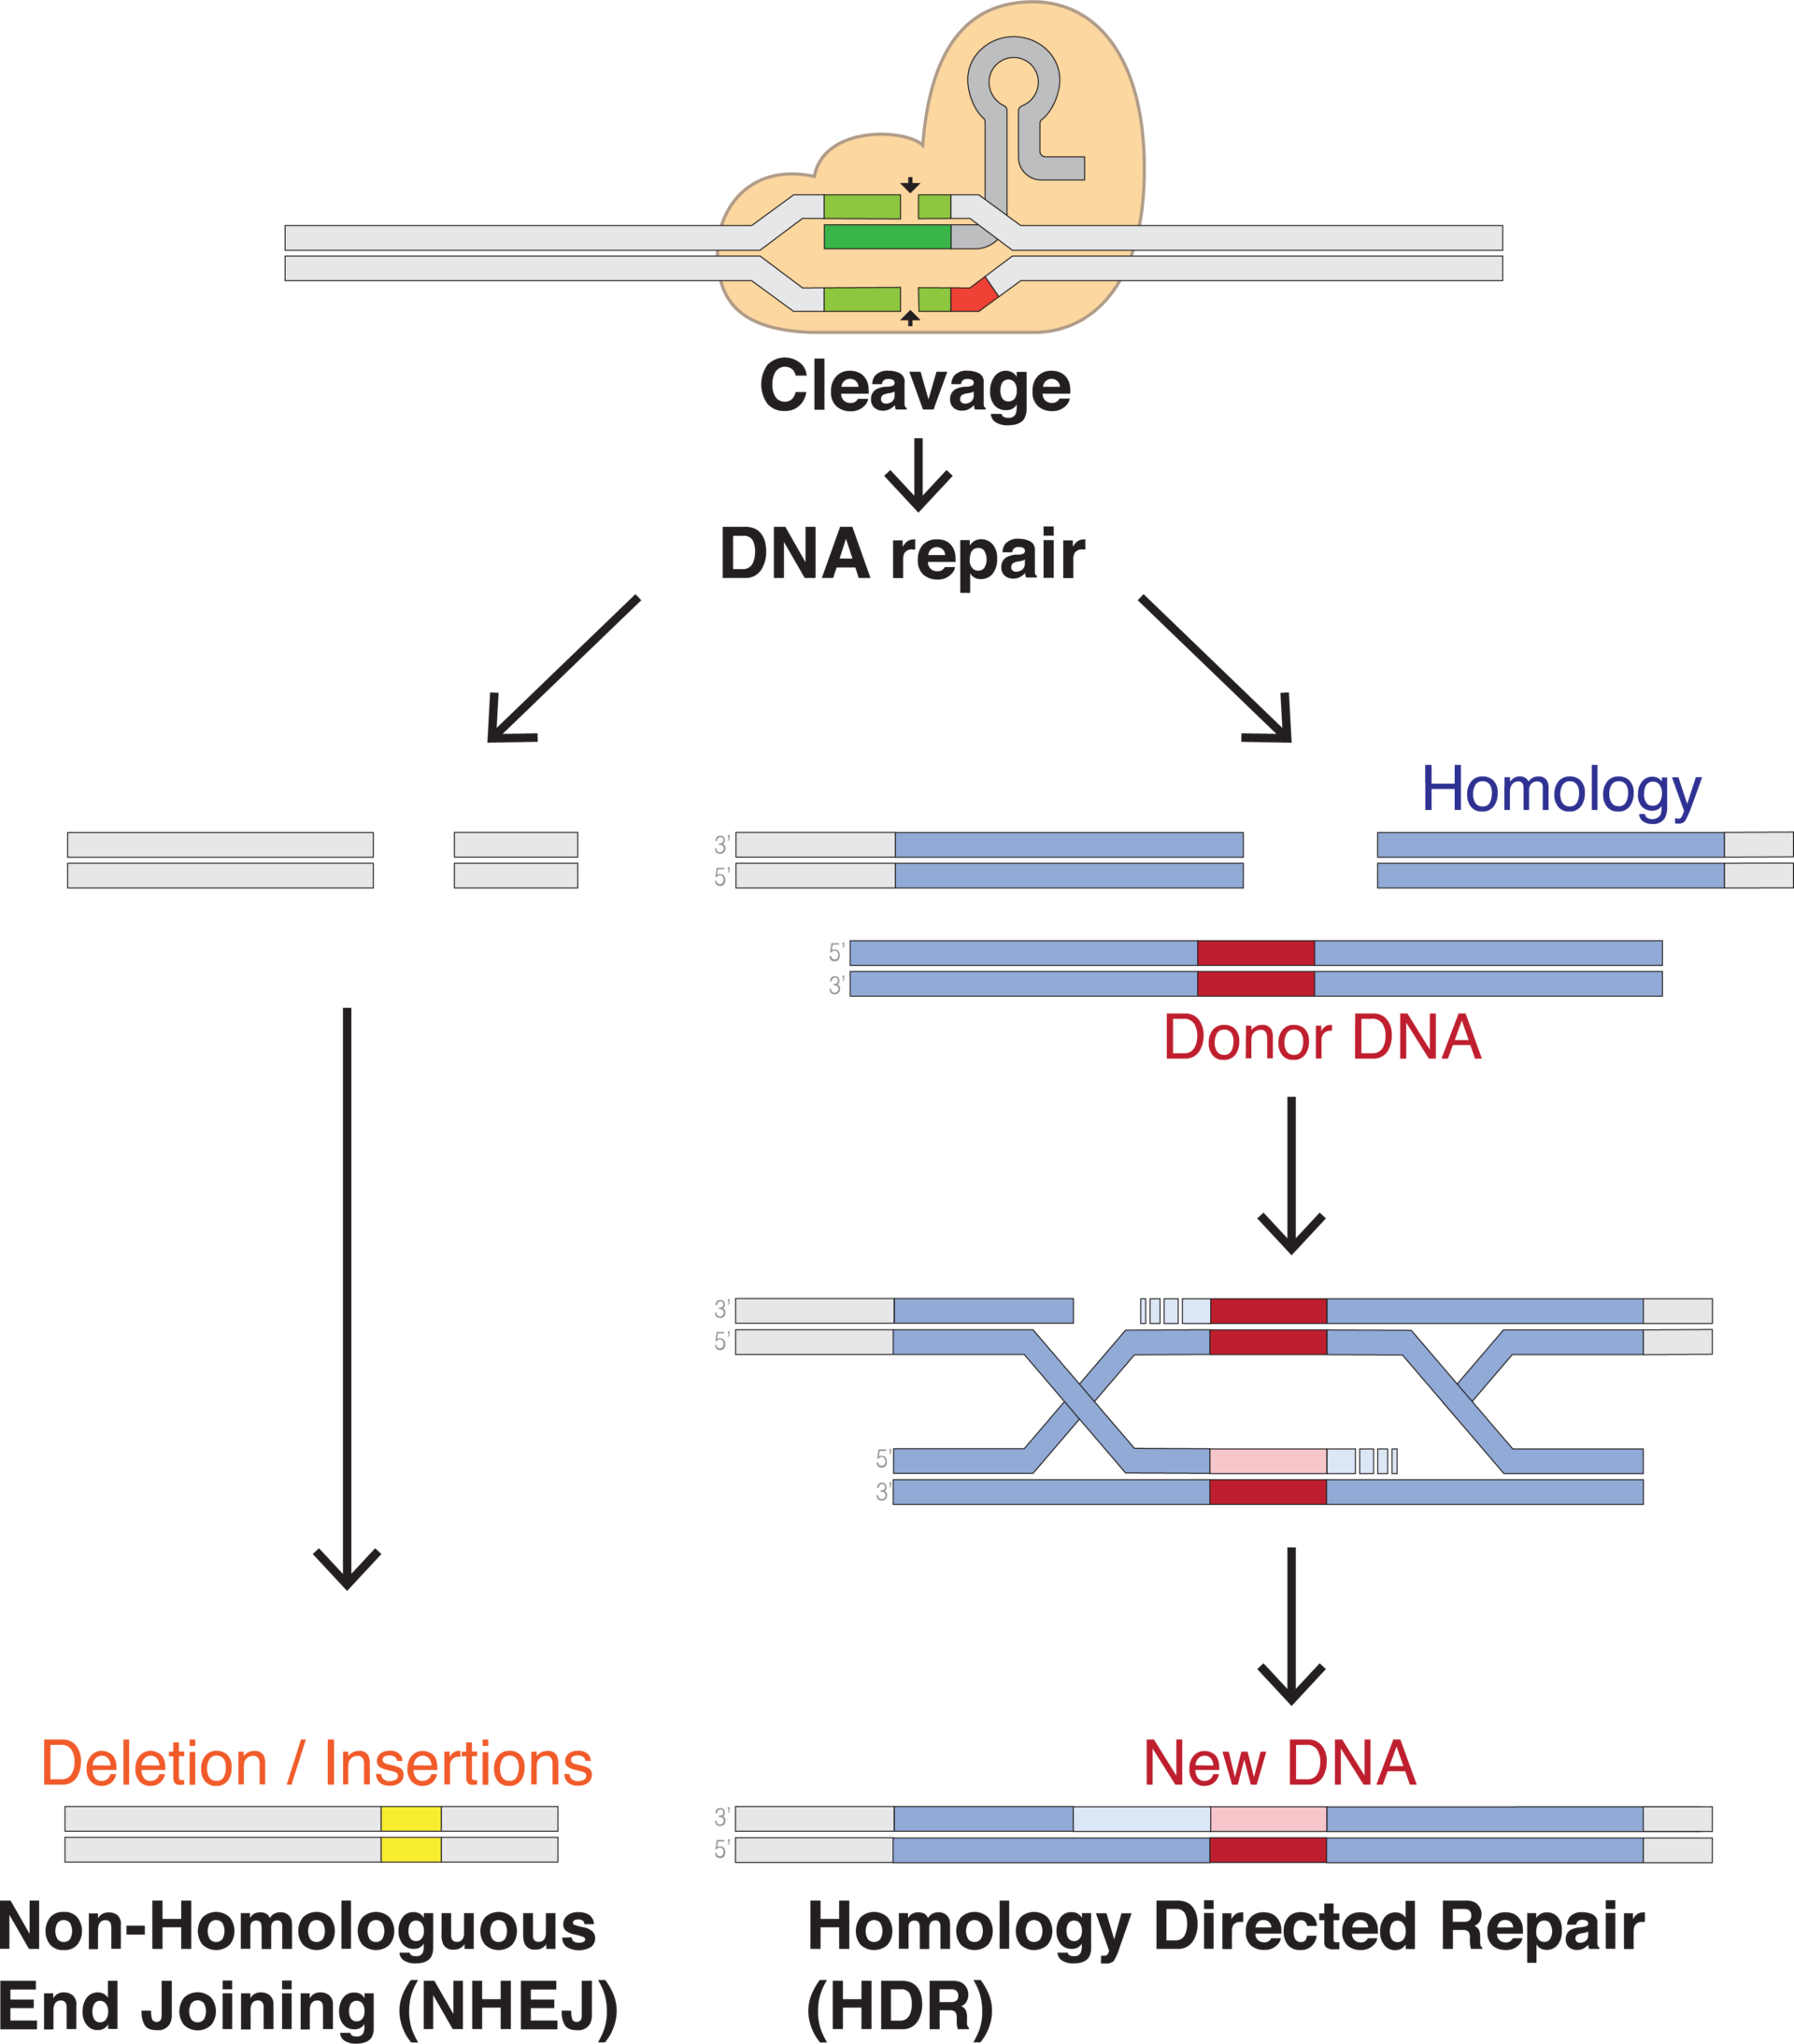
\includegraphics[width=\textwidth]{figures/crispr.png}
	\caption[CRISPR gene editing via HDR and NHEJ]{\textbf{CRISPR gene editing via HDR and NHEJ.}}
	\label{fig:crispr}
\end{figure} 
Given that CRISPR-Cas9 empowers precise yet potentially random gene disruption, the meticulous design of guide RNAs (gRNA) to effectively steer Cas9 toward the intended target sequence (\emph{on-targets}) is of paramount importance. This precision is essential to prevent unintended and potentially hazardous alterations in non-targeted sequences (\emph{off-targets}). Moreover, genetic variants can potentially modify target and PAM sequences, thereby impacting both on-target and off-target potentials. Consequently, when crafting gRNA designs, it becomes imperative to account for genetic diversity, particularly in clinical settings, in order to avert possible undesired and hazardous consequences within the host genome.
% ---- Benchmarking whole genome sequencing to detect CRISPR genome editing events
\section{Benchmarking whole genome sequencing to detect CRISPR genome editing events}
One of the major hurtles for the clinical adoption of CRISPR genome editing technologies is the risk of genome editing at unpredicted genomic sites \citep{fu2013high}. Computational and experimental strategies have been developed to nominate off-target editing sites \citep{clement2020technologies}. ). In practice, these nomination strategies produce a ranked list of sites, of which the top hits are prioritized for validation using amplicon sequencing to quantify evidence of genome editing\citep{akcakaya2018vivo}. However, nomination strategies have an arbitrary cutoff or no cutoff to distinguish which sites should be experimentally validated, and the number of sites chosen for validation are sometimes selected subjectively based on budget or choosing nice round numbers (e.g. the top 100). Unfortunately, the possibility of editing at nominated sites lower down the prioritized list-combined with the possibility that the nomination strategies may not comprehensively capture the genome editing dynamics of actual CRISPR genome editing–have led many to suggest that reliance on nomination strategies may be insufficient to exclude editing at unpredicted sites.  Whole-genome sequencing (WGS) has been proposed as a standard to comprehensively examine the genome for evidence of genome editing. WGS has several benefits, including the ability to potentially measure genome editing activity at every base in the genome, and to measure complex genome editing outcomes such as translocations. However, despite increased availability and reduced cost of genome sequencing, WGS remains an expensive proposition as significant sequencing of the entire genome must be performed to detect rare editing events, and it is difficult to distinguish rare editing events from sequencing errors. WGS has been used to detect genome editing events in clonal cell lines \citep{smith2014whole, veres2014low} where individual cells within a clone serve as replicates to reduce bias of sequencing artifacts. However, this method is inadequate for use in detecting rare off-targets because the limit of detection is based on the number of clones (e.g. WGS of 100 clonal lines would need to be performed to detect an editing event at a 1/100 (1\%) rate). 
To investigate the utility of WGS as a method to detect genome editing events genome-wide in bulk populations, we have created models for the sequencing depth required for detection of editing events. We have produced ultra-deep 1000x WGS datasets of genome-edited samples and used them to characterize editing at on- and off-target sites, and compare editing detection in WGS to several experimental nomination and computational detection methods. We then propose an unbiased genome editing detection method which can identify the genome editing from WGS data in cases when the CRISPR guide sequence is not known. Together, these models, datasets, and methods provide an assessment of the utility for whole genome sequencing in the detection of genome editing. 
% -- Modeling sequencing depth requirements to detect genome editing
\subsection{Modeling sequencing depth requirements to detect genome editing}
The actual problem of detecting genome editing can be broken into two parts: (i) sequencing genomic DNA with sufficient depth to detect editing at a given site, and (ii) correctly interpreting the sequencing data (e.g. read alignment and variant calling) to discriminate true CRISPR edits from technical noise. We address the first question regarding sequencing depth using a binomial model, and use simulated samples to measure the ability of existing mutation callers to detect edited genome-edited reads as such.
DNA sequencing for the detection of editing events can be performed in a heterogenous population of edited cells with a detection limit and detection power proportional to the sequencing depth. This approach to determining sequencing depth requirements applies to amplicon sequencing of a single locus as well as to whole-genome sequencing. We note that WGS can be performed at low coverage on clonal lines to detect genome editing in single cells, but in this case the limit of detection is defined based on the number of single cell clones that can be sequenced. To detect genome editing – especially rare editing events – in cell populations, samples must be sequenced with sufficient depth, meaning that the sequence of sufficiently many DNA molecules must be read in order to find one containing an editing event. To measure rarer editing events, deeper sequencing must be performed. We used a statistical model to formalize the power to recover editing events at varying frequencies based on the binomial distribution \citep{petrackova2019standardization}. Using this model we can calculate the sequencing depth required to observe a certain number of reads given a frequency of edited reads in a sample. For example, 30 reads are required to detect a single edited read in a sample with a mutation rate of 10\% and 300 reads are required to detect a single edited read in a sample with a mutation rate of 1\% at 95\% power, or that in 95\%. We can also use the binomial distribution confidence interval to calculate the range of true editing rates given an observed editing rate and sequencing depth. For example, the 95\% confidence interval for an edit in 15/30 reads is between 31.3\% and 68.7\%. In order to assess the ability of mutation callers to detect genome editing events, we created simulated samples by inserting mutations found in reads from amplicon sequencing of 14 on- and off-targets from Fu \emph{et al}. \citep{fu2014improving} into whole-genome sequence from the Genome in a Bottle Consortium \citep{zook2016extensive}. We plan to measure the ability of three commonly-used mutation callers to recover simulated reads resulting from genome editing \citep{mckenna2010genome, kim2018strelka2, koboldt2012varscan}.
% -- Generation of WGS datasets
\subsection{Generation of WGS datasets}
Whole-genome sequencing is commonly performed to identify mutations genome-wide, and has been applied in clinical settings to detect disease-associated germline mutations \citep{thiffault2019clinical}. Clinical whole-genome sequencing aims for 30x-50x coverage of samples, and 40x coverage has been reported to provide sufficient depth to detect heterozygous and homozygous SNPs \citep{sun2021characterizing}. According to our model introduced above, sequencing at 30x can detect one edited read in the context of approximately 5\% genome editing at 80\%. In order to detect rarer editing events, deeper sequencing must be performed. We aimed to create whole genome sequencing libraries at 1000x, which should be able to detect one edited read with a 0.2\% editing rate with 80\% power.  We performed genome editing in K562 and GM12878-Cas9 cell lines \citep{ma2017crispr} with four guides with varying specificities as measured by the number of sites in the genome with sequence homology with up to 4 mismatches. We selected RNF2 (precise guide, 7 off-by-4 sites), EMX1 (mid specificity, 293 off-by-4 sites), HEKSite4 (mid specificity, 832 off-by-4 sites), and VEGFASite3 (promiscuous, 6509 off-by-4 sites). Additionally we used a Cas-12a guide targeting DNMT1Site3 as a control guide. For each sample we prepared PCR-free sequencing libraries. Genomic sequencing depth was measured using Mosdepth \citep{pedersen2018mosdepth}, and showed a minimum of 89\% genomic coverage at 1000x in GM12878 and at least 57\% genomic coverage at 1000x in K562.
% -- Measurement of editing using existing tools
\subsection{Measurement of editing using existing tools}
We used our WGS samples to test the ability to identify edited bases by existing tools which are used for variant calling in non-CRISPR settings. Although these tools have been developed to disregard technical artifacts such as sequencing errors, and some have been developed to detect rare alleles, none have been developed to identify CRISPR-edited reads or genomic sites of CRISPR editing. We therefore tested the ability of these tools to detect CRISPR editing at and around sites nominated by experimental (GUIDE-seq \citep{tsai2015guide}, CIRCLE-seq \citep{tsai2017circle}), and computational (Casoffinder \citep{bae2014cas}) methods.  For each nominated region, we defined a region within 100bp of the predicted cutting location where we would expect to see CRISPR editing. We also defined 10Kb windows up- and downstream from the nominated region (not including the 100bp window) where we did not expect to see editing. We used Mutect \citep{mckenna2010genome}, Varscan \citep{koboldt2012varscan},  and Strelka \citep{kim2018strelka2} were used to identify variants for each nominated region, and classified variants within the 100bp window as true-positives and variants in the 10kb flanking windows as false-positives. 
% -- Enhancement of off-target editing detection by predictive models
\subsection{Enhancement of off-target editing detection by predictive models}
Our WGS dataset provides the benefit of being able to investigate editing across the genome without knowing beforehand the sites to be investigated – albeit at a depth of around 1000x coverage. This is in contrast to strategies such as amplicon sequencing where much greater depth can be achieved but the genomic sites to be amplified must be selected in advance, and editing cannot be investigated outside the selected regions. We have capitalized on this characteristic of our WGS dataset and identify nuclease effects at a variety of regions. We used Casoffinder to identify all putative cut sites with up to 4 mismatches and 1 bulge with respect to the guide sequence, and used CRISPRessoWGS \citep{clement2019crispresso2} to calculate the percentage of reads with indels in the treated and control sample.
% -- Unbiased detection of genome editing targets
\subsection{Unbiased detection of genome editing targets}
Next, we sought to identify sites of genome editing, but without relying on knowing the sgRNA sequence used to edit the sample. This unbiased approach is valuable because it allows detection of CRISPR edits in a sample where the sgRNA was not known, and it can also be used to find CRISPR edits that may occur at locations without sequence similarity to the sgRNA. We note that many experimental nomination methods constrain reported hits to sites with homology to the sgRNA sequence because naturally occurring double-strand breaks frequently occur at fragile or AT-rich genomic sites \citep{nobles2019iguide}, ), so an unbiased method using WGS could identify guide sequence-independent editing events.  Unfortunately, WGS data contains noise from different sources that makes it difficult to identify genome editing. These sources of noise include sequencing errors, alignment errors, and allelic diversity. We developed an unbiased genome editing discovery algorithm that attempts to discriminate between sites of CRISPR editing and noise by comparing a treated sample to a control sample because we expect that these sources of noise will affect the control sample as well as the treated sample. In addition, we exploit two additional characteristics of genome editing: High rates of insertions/deletions at the on-target and diversity of editing at the on-target – we expect that more than one allele will be produced as the result of stochastic double-strand break repair after Cas9 editing. We ran our unbiased algorithm to detect ranked sites of editing in all WGS samples. The ranking of sites with putative editing correlates well between the GM12878 and K562 cell lines, suggesting that the majority of editing is reproducible across cell types. We observe slightly more sensitivity in the K562 line for detecting off-target sites nominated by CIRCLE-seq. This is likely be due to the higher editing rates in the K562 cell line. Importantly, our unbiased algorithm identifies the on-target edit site among the top hits in all guides and in both cell lines.
% ---- CRISPRme
\section{\crisprme}
CRISPR genome editing offers extraordinary opportunities to develop novel therapeutics by introducing targeted genetic or epigenetic modifications to genomic regions of interest. Briefly, CRISPR provides a simple and programmable platform that couples binding to a genomic target sequence of choice with diverse effector proteins through RNA:DNA (spacer:protospacer) complementary sequence interactions mediated by a gRNA spacer sequence matching a genomic protospacer sequence restricted by PAM sequences. Editing effectors may consist of nucleases to introduce targeted double strand breaks leading to short insertions/deletions (indels) and templated repairs (for example, Cas9), deaminases for precise substitutions (base editors) or chromatin regulators for transcriptional interference or activation (CRISPRi/a), among others, to achieve a range of desired biological outcomes \citep{anzalone2020genome}. CRISPR-based systems may create unintended off-target modifications posing potential genotoxicity for therapeutic use. Several experimental assays and computational methods are available to uncover or forecast these off-targets \citep{clement2020technologies}. Off-target sites are partially predictable based on homology to the spacer and PAM sequence. Beyond the number of mismatches or bulges, a variety of sequence features, like position of mismatch or bulge with respect to PAM or specific base changes, contribute to off-target potential \citep{clement2020technologies, bao2021tools, hsu2013dna, doench2016optimized}. Computational models can complement experimental approaches to off-target nomination in several respects: to triage gRNAs before experiments by predicting the number and cleavage potential of off-target sites and to prioritize target sites for experimental scrutiny. Genetic variants may alter protospacer and PAM sequences and therefore may influence both on-target and off-target potential. Gene editing strategies designed to specifically recognize patient mutations may increase the likelihood of editing mutant alleles, whereas variants that reduce homology to the anticipated target may decrease the efficiency of the desired genetic modification. Although a variety of in vitro and cell-based experimental methods can be used to empirically nominate off-target sites, these methods either use homology to the reference genome as a criterion to define the search space and/or use a limited set of human donor genomes to evaluate off-target potential \citep{bao2021tools, chaudhari2020evaluation}. Therefore, computational methods may be especially useful to predict the impact of off-target sequences not found in reference genomes. Prior studies considering gRNAs targeting therapeutically relevant genes using population-based variant databases like the 1000 Genomes Project (1000 G) and the Exome Aggregation Consortium have highlighted how genetic variants can substantially alter the off-target landscape by creating novel and personal off-target sites not present in a single reference genome \citep{lessard2017human, scott2017implications}. Although these prior studies provide code to reproduce analyses, implementation choices make these tools not suitable to analyze large variant datasets and to consider higher numbers of mismatches. In addition, these methods ignore bulges between RNA:DNA hybrids, cannot efficiently model alternative haplotypes and indels, and require extensive computational skills to utilize. Several user-friendly websites have been developed to aid the design of gRNAs and to assess their potential off-targets \citep{concordet2018crispor, listgarten2018prediction, labun2019chopchop, park2015cas}. Even though variant-aware prediction is an important problem for genome editing interventions, these scalable graphical user interface (GUI) based tools do not account for genetic variants. In addition, these tools artificially limit the number of mismatches for the search and/or do not support DNA/RNA bulges. Therefore, designing gRNAs for therapeutic intervention using current widely available tools could miss important off-target sites that may lead to unwanted genotoxicity. A complete and exhaustive off-target search with an arbitrary number of mismatches, bulges, and genetic variants that is haplotype-aware is a computationally challenging problem that requires specialized and efficient data structures.We have recently developed a command line tool that partially solves these challenges called CRISPRitz \citep{cancellieri2020crispritz}. This tool uses optimized data structures to efficiently account for single variants, mismatches and bulges but with substantial limitations Here, we substantially extend this work by developing \crisprme, a tool to aid gRNA design with added support for haplotype-aware off-target enumeration, short indel variants and a flexible number of mismatches and bulges \citep{cancellieri2023human}. \crisprme is a unified, user-friendly web-based application that provides several reports to prioritize putative off-targets based on their risk in a population or individuals. \crisprme is flexible to accept user-defined genomic annotations, which could include empirically identified off-target sites or cell-type-specific chromatin features. The tool can integrate population genetic variants from sets of phased individual variants (like those from 1000 G \citep{lowy2019variant}), unphased individual variants (like those from the Human Genome Diversity Project (HGDP) \citep{bergstrom2020insights}) and population-level variants (like those from the Genome Aggregation Database (gnomAD) \citep{karczewski2020mutational}).  Furthermore, it can accept personal genomes from individual subjects to identify and prioritize private off-targets due to variants specific to a single individual. Here, we demonstrate the utility of \crisprme by analyzing the off-target potential of a gRNA currently being tested in clinical trials for sickle cell disease (SCD) and $\beta$-thalassemia \citep{frangoul2021crispr, canver2015bcl11a, wu2019highly}. We identify possible off-targets introduced by genetic variants included within and extending beyond 1000 G. We predict that the most likely off-target site, overlooked by prior analyses, is introduced by a variant common in African-ancestry individuals (rs114518452, minor allele frequency (MAF) = 4.5\%) and provide experimental evidence of its off-target potential in gene edited human CD34+ HSPCs. Furthermore, we demonstrate that allele-specific off-target potential is widespread across various nucleic acid targeting therapeutic strategies.
% -- A computational tool for variant-aware off-target nomination
\subsection{A computational tool for variant-aware off-target nomination}
\begin{figure}
	\centering
	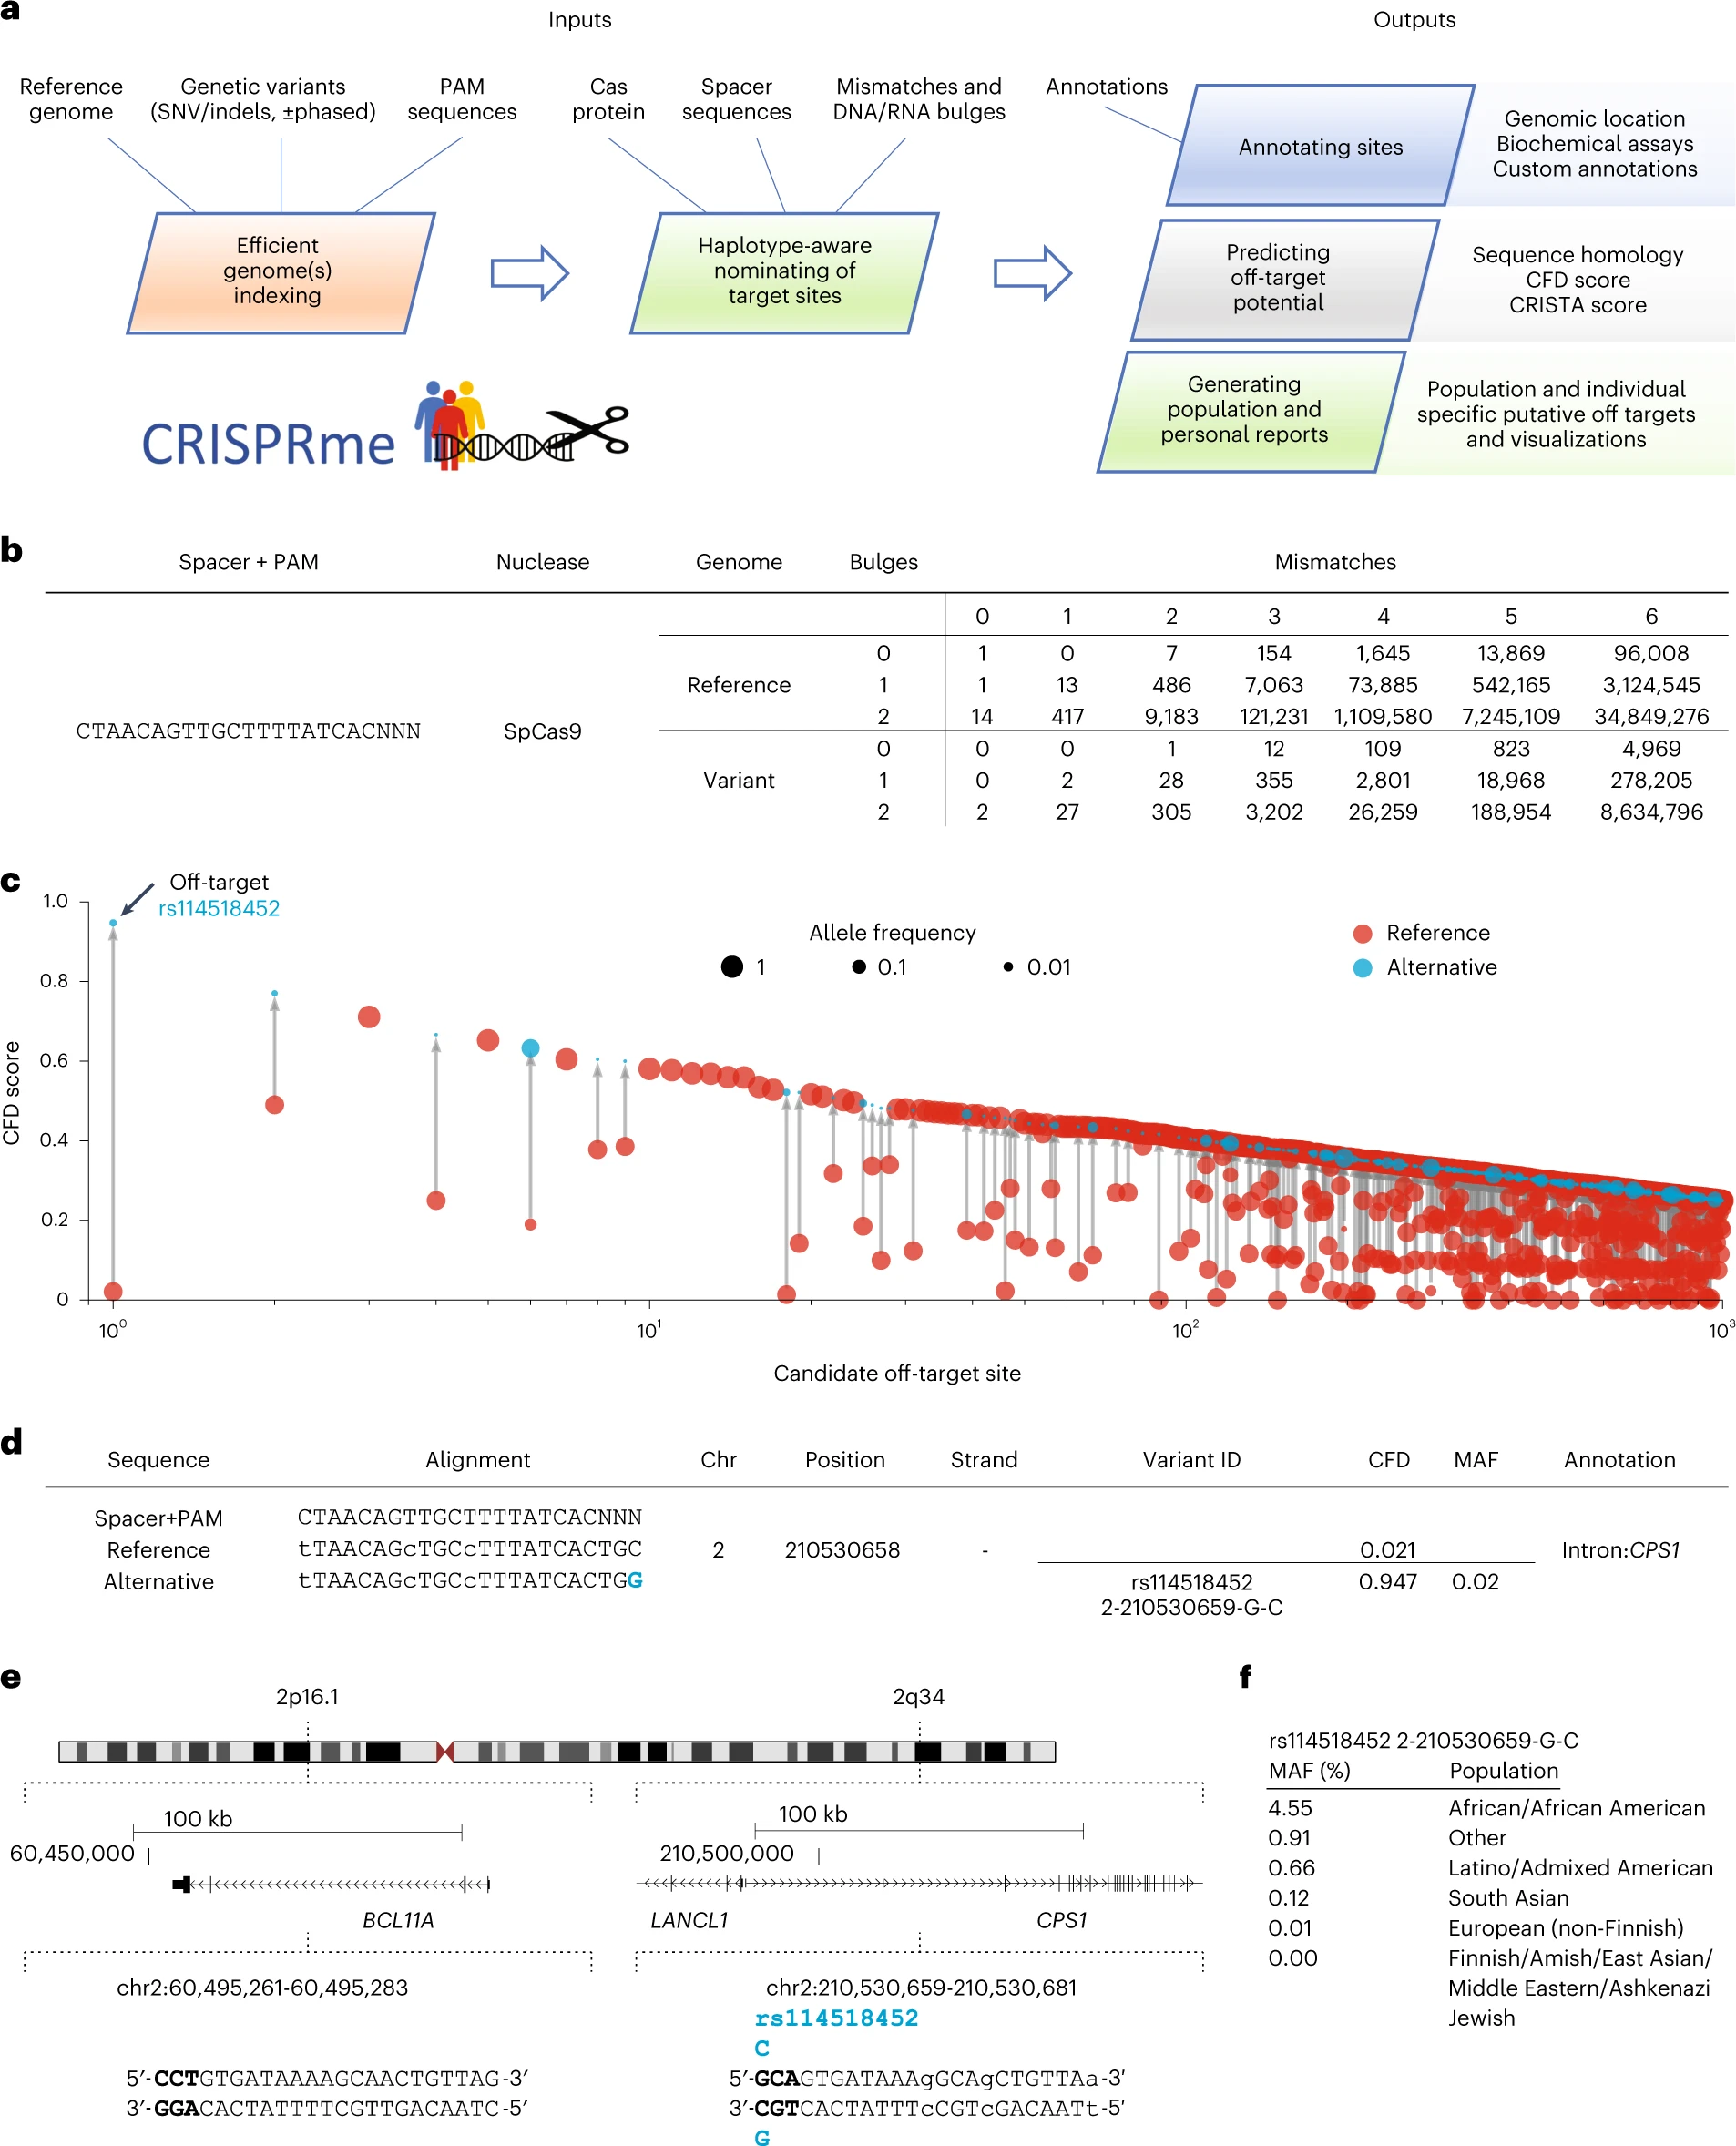
\includegraphics[width=\textwidth]{figures/crisprme1.png}
	\caption[CRISPRme provides web-based analysis of CRISPR-Cas gene editing off-target potential reflecting population genetic diversity]{\textbf{CRISPRme provides web-based analysis of CRISPR-Cas gene editing off-target potential reflecting population genetic diversity. (A)} CRISPRme software takes as input a reference genome, genetic variants, PAM sequence, Cas protein type, spacer sequence, homology threshold and genomic annotations and provides comprehensive, target-focused and individual-focused analyses of off-target potential. It is available as an online webtool and can be deployed locally or used offline as command-line software. \textbf{(B)} Analysis of the BCL11A-1617 spacer targeting the +58 erythroid enhancer with SpCas9, \texttt{NNN} PAM, 1000G variants, up to 6 mismatches and up to 2 bulges. \textbf{(C)} Top 1000 predicted off-target sites ranked by CFD score, indicating the CFD score of the reference and alternative allele if applicable, with allele frequency indicated by circle size. \textbf{(D)} The off-target site with the highest CFD score is created by the minor allele of rs114518452. Coordinates are for hg38 and 0-start for the potential off-target and 1-start for the variant-ID. MAF is based on 1000G. \textbf{(E)} The top predicted off-target site from CRISPRme is an allele-specific off-target with 3 mismatches to the BCL11A-1617 spacer sequence, where the rs114518452-C minor allele produces a de novo NGG PAM sequence. PAM sequence shown in bold and mismatches to BCL11A-1617 shown as lowercase. Coordinates are for hg38 and 1-start. \textbf{(F)} rs114518452 allele frequencies based on gnomAD v3.1. Coordinates are for hg38 and 1-start. Spacer shown as DNA sequence for ease of visual alignment.}
	\label{fig:crisprme1}
\end{figure} 
\crisprme is a web-based tool to predict off-target potential of CRISPR gene editing that accounts for genetic variation. It is available online at \url{http://crisprme.di.univr.it}. \crisprme can also be deployed to local, protected and isolated environments as a web app or command line utility, neither of which transfer or store data online, therefore respecting genomic privacy and regulations. \crisprme takes as input a Cas protein, gRNA spacer sequence and PAM, genome build, sets of variants (VCF files for populations or individuals), user-defined thresholds of mismatches and bulges and optional user-defined genomic annotations to produce comprehensive and personalized reports (\textbf{Fig.\ref{fig:crisprme1}(A)}). We have designed \crisprme to be flexible with support for new gene editors with variable and extremely relaxed PAM requirements \citep{walton2020unconstrained}. Thanks to a PAM encoding based on Aho-Corasick automata and an index based on a ternary search tree, CRISPRme can perform genome-wide exhaustive searches efficiently even with an NNN PAM, extensive mismatches (tested with up to seven) and RNA:DNA bulges (tested with up to two). Notably, a comprehensive search performed with up to six mismatches, two DNA/RNA bulges and a fully nonrestrictive PAM (NNN) on a small computational cluster node using 20 CPUs and 128 GB RAM (Intel Xeon CPU E5-2609 v4 clocked at 2.2 GHz) takes $\sim$34 h of real time and $\sim$152 h of CPU time (including both user and system times). All the 1000 G variants, including both single-nucleotide variants and indels, can be included in the search together with all the available metadata for each individual (sex, superpopulation and age), and the search operation takes into account observed haplotypes. Importantly, off-target sites that represent alternative alignments to a given genomic region are merged to avoid inflating the number of reported sites. Although several tools exist to enumerate off-targets, to our knowledge, only two command line tools \citep{lessard2017human, fennell2021calitas} incorporate genetic variants in the search. However, they have several limitations in terms of scalability to large searches, number of mismatches, bulges, haplotypes and variant file formats supported and do not provide an easy-to-use GUI. \crisprme generates several reports. (i) it summarizes for each gRNA all the potential off-targets found in the reference or variant genomes based on their mismatches and bulges (\textbf{Fig.\ref{fig:crisprme1}(B)}) and generates a file with detailed information on each of these candidate off-targets. 
(ii) it compares gRNAs to customizable annotations. By default, it classifies possible off-target sites based on GENCODE \citep{frankish2019gencode} (genomic features) and ENCODE \citep{encode2012integrated} (candidate cis-regulatory elements (cCREs)) annotations. It can also incorporate user-defined annotations in BED format, such as empiric off-target scores or cell-type-specific chromatin features (\textbf{Fig.\ref{fig:crisprme2}}).  
\begin{figure}
	\centering
	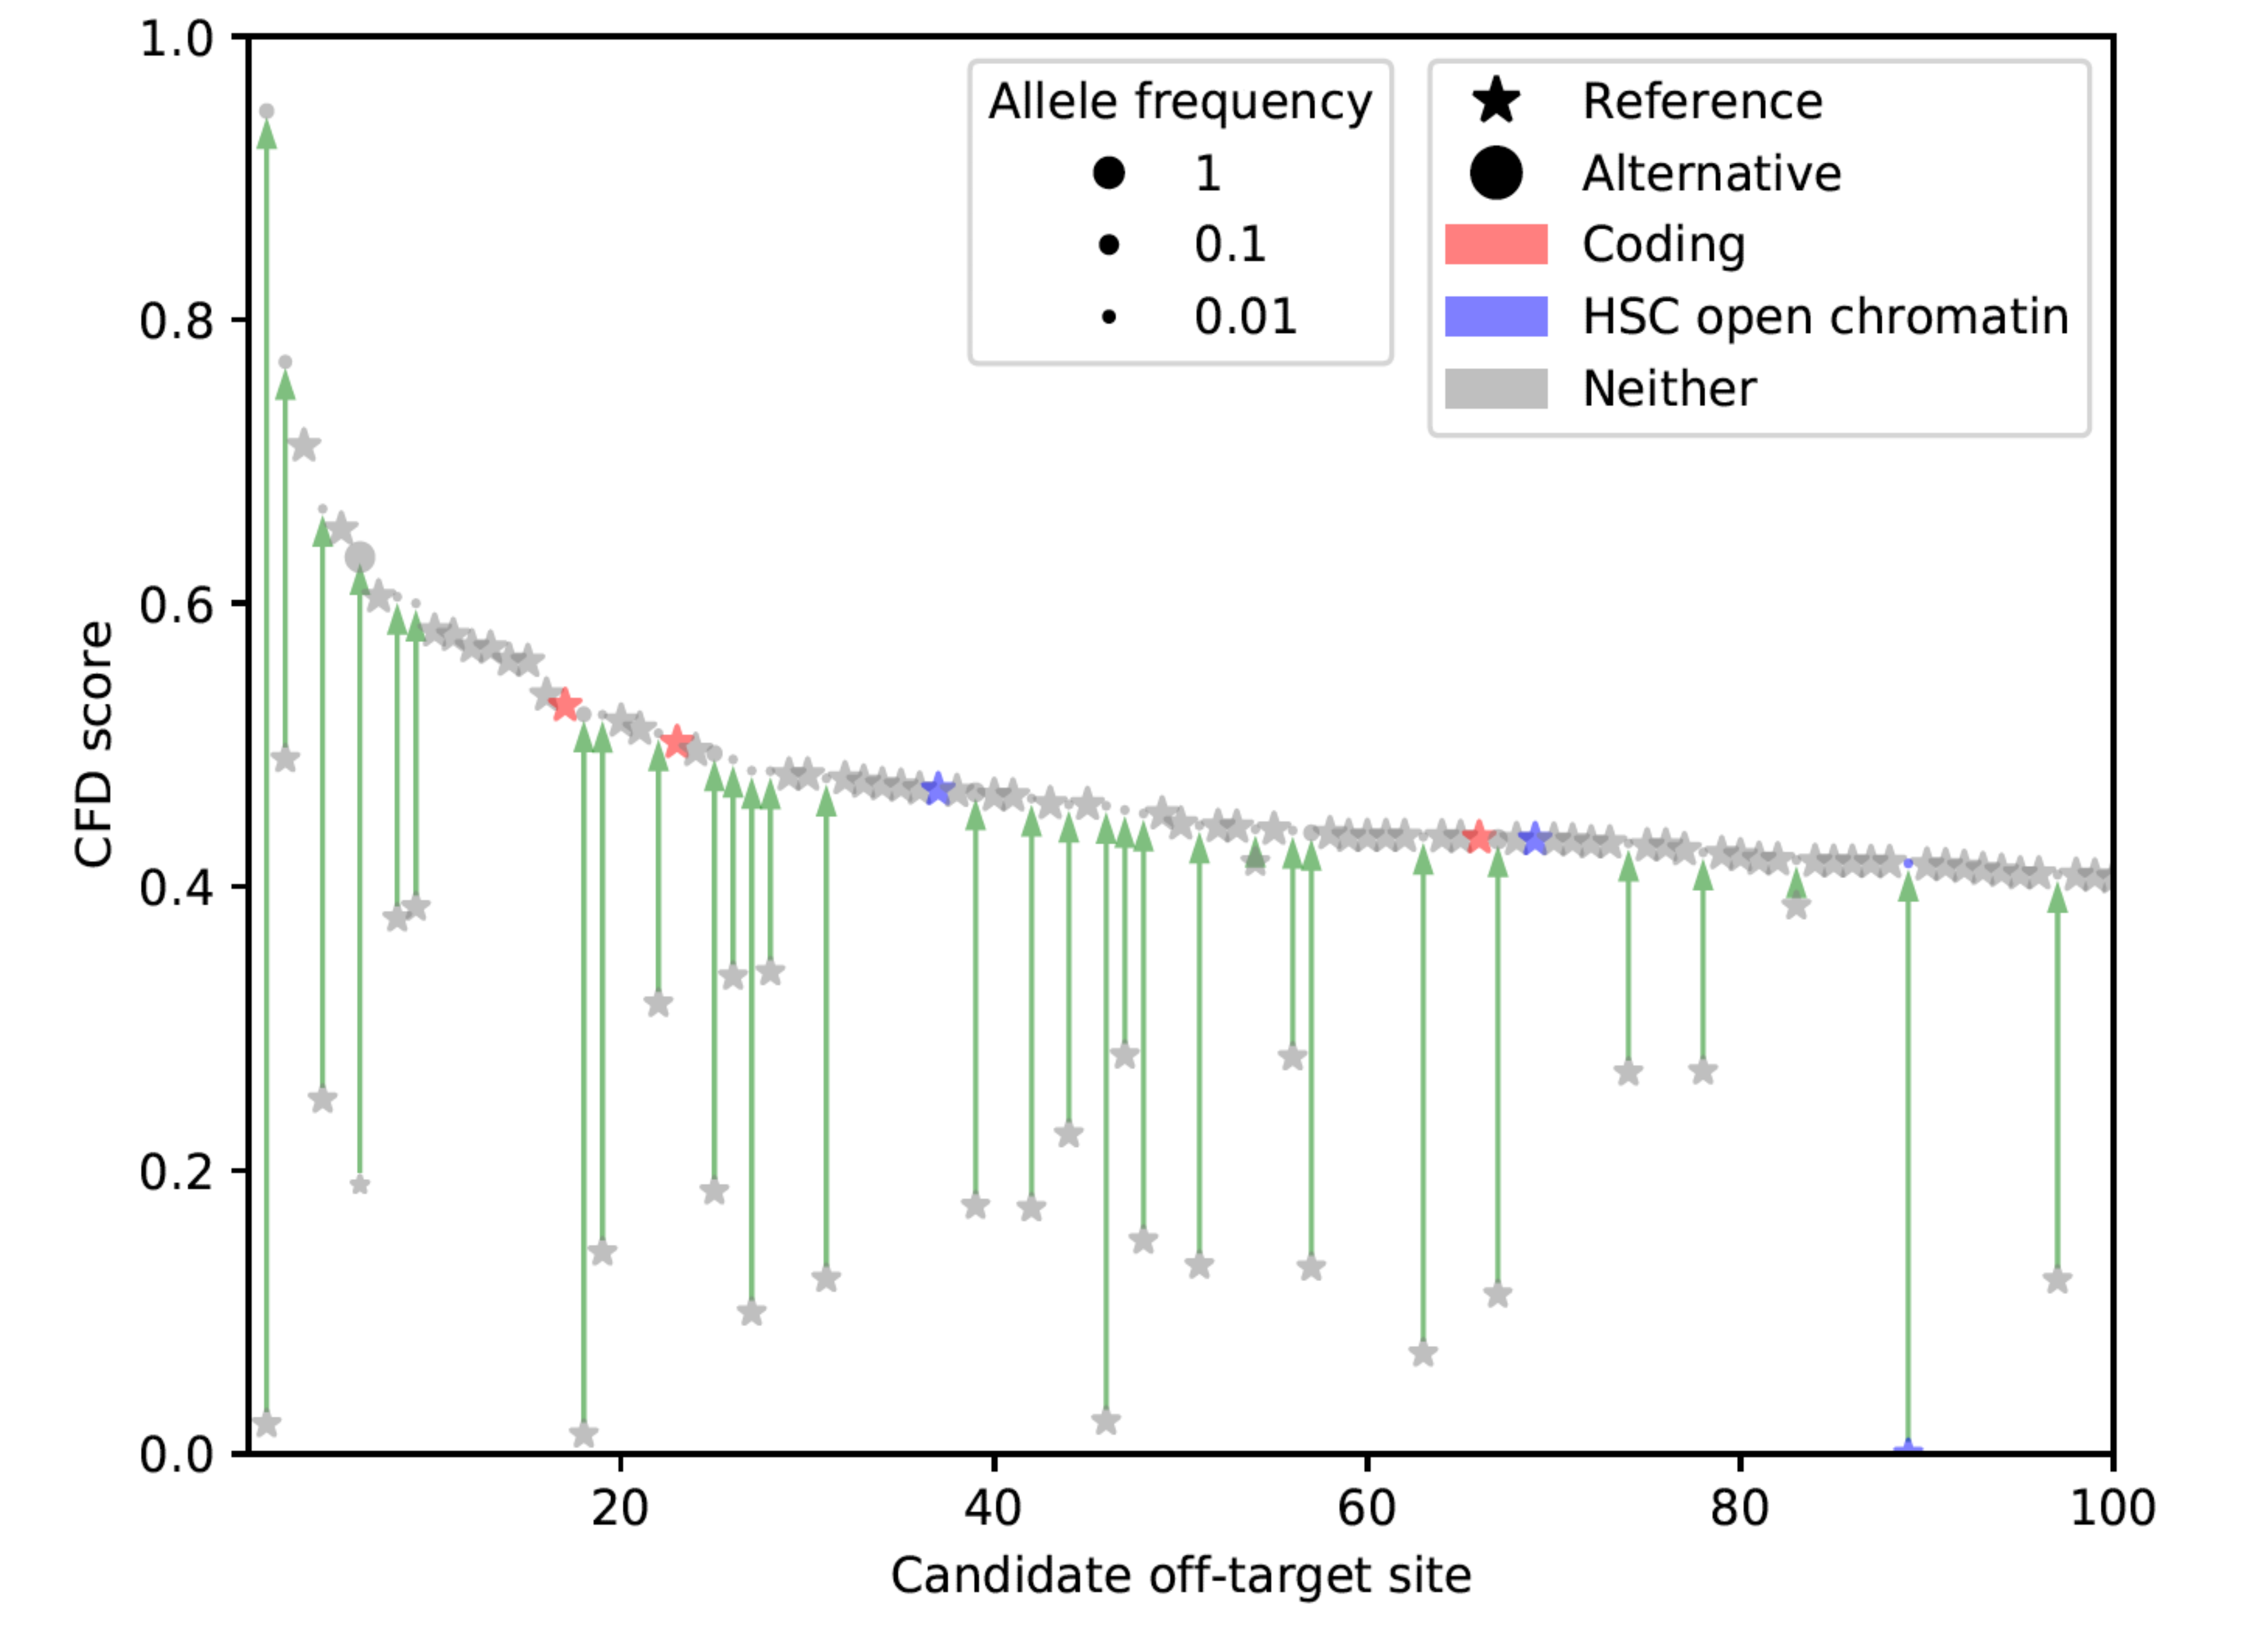
\includegraphics[width=\textwidth]{figures/crisprme2.png}
	\caption[Top 100 predicted off-target sites for BCL11A-1617 spacer by CFD score]{\textbf{Top 100 predicted off-target sites for BCL11A-1617 spacer by CFD score.} \crisprme search as in \textbf{Fig.\ref{fig:crisprme1}}. Candidate off-target sites within coding regions based on GENCODE annotations and ATAC-seq peaks in HSCs based on user-provided annotations (data from \citep{corces2016lineage}) are highlighted.}
	\label{fig:crisprme2}
\end{figure}
(iii) using 1000 G and/or HGDP variants, \crisprme reports the cumulative distribution of homologous sites based on the reference genome or superpopulation. These global reports could be used to compare a set of gRNAs based on how genetic variation impacts their predicted on- and off-target cleavage potential using cutting frequency determination (CFD) or CRISPR Target Assessment (CRISTA) scores \citep{abadi2017machine} (\textbf{Fig.\ref{fig:crisprme3}}). CRISPRme includes multiple scoring metrics and can be easily extended with new ones, including scores tailored for different editors. Finally, CRISPRme can generate personal genome focused reports called personal risk cards. These reports highlight private off-target sites due to unique genetic variants.
\begin{figure}
	\centering
	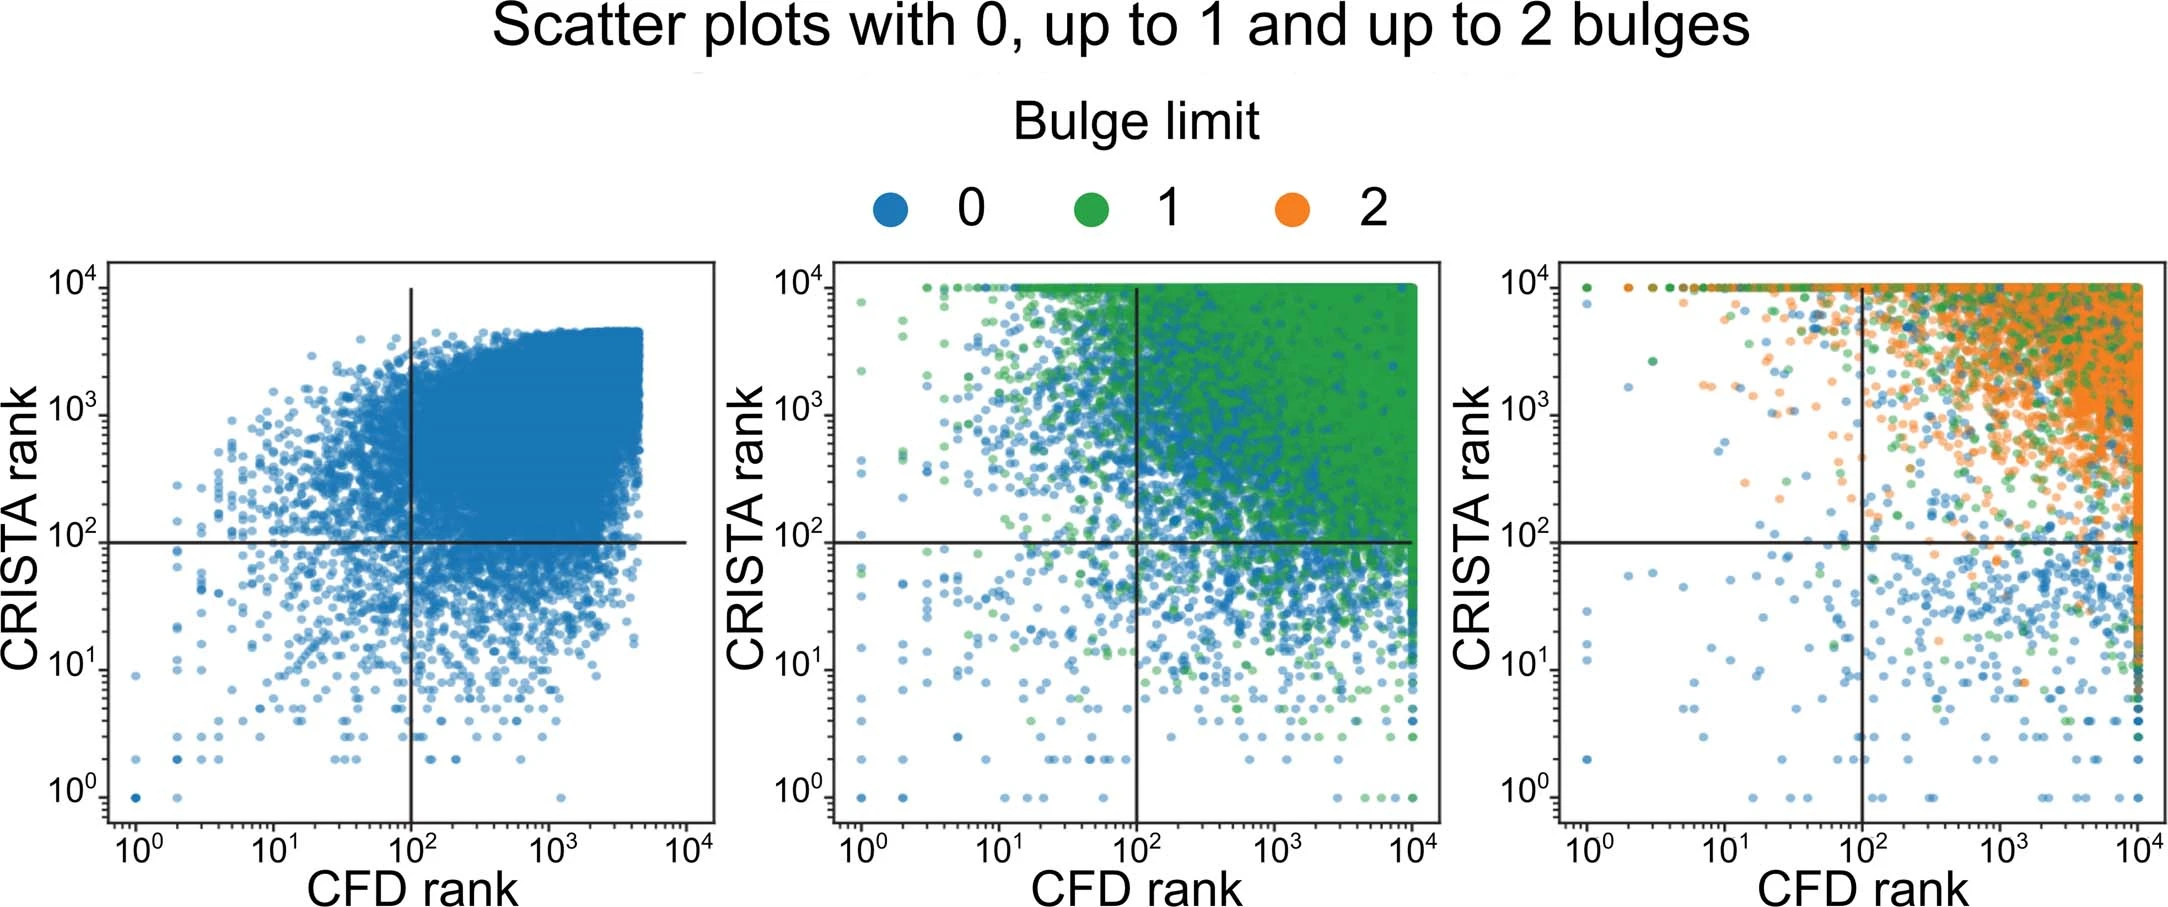
\includegraphics[width=\textwidth]{figures/crisprme3.png}
	\caption[Plots with rank ordered correlation between CFD and CRISTA reported targets]{\textbf{Plots with rank ordered correlation between CFD and CRISTA reported targets.} Scatter plots show from left to right, the correlation of ranked targets, extracted by selecting top 10,000 targets sorted by CFD and CRISTA score, respectively. The left plot shows the rank correlation of targets with 0 bulges (Pearson's correlation: 0.57, $p < 1e^{-10}$, Spearman's correlation: 0.55, $p < 1e^{-10}$), the center plot shows the rank correlation of targets with 1 bulge (Pearson's correlation: -0.16, $p < 1e^{-10}$, Spearman's correlation: -0.33, $p < 1e^{-10}$) and the right plot shows the rank correlation of targets with 2 bulges (Pearson's correlation: -0.55, $p < 1e^{-10}$, Spearman's correlation: -0.80, $p < 1e^{-10}$). The correlation values and $p$-values (two-sided) were calculated using standard functions from the Python scipy library. The colors represent the lowest count of bulges for each target, because the two scoring methods may prioritize different alignments and thus different number of mismatches and bulges pf the same target.}
	\label{fig:crisprme3}
\end{figure}
% -- A common allele-specific off-target for a gRNA in the clinic
\subsection{A common allele-specific off-target for a gRNA in the clinic}
\begin{figure}
	\centering
	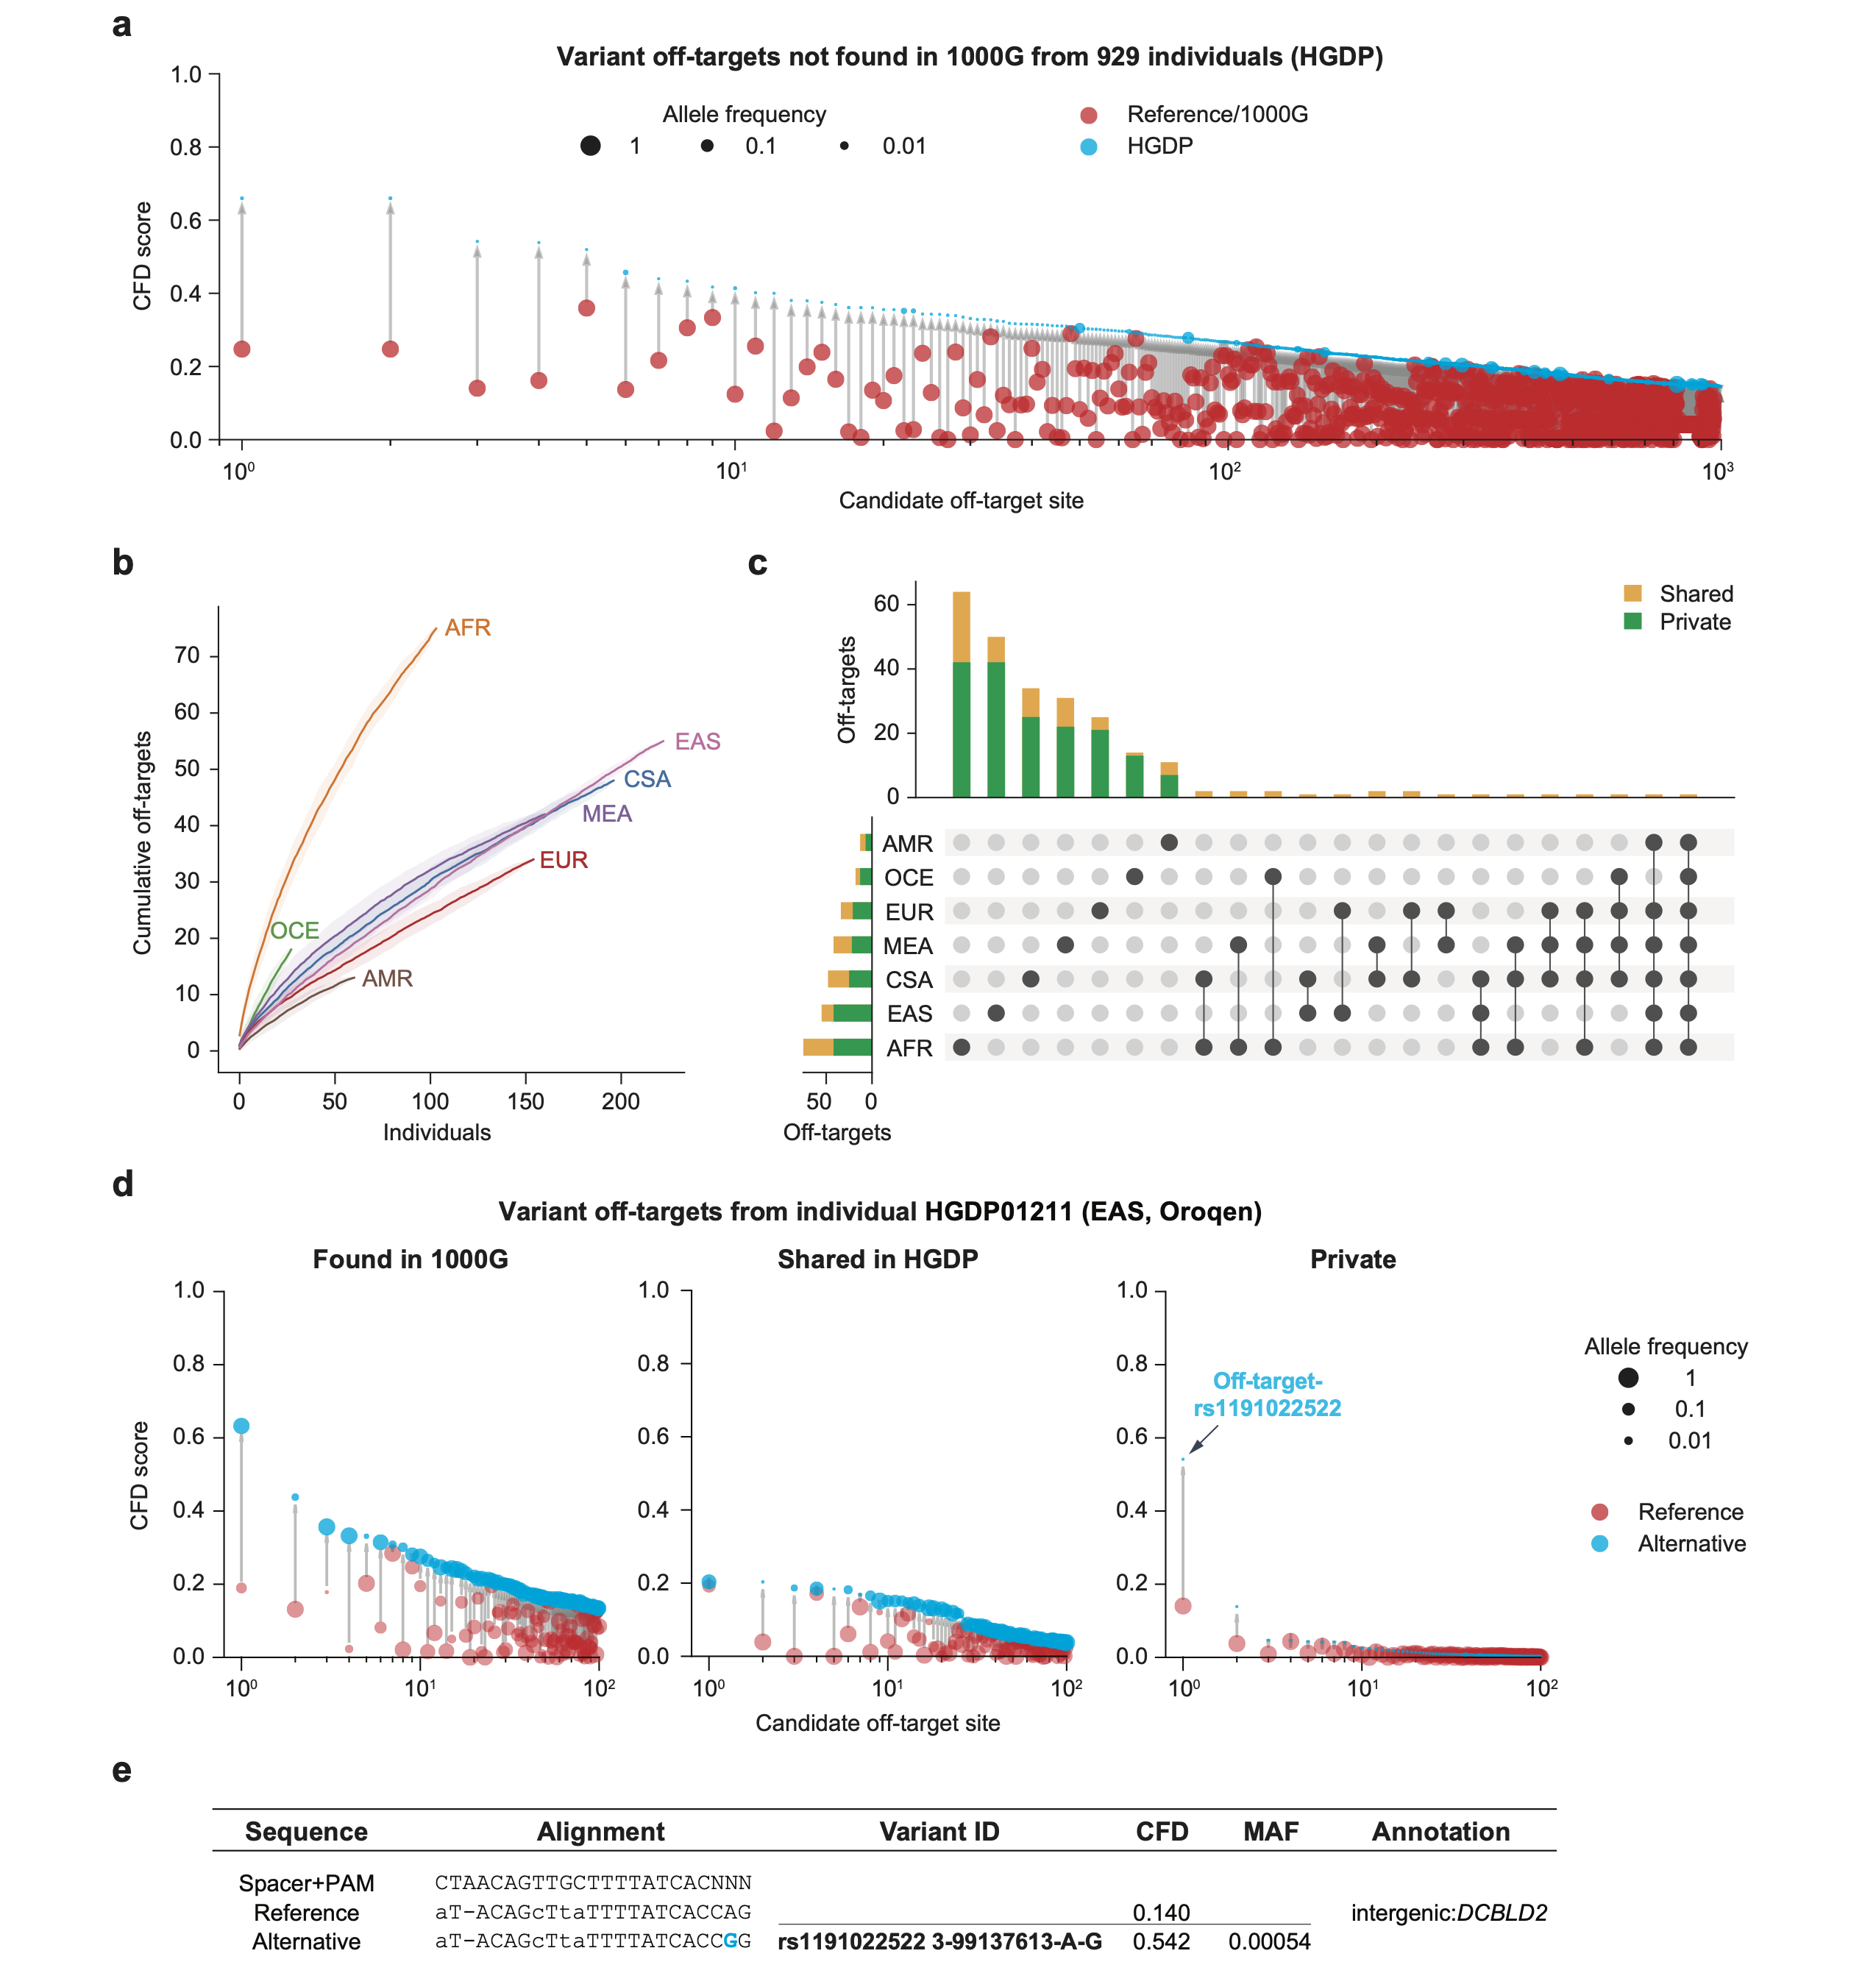
\includegraphics[width=\textwidth]{figures/crisprme4.png}
	\caption[\crisprme provides analysis of off-target potential of CRISPR-Cas gene editing reflecting population and private genetic diversity]{\textbf{\crisprme provides analysis of off-target potential of CRISPR-Cas gene editing reflecting population and private genetic diversity. (A)} \crisprme analysis was conducted with variants from HGDP comprising whole-genome sequencing of 929 individuals from 54 diverse human populations. HGDP variant off-targets with greater CFD scores than the reference genome or 1000 G were plotted and sorted by CFD score, with HGDP variant off-targets shown in blue and reference or 1000 G variant off-targets shown in red. \textbf{(B)} Cumulative distribution plot of HGDP variant off-targets with CFD $\geq 0.2$ and increase in CFD of $\geq 0.1$ per superpopulation (AFR: Africa, AMR: Americas, CSA: Central \& South Asia, EAS: East Asia, EUR: Europe, MEA: Middle East, OCE: Oceania). Individual samples from each of the seven superpopulations were shuffled 100 times to calculate the mean and 95\% confidence interval (shading around lines).  \textbf{(C)} Intersection analysis of HGDP variant off-targets with CFD $\geq 0.2$ and increase in CFD of $\geq 0.1$. Shared variants (black) were found in two or more HGDP samples whereas private variants (gray) were limited to a single sample. \textbf{(D)} \crisprme analysis of a single individual (HGDP01211) showing the top 100 variant off-targets from each of the following three categories: shared with 1000G variant off-targets (left panel), higher CFD score compared to reference genome and 1000 G but shared with other HGDP individuals (center panel) and higher CFD score compared to reference genome and 1000 G with variant not found in other HGDP individuals (right panel). For the center and right panels, reference refers to CFD score from reference genome or 1000 G variants.  \textbf{(E)} The top predicted private off-target site from HGDP01211 is an allele-specific off-target where the rs1191022522-G minor allele produces a canonical NGG PAM sequence in place of a noncanonical NAG PAM sequence. Spacer shown as DNA sequence for ease of visual alignment.}
	\label{fig:crisprme4}
\end{figure}
We tested \crisprme with a gRNA (\#1617) targeting a GATA1 binding motif at the +58 erythroid enhancer of BCL11A \citep{canver2015bcl11a, wu2019highly}. A recent clinical report described two patients, one with SCD and one with $\beta$-thalassemia, each treated with autologous gene modified HSPCs edited with Cas9 and this gRNA, who showed sustained increases in fetal hemoglobin, transfusion independence and absence of vaso-occlusive episodes (in the patient with SCD) following therapy. This study, as well as prior preclinical studies with the same gRNA (\#1617), did not reveal evidence of off-target editing in treated cells when considering off-target sites nominated by bioinformatic analysis of the human reference genome and empiric analysis of in vitro genomic cleavage potential \citep{frangoul2021crispr, wu2019highly, demirci2019durable}.  \crisprme analysis found that the predicted off-target site with both the greatest CFD score and the greatest increase in CFD score from the reference to alternative allele was at an intronic sequence of CPS1 (\textbf{Fig.\ref{fig:crisprme1}(C)} and \textbf{(D)}),  a genomic target subject to common genetic variation (modified by a SNP with MAF $\geq$ 1\%). CFD scores range from 0 to 1, where the on-target site has a score of 1. The alternative allele rs114518452-C generates a TGG PAM sequence (that is, the optimal PAM for SpCas9) for a potential off-target site with three mismatches and a CFD score (CFD$_{alt}$ 0.95) approaching that of the on-target site (\textbf{Fig.\ref{fig:crisprme1}(E)}). In contrast, the reference allele rs114518452-G disrupts the PAM to TGC, which markedly reduces predicted cleavage potential (CFD$_{ref}$ 0.02). rs114518452-C has an overall MAF of 1.33\% in gnomAD v3.1, with an MAF of 4.55\% in African/African American, 0.91\% in Other, 0.66\% in Latino/Admixed American, 0.12\% in South Asian, 0.01\% in European (non-Finnish) and 0.00\% in all other populations represented in gnomAD (\textbf{Fig.\ref{fig:crisprme1}(F)}). To consider the off-target potential that could be introduced by personal genetic variation that would not be predicted by 1000 G variants, we analyzed HGDP variants identified from whole-genome sequences of 929 individuals from 54 diverse human populations. We observed 249 candidate off-targets for gRNA \#1617 with CFD $\geq 0.2$ for which the CFD score in HGDP exceeded that found for either the reference genome or 1000 G variants by at least 0.1 (\textbf{Fig.\ref{fig:crisprme4}(A)} and \textbf{Fig.\ref{fig:crisprme5}}). hese additional variant off-targets not found from 1000 G were observed in each superpopulation, with the greatest frequency in the African superpopulation (\textbf{Fig.\ref{fig:crisprme4}(B)}); 229 (92.0\%) of these variant off-targets were unique to a superpopulation, and 172 (69.1\%) of these were private to just one individual (\textbf{Fig.\ref{fig:crisprme4}(C)}). Furthermore, single-individual-focused searches (for example, an analysis of HGDP01211, an individual of the Oroqen population within the East Asian superpopulation) showed that most variant off-targets (with higher CFD score than reference) were due to variants also found in 1000 G (n = 32369, 90.4\%), a subset were due to variants shared with other individuals from HGDP but absent from 1000 G (n = 3177, 8.9\%) and a small fraction were private to the individual (n = 234, 0.7\%) (\textbf{Fig.\ref{fig:crisprme4}(D)}).  Among these private off-targets was one generated by a variant (rs1191022522, 3-99137613-A-G, gnomAD v3.1 MAF 0.0053\%) where the alternative allele produces a canonical NGG PAM that increases the CFD score from 0.14 to 0.54 (\textbf{Fig.\ref{fig:crisprme4}(D)} and \textbf{(E)}).
\begin{figure}
	\centering
	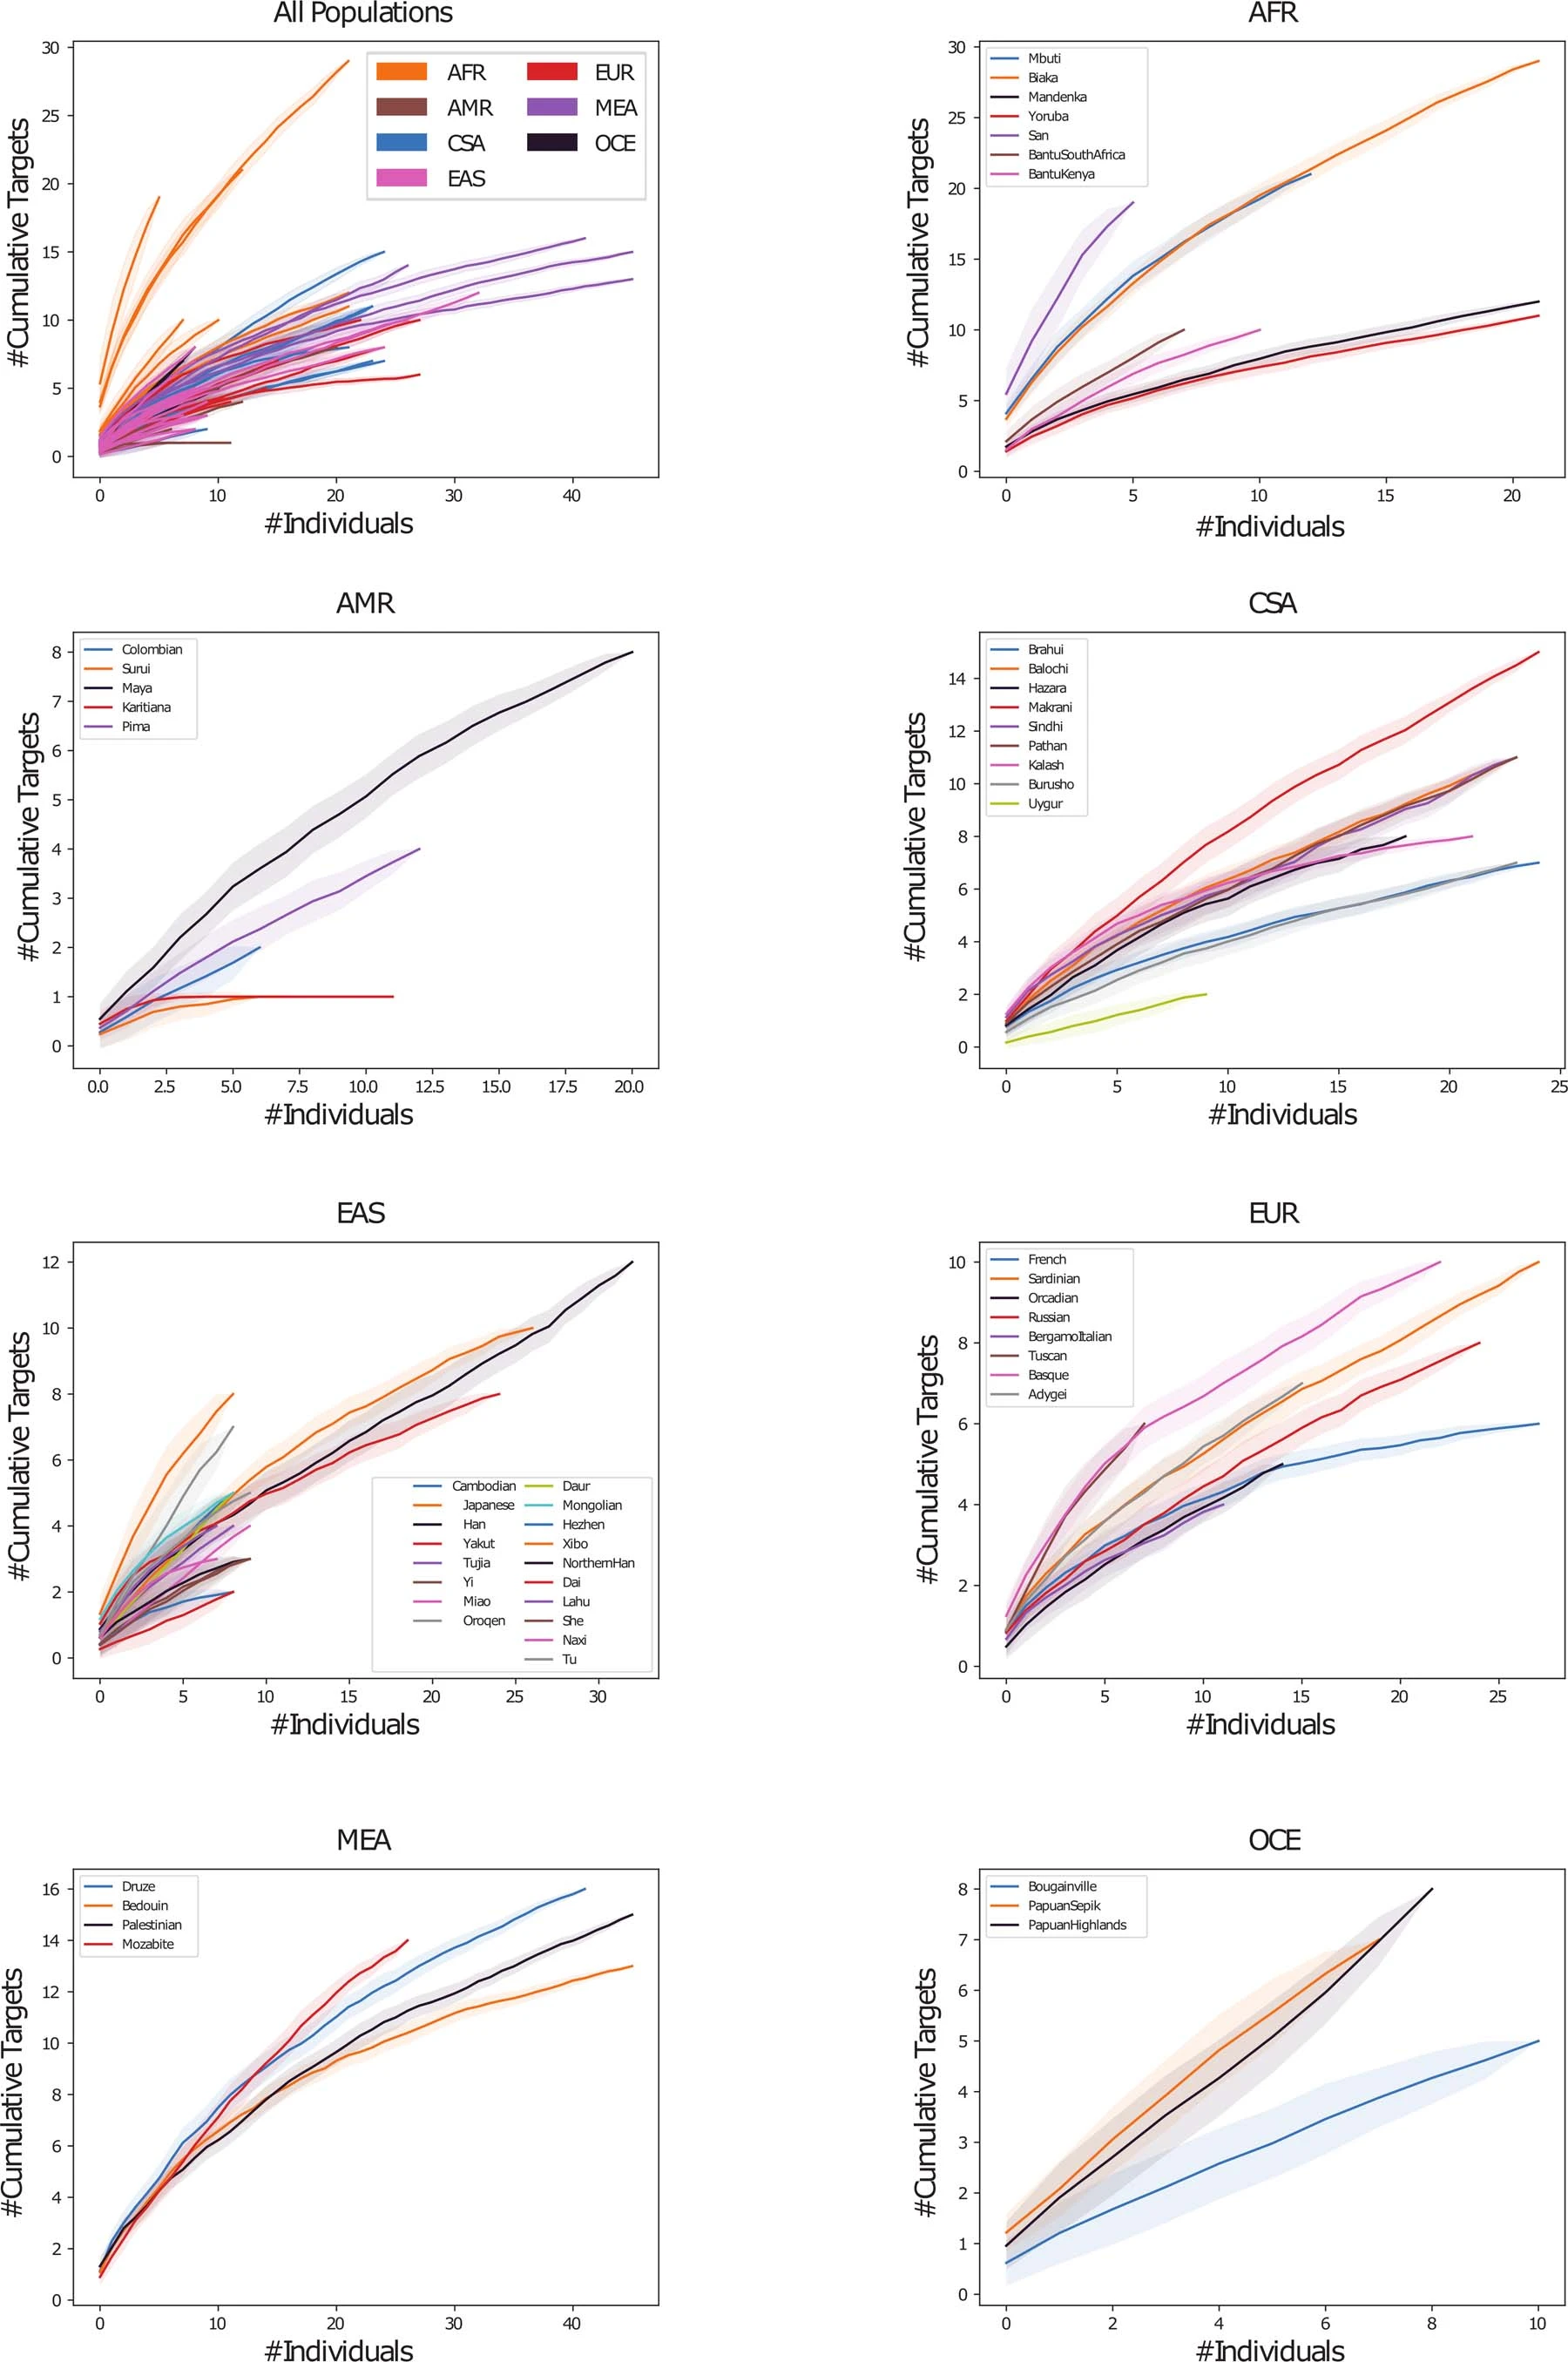
\includegraphics[width=\textwidth]{figures/crisprme5.png}
	\caption[HGDP superpopulation distribution plots]{\textbf{HGDP superpopulation distribution plots.} HGDP variant off-targets with CFD $\geq 0.2$ and increase in CFD of $\geq 0.1$.  Individual samples from each of the seven superpopulations were shuffled 100 times to calculate the mean and 95\% confidence interval. First panel shows distribution within all 54 discrete populations, colored by superpopulation. Additional seven panels show distribution of discrete populations within each listed superpopulation.}
	\label{fig:crisprme5}
\end{figure}
o experimentally test the top predicted off-target from CRISPRme, we identified a CD34+ HSPC donor of African ancestry heterozygous for rs114518452-C, the variant predicted to introduce the greatest increase in off-target cleavage potential (\textbf{Fig.\ref{fig:crisprme1}(C)-(F)}).  We performed ribonucleoprotein (RNP) electroporation using a gene editing protocol that preserves engrafting HSC function. Amplicon sequencing analysis showed 92.0 $\pm$ 0.5\% indels at the on-target site and 4.8 $\pm$ 0.5\% indels at the off-target site. For reads spanning the variant position, indels were strictly found at the alternative PAM-creation allele without indels observed at the reference allele (\textbf{Fig.\ref{fig:crisprme6}(A)-(C)}),  suggesting 9.6 $\pm$ 1.0\% off-target editing of the alternative allele. In an additional six HSPC donors homozygous for the reference allele rs114518452-G/G, 0.00 $\pm$ 0.00\% indels were observed at the off-target site, suggesting strict restriction of off-target editing to the alternative allele (\textbf{Fig.\ref{fig:crisprme6}(D)}).
\begin{figure}
	\centering
	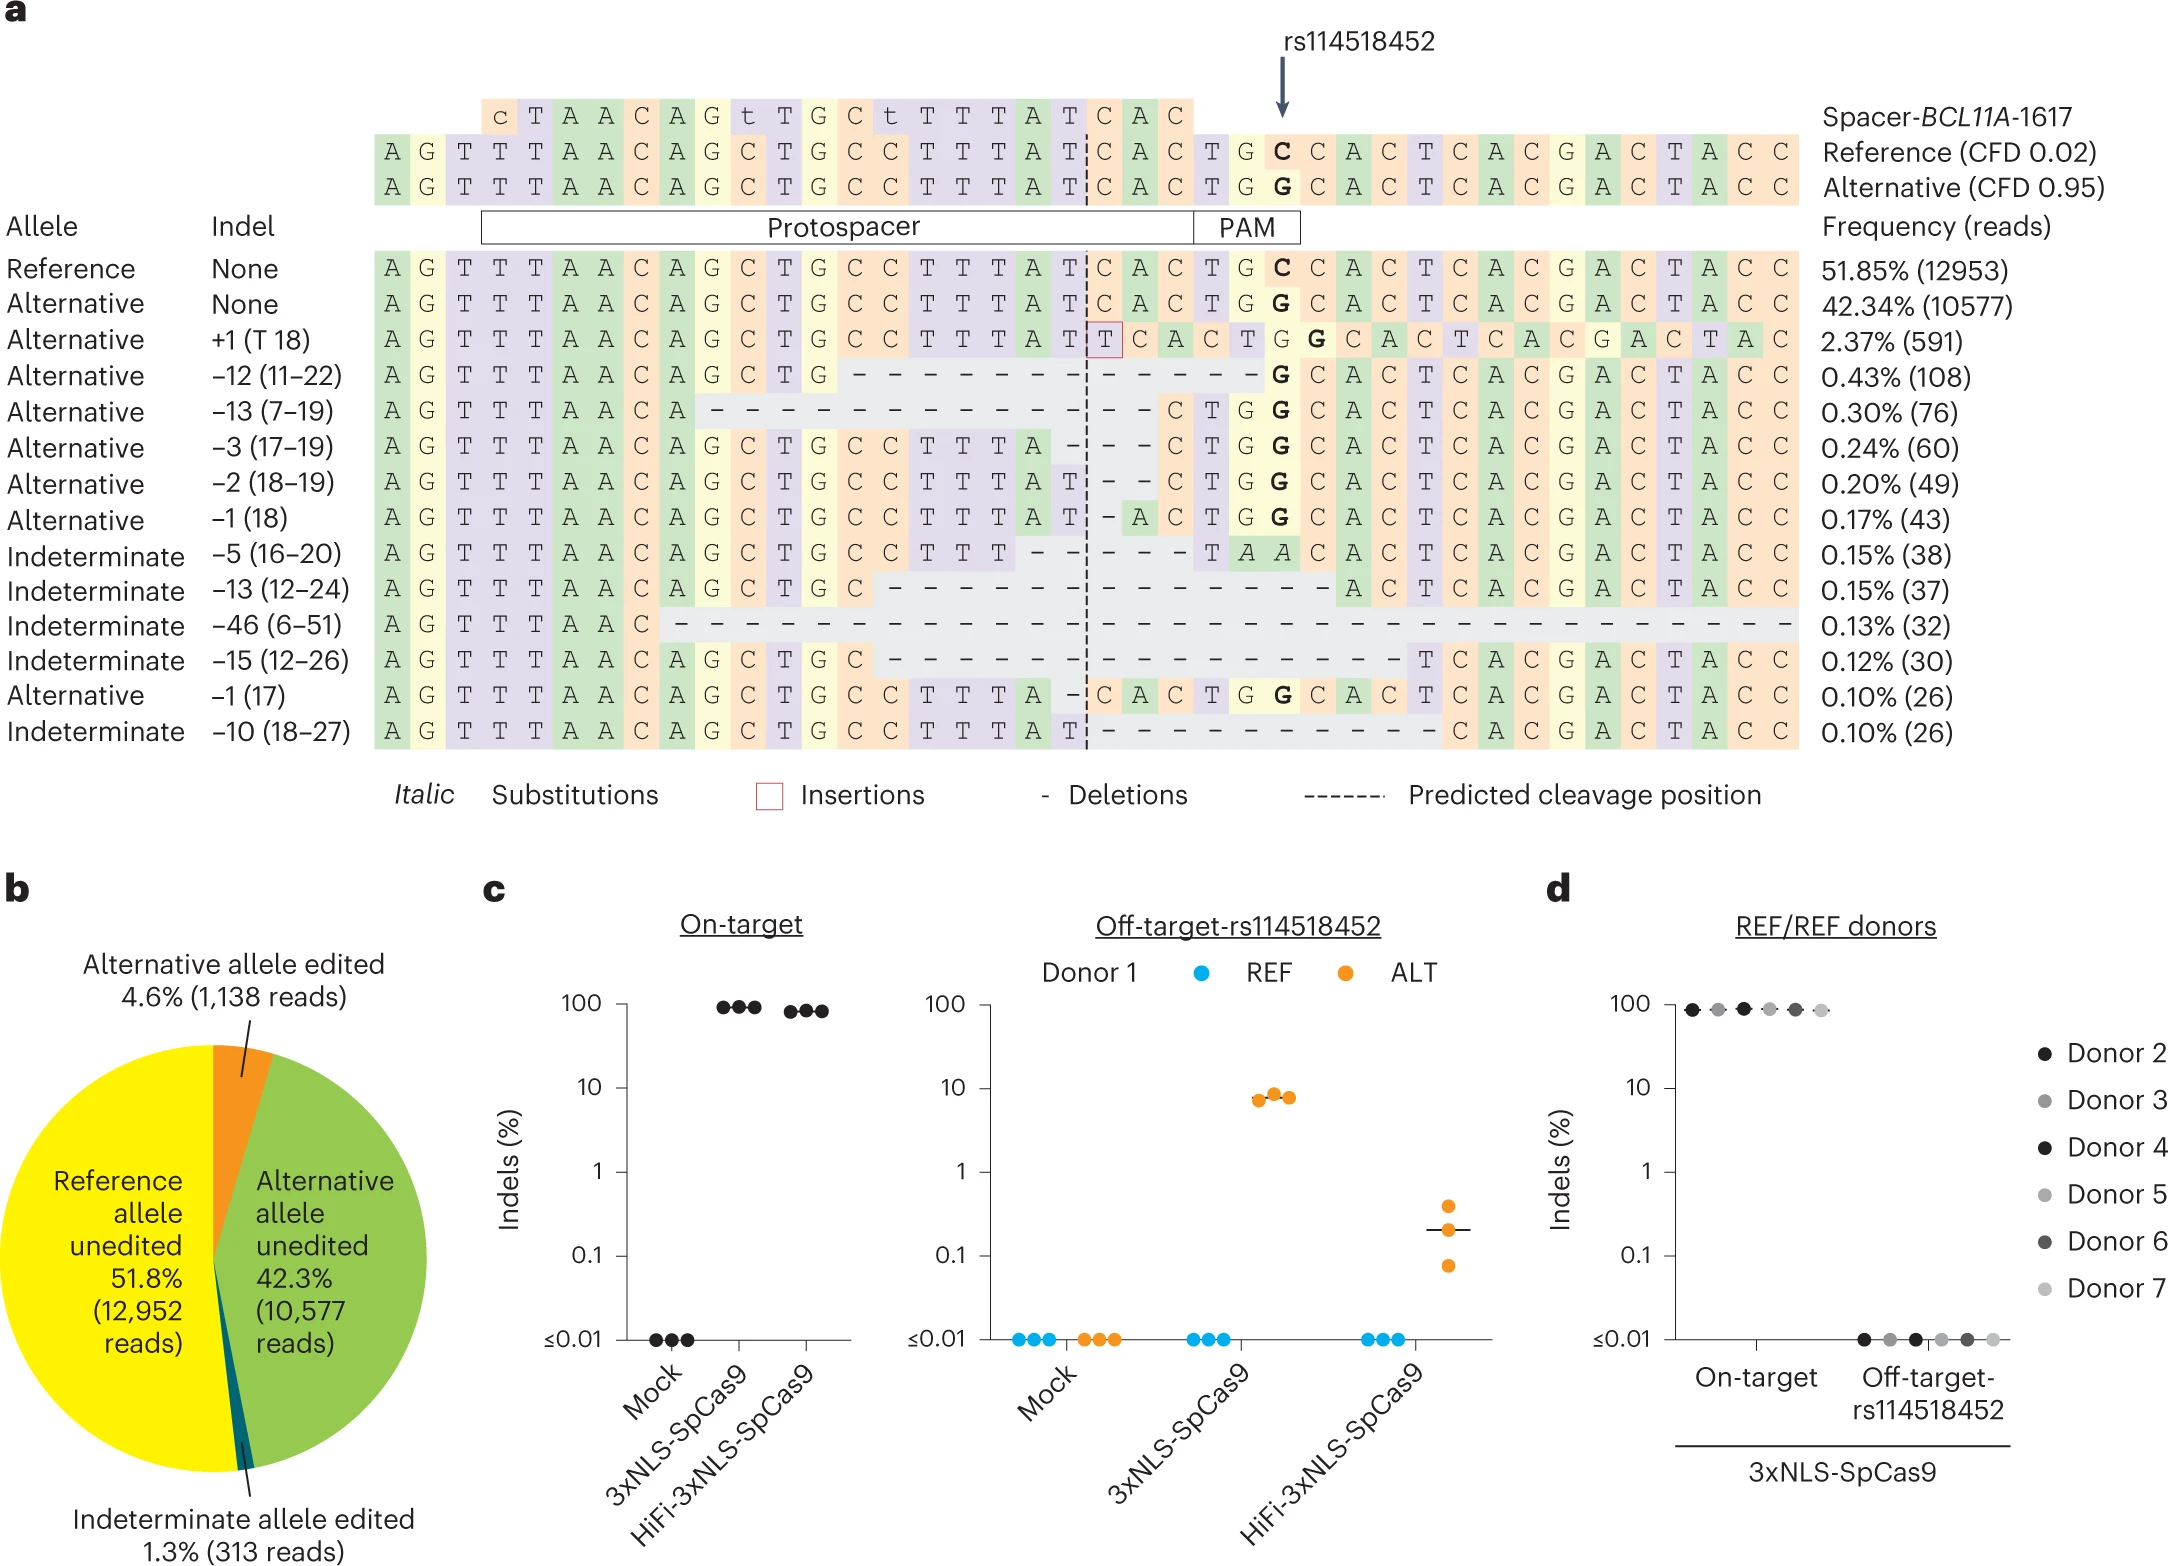
\includegraphics[width=\textwidth]{figures/crisprme6.png}
	\caption[Allele-specific off-target editing by a BCL11A enhancer targeting gRNA in clinical trials associated with a common variant in African-ancestry populations]{\textbf{Allele-specific off-target editing by a BCL11A enhancer targeting gRNA in clinical trials associated with a common variant in African-ancestry populations. (A)} Human CD34+ HSPCs from a donor heterozygous for rs114518452-G/C (donor 1, REF/ALT) were subject to 3xNLS-SpCas9:sg1617 RNP electroporation (NLS: nuclear localization signal) followed by amplicon sequencing of the off-target site around chr2:210,530,659-210,530,681 (off-target-rs114518452 in 1-start hg38 coordinates). CFD scores for the reference and alternative alleles are indicated, and representative aligned reads are shown. Spacer shown as DNA sequence for ease of visual alignment, with mismatches indicated by lowercase and the rs114518452 position shown in bold.  \textbf{(B)} Reads classified based on allele (indeterminate if the rs114518452 position is deleted) and presence or absence of indels (edits). \textbf{(C)} Huma CD34+ HSPCs ffrom a donor heterozygous for rs114518452-G/C (donor 1) were subject to 3xNLS-SpCas9:sg1617 RNP electroporation,  HiFi-3xNLS-SpCas9:sg1617 RNP electroporation, or no electroporation (mock) followed by amplicon sequencing of the on-target and off-target-rs114518452 sites. each dot represents an independentbiological replicate (n = 3), and lines represent medians. Indel frequency was quantified for reads aligning to either the reference (REF) or alternative (ALT) allele. \textbf{(D)} Human CD34+ HSPCs from six donors homozygous for rs114518452-G/G (donors 2–7, REF/REF) were subject to 3xNLS-SpCas9:sg1617 RNP electroporation with one biological replicate per donor followed by amplicon sequencing of the on-target and off-target-rs114518452 sites.}
	\label{fig:crisprme6}
\end{figure}
The on-target BCL11A intronic enhancer site is on chr2p, whereas the off-target-rs114518452 site is on chr2q within an intron of a noncanonical transcript of CPS1. Inversion PCR demonstrated inversion junctions consistent with the presence of $\sim$150 Mb pericentric inversions between BCL11A and the off-target site only in edited HSPCs carrying the alternative allele (\textbf{Fig.\ref{fig:crisprme7}(A)} and \textbf{(B)}). Deep sequencing of the inversion junction showed that inversions were restricted to the alternative allele in the heterozygous cells (\textbf{Fig.\ref{fig:crisprme7}(C)} and \textbf{(D)}). Droplet digital PCR revealed these inversions to be present at 0.16 $\pm$ 0.04\% allele frequency (\textbf{Fig.\ref{fig:crisprme7}(E)}). Various high-fidelity Cas9 variants may improve the specificity of gene editing, although at the possible cost of reduced efficiency \citep{schmid2020highly}. Gene editing following the same electroporation protocol using a HiFi variant 3xNLS-SpCas9 (R691A) \citep{vakulskas2018high} in heterozygous cells revealed 82.3 $\pm$ 1.6\% on-target indels with only 0.1 $\pm$ 0.1\% indels at the rs114518452-C off-target site (that is, a $\sim$48-fold reduction compared to SpCas9) (\textbf{Fig.\ref{fig:crisprme6}(C)}). Inversions were not detected following HiFi-3xNLS-SpCAs9 editing (\textbf{Fig.\ref{fig:crisprme7}(B)} and \textbf{(E)}).
\begin{figure}
	\centering
	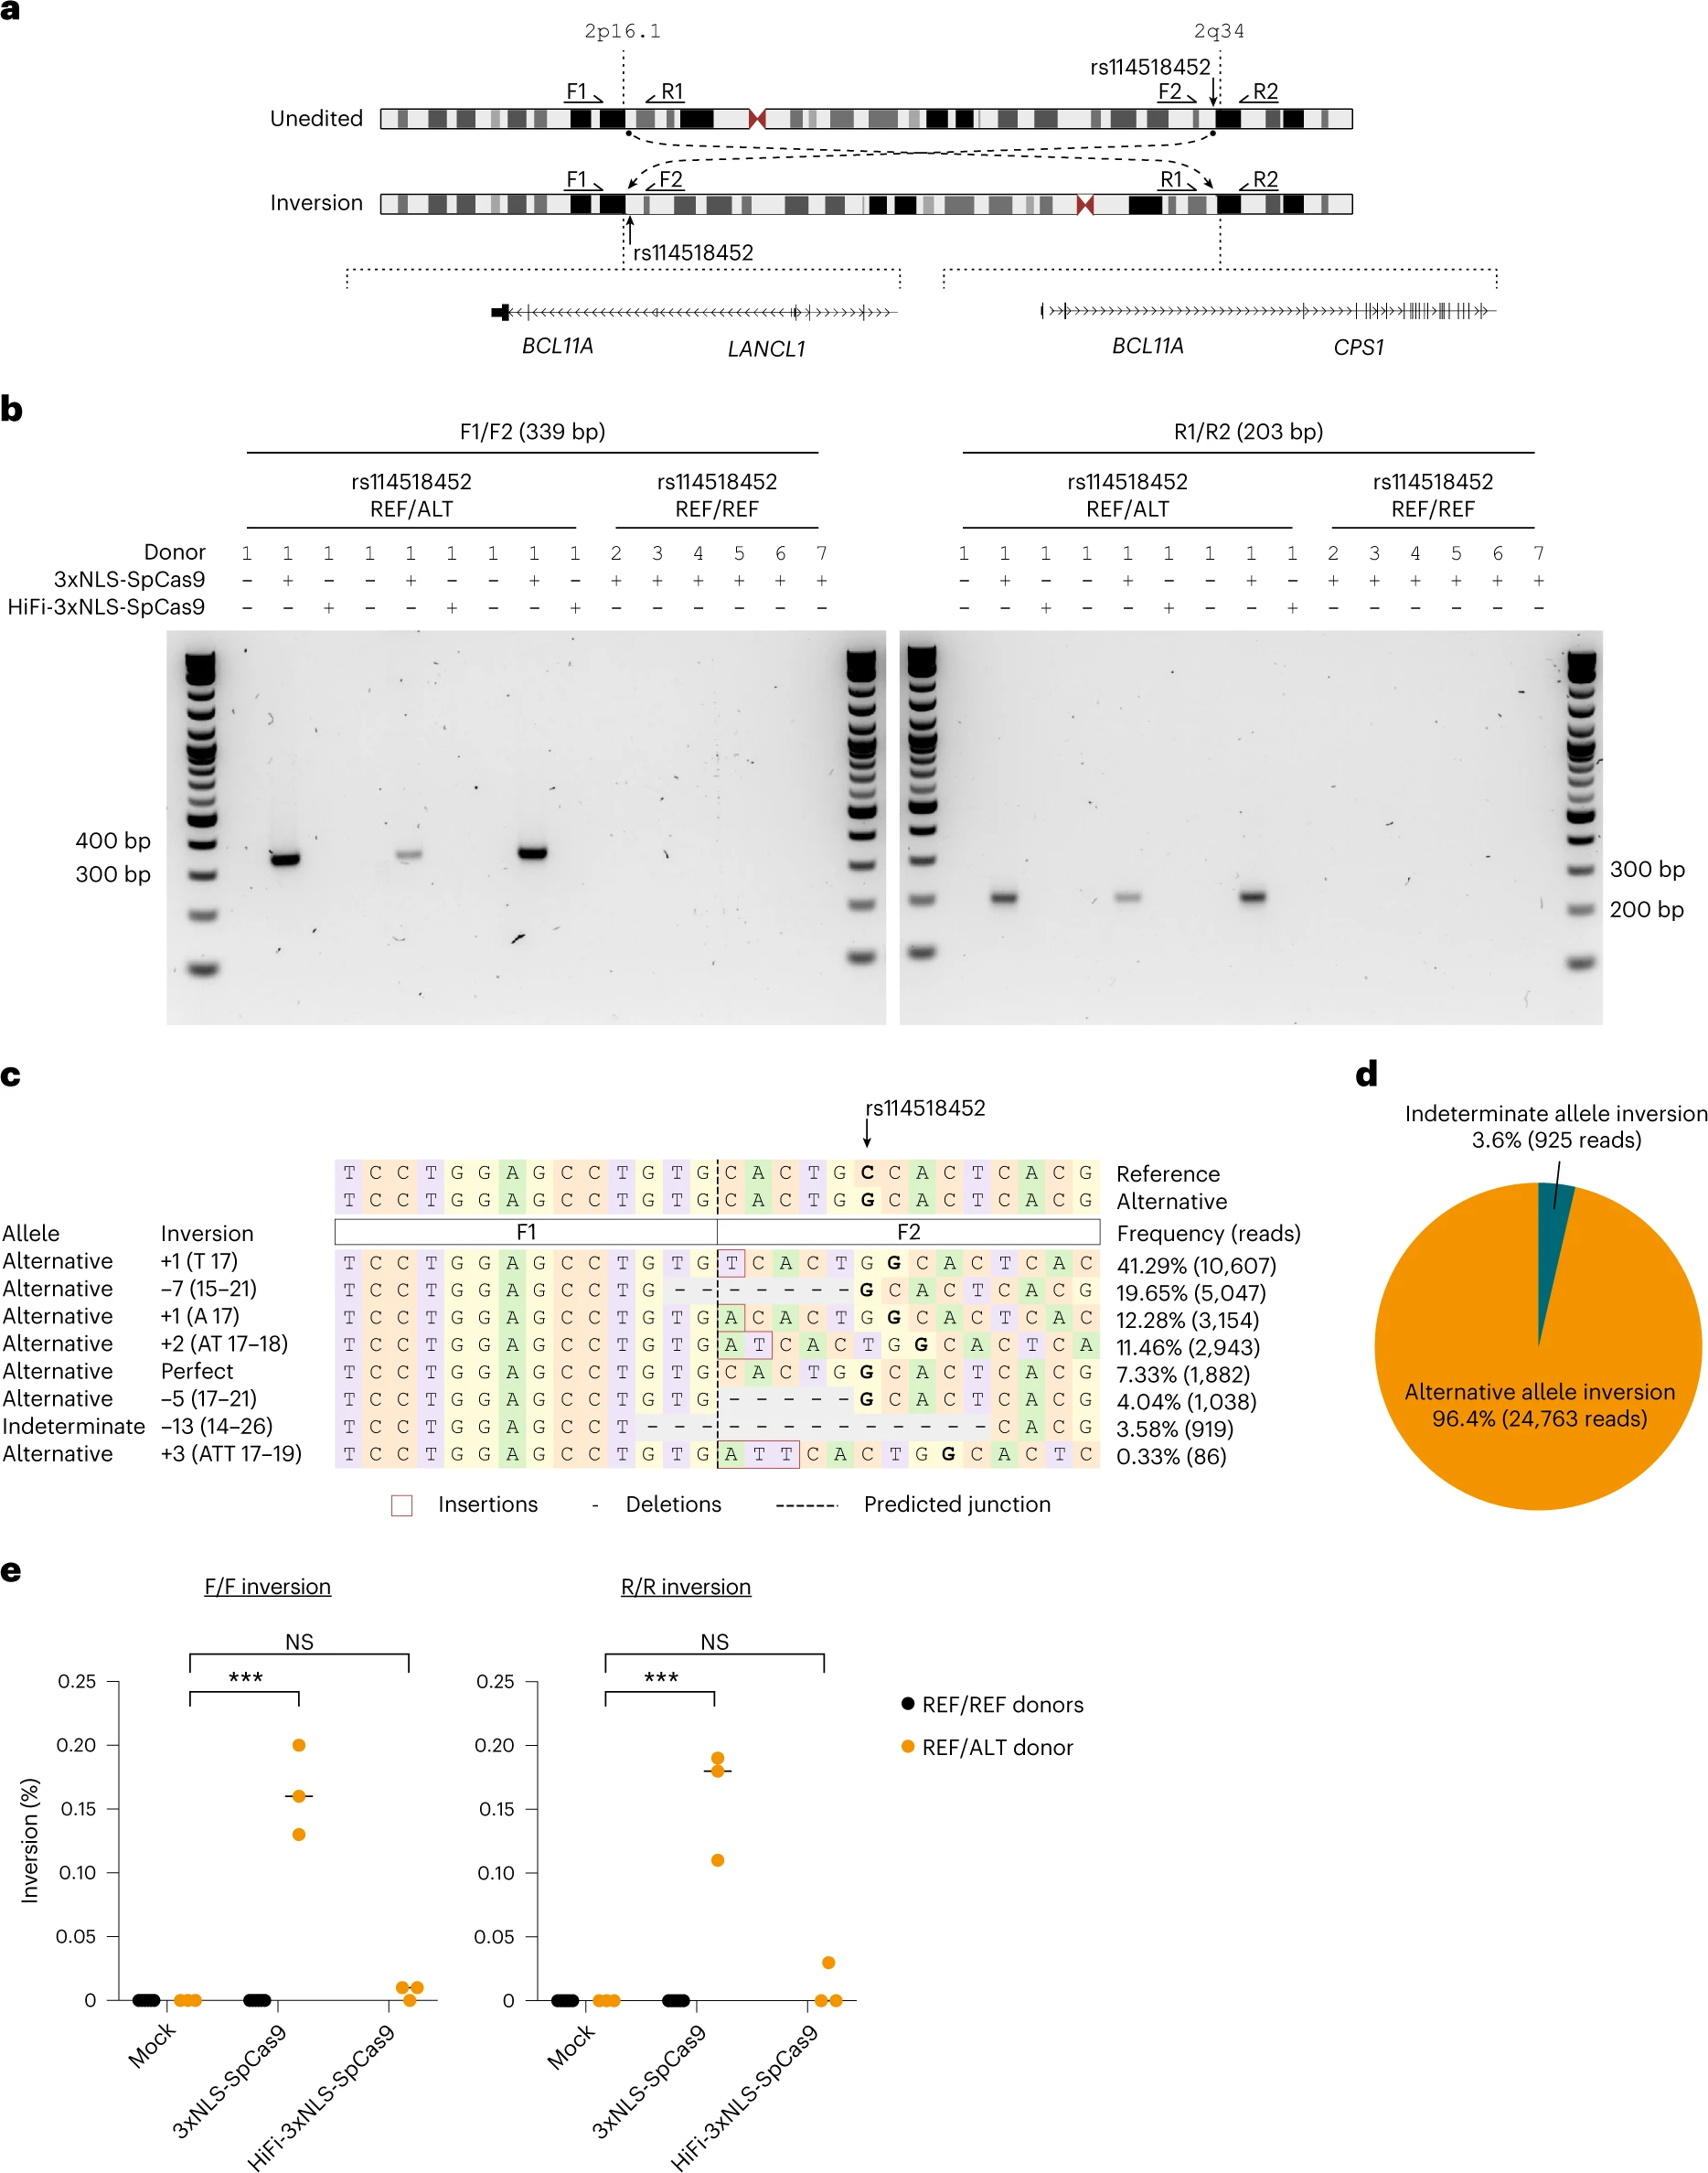
\includegraphics[width=\textwidth]{figures/crisprme7.png}
	\caption[Allele-specific pericentric inversion following BCL11A enhancer editing due to off-target cleavage]{\textbf{Allele-specific pericentric inversion following BCL11A enhancer editing due to off-target cleavage. (A)} Concurrent cleavage of the on-target and off-target-rs114518452 sites could lead to pericentric inversion of chr2 as depicted. PCR primers F1, R1, F2 and R2 were designed to detect potential inversions. \textbf{(B)} Human CD43+ HSPCs from a donor heterozygous for rs114518452-G/C (donor 1) were subject to 3xNLS-SpCas9:sg1617 RNP electroporation, HiFi-3xNLS-SpCas9:sg1617 RNP electroporation or no electroporation with three biological replicates. Human CD43+ HSPCs from six donors homozygous for rs114518452-G/G (donors 2–7, REF/REF) were subject to 3xNLS-SpCas9:sg1617 RNP electroporation with one biological replicate per donor. Gel electrophoresis for inversion PCR was performed with F1/F2 and R1/R2 primer pairs on left and right respectively with expected sizes of precise inversion PCR products indicated. \textbf{(C)} Reads from amplicon sequencing of the F1/F2 product (expected to include the rs114518452 position) from 3xNLS-SpCas9:sg1617 RNP treatment were aligned to reference and alternative inversion templates. The rs114518452 position is shown in bold. \textbf{(D)} Reads classified based on allele (indeterminate if the rs114518452 position deleted). \textbf{(E)} Inversion frequency by droplet digital PCR (ddPCR) from same samples as in panel b with three replicates from the single REF/ALT donor and one replicate each from the six REF/REF donors. F/F indicates forward and R/R reverse inversion junctions as depicted in panel a. NS, not significant.}
	\label{fig:crisprme7}
\end{figure}
% -- Allele specific off-target potential of additional gRNAs
\subsection{Allele specific off-target potential of additional gRNAs}
To examine the pervasiveness of alternative allele off-target potential, we evaluated an additional 13 gRNAs in clinical development or otherwise widely used for SpCas9-based nuclease or base editing \citep{xu2017crispr, xu2019crispr, stadtmauer2020crispr, gillmore2021crispr, dewitt2016selection, xu2019editing, metais2019genome, tsai2015guide, zeng2020therapeutic, musunuru2021vivo} and 6 gRNAs for non-SpCas9-based editing such as for SaCas9 and Cas12a \citep{xu2019editing, chu2021rationally, newby2021base, maeder2019development, de2019edit}. \crisprme analysis including the 1000 G and HGDP genetic variant datasets showed 18\% (95\% confidence interval 13-23\%) of the total nominated off-targets were due to alternative allele-specific off-targets. Most alternative allele-specific off-targets were associated with rare variants (MAF $<$ 1\%),  although candidate off-targets associated with common variants were identified for each gRNA (\textbf{Fig.\ref{fig:crisprme8}(A)}). None of these alternative allele-specific off-target sites were described in the original manuscripts reporting the editing strategies and off-target analyses. CRISPRme produces visualizations to specifically highlight alternative allele-specific candidate off-target sites overlapping cCREs and protein coding sequences (including putative tumor suppressor genes \citep{zhao2016tsgene}) and/or that involve PAM creation events (\textbf{Fig.\ref{fig:crisprme8}(B)} and \textbf{(C)}). For example, within the top 20 candidate off-targets nominated by CRISPRme for a SpCas9 gRNA targeting EMX1 \citep{tsai2015guide}, two sites involve genetic variants with high MAF (52\% and 26\%) and are associated with substantial increases in CFD score from REF to ALT (+0.69 and +0.44). The first is an intronic PAM creation variant, whereas the second introduces two PAM-proximal matches to the gRNA (\textbf{Fig.\ref{fig:crisprme8}(D)}).  Notably, both of these candidate off-targets involve indel variants, underscoring the utility of CRISPRme to account for variants beyond SNPs. In addition to visualizing candidate off-target sites by predictive score rank (such as CFD or CRISTA) for SpCas9-derived editors, \crisprme can also visualize candidate off-targets by number of mismatches and bulges, which may be especially useful for Cas proteins with distinct PAMs for which predictive scores are not readily available. For example, SaCas9 is a clinically relevant nuclease whose small size favors packaging to adeno-associated virus. For a SaCas9-associated gRNA targeting CEP290 \citep{maeder2019development} currently being evaluated in clinical trials to treat a form of congenital blindness (NCT03872479), CRISPRme nominated two candidate off-targets associated with common SNPs (MAF 7\% and 5\%) that reduced mismatches from five (REF) to four (ALT) that are predicted to produce cleavages within coding sequences (\textbf{Fig.\ref{fig:crisprme8}(D)}).
\begin{figure}
	\centering
	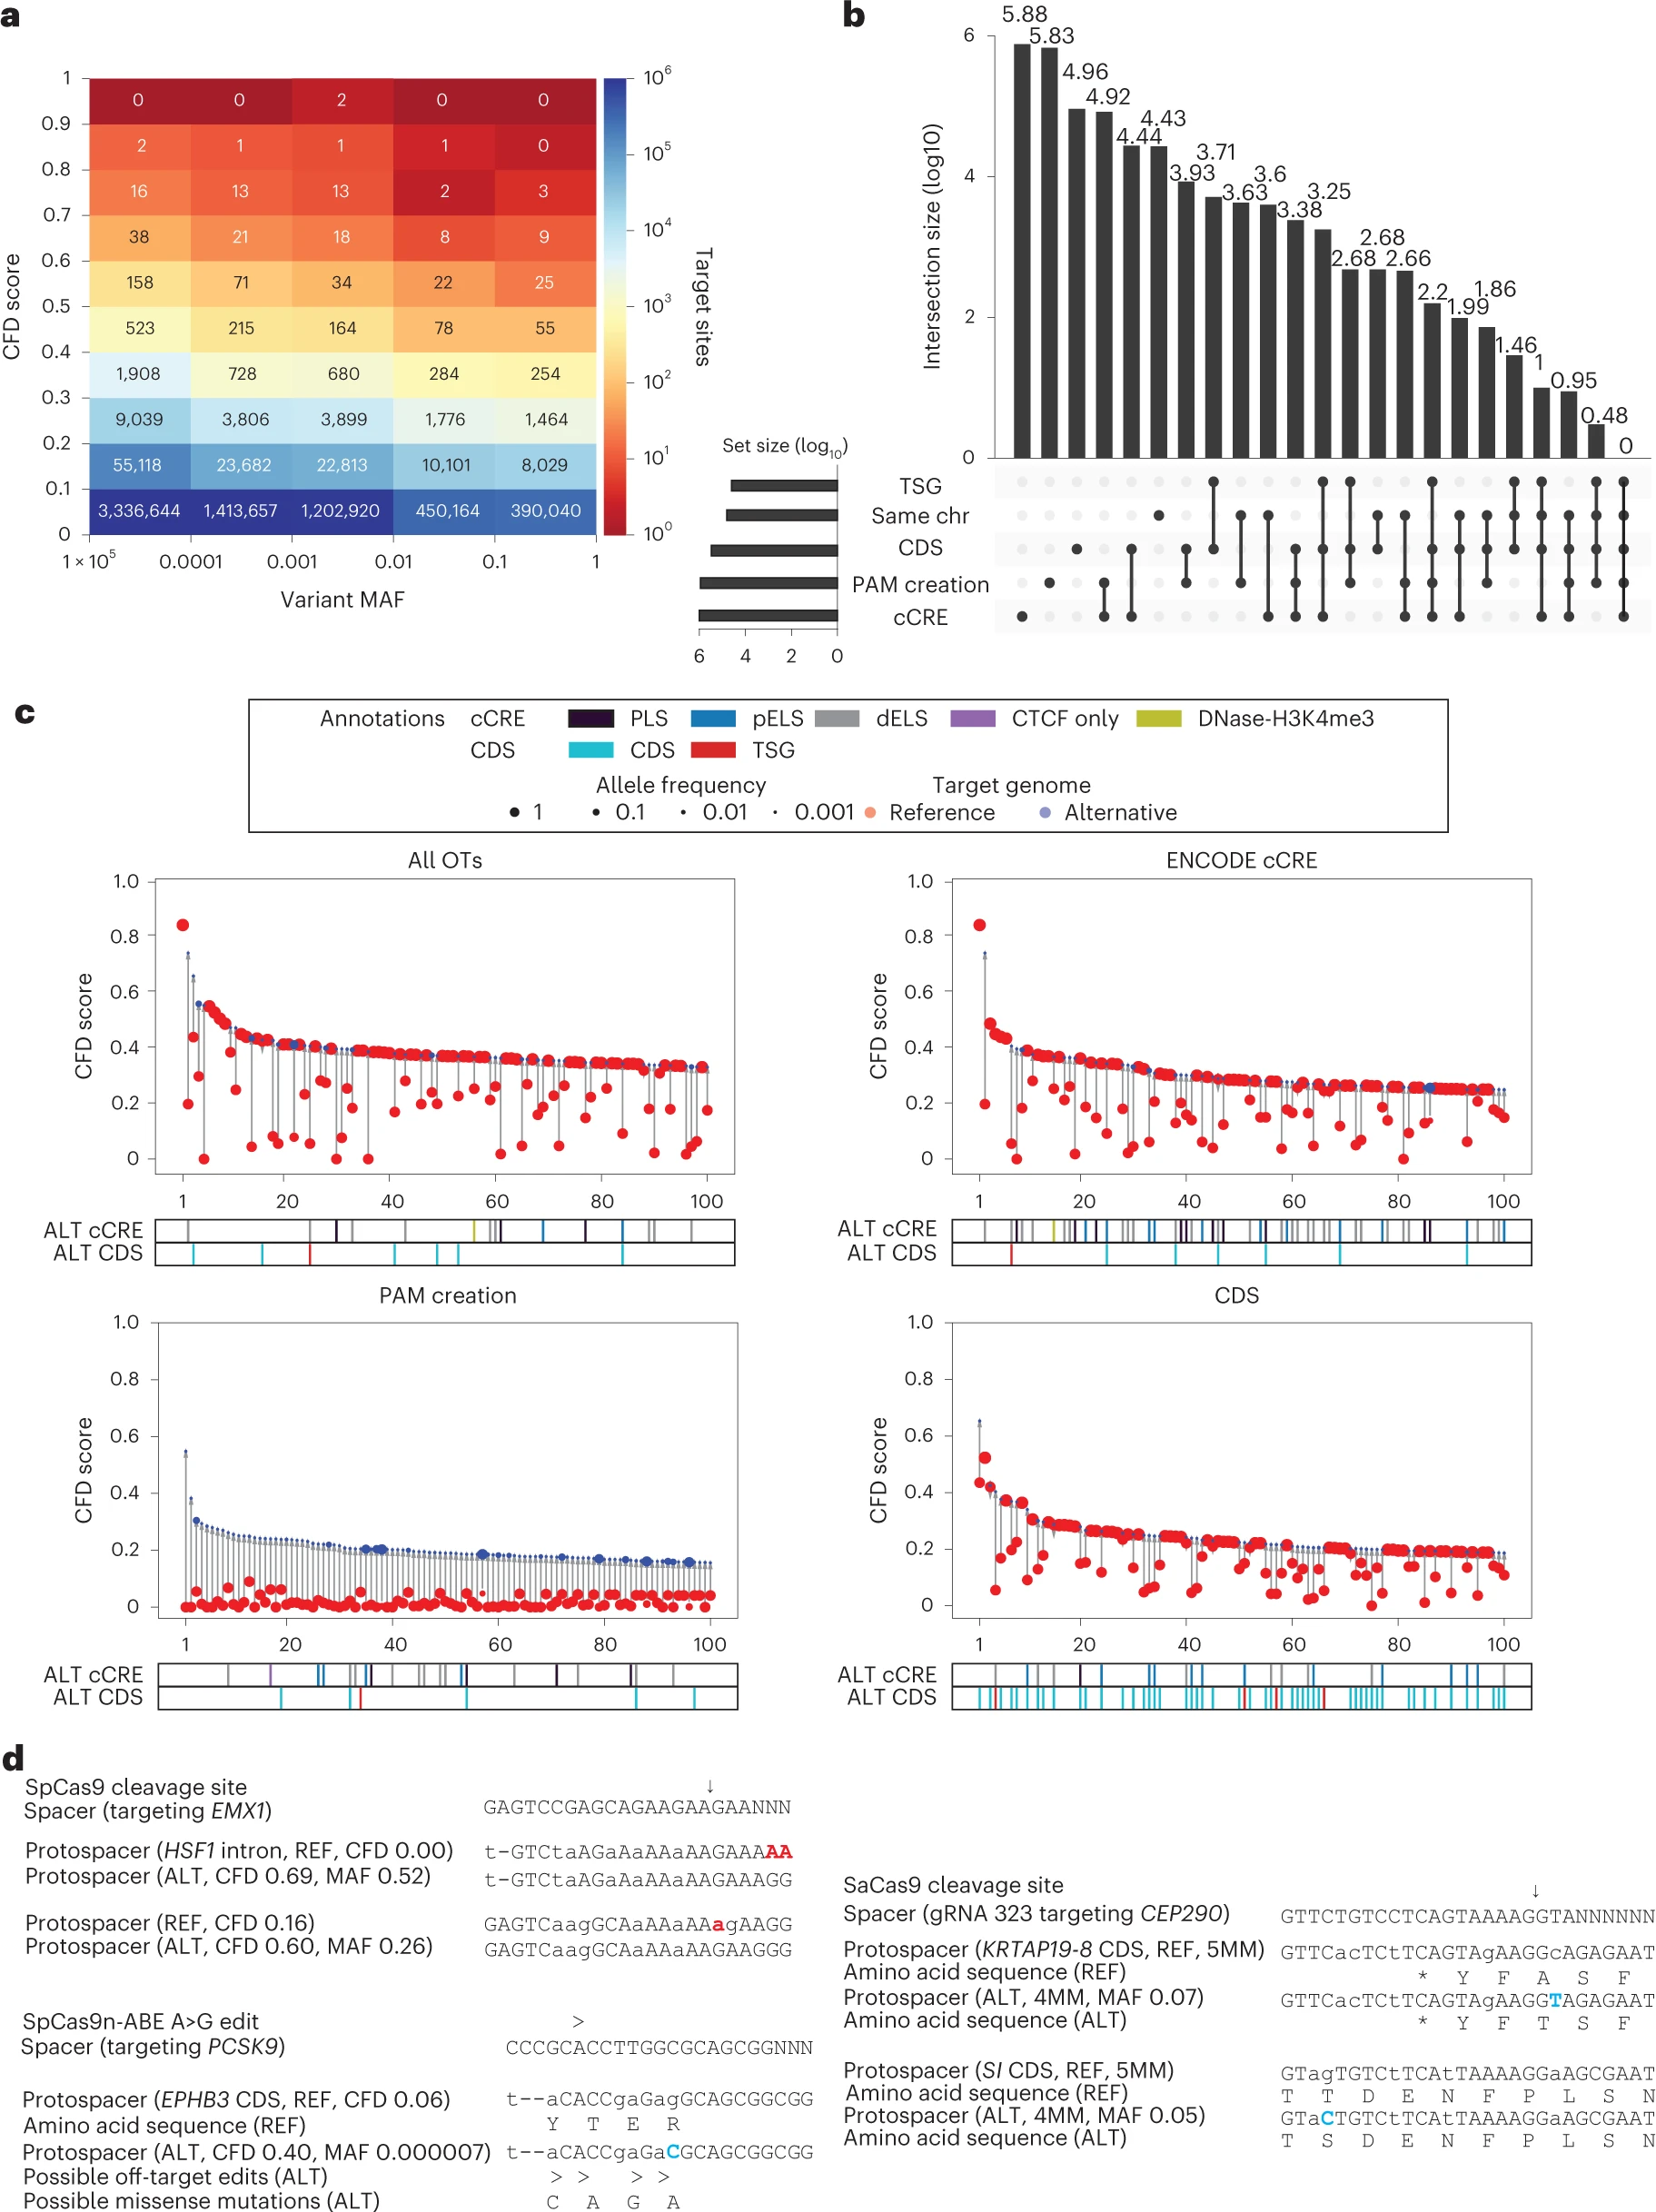
\includegraphics[width=\textwidth]{figures/crisprme8.png}
	\caption[CRISPRme illustrates prevalent off-target potential due to genetic variation]{\textbf{CRISPRme illustrates prevalent off-target potential due to genetic variation (A)} Heatmap showing the distribution of alternative allele nominated off-targets for SpCas9 guides by CFD score and MAF. \textbf{(B)} UpSet plot showing overlapping annotation categories for candidate off-targets (tumor suppressor gene (TSG), candidate off-targets on the same chromosome (chr) as the on-target, CDS regions, cCRE from ENCODE and PAM creation events).  \textbf{(C)} Top 100 predicted off-target sites ranked by CFD score for the gRNA targeting PCSK9 with no filter, found in cCREs, corresponding to PAM creation events, and in CDS regions.\textbf{(D)} Candidate off-target sites with increased predicted cleavage potential introduced by common (MAF 52\% and 26\%) indel variants for a SpCas9 gRNA targeting EMX1 (top left). Candidate off-target cleavage sites within coding sequences with increased homology to a lead gRNA for SaCas9 targeting of CEP290 to treat congenital blindness in current clinical trials due to common SNPs (right). Potential missense mutations in the EPHB3 tumor suppressor resulting from candidate off-target A-to-G base editing by a preclinical lead gRNA targeting PCSK9 to reduce low-density lipoprotein cholesterol levels (bottom). MM denotes mismatches, deletions are shown in red, and SNPs are shown in blue.}
	\label{fig:crisprme8}
\end{figure}
\crisprme can nominate variant off-targets for base editors and evaluate their base editing susceptibility within a user-defined editing window. For a gRNA targeting PCSK9 (ref. 37) that has been used with SpCas9-nickase adenine base editor in vivo in preclinical studies to reduce low-density lipoprotein cholesterol levels, four of the top five candidate off-target sites involve alternative alleles, including one with CFD$_{ref}$ 0.2 and CFD$_{alt}$ 0.75 found in an ENCODE candidate enhancer element. \crisprme nominated a candidate off-target associated with a rare variant (MAF 0.0007\%) that increased the CFD score from 0.06 (REF) to 0.40 (ALT) that would be predicted to produce missense mutations in EPHB3, a putative tumor suppressor gene (\textbf{Fig.\ref{fig:crisprme8}(D)}). The underlying computational challenge that \crisprme addresses extends beyond CRISPR-based applications to other technologies based on nucleic acid sequence recognition. For example, \crisprme can nominate off-targets for RNA-targeting strategies, whether RNA-guided gene editors or even oligonucleotide sequences used as RNA interference or antisense oligo therapies (\textbf{Fig.\ref{fig:crisprme9}}). We performed a variant-aware search (without PAM restriction) for the FDA-approved antisense oligonucleotide Nusinersen \citep{finkel2017nusinersen, mercuri2018nusinersen}, which targets SMN2 pre-mRNA to treat spinal muscular atrophy. Using \crisprme, we identified a potential off-target site within a coding region wherein a common SNP (MAF 2\%) reduces the number of mismatches from three (REF) to two (ALT). Similarly, analysis of the FDA-approved RNA interference therapy Inclisiran \citep{raal2020inclisiran}, which targets PCSK9 mRNA to treat hypercholesterolemia, revealed that its antisense strand has a candidate off-target in the 3' untranslated region of the ribosomal gene RPP14 for which a common insertion variant (MAF 36\%) reduces the number of mismatches and bulges from seven (REF) to four (ALT).
\begin{figure}
	\centering
	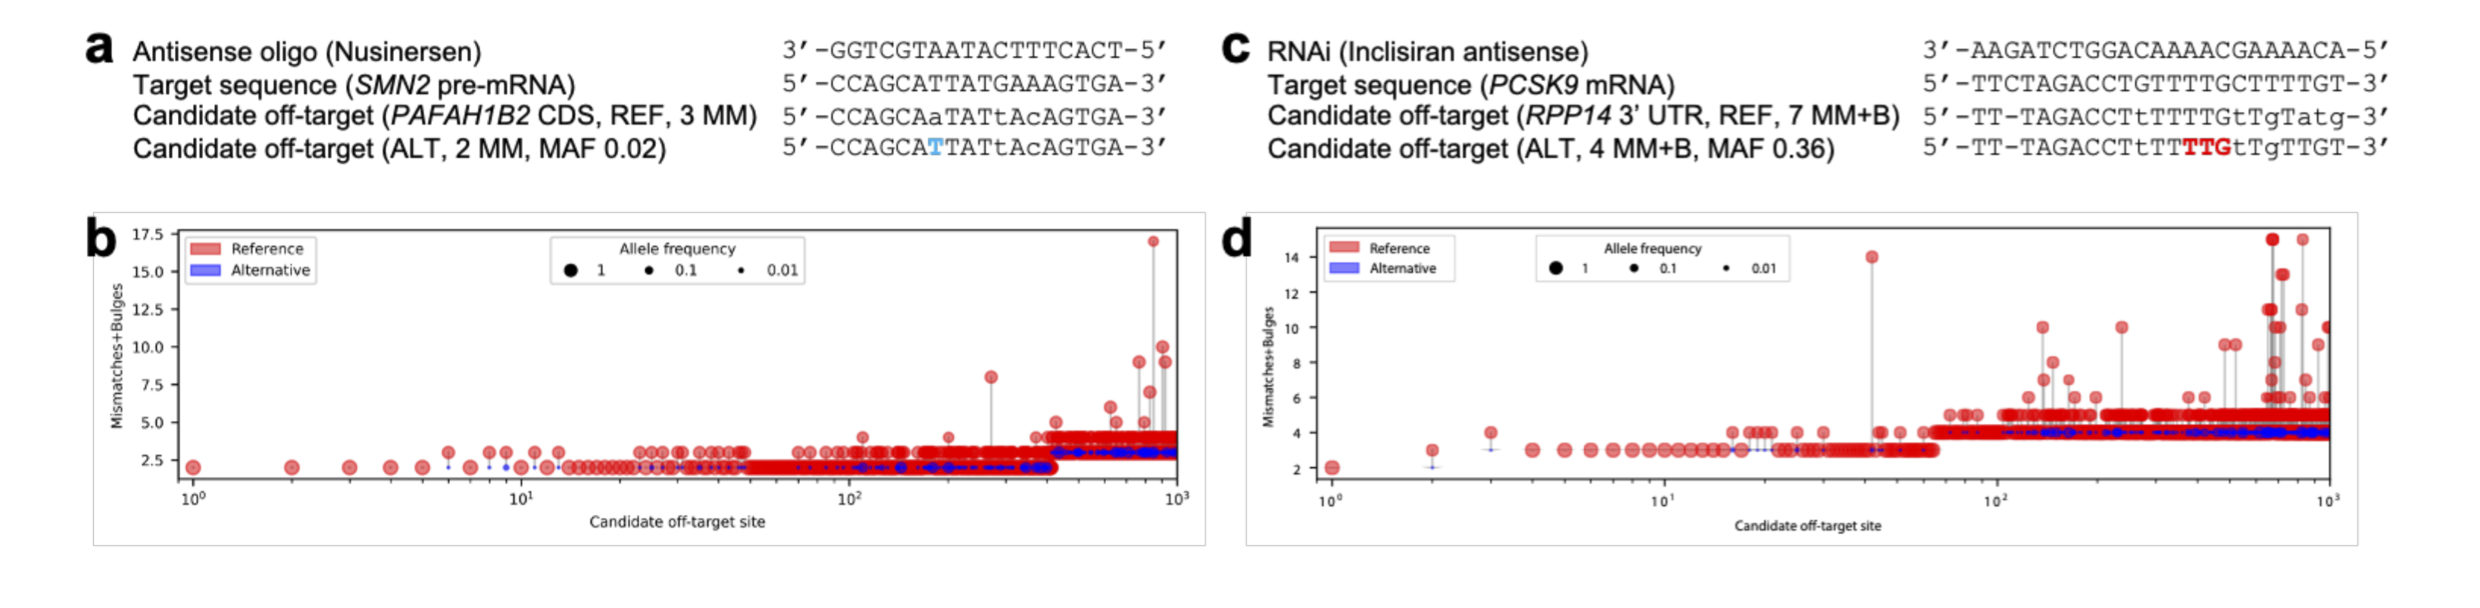
\includegraphics[width=\textwidth]{figures/crisprme9.png}
	\caption[Candidate transcript off-targets introduced by common genetic variants for non-CRISPR sequence-based RNA-targeting therapeutic strategies]{\textbf{Candidate transcript off-targets introduced by common genetic variants for non-CRISPR sequence-based RNA-targeting therapeutic strategies. (A)} A common SNP (in blue) introduces a candidate CDS off-target site with 2 mismatches for the FDA-approved antisense oligo Nusinersen. \textbf{(B)} Top 1000 candidate transcript off-targets ranked by mismatches and bulges for Nusinersen from a search performed with the 1000G and HGDP genetic variant datasets. \textbf{(C)} A common insertion variant (in red) introduces a candidate 3’UTR off-target site with 4 mismatches + bulges for the FDA-approved RNAi therapy Inclisiran. \textbf{(D)} Top 1000 candidate transcript off-targets ranked by mismatches and bulges for Inclisiran from a search performed with the 1000G and HGDP genetic variant datasets.}
	\label{fig:crisprme9}
\end{figure} 
% -- Limitations and Discussion
\subsection{ Limitations and Discussion}
These results demonstrate how personal genetic variation may influence the off-target potential of sequence-based therapies like genome editing. Increased availability of haplotype-resolved genomes of diverse ancestry would enhance ability to nominate variant-associated off-target sites present in human populations. A limitation of current tools including \crisprme is that potential off-targets cannot be enumerated based on structural variants or other complex genetic events such as combinations of indels and SNPs \citep{cancellieri2023human}. Future extensions of CRISPRme based on new data structures such as graph genomes \citep{paten2017genome, garrison2018variation} could enable these complex searches and improve their efficiency. The practical implications of allele-specific off-target editing need to be considered on a case-by-case basis.  In the case of BCL11A enhancer editing, up to $\sim$10\% of SCD patients with African ancestry would be expected to carry at least one rs114518452-C allele, leading to $\sim$10\% cleavage at an off-target site that was not identified in prior studies of this gRNA using currently available tools. Our results highlight that allele-specific off-target editing potential is not equally distributed across all ancestral groups but is especially concentrated in those of African ancestry where genomic variation is most pronounced. Therefore, gene editing efforts that include subjects of African ancestry (like those targeting SCD) might pay particular attention to this issue. Gene editing efforts that focus on a specific patient population should consider genetic variants enriched in that population during off-target evaluation. However, our analysis also shows that variant off-targets may be private to a given individual, so all humans could potentially be susceptible to such an effect. Implementing off-target analysis and testing into therapeutic genome editing protocols in practice is an important issue that is broader in scope than our report. Fundamentally, variant-aware off-target analysis may identify off-target potential that would be overlooked by conventional analysis. Of note, as is true for off-target genetic changes in general, the mere possibility of somatic genetic alteration does not imply functional consequence. Although in principle, ex vivo-edited patient cells could be tested by sequencing before infusion, the functional importance of off-target edits may range from likely functional to likely neutral, so the mere presence of off-target editing in a cell product may not necessarily preclude its clinical use, and this testing could deplete precious material and delay therapy. We recommend several steps to minimize risk of unintended allele-specific off-target effects during therapeutic genome editing, consistent with regulatory guidance to consider effects of genetic variation. First, prioritize use of genome editing methods that maximize specificity, such as high-fidelity editors and pulse delivery. Second, nominate off-targets in a variant-aware manner, with particular attention toward genetic variants found in relevant patient populations, using a tool like \crisprme \citep{cancellieri2023human}. Third, use off-target detection assays that are variant-aware to empirically evaluate the likelihood of off-target editing, although these may imperfectly reflect editing in a therapeutic context (Supplementary Note 7). When possible, allele-specific off-target editing potential should be validated in primary cells of relevant genotype by sequencing. However, it may be difficult to obtain such primary cells to perform biological validation in a relevant therapeutic context. Fourth, perform a risk assessment of variant off-target editing given predicted genomic annotations, mechanisms of DNA repair, delivery to target cells and disease context. For example, off-target edits within tumor suppressor loci might carry greater risk than those targeting unannotated non-coding sequences. Fifth, if excess allele-specific genome editing risks are identified, consider including genotype among the subject inclusion/exclusion criteria. Finally, for therapeutic genome editing indications in which it is feasible (such as hematopoietic cell targeting), prospectively monitor somatic modifications in patient samples to gather information about the frequency and consequence of such events to help assess patient-specific risk and provide valuable information for the broader field as to the frequency and in vivo dynamics of off-target edits if present.\crisprme offers a simple-to-use tool to comprehensively evaluate off-target potential across diverse populations and within individuals. \crisprme is available at \url{http://crisprme.di.univr.it} and may also be deployed locally to preserve privacy.
% ------ Joint genotypic and phenotypic outcome modeling improves base editing variant effect quantification 
\section{Joint genotypic and phenotypic outcome modeling improves base editing variant effect quantification}
Genetic variation contributes substantially to complex disease risk. While well-powered genome-wide association studies (GWAS) \citep{tam2019benefits}and rare variant analyses from cohort studies such as the UK Biobank (UKB) \citep{bycroft2018uk} have associated thousands of loci and genes with clinical phenotypes, these observational approaches are often insufficient to identify causal variants. Perturbation-based methods enable evaluation of the impact of an individual variant in a common genetic background, isolated from genetically linked variants, and such testing can be performed in high throughput through multiplex assays of variant effect (MAVEs) \citep{gasperini2016power}. Numerous types of MAVEs have been developed, including deep mutational scanning (DMS) \citep{araya2011deep},  saturation mutagenesis \citep{myers1986fine}, massively parallel reporter assays (MPRA) \citep{inoue2015decoding},  and CRISPR-based screens \citep{bock2022high, shalem2014genome, wang2014genetic}.  CRISPR base editing screens have emerged as a uniquely powerful method to study variants in their endogenous genomic context. Base editors, fusions of Cas9-nickase and single-stranded cytosine or adenine deaminase enzymes \citep{komor2016programmable, gaudelli2017programmable},enable site-specific installation of transition variants. As the majority of disease-associated variants are single-nucleotide transitions citep{rees2018base}, base editors enable the installation of functionally relevant variants in a precise and scalable way. Base editing screens have been employed to dissect coding variant effects as well as to evaluate GWAS-associated variant functions \citep{hanna2021massively, morris2023discovery, martin2023massively, cuella2021functional, pablo2023scanning, coelho2023base, cheng2021single, sanchez2022base, kim2022high, kweon2020crispr, huang2021identification, sangree2022benchmarking, lue2023base, despres2020perturbing, garcia2023base, lue2023base}. However, base editing efficiency varies substantially depending on the local sequence context surrounding the target base, the specific Cas9 variant and deaminase used, and the cellular context \citep{arbab2020determinants}. Moreover, base edits can occur at multiple positions within the single-stranded DNA bubble created by the guide RNA (gRNA)-DNA binding on the opposite strand, therefore a single gRNA can install a variety of alleles, each with distinct efficiencies. While there have been efforts to predict editing outcomes using massively parallel base editor reporter assay data \citep{arbab2020determinants}, these predictions do not generalize well to unprofiled base editors and cellular contexts \citep{sanchez2022base}. In previous base editing screens, analysis of phenotypic outcomes is confounded by variable editing efficiencies and outcomes. Phenotypic effects of gRNAs with robust editing are exaggerated, and effects of variants that are not installed as efficiently are underestimated. Such confounding is especially pernicious when the target elements are coding variants, as a single gRNA may install distinct coding variants with different frequencies, and current analysis methods are unable to deconvolve such data.  Existing base editing screens have dealt with the heterogeneity in gRNA efficiency and genotypic outcomes in several ways. One approach that has been employed is to assume all editable nucleotides within the editing window are edited with uniform efficiency \citep{hanna2021massively}. Two recent studies have profiled the gRNAs used in phenotypic base editing screening using a base editor reporter (or sensor) assay \citep{sanchez2022base, kim2022high} to filter gRNAs with low editing efficiency when analyzing their phenotypic data. Despite these initial efforts, the computational analyses of these screens have not yet been formalized, often relying on existing tools that were not designed specifically for base editor data with or without the target site reporter. Here, we design an experimental-computational pipeline to improve the accuracy of variant effect estimation in base editing screens. By incorporating a target site reporter sequence into the gRNA construct, we simultaneously measure the editing efficiency of a gRNA and its phenotypic impact. We develop a computational pipeline, BEAN, that normalizes the phenotypic scores of target variants using genotypic outcome information collected from the target site reporter. Moreover, we extend BEAN to analyze densely tiled coding sequence base editing screen data, sharing information among neighboring gRNAs to obtain accurate phenotypic scores for each coding variant. BEAN provides a first-in-class integrated solution to experimental assessment of variant effects through base editing screens. We systematically benchmark BEAN against current state-of-the-art methods for the analyses of pooled CRISPR screens and show substantially improved performance of BEAN. To leverage activity-normalized base editing screening, we have conducted screens assessing the impact of low-density lipoprotein cholesterol (LDL-C)-associated GWAS variants and low-density lipoprotein receptor (LDLR) coding variants on LDL-C uptake in HepG2 hepatocellular carcinoma cells. Genetic differences in LDL-C levels contribute substantially to coronary artery disease risk. Serum LDL-C measurements are quantitative and nearly uniformly measured in most biobanks, and thus they provide among the highest quality human phenotypic data for any trait. A trans-ancestry GWAS meta-analysis from the Global Lipids Genetics Consortium (GLGC) has identified $>$900 genome-wide significant loci associated with blood lipid levels, including $>$400 loci associated with LDL-C \citep{graham2021power}. LDL-C GWAS loci overlap strongly with liver-enriched gene expression, nominating liver as the primary tissue driving LDL-C variant effects \citep{wang2022epic, finucane2018heritability}. Yet, the causal variants and mechanisms by which many of these loci modulate LDL-C levels remain unknown.  LDL-C levels are also impacted by rare coding variants. In the most severe instances, inherited monogenic variants in several genes cause Familial Hypercholesterolemia (FH), a disease associated with extremely elevated LDL-C levels and premature cardiovascular disease \citep{bouhairie2015familial}. The majority of genetic mutations known to cause FH occur in LDLR, a cell surface receptor that uptakes LDL, thus removing it from circulation \citep{brown1984ldl} Despite the effectiveness of lipid lowering therapies, FH patients are still 2-4-fold more likely to have coronary events than the general population \citep{mundal2018impact}. Elevated LDL-C levels increase cardiovascular disease risk throughout life, so the early identification of at-risk individuals would have immense clinical utility \citep{bouhairie2015familial}. However, many LDLR variants currently lack clinical interpretation. Of the 1,427 LDLR missense variants in the ClinVar databasen \citep{landrum2020clinvar}, 50\% are classified as variants of unknown significance (VUS) or to have conflicting interpretations of pathogenicity (“conflicting”), thus impeding FH diagnosis. Likewise, of the 758 unique LDLR missense variants carried by sequenced individuals in the UKB cohort, 69\% are either unreported or have an uncertain annotation in ClinVar. Altogether, improved understanding of LDLR variant impacts would enable earlier diagnosis and treatment for a large number of at-risk individuals. We have modeled the impacts of both common GWAS-associated and rare LDLR coding variants through base editing installation followed by cellular uptake of fluorescent LDL-C in HepG2 cells, which provides a scalable flow cytometric assay to measure a key contributing factor of serum LDL-C levels \citep{hamilton2023systematic} given the majority of serum LDL-C is cleared in liver \citep{spady1992hepatic}.  By applying our experimental-computational pipeline to this screen model, we identify LDL uptake-altering GWAS-associated variants and characterize their downstream impact on chromatin accessibility, transcription factor binding, and gene expression that leads to differential LDL uptake. We nominate causal variants that alter LDL-C uptake through impacting the genes  OPRL1, VTN, and ZNF329, which have not previously been connected with LDL-C levels. Through saturation tiled base editing of LDLR, not only do we accurately distinguish known pathogenic vs. benign variants, we find strong correlation between missense variant functional scores and the LDL-C levels of patients in the UKB who carry these variants. We combine functional scores with structural modeling to mechanistically classify deleterious variant impacts, revealing a key, conserved tyrosine residue in each LDLR class B repeat that interacts with the neighboring repeat to maintain structural integrity. Altogether, BEAN provides a widely applicable tool to characterize single-nucleotide variant functions. 
% ---- A base editing reporter profiles endogenous editing outcomes
\subsection{A base editing reporter profiles endogenous editing outcomes}
\begin{figure}
	\centering
	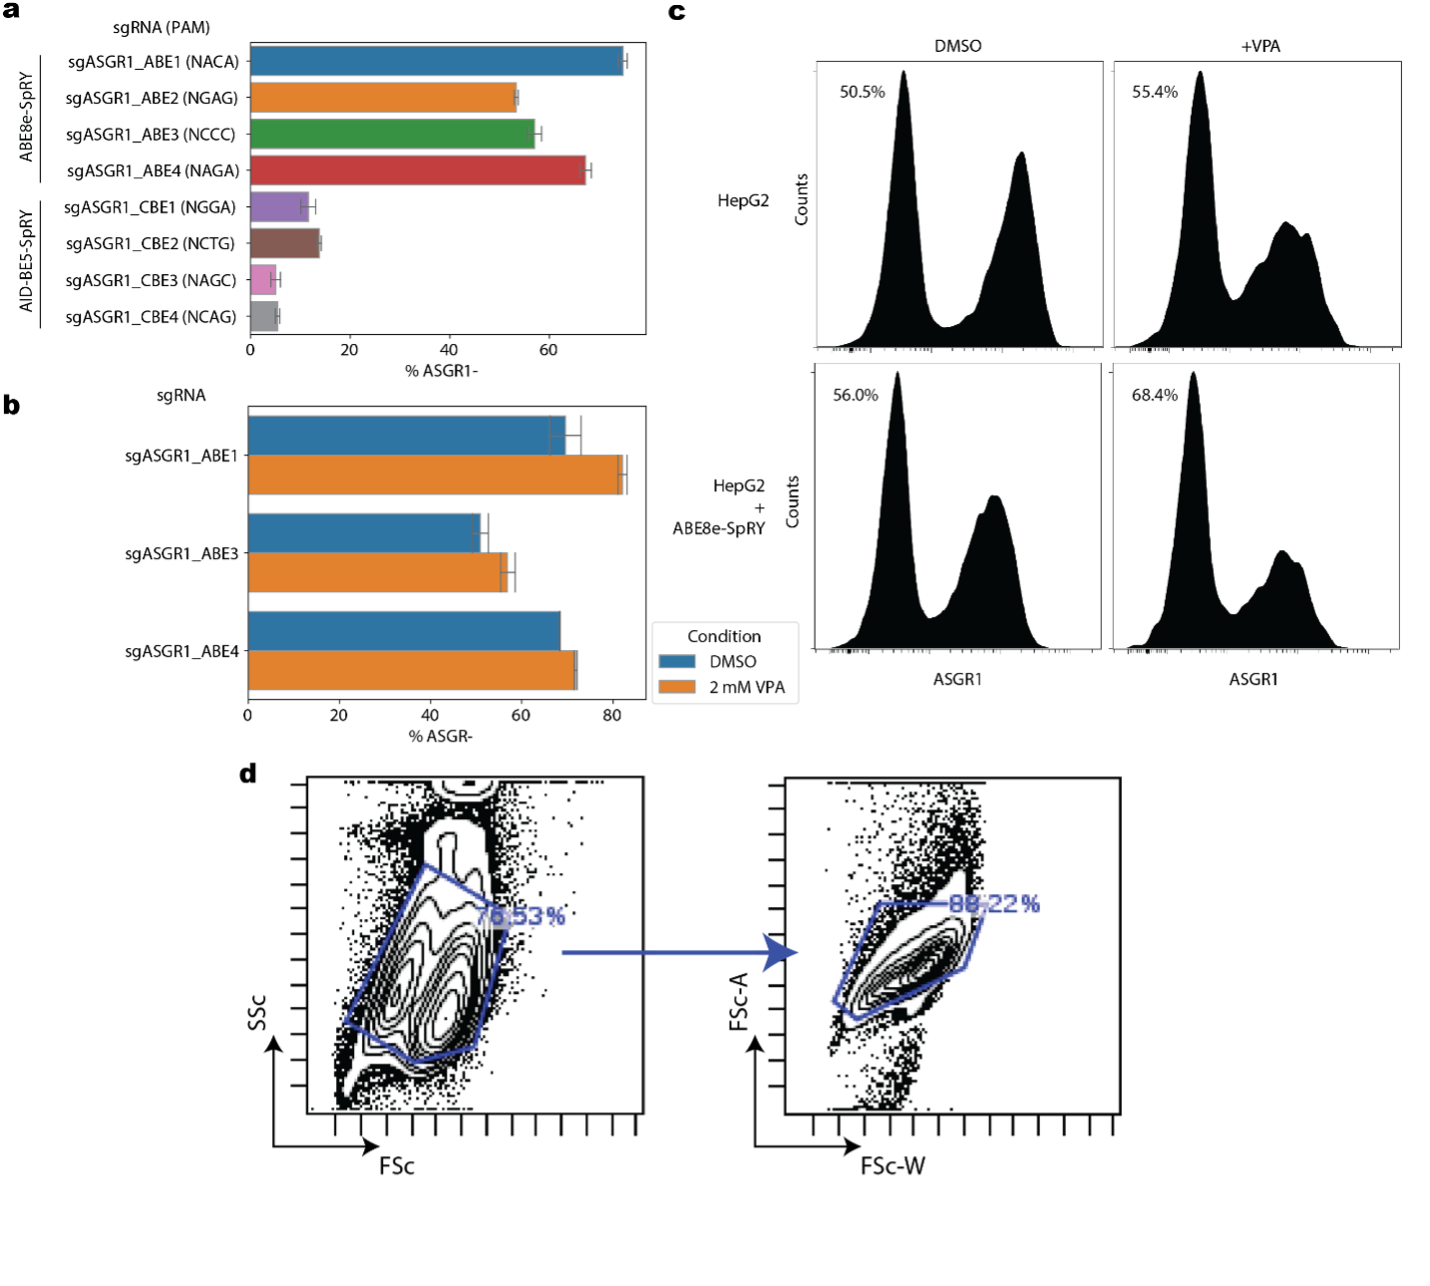
\includegraphics[width=\textwidth]{figures/crisprbean1.png}
	\caption[Optimization of SpRY base editing]{\textbf{Optimization of SpRY base editing. (A)} ) gRNA editing efficiency in HepG2 with ABE8e-SpRY and AID-BE5-SpRY for ASGR1 splice site-targeted gRNAs, measured by the fraction of ASGR1 negative cell counts (\% ASGR -) quantified by flow cytometry from two experimental replicates. \textbf{(B)} gRNA editing efficiency with and without valproic acid (VPA) treatment from 4 experimental replicates. \textbf{(C)} Flow cytometry signal with and without stable ABE8e-SpRY integration and valproic acid (VPA) treatment. Fraction of ASGR negative cell counts in each condition is labeled as percentage in the panel.  \textbf{(D)} Example flow cytometric gates used in all analysis and sorting experiments to filter for single cells. }
	\label{fig:crisprbean1}
\end{figure} 
To enable accurate interrogation of variant effects at scale, we built a platform to perform dense, high-coverage base editing screens that accounts for variable editing efficiency and genotypic outcomes. To maximize coverage of variants in base editing screens, we built lentiviral adenine (ABE8e) \citep{gaudelli2017programmable, richter2020phage} and cytosine (AID-BE5) \citep{arbab2020determinants} deaminase base editor (BE) constructs using the near-PAM-less SpCas9 variant, SpRY \citep{walton2020unconstrained}. Both BEs showed native genomic editing activity, as measured in HepG2 cells by ASGR1 splice site editing followed by flow cytometric anti-ASGR1 antibody staining, with ABE8e-SpRY showing considerably more robust maximal activity (\textbf{Fig.\ref{fig:crisprbean1}(A)}). Editing efficiency was increased by 5-10\% by prior lentiviral integration of constitutively expressed BEs and by transient dosing of cells with the histone deacetylase valproic acid immediately after BE and gRNA transduction (\textbf{Fig.\ref{fig:crisprbean1}(B)-(C)}), and thus these treatments were implemented in all screens.Base editing efficiency is known to vary depending on Cas9 binding efficiency as well as the local sequence and chromatin context surrounding the target base \citep{arbab2020determinants, shin2021small, yang2023hmgn1}, and thus we expected gRNAs to vary substantially in editing efficiency across target sites. To account for this variability, we synthesized and cloned each gRNA paired with a 32-nt reporter sequence comprising the genomic target sequence of that gRNA into lentiviral base editor vectors (\textbf{Fig. \ref{fig:crisprbean2}(A)}), akin to previously published CRISPR mutational outcome reporter constructs \citep{sanchez2022base, kim2022high}. When introduced into cells, the gRNA can edit both its native genomic target site and the adjacent target site (reporter) in the lentiviral vector, which can be read out using next-generation sequencing (NGS). 
\begin{figure}
	\centering
	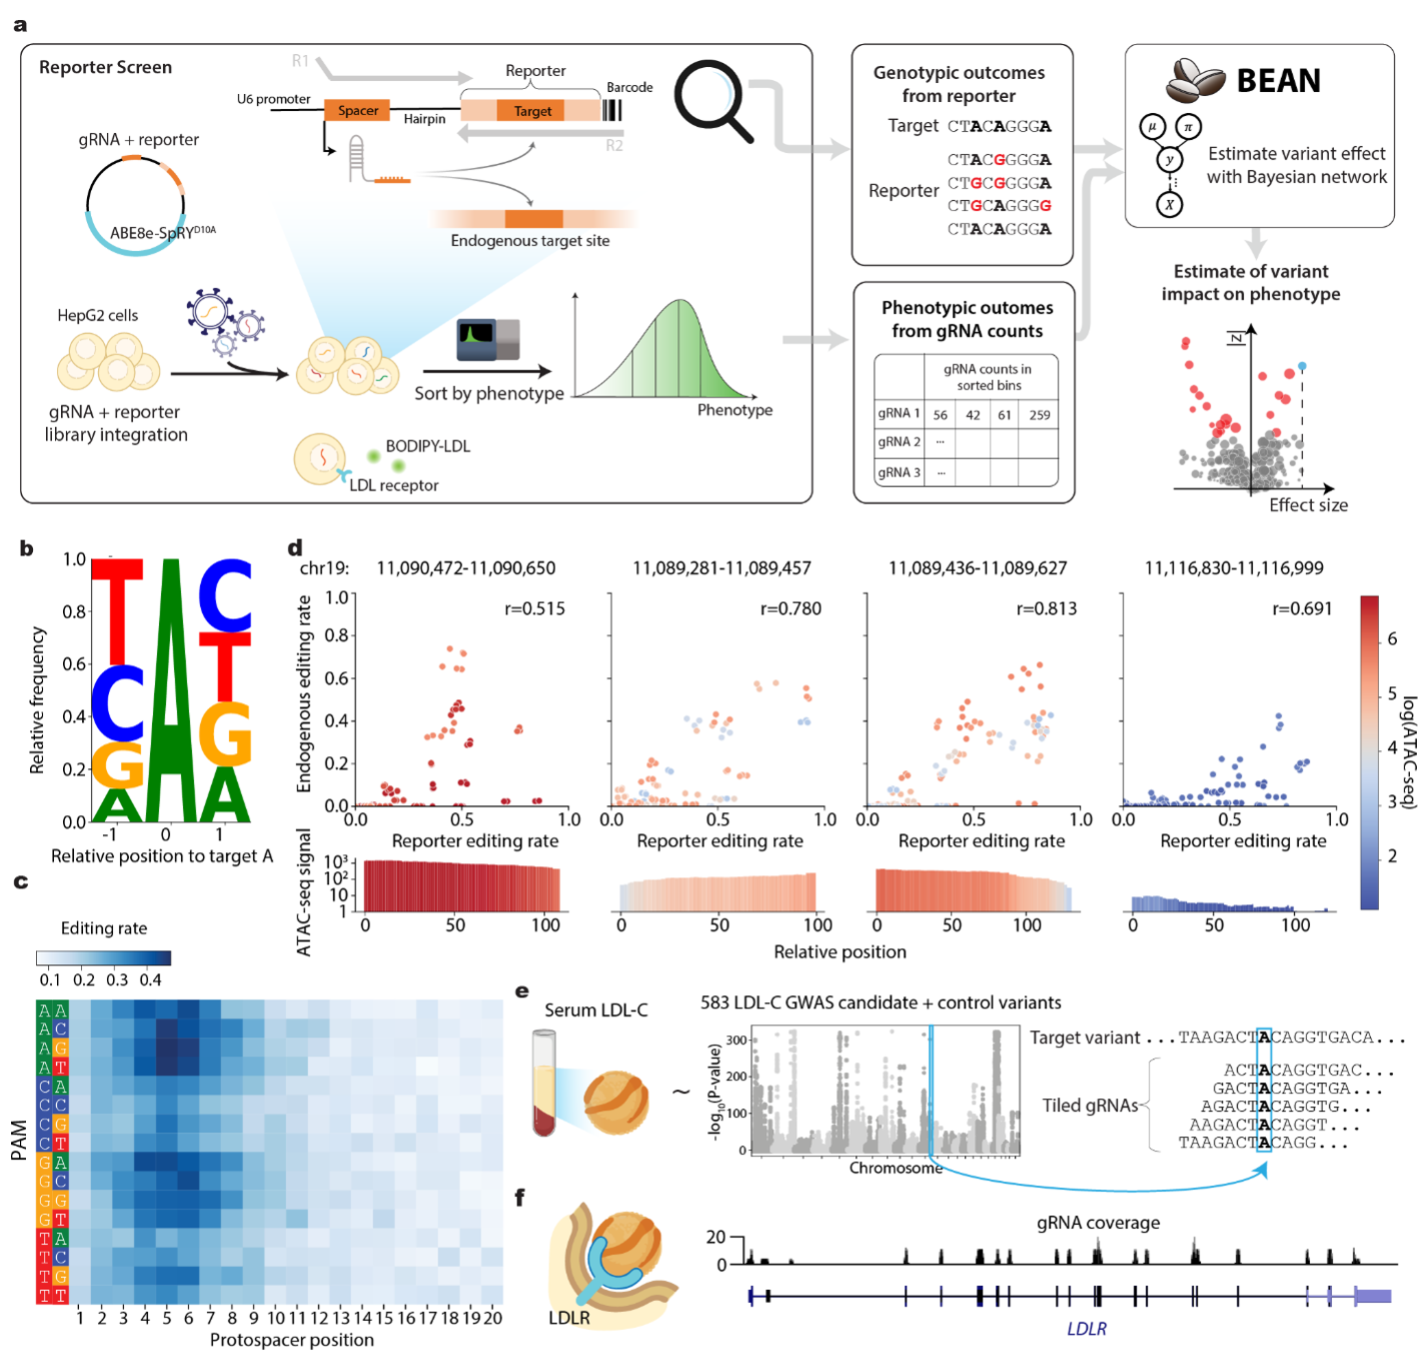
\includegraphics[width=\textwidth]{figures/crisprbean2.png}
	\caption[Activity-normalized base editing screening pipeline]{\textbf{Activity-normalized base editing screening pipeline. (A)} ) Schematic of activity-normalized base editing screening process and analysis by BEAN. A library of gRNAs, each paired with a reporter sequence encompassing its genomic target sequence, is cloned into a lentiviral base editor expression vector. Lentiviral transduction is performed in HepG2, followed by flow cytometric sorting of four populations based on fluorescent LDL-cholesterol (BODIPY-LDL) uptake. The gRNA and reporter sequences are read out by paired-end NGS to obtain gRNA counts and reporter editing outcomes in each flow cytometric bin. BEAN models the reporter editing frequency and allelic outcomes and gRNA enrichments among flow cytometric bins using BEAN to estimate variant phenotypic effect sizes. \textbf{(B)} Adjacent nucleotide specificity of ABE8e-SpRY editing represented as a sequence logo from 7,320 gRNAs; the height of each base represents the relative frequency of observing each base given an edit at position 0.  \textbf{(C)} Average editing efficiency of ABE8e-SpRY by protospacer position and PAM sequence \textbf{(D)} Scatterplots comparing nucleotide-level editing efficiency between the reporter and endogenous target sites for a total of 49 gRNAs across four loci across 3 experimental replicates. The accessibility of the four loci as measured by ATAC-seq signal in HepG2 is shown in the top panel, and the scatterplot markers are colored by the accessibility of each nucleotide. Pearson correlation coefficients are shown as $r$. \textbf{(E)} Schematic of the LDL-C variant library gRNA design for selected GWAS candidate variants with a Manhattan plot showing variant P-values from a recent GWAS study \citep{klimentidis2020phenotypic}.  gRNAs tile the variant at five positions with maximal editing efficiency (protospacer positions 4-8).  \textbf{(F)} gRNA coverage of the LDLR tiling library across LDLR coding sequence along with 5’ and 3’ UTRs and several regulatory regions. }
	\label{fig:crisprbean2}
\end{figure} 
We designed two gRNA libraries using this approach to improve understanding of the genetics of LDL-C levels. The first library (LDL-C GWAS library) targets 583 variants associated with LDL-C levels from the UK Biobank GWAS cohort. We included fine-mapped variants with posterior inclusion probability (PIP) $>$0.25 from either the SUSIE or Polyfun fine-mapping pipelines \citep{wang2020simple, weissbrod2020functionally}, and also variants with PIP $>$ 0.1 within 250 kb of any of 490 genes found to significantly alter LDL-C uptake from recent CRISPR-Cas9 knockout screens \citep{hamilton2023systematic, emmer2021genome}. We designed five tiled gRNAs for each variant allele that place the variant in positions shown to induce most efficient editing with ABE8e (\textbf{Fig. \ref{fig:crisprbean2}(E)}) \citep{arbab2023base}. Positive control gRNAs which ablate splice donor and acceptor consensus sites in six genes found to have significantly altered LDL-C uptake upon knockout \citep{hamilton2023systematic} and 100 non-targeting negative control gRNAs that tile 20 synthetic variants were included, for a total of 3,455 gRNAs.The second library (LDLR tiling library) targeted the LDLR gene. Taking advantage of the flexible PAM recognition of SpRY, every possible gRNA targeting the LDLR coding sequence on both strands was included. Lower density gRNAs, tiled every 2-3-nt, targeted the the 50-nt flanking each LDLR exon, the LDLR 5’ and 3’ UTR, promoter, and two intronic enhancers (\textbf{Fig. \ref{fig:crisprbean2}(F)}). This library also contained 150 non-targeting negative control gRNAs, for a total of 7,500 gRNAs.We first assessed editing outcomes through lentiviral transduction of each library in HepG2 cells followed by NGS of gRNA-reporter pairs 10-14 days afterwards. We developed an end-to-end computational toolkit for base-editing screens, BEAN, which includes the ability to perform quality control and quantify editing outcomes from raw reads among other functionalities. Importantly, the quantification step is designed to account for self-editing of the spacer sequence, which we found to occur at appreciable frequency and with modest correlation with reporter editing frequency (LDL-C GWAS library median 31\%, Pearson $r$=0.36, LDLR tiling library median 18\%, $r$=0.31). We used BEAN to profile the previously uncharacterized PAM-less base editors ABE8e-SpRY and AID-BE5-SpRY on reporter data from the $>$10,000 gRNAs in both libraries (\textbf{Fig.\ref{fig:crisprbean2}(B)} and \textbf{(C)}),. The result clearly recapitulated the hallmark positional preferences of these base editors \citep{myers1986fine, wang2014genetic} the NRY PAM preference of the SpRY enzyme \citep{komor2016programmable, gaudelli2017programmable}, and the relative depletion of editing at AA dinucleotides by ABE8e. Notably, the average maximal positional ABE8e-SpRY editing frequency at protospacer positions 3-8 across dinucleotide PAM sequences ranges from 32\% to 46\%, indicating the ability of this enzyme to install variants efficiently across a wide variety of genomic locations.To validate that editing of the reporter provides an accurate surrogate for endogenous editing, we generated a library where both the reporter and endogenous target site are sequenced following the editing by 49 gRNAs across four loci surrounding LDLR with varying levels of HepG2 chromatin accessibility. We demonstrate that nucleotide-level and allele-level reporter editing fractions correlate well with endogenous target site editing fractions ((\textbf{Fig.\ref{fig:crisprbean2}(D)}, average Pearson correlation across 4 loci is $r$=0.70 for per-nucleotide editing rate $r$=0.70, per-allele editing rate $r$=0.69), and the reporter shows higher correspondence than BE-Hive predictions29 (Nucleotide $r$=0.44, allele $r$=0.64) (\textbf{Fig.\ref{fig:crisprbean3}}). Notably, while reporter editing correlates with endogenous editing at all four loci, we found that endogenous editing frequency also depends on the accessibility of the target region, as has been previously reported for Cas9-nuclease \citep{schep2021impact, ding2019improving, liu2019modulating} and base editors \citep{shin2021small, yang2023hmgn1}. Yet, current computational analyses do not model these dependencies, motivating the development of a tailored modeling framework.
\begin{figure}
	\centering
	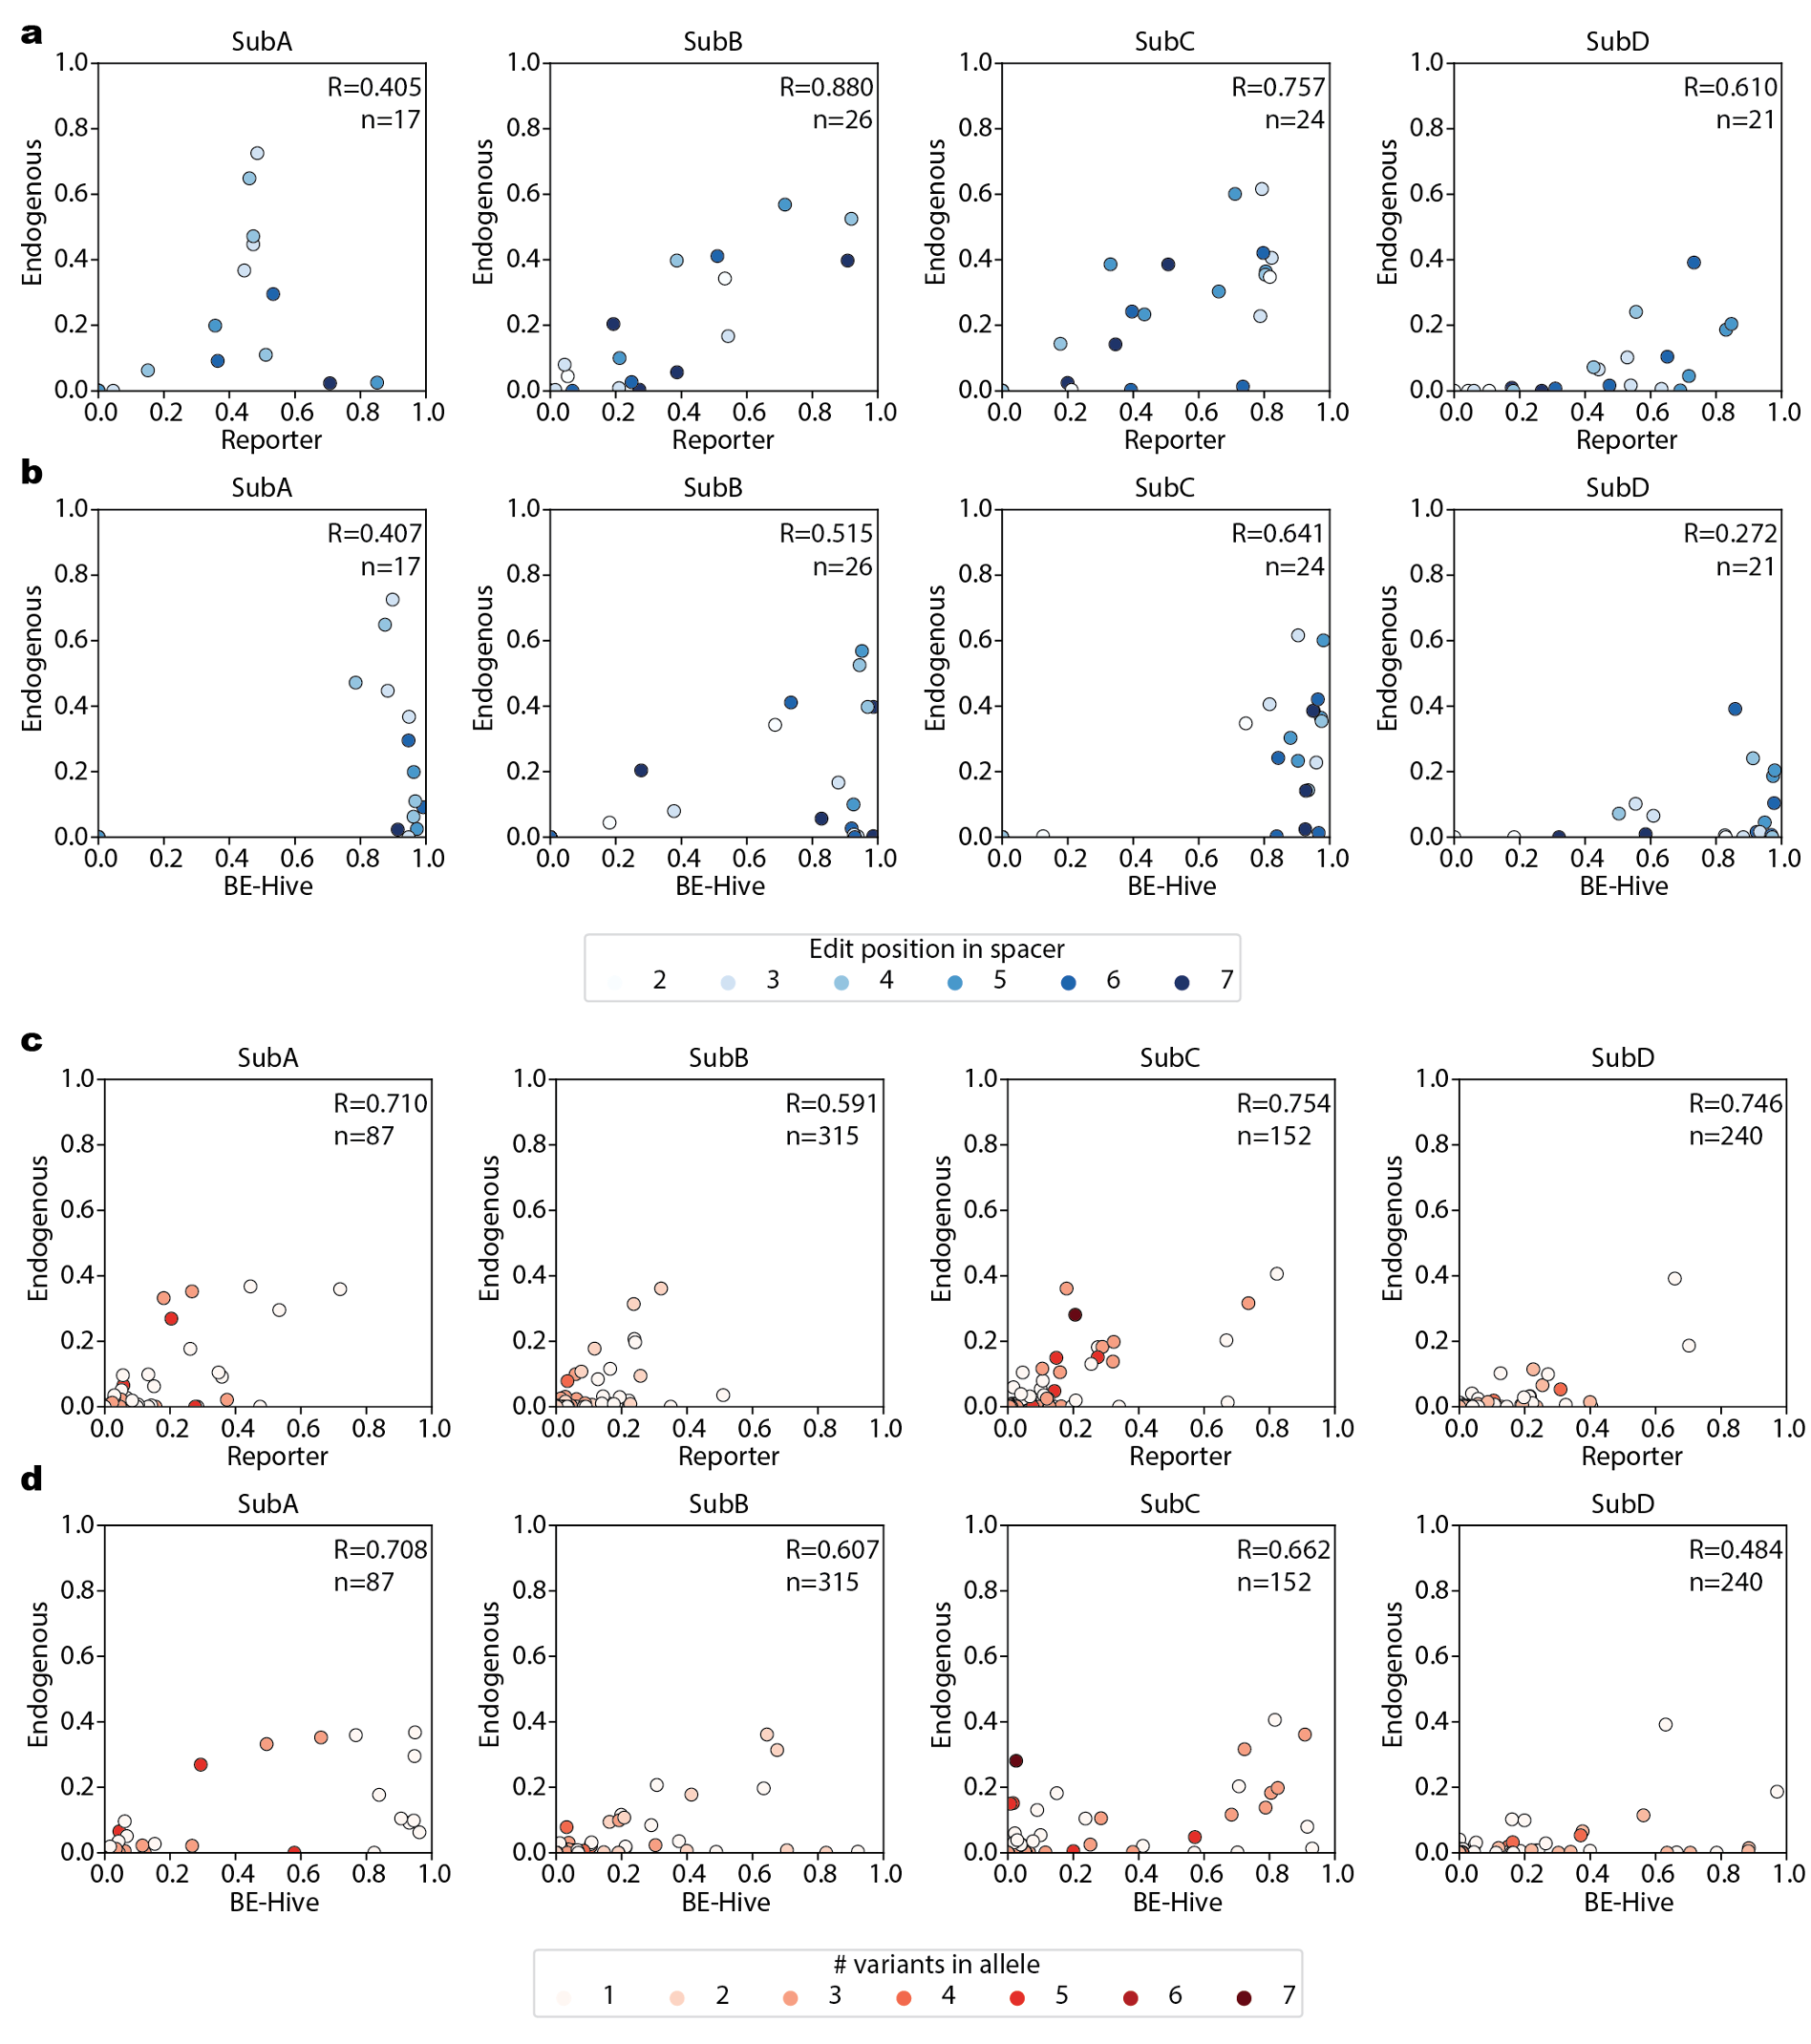
\includegraphics[width=\textwidth]{figures/crisprbean3.png}
	\caption[Endogenous target site editing rate comparison with reporter and BE-Hive predicted editing outcomes]{\textbf{Endogenous target site editing rate comparison with reporter and BE-Hive predicted editing outcomes. } Mean endogenous and reporter edit rates across three replicates are plotted. \textbf{(A)-(B)} Nucleotide-level editing rates in \textbf{(A)} reporter and \textbf{(B)} BE-Hive plotted against those in endogenous loci within protospacer position 2 to 7 (1-based, inclusive). \textbf{(B)} Allele level editing rates in \textbf{(C)} reporter and \textbf{(D)} BE-Hive plotted against those in endogenous loci. Alleles are defined within editing window within protospacer 1 to 19 (1-based, inclusive). SubA-D denotes sublibraries A-D. Pearson correlation coefficients are denoted as R and the number of points is denoted as n.}
	\label{fig:crisprbean3}
\end{figure} 
We then performed fluorescent LDL uptake screens with each library in $\geq$ 5 biological replicates, ensuring $>$500 cells per gRNA at all stages. We used simulation to determine the optimal flow cytometric sorting scheme, accounting for variability in gRNA editing rate, gRNA coverage, gDNA sampling and PCR amplification (\url{https://github.com/pinellolab/screen-simulation}). Based on our simulation result that finer bin widths improves sensitivity (Supplementary Fig. 6, Supplementary Note 1), we flow cytometrically isolated four populations per replicate with the very low (0-20\% percentile), low (20-40\%), high (60-80\%), and very high (80-100\%) LDL uptake (\textbf{Fig.\ref{fig:crisprbean2}(A)}), performing NGS on gRNA and reporter pairs in each sorted population. We observed robust replicability (median Spearman $\rho$=0.84 for LDL-C GWAS library, 0.88 for LDLR tiling library) in gRNA counts across replicates (Supplementary Fig. 7), indicating technical reproducibility.  the variant at five positions with maximal editing efficiency (protospacer positions 4-8). f) gRNA coverage of the LDLR tiling library across LDLR coding sequence along with 5’ and 3’ UTRs and several regulatory regions. 
\begin{figure}
	\centering
	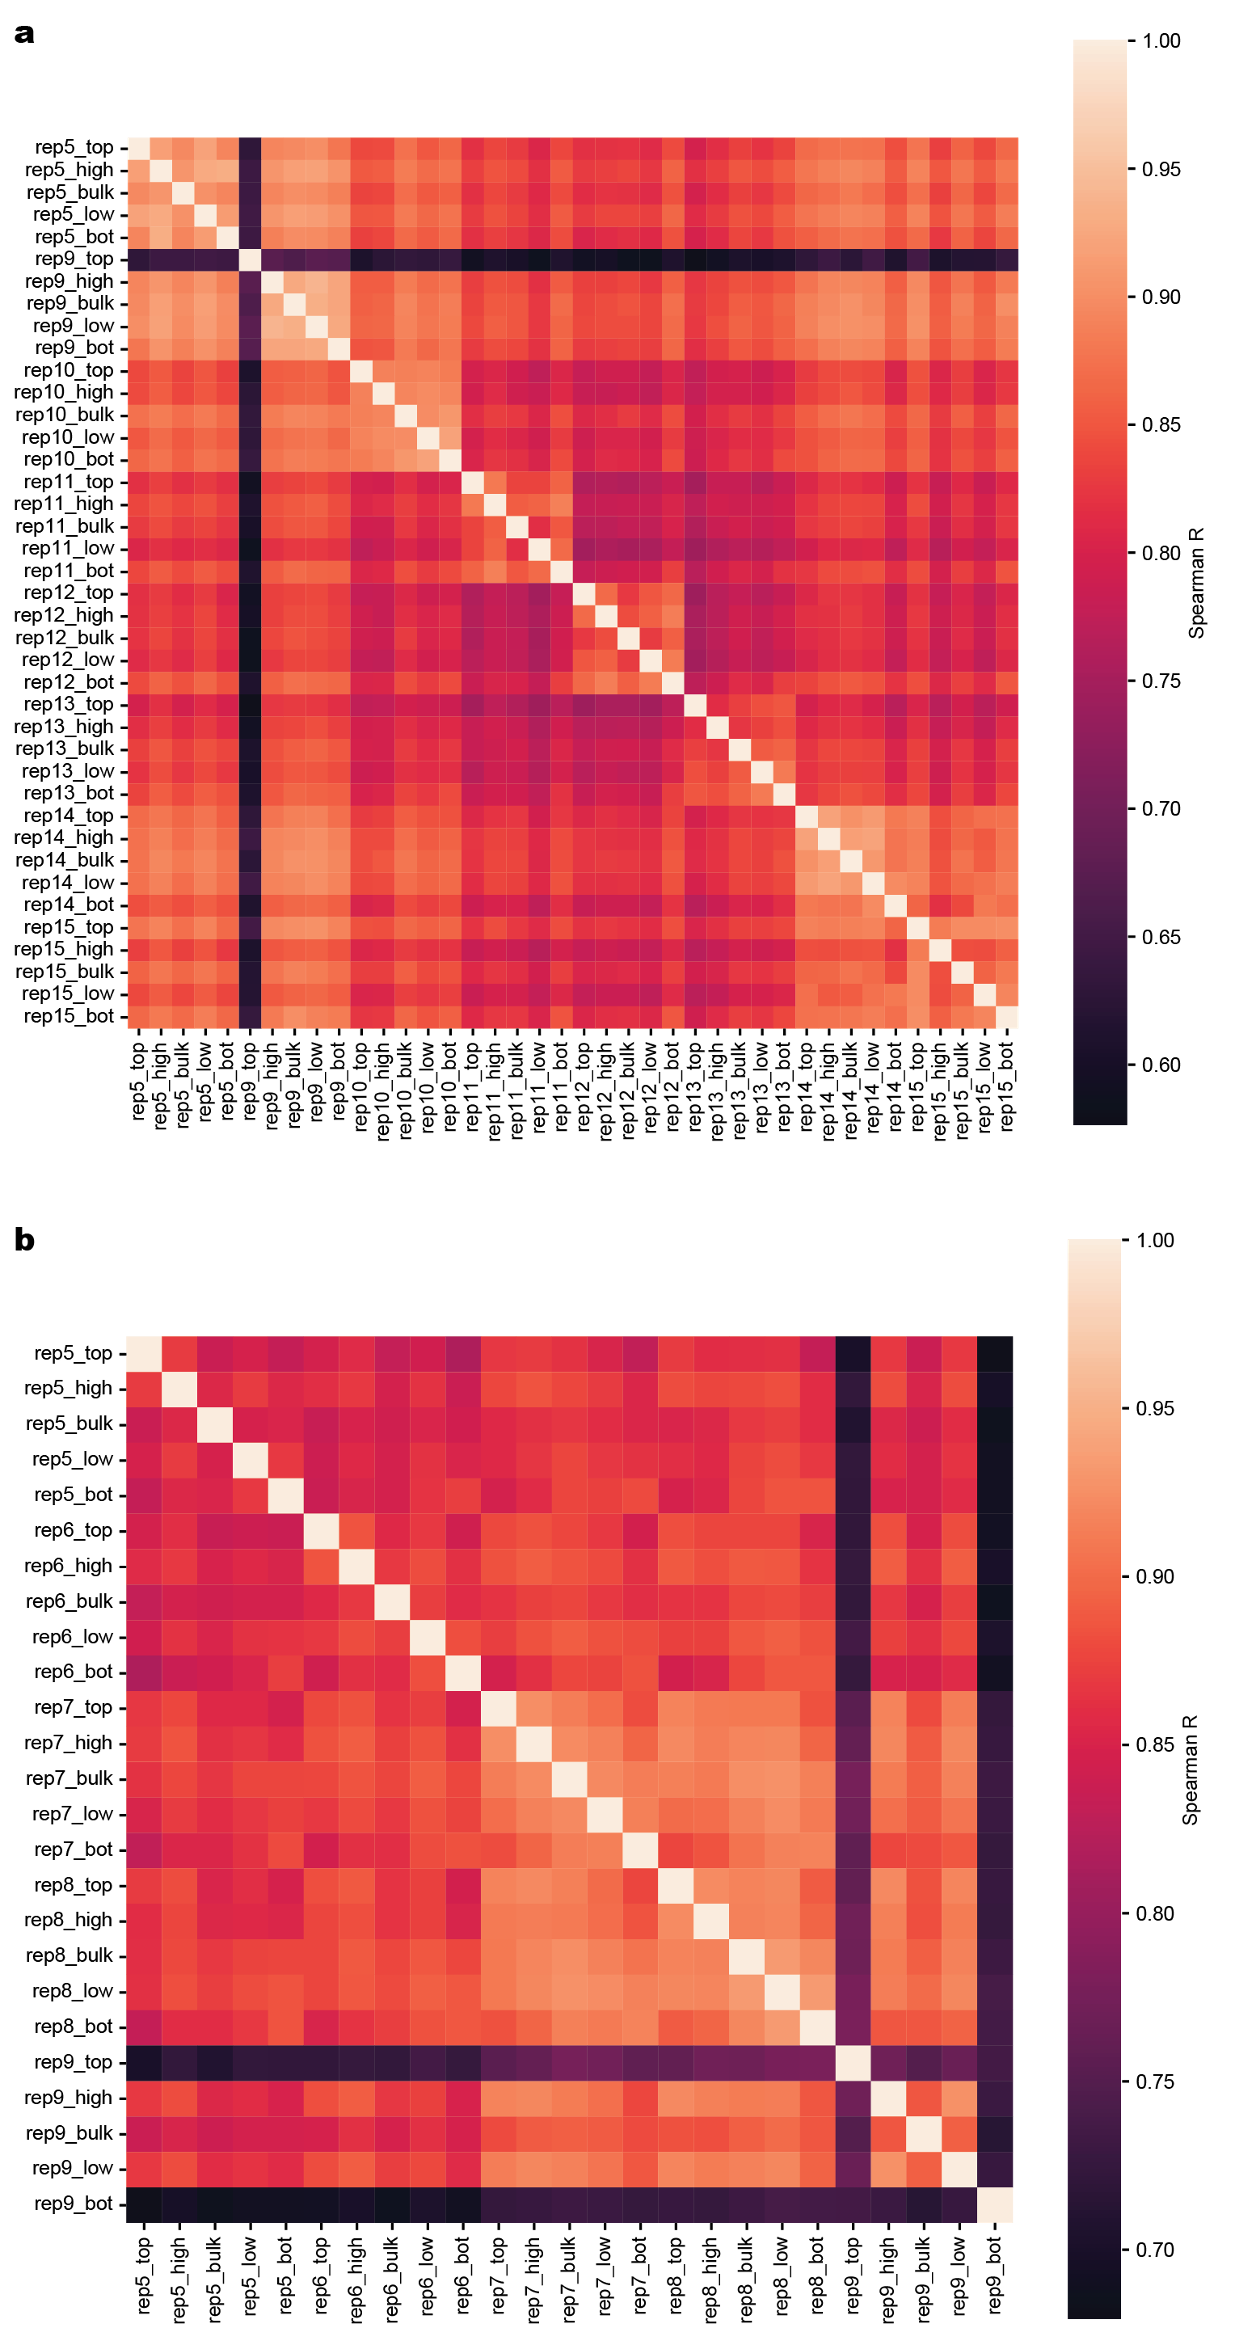
\includegraphics[scale=0.9]{figures/crisprbean4.png}
	\caption[Base editing screen read correlations]{\textbf{Base editing screen read correlations. } Spearman correlation coefficient of \textbf{(A)} gRNA counts of LDL-C GWAS library and \textbf{(B)} LDLR tiling library samples after filtering out for gRNAs with less than 10 read counts. Top; 80-100\%, high; 60-80\%, low; 20-40\%, bot: 0-20\% percentile LDL-C uptake. Rep; experimental replicate.}
	\label{fig:crisprbean4}
\end{figure} 
% -- Activity-normalized base editing screen analysis with BEAN
\subsection{Activity-normalized base editing screen analysis with BEAN}
We postulated that the gRNA editing outcomes provided by the reporter together with the accessibility of the target region could improve the quantification of variant phenotypic effects in our pooled BE screens. To do so, we developed a novel analysis method, BEAN (Base Editor screen analysis with Activity Normalization), to quantify the effect of each variant from gRNA abundance in sorted populations along with genotypic outcome information provided by reporter editing. BEAN assumes that the observed phenotypic distribution in a population of cells for each gRNA derives from a mixture of cells with unedited and edited alleles (\textbf{Fig. \ref{fig:crisprbean5}}). The proportion of cells carrying a given gRNA that possess a particular genotype is inferred based on the editing outcome observed in reporter as well as chromatin accessibility of the target locus using a Bayesian network. The distribution of cells with each gRNA prior to sorting is modeled as a Gaussian mixture for each underlying genotype produced by that gRNA. Because multiple gRNAs may induce the same genotypic outcome at different frequencies, BEAN uses this redundancy to build confidence in the predicted phenotypic impacts of a given genotype. As the output for each variant, BEAN provides its effect size i.e. the posterior mean phenotypic shift along with the corresponding $z$-score, and 95\% credible interval (CI). We also note that BEAN can be adapted to an arbitrary number and arrangement of sorting bins and other base editing enzymes including those with uncharacterized editing preferences, and can accommodate screens without reporter or accessibility information. 
\begin{figure}
	\centering
	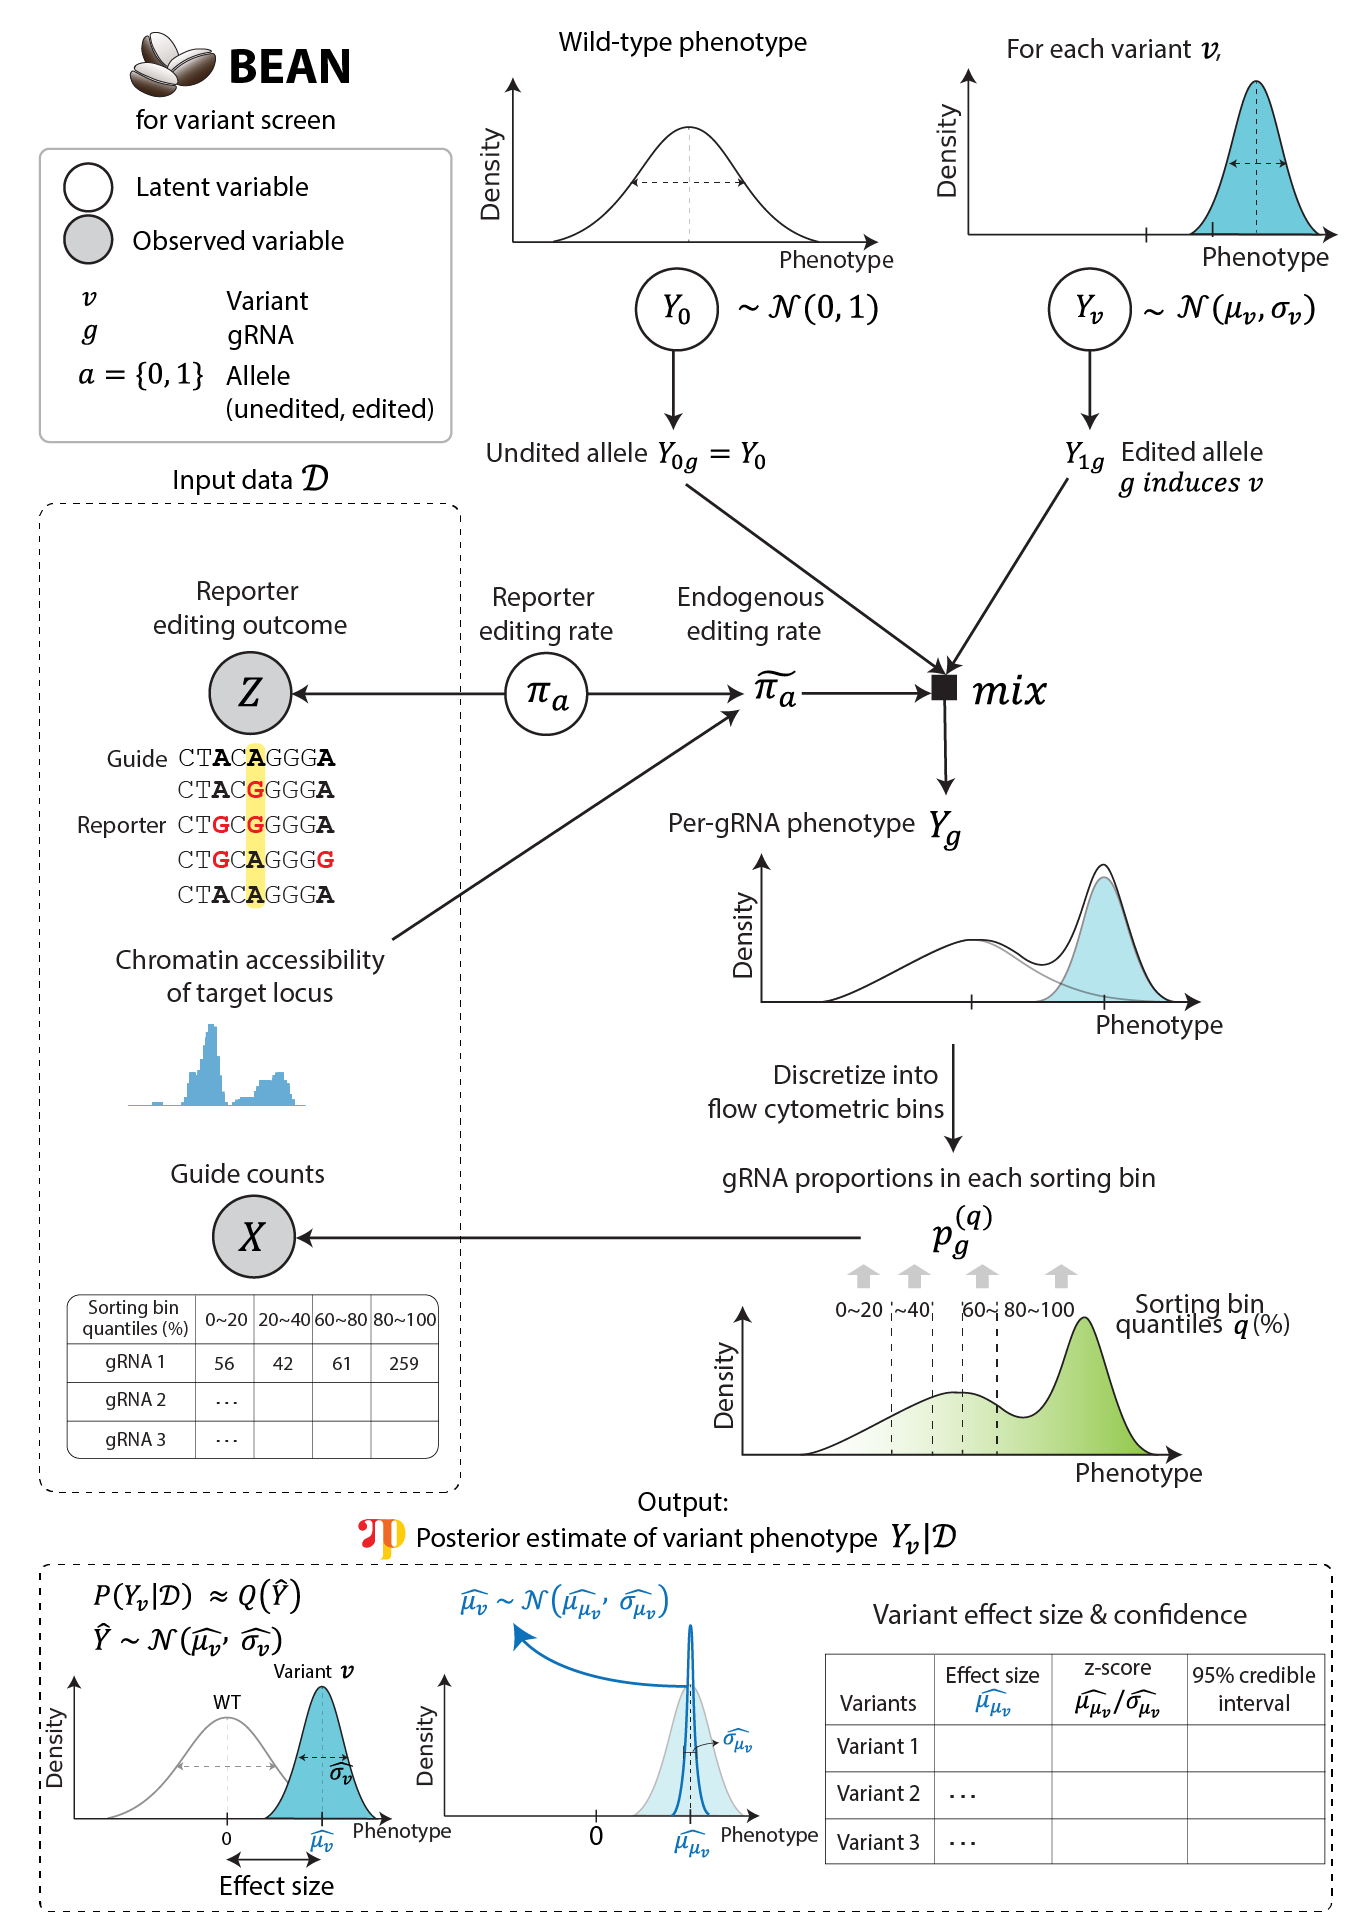
\includegraphics[width=\textwidth]{figures/crisprbean5.png}
	\caption[BEAN models variant effects from activity-normalized base editing screens]{\textbf{BEAN models variant effects from activity-normalized base editing screens. } Simplified schematic of BEAN Bayesian network that models input reporter editing outcomes and gRNA counts. The Bayesian network model recapitulates the data generation process starting from a variant-level phenotype Y$_{v}$ and models per-gRNA phenotypes as a Gaussian mixture distribution of edited and unedited (wild-type) allele phenotypes. The weights of the mixture components are modeled to generate reporter editing outcomes. gRNA abundance in each sorting bin is then calculated by discretizing the gRNA phenotype based on the experimental design into the phenotypic quantiles, and is modeled to generate the observed gRNA counts using an overdispersed multivariate count distribution (see Methods). BEAN outputs the parameters of the posterior distribution of mean phenotypic shift as Gaussian distribution with mean $\hat{\mu_{\mu}}$ (effect size), along with negative-control adjusted $z$-score  and credible interval (CI), where $\mathcal{D}$ is the input data.}
	\label{fig:crisprbean5}
\end{figure} 

BEAN only assumes population-level consistency between editing of the reporter and endogenous target site. We hypothesized that variation in editor expression or cellular state may lead certain cells to be more amenable to editing than others. In this scenario, “jackpot” cells would be more likely to have editing at both endogenous and reporter loci. To assess this possibility, we compared the enrichment of a gRNA in the highest vs. lowest sorted LDL uptake quantile bin with the difference in reporter editing observed in cells sorted into these bins, reasoning that endogenous editing should be highest in the cells sorted into the enriched bin. We indeed observed such correlation for LDLR and MYLIP splice-ablating gRNAs (Spearman $\rho$=0.32, \textbf{Fig. \ref{fig:crisprbean6}}), suggesting the existence of cell-level factors leading to “jackpot” cells with higher editing at both endogenous and reporter loci. However, the correlation between phenotypic and reporter editing enrichment was weaker when considering all positive control gRNAs (Spearman $\rho$=0.13). We thus concluded that incorporating the jackpot effect into BEAN would be unlikely to improve model performance.
\begin{figure}
	\centering
	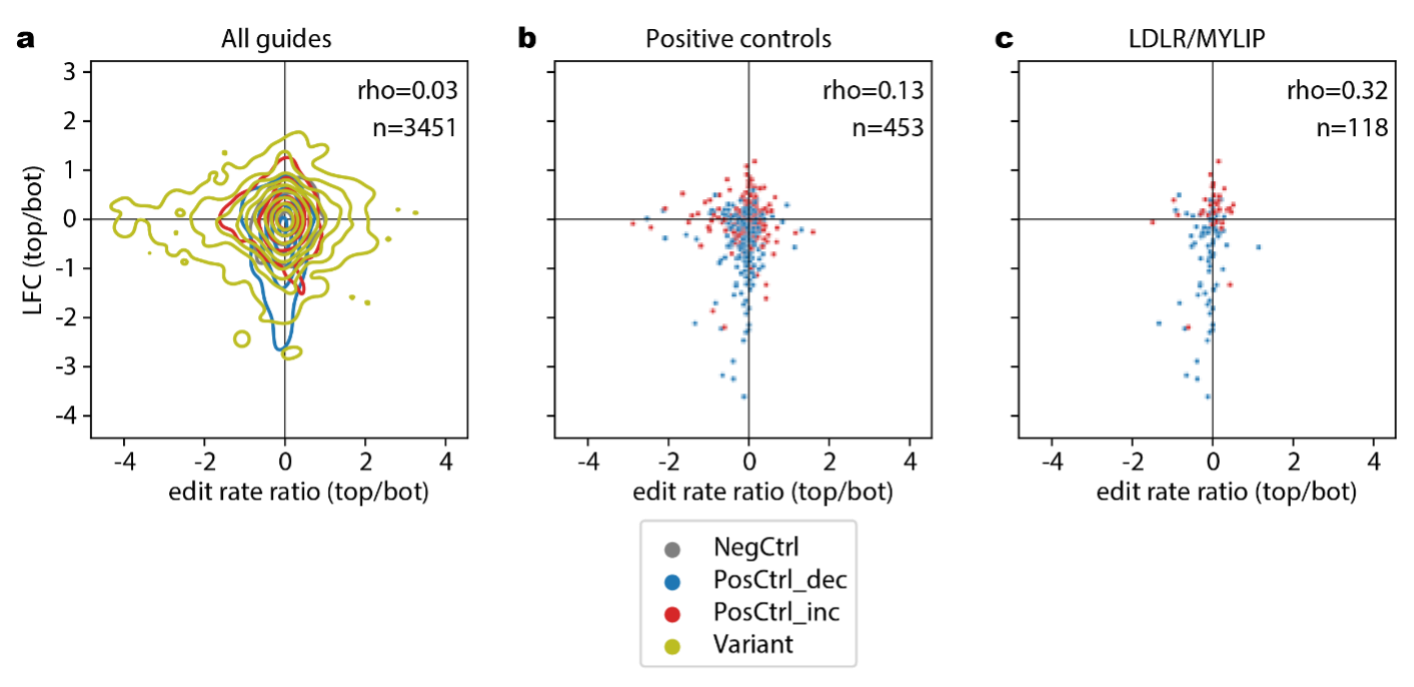
\includegraphics[width=\textwidth]{figures/crisprbean6.png}
	\caption[Jackpot analysis]{\textbf{Jackpot analysis. } Scatterplots of editing rate enrichment plotted against gRNA abundance enrichment of \textbf{(A)} all gRNAs, \textbf{(B)} positive control gRNAs, \textbf{(C)} strongest positive control gRNAs targeting LDLR or MYLIP splicing sites. Enrichment of both editing efficiencies and gRNA abundance is calculated as the log fold chance of the measures in the highest and lowest 20\% quantile bin. Spearman correlation coefficients are shown as rho. NegCtrl; negative control gRNAs, PosCtrl\_dec; positive control gRNAs that is expected to decrease LDL-C uptake, PosCtrl\_inc; positive control gRNAs that is expected to increase LDL-C uptake.}
	\label{fig:crisprbean6}
\end{figure} 
% -- BEAN identifies LDL uptake altering GWAS variants
\subsection{BEAN identifies LDL uptake altering GWAS variants}
We applied BEAN to the LDL-C GWAS library screen. From the reporter data, variant editing efficiency per gRNA is highly variable with average edit fraction of 34.0\%. Encouragingly, most target variants are edited at high efficiency by at least one of the five targeting gRNAs (median maximal editing of 60.4\%, \textbf{Fig. \ref{fig:crisprbean7}}). 
\begin{figure}
	\centering
	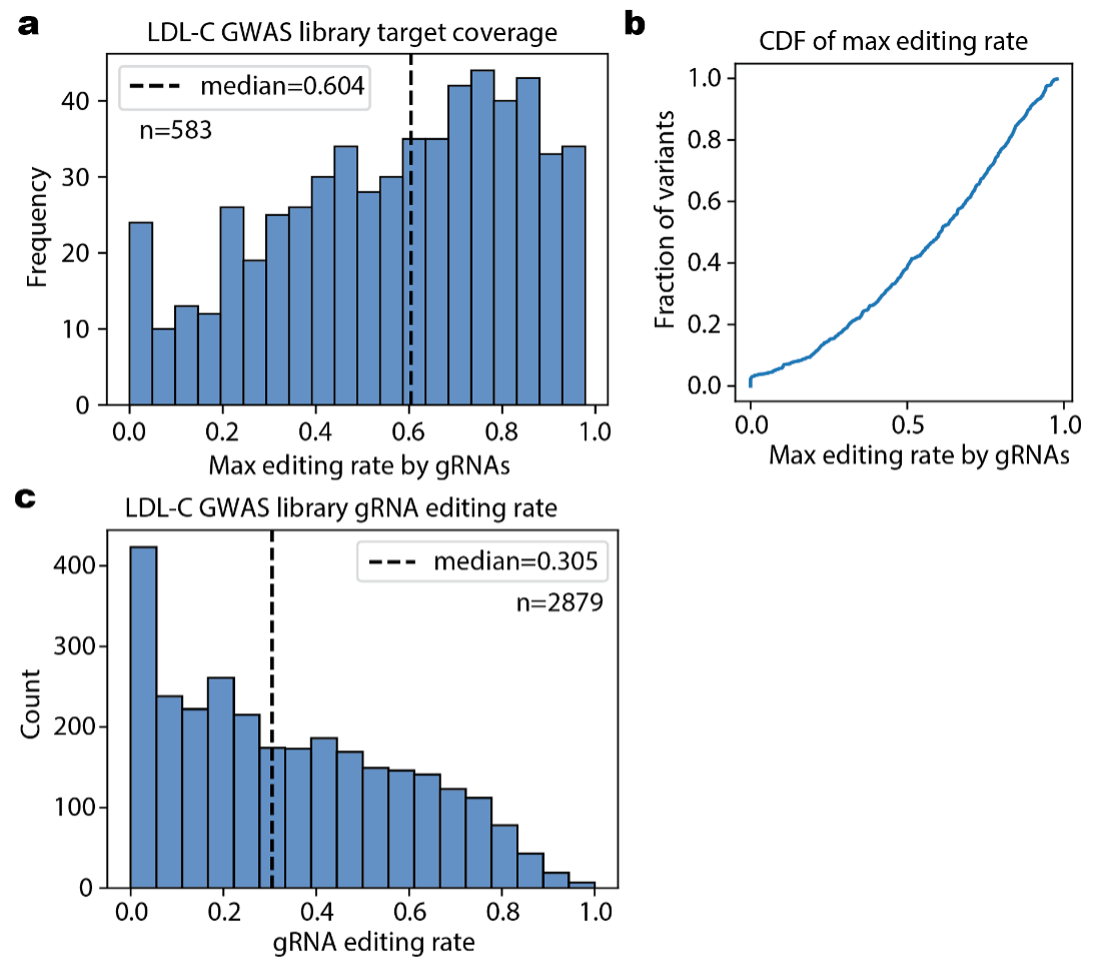
\includegraphics[width=\textwidth]{figures/crisprbean7.png}
	\caption[LDL-C GWAS variant editing coverage]{\textbf{LDL-C GWAS variant editing coverage.} \textbf{(A)} Histogram of per-target variant coverage calculated by the maximal editing rate of the variant by any gRNAs targeting the variant, where gRNA editing rates are calculated as the mean editing rate in bulk samples across replicates where more than 10 reads are observed. \textbf{(B)} Cumulative distribution function of the same distribution plotted in \textbf{(A)}. \textbf{(C)} Per-gRNA editing rate of the target variant in bulk samples across replicates where more than 10 reads are observed. }
	\label{fig:crisprbean7}
\end{figure} 
First, we compared the performance of BEAN and five published CRISPR screen analysis methods at distinguishing the effects of positive control splice-altering variants versus negative control non-targeting gRNAs \citep{huang2021identification, li2014mageck, li2015quality, jeong2019beta, daley2018crisphiermix}  \textbf{Fig. \ref{fig:crisprbean8}(A)}). To dissect the contributions of individual features to BEAN performance, we included two reduced versions of BEAN: one that considers reporter editing but not chromatin accessibility (BEAN-Reporter), and another that ignores the reporter, assuming uniform gRNA editing efficiency (BEAN-Uniform). BEAN outperforms other evaluated methods at this classification task (\textbf{Fig. \ref{fig:crisprbean8}(B)})), and this improved performance is accentuated when the data is subsampled for fewer replicates, demonstrating its ability to maintain robustness even with less data. Importantly, BEAN shows improved performance (mean AUPRC=0.90 across 15 2-replicate subsamples) over BEAN-Reporter (mean AUPRC=0.87), which in turn outperforms BEAN-Uniform (mean AUPRC=0.85), supporting the value of accurately modeling target site editing. Intriguingly, even BEAN-Uniform outperforms alternative approaches, likely due to more accurate modeling of sorting bins, suggesting the utility of BEAN in sorting screens without reporter.
\begin{figure}
	\centering
	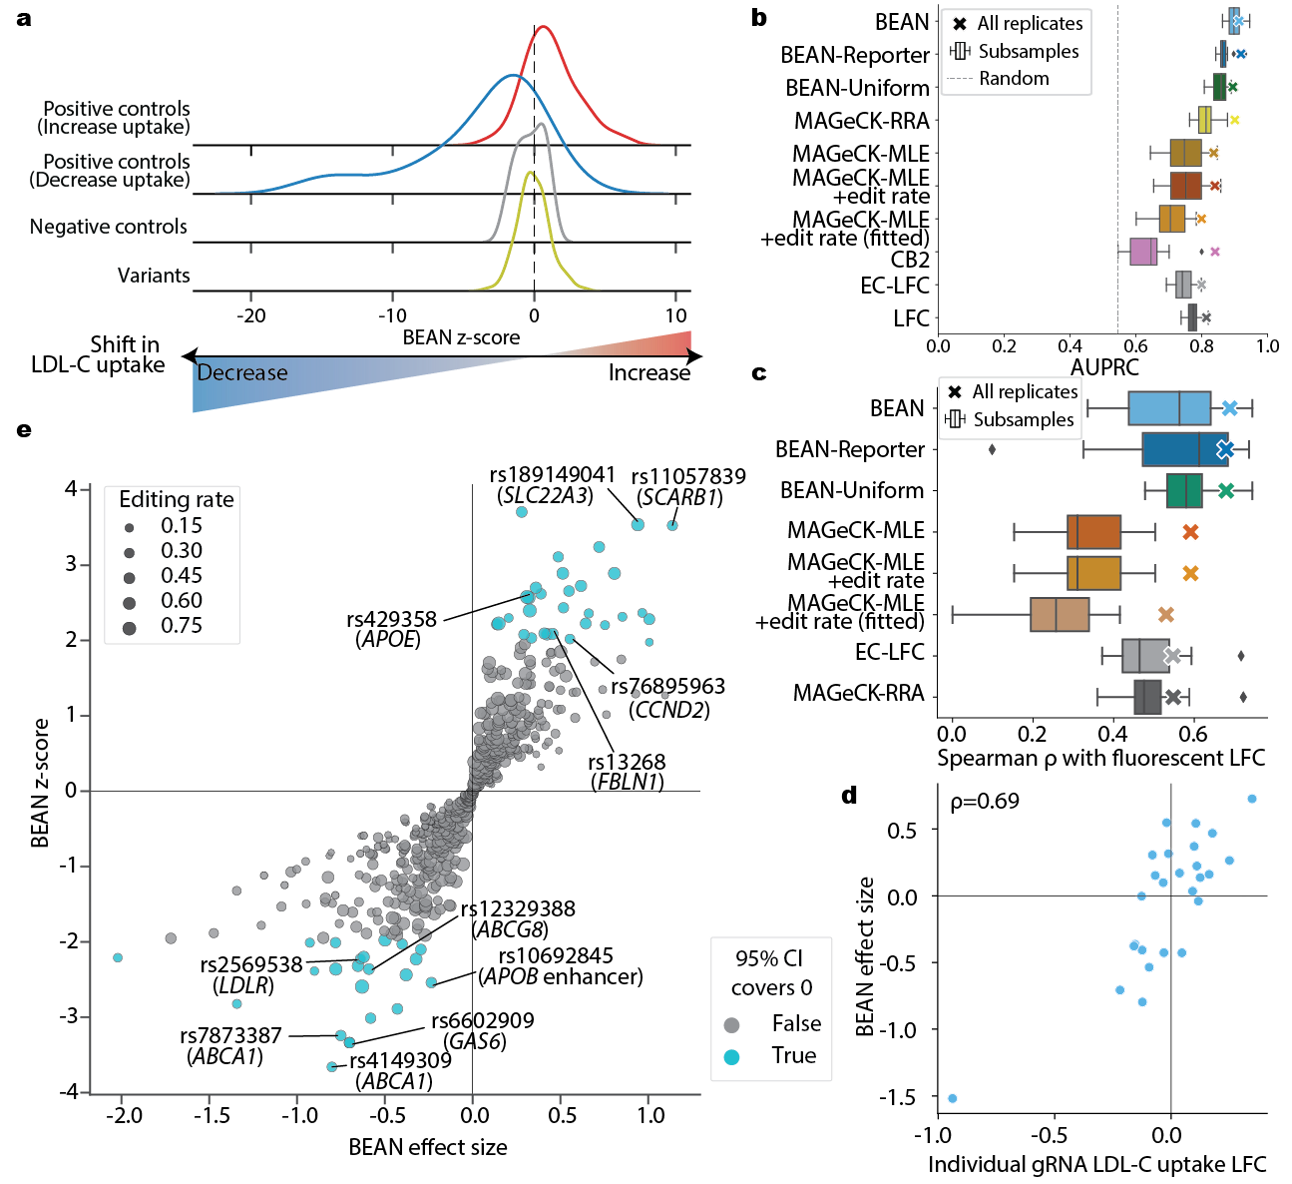
\includegraphics[width=\textwidth]{figures/crisprbean8.png}
	\caption[BEAN improves variant impact estimation from the LDL-C GWAS library screen]{\textbf{BEAN improves variant impact estimation from the LDL-C GWAS library screen.  (A)} Ridge plot of BEAN $z$-score distributions of positive controls, negative controls, and test variants. \textbf{(B)} AUPRC of classifying LDLR and MYLIP splicing variants vs.  negative controls. Metrics for all 5 replicates are shown as markers and metrics of 15 two-replicate subsamples among the 5 replicates are shown as box plots. \textbf{(C)} Spearman correlation coefficient between BEAN effect size and log fold change of LDL-C uptake following individual testing of 26 gRNAs. Metrics for all 5 replicates are shown as marker and metrics of 15 two-replicate subsamples among the 5 replicates are shown as box plots. \textbf{(D)} Scatterplot of BEAN effect size and log fold change of LDL-C uptake following individual testing of 26 gRNAs. Spearman correlation coefficient is denoted as $\rho$. \textbf{(E)} Scatterplot of variant effect size and significance estimated by BEAN. Labels show rsIDs of selected variants and dbSNP gene annotations and a manual annotation for APOB enhancer in the parenthesis.}
	\label{fig:crisprbean8}
\end{figure} 
Having demonstrated robust performance of BEAN, we evaluated our ability to characterize common variants that alter LDL-C uptake. We identified 54 variants that significantly alter LDL-C uptake (95\% CI does not contain 0). These variants include intronic variants in well-known LDL-C uptake mediators whose knockout altered LDL-C uptake in a recent genome-scale CRISPR screen37 such as ABCA1, LDLR, and SCARB1 (\textbf{Fig. \ref{fig:crisprbean8}(E)}). We additionally identified coding/intronic variants in APOE, CCND2, GAS6, and FBLN1 with strong genetic likelihood of causality (UKBB SUSIE fine-mapping PIP > 0.99 and/or the only variant in a fine-mapped credible set\citep{graham2021power}), indicating that the effect of these variants on serum LDL-C is at least partially mediated by LDL-C uptake. To validate the inferred effect sizes, we performed individual lentiviral ABE8e-SpRY transduction of HepG2 cells with gRNAs targeting 22 variants and 4 positive controls. We performed fluorescent LDL-C uptake profiling of each edited cell line mixed with an in-well control cell line in 6 biological replicates, allowing us to compare changes in LDL-C uptake with matched data from the screen. The individual LDL-C uptake log-fold-change (LFC) values showed strong correlation to the BEAN effect sizes ($\mu$, Spearman R=0.69, \textbf{Fig. \ref{fig:crisprbean8}(C)} and \textbf{D}), showing more robust correlation than BEAN-Uniform (R=0.68), log fold change based on MAGeCK-RRA (R=0.51), and regression coefficients $\beta$ of MAGeCK-MLE (R=0.61). These data demonstrate that BEAN enables accurate inference of variant effects on LDL-C uptake over a wide dynamic range.

To gain insight into a set of 20 variants for which the mechanism of LDL-C uptake alteration is less clear, we developed a pipeline to assess the cellular effects of variant installation (\textbf{Fig. \ref{fig:crisprbean9}(A)}). First, we asked which of these variants impact chromatin accessibility. We established an approach to perform pooled variant editing followed by ATAC-seq. High multiplicity of infection (MOI) lentiviral delivery of a pool of 20 ABE8e-SpRY gRNAs to HepG2 cells was followed by ATAC-seq and paired genomic DNA collection in three biological replicates in standard and serum-starved conditions. We performed multiplexed PCR enrichment of the regions surrounding each of the 20 edited variants followed by targeted amplicon sequencing by NGS. Differential representation of an alternate allele in ATAC-seq relative to gDNA sequencing implies differential accessibility of the alternate allele than the reference (\textbf{Fig. \ref{fig:crisprbean9}(B)}).
\begin{figure}
	\centering
	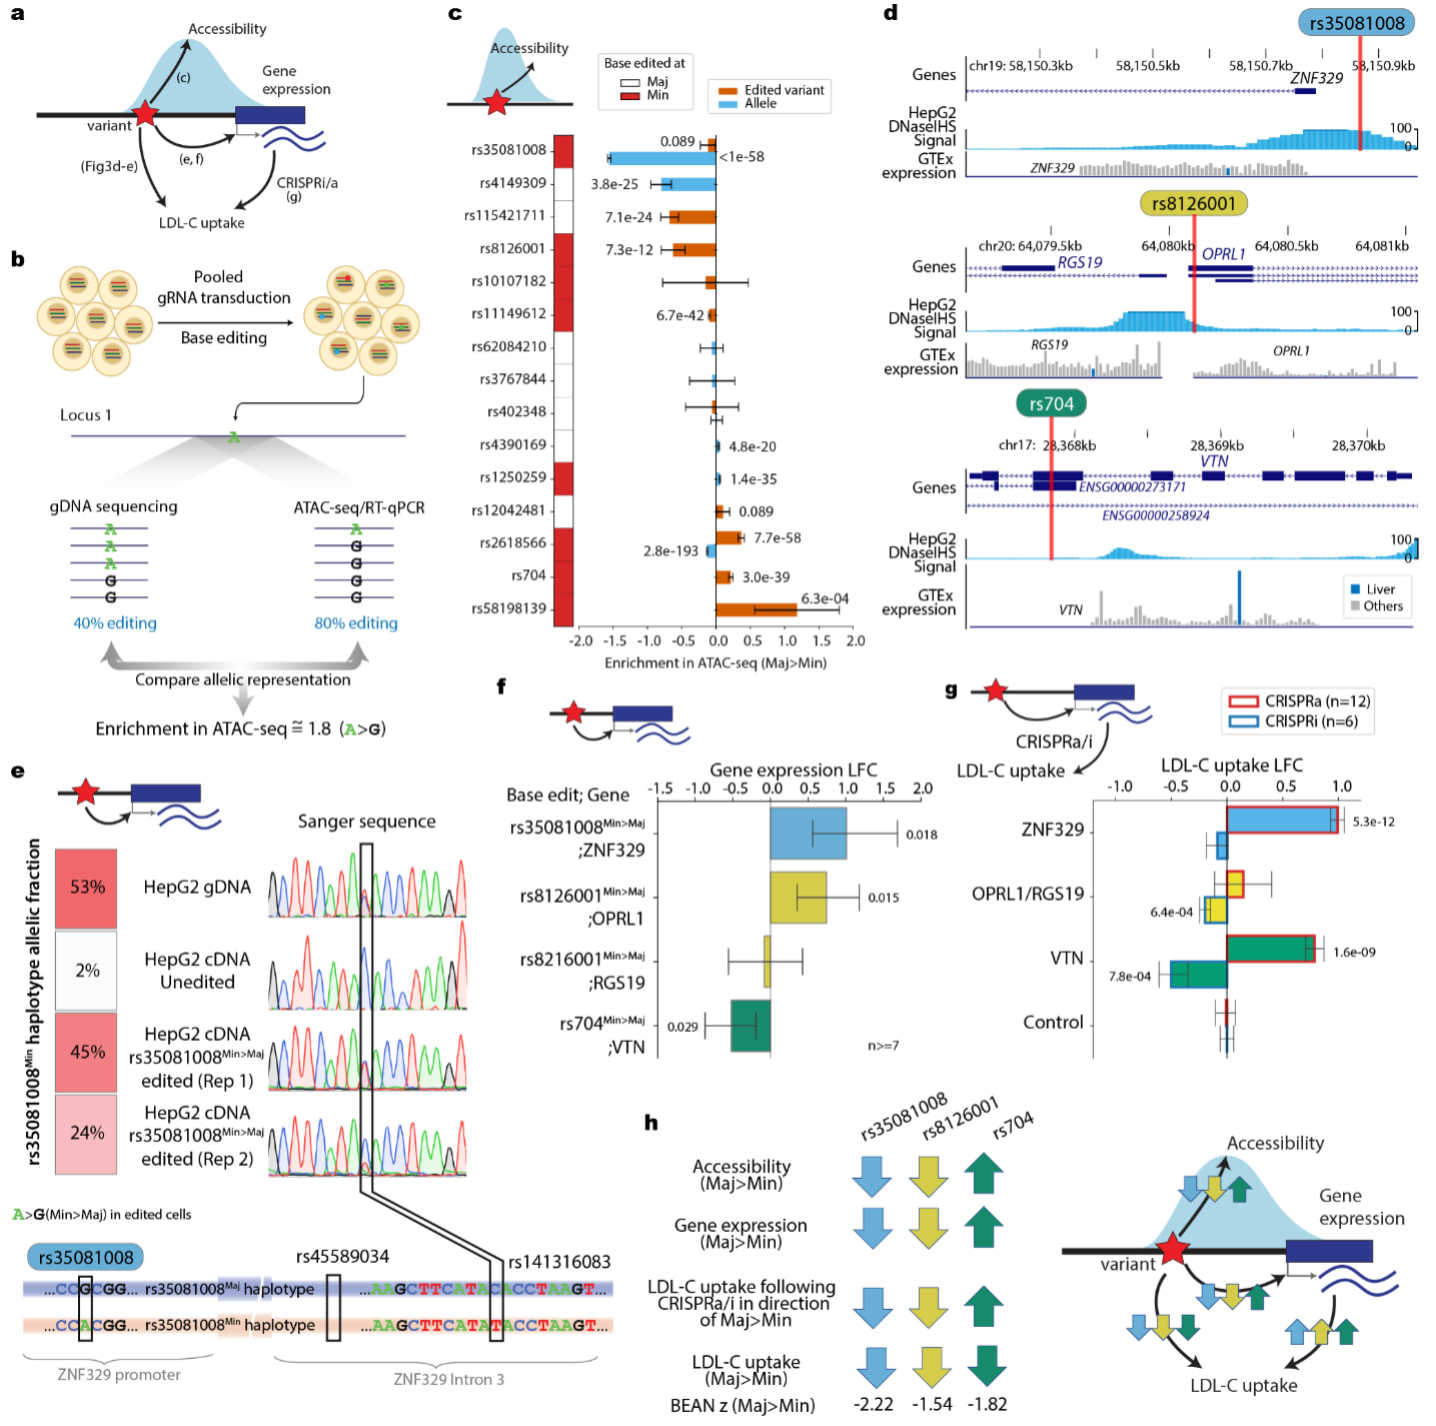
\includegraphics[width=\textwidth]{figures/crisprbean9.png}
	\caption[Functional characterization of LDL-C GWAS variants]{\textbf{Functional characterization of LDL-C GWAS variants.  (A)} Schematic of potential variant mechanisms and the figure panels showing data from each mechanistic experiment. \textbf{(B)} Schematic of pooled ATAC-seq analysis to identify variants impacting accessibility. Differential representation of allele in gDNA and ATAC-seq reflects differential accessibility induced by the base edit or heterozygous reference allele. \textbf{(C)} Change in ATAC-seq enrichment from the pooled ATAC-seq experiment. 95\% confidence intervals are shown as the error bars. “Edited variant” denotes the enrichment by base edit and “Allele” denotes the enrichment by either of the heterozygous alleles, when available, translated uniformly to major (Maj) to minor (Min) allele direction. Variants where the base edit is conducted from minor allele are denoted as red in the color bar. Family-wise error rate (FWER) with Benjamini-Hochberg multiple correction is shown for each enrichment value where FWER < 0.1. \textbf{(D)} Genomic tracks for three selected variants. DNaseIHS; DNase 1 Hypersensitivity. Multiple transcript variants of RGS19 and OPRL1 are shown in the middle panel. \textbf{(E)} Fraction of ZNF329 minor (Min) allele haplotype reads in gDNA and cDNA from untreated HepG2 and HepG2 with rs35081008Min>Maj base editing.  \textbf{(F)} Change in gene expression following base editing of three selected variants from minor (Min) to major (Maj) allele. P-values of the one sample Student’s t-test of LFC vs. mean of 0 that are smaller than 0.05 are shown above each bar. \textbf{(G)} Change in cellular LDL-C uptake following CRISPRa/i of proximal genes for three selected variants. P-values of the one sample Student’s t-test of LFC vs. mean of 0 that are smaller than 0.05 are shown above each bar. \textbf{(H)} Summary schematic of characterization results.}
	\label{fig:crisprbean9}
\end{figure} 
Eight of the 20 variants are heterozygous in HepG2, and thus we could assess whether these variants reside in chromatin accessibility quantitative trait loci (caQTL) \citep{degner2012dnase}, showing differential relative accessibility of the two haplotypes irrespective of base editing. We found five of these eight variants to be caQTLs (\textbf{Fig. \ref{fig:crisprbean9}(C)}). Two of these loci (rs35081008 and rs2618566) were also identified as caQTLs in a recent analysis of 20 human liver tissue samples \citep{currin2021genetic}. Importantly, caQTL analysis cannot address the causality of the evaluated variant due to the presence of linked variants which could contribute to the differential ATAC-seq signal. To assess whether individual variants alter chromatin accessibility, we evaluated whether base editing induces differential accessibility for any of the 20 tested variants. Technical issues including insufficient representation of the region, insufficient editing, and inability to phase heterozygous loci prevented assessment of five of the variants. Of the 15 remaining variants, eight significantly altered chromatin accessibility when edited (family-wise error rate 0.1, \textbf{Fig. \ref{fig:crisprbean9}(C)}). Four such variants (rs11149612, rs35081008, rs8126001, and rs2618566) were in loci identified as liver tissue caQTLs. Because base editing only alters a single variant in a locus, this analysis establishes at least partial causality to the tested variant. We performed deeper characterization of three variants whose editing alters both LDL-C uptake and chromatin accessibility. Rs704 is a missense coding variant in VTN and is the only variant in a fine-mapped credible set from LDL-C GWAS30, suggesting high likelihood of causality. The other two variants are in gene promoters—rs35081008 is in the ZNF329 promoter, and rs8126001 is in the shared OPRL1/RGS19 promoter \textbf{Fig. \ref{fig:crisprbean9}(D)}. Both variants have moderate probability of causality from GWAS evidence (SUSIE PIP=0.49 for rs35081008, PIP=0.25 for rs8126001), with the remaining probability in the rs35081008 locus deriving from a linked variant (rs34003091) 19-nt upstream in the ZNF329 promoter. None of the putative target genes has been previously found to alter LDL-C uptake, nor do they show significance in LDL-C burden analyses. To investigate how the prioritized variants might affect transcription factors (TF) binding sites and thereby regulate proximal genes involved in LDL-C uptake, we adapted the MotifRaptor pipeline \citep{yao2021motif}. For each variant, we retrieved genomic sequences spanning 61 bp centered around the SNP location, using the hg38 genome assembly as a reference. Each sequence was mutated by substituting the major allele with the minor allele at the SNP position, yielding both a reference and an alternative sequence for each variant. Subsequently, to evaluate the potential for transcription factor (TF) binding, we employed all the human TF position weight matrices (PWMs) from the CIS-BP database \citep{weirauch2014determination} to scan each pair of reference and alternative sequences. This motif scanning generated binding scores at each sequence position, serving as predictive indicators of TF binding potential. 
We then compared these scores for each TF across the reference and alternative alleles within every sequence pair. This comparative step is crucial for determining a variant's impact on TF binding. Specifically, higher binding scores for the alternative sequence indicate an increase in TF binding potential, while lower scores suggest a decrease. To quantify these changes, we calculated a 'disruption score' as follows: 
\[
\text{disruption} = \textrm{score($s_{alt}$)}- \textrm{score($s_{ref}$)}
\]
This score helps capture the directional change each variant induces, where a negative value signifies reduced TF binding potential and a positive value indicates an increase. For rs8126001, our approach prioritized two zinc finger TFs, ZNF333 and ZNF770 with enhanced binding site sequences due to the heterozygous minor allele in HepG2 cells (\textbf{Fig. \ref{fig:crisprbean10}}). HepG2 ChIP-seq data59 further support the binding of these TFs at this locus, although the variant lies at the edge of the peaks (\textbf{Fig. \ref{fig:crisprbean11}}). While definitive conclusions about these factors will require further experimental validation, our observations align with previous research \citep{farh2015genetic} suggesting that only a minority of causal variants directly alter canonical TF binding sequences and instead affect non-canonical sequences. 
\begin{figure}
	\centering
	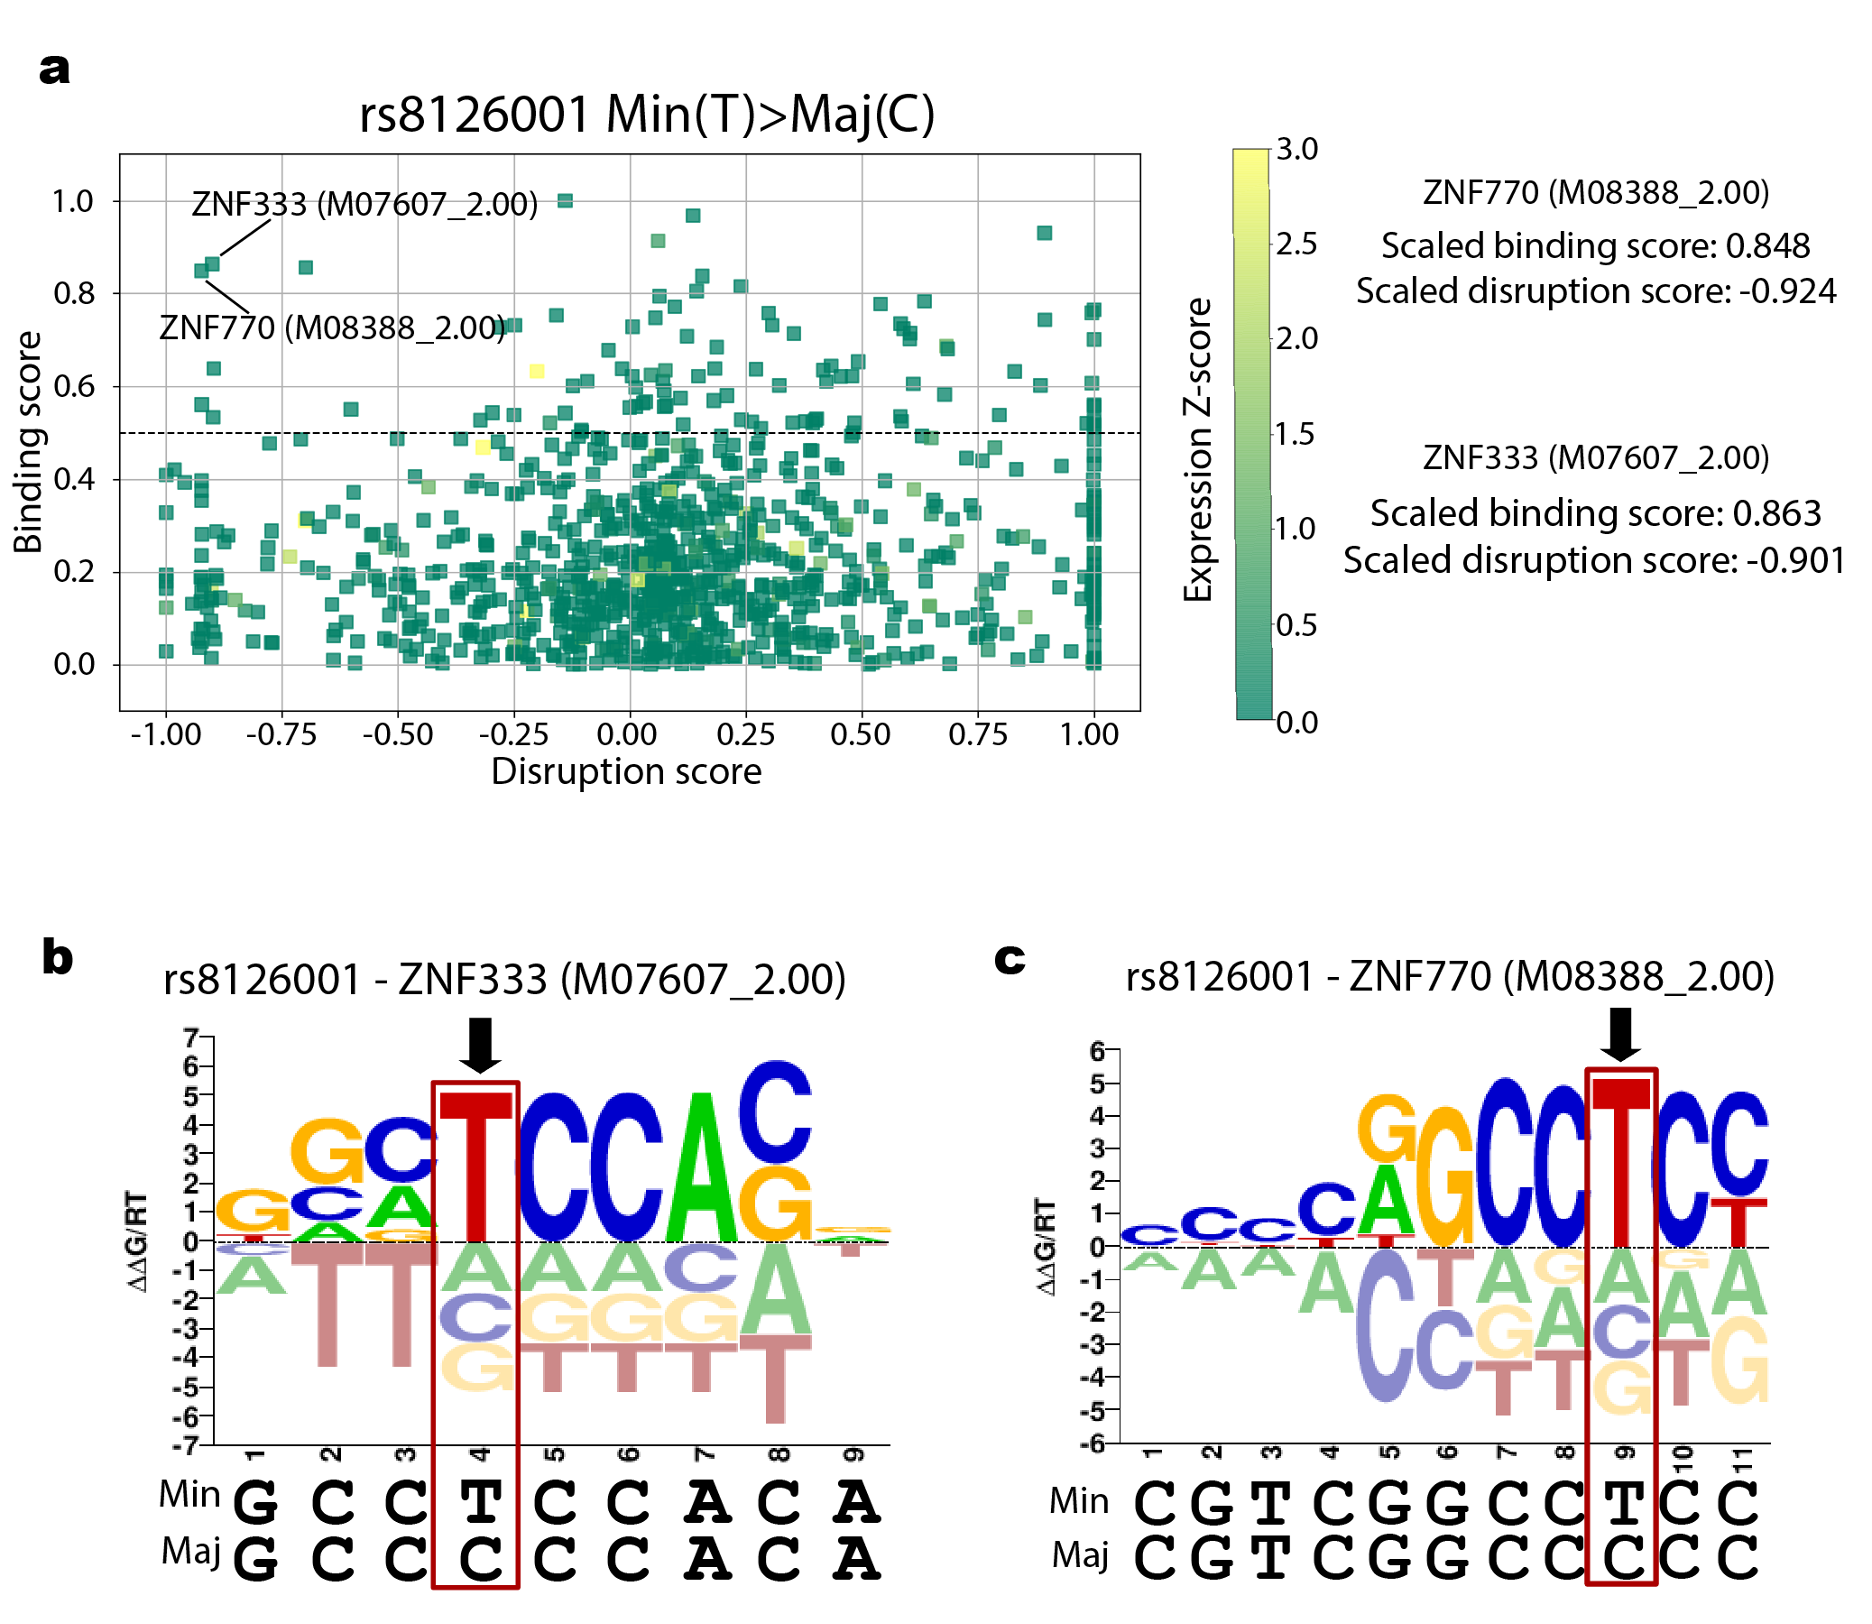
\includegraphics[width=\textwidth]{figures/crisprbean10.png}
	\caption[MotifRaptor analysis of candidate variant transcription factor binding disruption]{\textbf{MotifRaptor analysis of candidate variant transcription factor binding disruption.  (A)} Disruption plotted against binding score of motifs of rs8126001 minor allele transition to major. \textbf{(B-C)} Identified ZNF333 and ZNF770 motif aligned with rs8126001 loci with minor and major alleles.}
	\label{fig:crisprbean10}
\end{figure} 
\begin{figure}
	\centering
	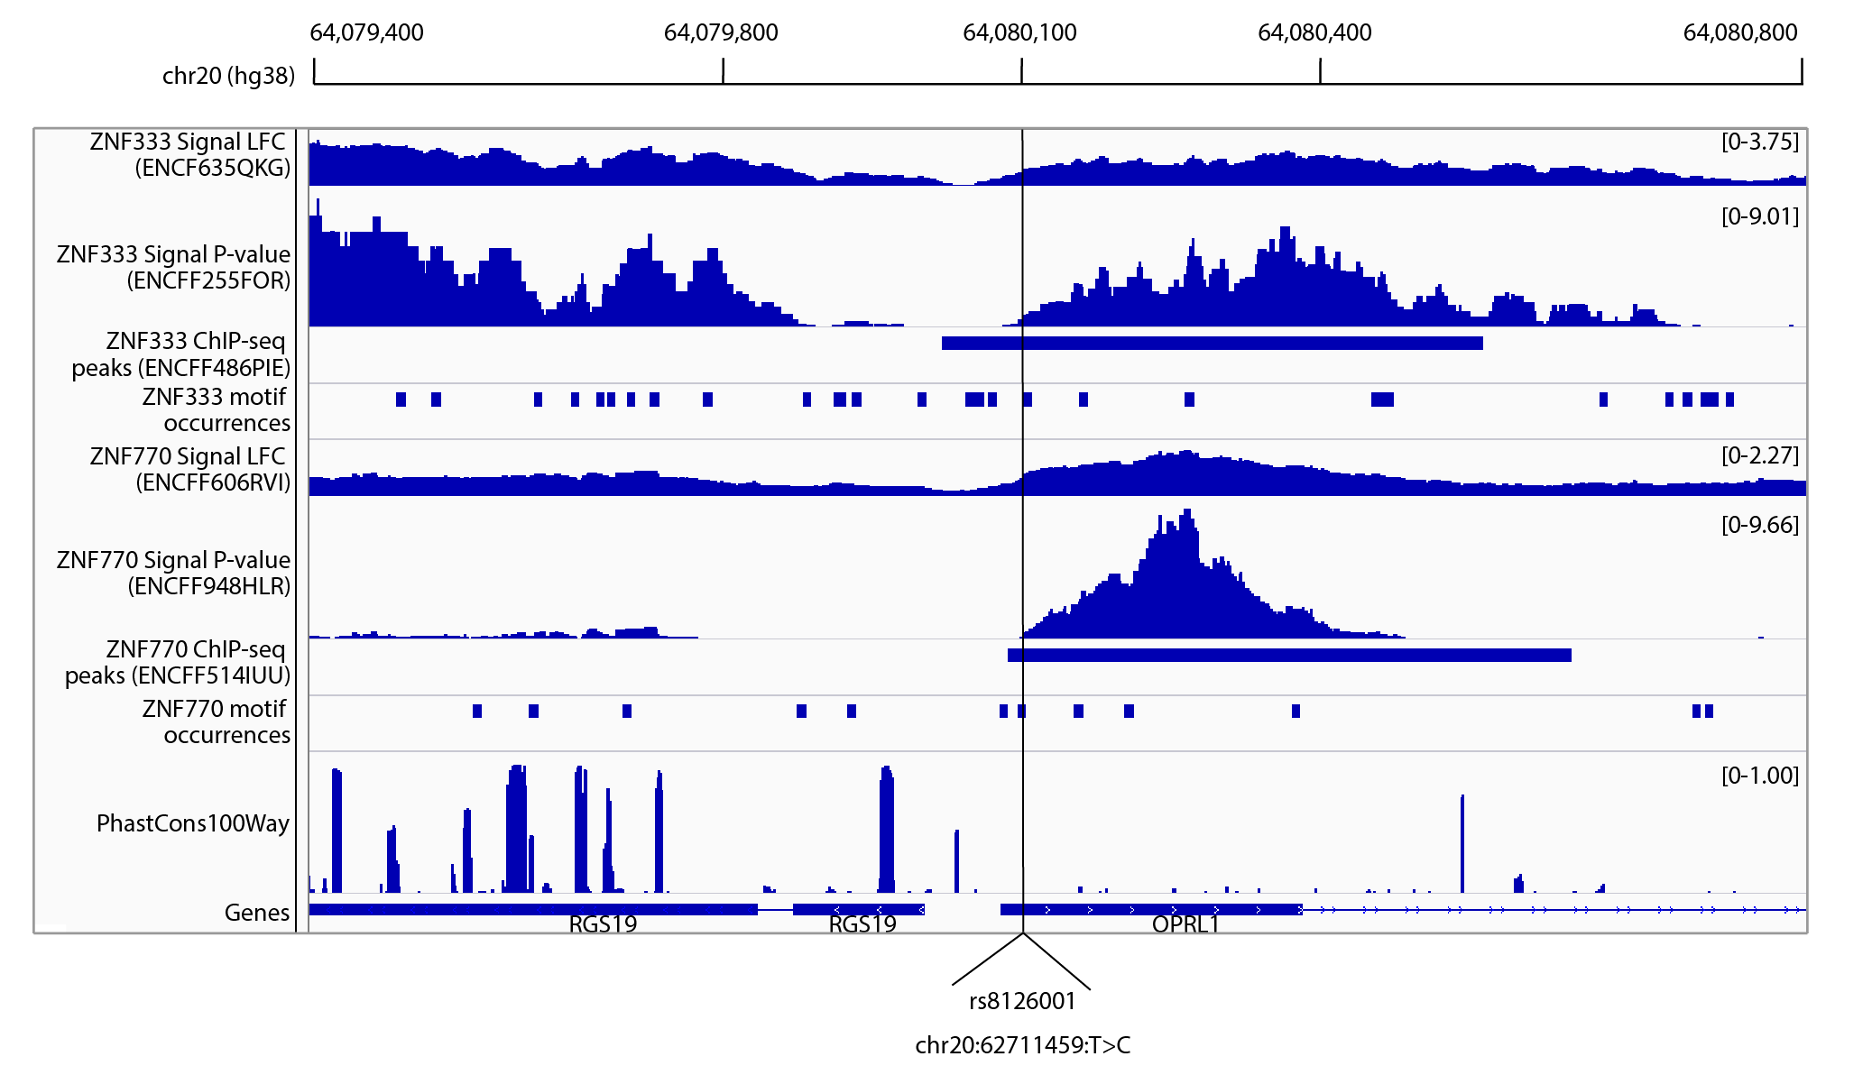
\includegraphics[width=\textwidth]{figures/crisprbean11.png}
	\caption[ChIP-seq signal LFC, signal P-values, peaks and motif occurrences of ZNF333 and ZNF770 around rs8126001]{\textbf{ChIP-seq signal LFC, signal P-values, peaks and motif occurrences of ZNF333 and ZNF770 around rs8126001.} PhastCons100way conservation scores and gene annotations are  displayed together. ENCODE accessions are shown in the parenthesis. }
	\label{fig:crisprbean11}
\end{figure} 
We confirmed through RT-qPCR analysis that editing the minor to major alleles of rs35081008 and rs8126001 leads to increased expression of ZNF329 and OPRL1 respectively (\textbf{Fig. \ref{fig:crisprbean9}(F)}), which is consistent with the increased chromatin accessibility induced by these edits. rs35081008 is heterozygous in HepG2, and we used two linked ZNF329 intronic variants to assess allele-specific expression. In wild-type HepG2, only 2\% of ZNF329 transcripts derive from the minor allele haplotype (\textbf{Fig. \ref{fig:crisprbean9}(E)}), consistent with the diminished chromatin accessibility of this allele (\textbf{Fig. \ref{fig:crisprbean9}(C)}) and the status of rs35081008 as a liver eQTL. Editing rs35081008 from minor to major allele restores expression of this haplotype to 35\% of total transcripts (\textbf{Fig. \ref{fig:crisprbean9}(E)}), providing further evidence that rs35081008Maj results in increased expression of ZNF329.We then performed CRISPRa and CRISPRi targeting to assess whether altered expression of the four candidate target genes alters LDL-C uptake. CRISPRa induction of VTN and ZNF329 significantly increased LDL-C uptake, and CRISPRi repression of VTN and OPRL1/RGS19 reduced LDL-C uptake (\textbf{Fig. \ref{fig:crisprbean9}(G)}). In our base editing experiments, rs704Min shows decreased LDL-C uptake, so we surmise that this allele must have decreased expression or function, given that decreased VTN expression decreases LDL-C uptake (\textbf{Fig. \ref{fig:crisprbean9}(H)}). Prior biochemical characterization has shown decreased cellular binding capacity of rs704Min , suggesting a possible mechanistic explanation. Our data are consistent with rs35081008Min decreasing ZNF329 expression, which in turn decreases LDL-C uptake. Finally, our data are most consistent with rs8126001Min decreasing OPRL1 expression, which leads to decreased LDL-C uptake. This observation aligns with the higher predictive binding affinity of ZNF333, a transcriptional repressor \citep{jing2004identification, witzgall1994kruppel}, with rs8126001Min and the potential disruption of its binding with rs8126001Maj. In summary, through accurately quantifying impacts of disease-associated variants on LDL-C uptake, BEAN reveals genetic mechanisms underlying control of LDL-C levels.
% -- Saturation LDLR coding sequence tiling screening enables quantitative assessment of rare variant deleteriousness 
\subsection{Saturation LDLR coding sequence tiling screening enables quantitative assessment of rare variant deleteriousness }
We next adapted BEAN to the LDLR tiling library, enhancing the model to specifically assess the contributions of individual amino acid mutations rather than SNVs, by enabling a more comprehensive understanding of coding region alterations. Previous coding sequence base editing analyses have assumed that all editable bases within a window are edited, which leads to erroneous amino acid mutation assignments, or have analyzed gRNA-level signal only \citep{martin2023massively}. We aimed to exploit the combination of dense tiling afforded by ABE8e-SpRY and reporter editing outcomes to model the effects of coding variants more accurately. The LDLR tiling screen showed high coverage of edited nucleotides and amino acids (92\% of targetable nucleotides and 74\% of the 860 LDLR amino acids in the LDLR coding sequence were edited at $>$10\% frequency by at least one gRNA in the reporter,. A total of 2,182 distinct variants were assessed, of which 874 are missense coding variants. Each gRNA produced an average of 2.6 distinct alleles, and each variant was covered by 5.8 gRNAs on average. Thus, ABE8e-SpRY tiling of LDLR resulted in a rich dataset of coding variants for the evaluation of their phenotypic impacts.
\begin{figure}
	\centering
	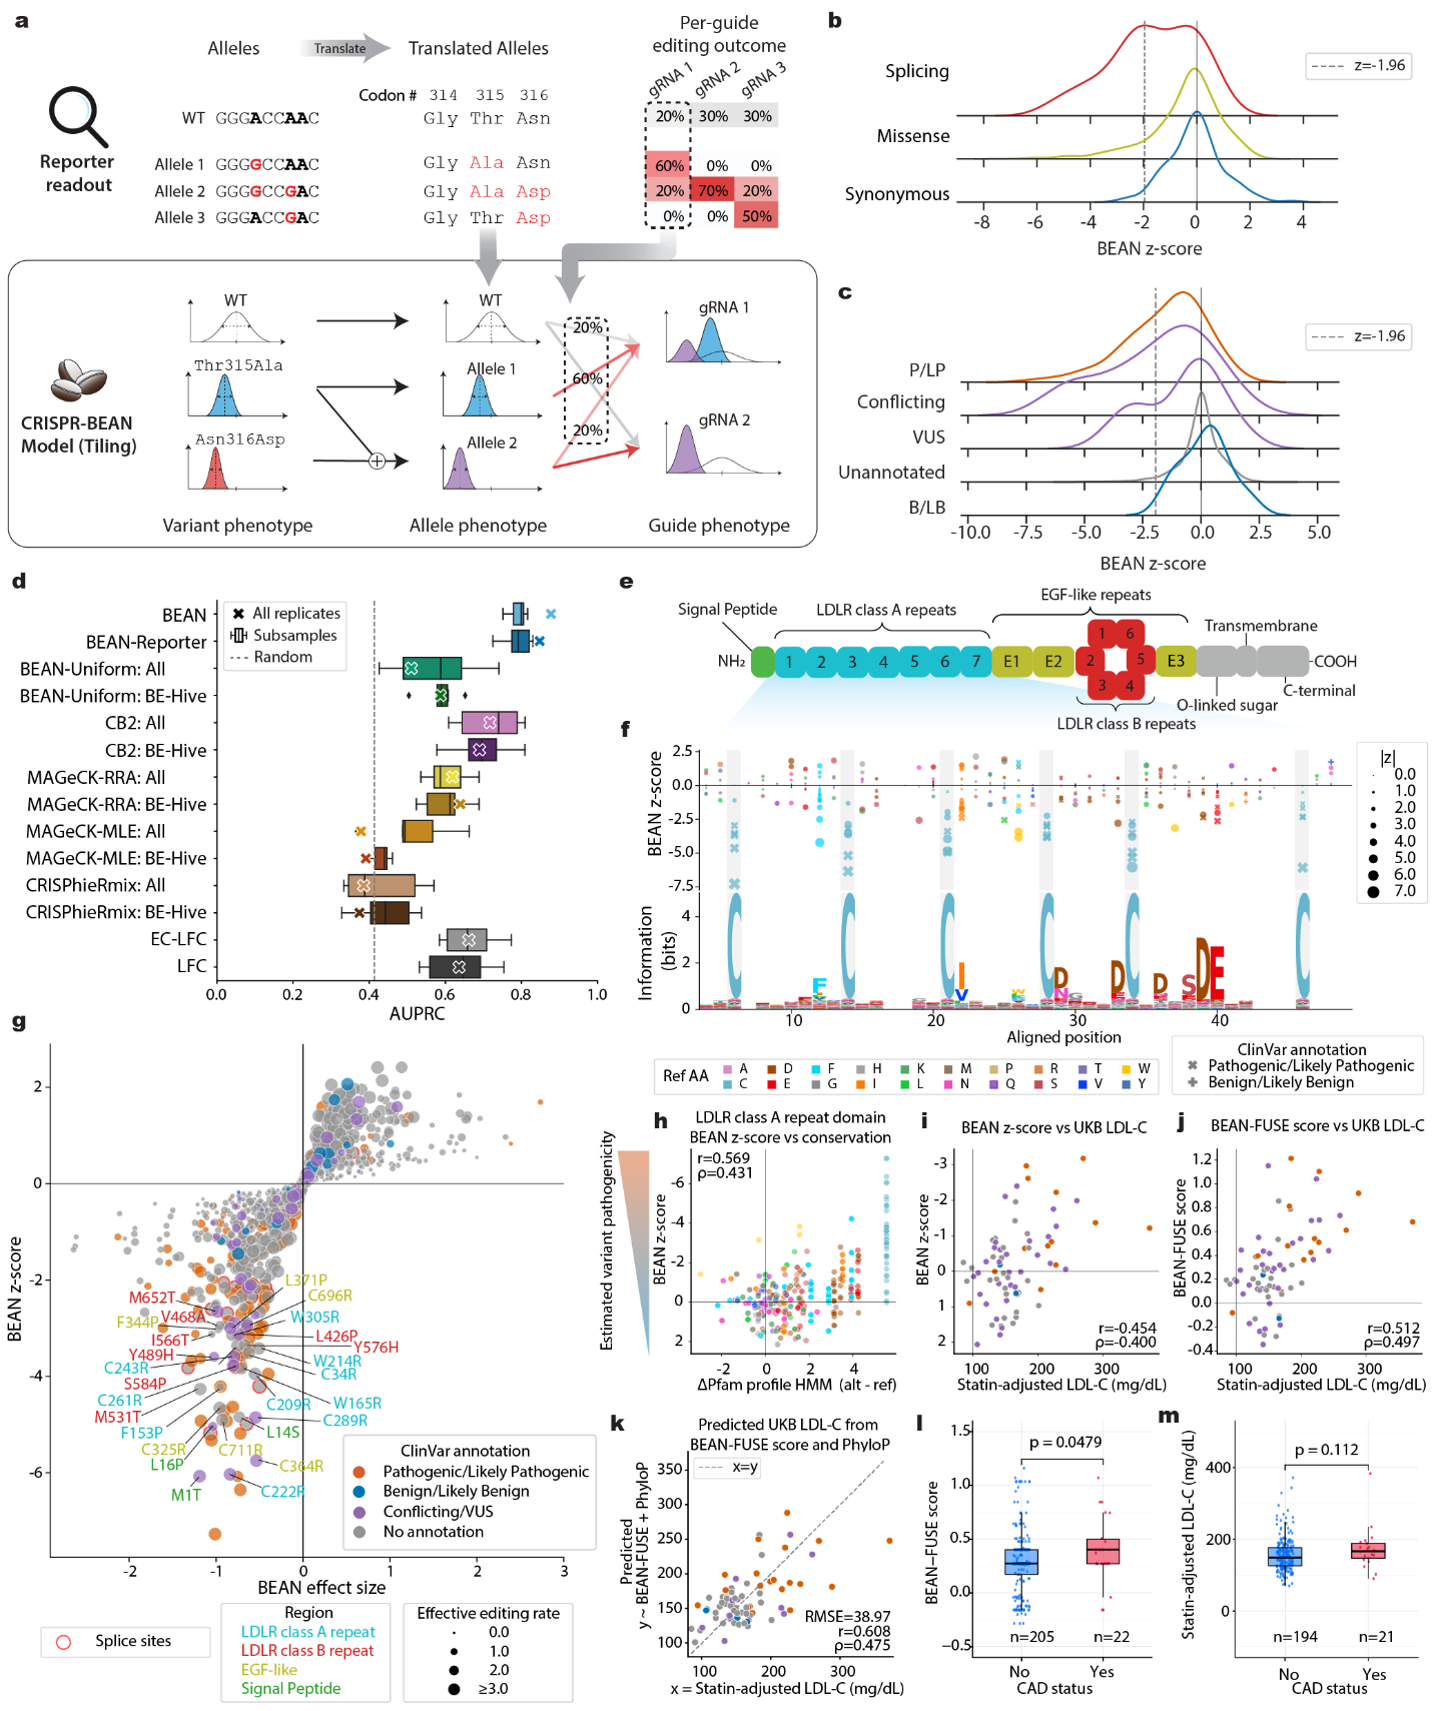
\includegraphics[width=\textwidth]{figures/crisprbean12.png}
	\caption[Dissection of LDLR variant effects through BEAN modeling of a saturation tiled base editing screen]{\textbf{Dissection of LDLR variant effects through BEAN modeling of a saturation tiled base editing screen. (A)} BEAN model for coding sequence tiling screens. Reporter editing efficiencies are calculated at the amino acid-level when the edited nucleotides are in coding region. Phenotypes of gRNAs with multi-allelic outcomes are modeled as the Gaussian mixture of allelic phenotypes. If an allele consists of more than one variant, the phenotype of the allele is modeled as the sum of the component variants. A Bayesian network is used to model variant-level phenotypes, sharing phenotypic information from all available gRNAs. \textbf{(B)} Ridge plot of BEAN z-score distributions of positive controls, negative controls, and variants. \textbf{(C)} Ridge plot of BEAN z-score distributions of Clinvar variants annotated as pathogenic/likely pathogenic (P/LP), benign/likely benign  (B/LB), conflicting interpretation of pathogenicity (conflicting), and Uncertain significance (VUS), and unannotated variants. \textbf{(D)} AUPRC of classifying ClinVar pathogenic/likely pathogenic vs. benign/likely benign variants. The marker shows the metrics of each method run on 4 replicates with no failing samples. Boxplot shows the metrics of 6 2-replicate combinations of the 4 replicates. \textbf{(E)} LDLR domain structure adopted from Oommen et al71. \textbf{(F)}BEAN $z$-scores for variants in the 7 LDLR class A repeat domains aligned with the Pfam profile HMM logo. Highly conserved cysteines are highlighted in grey. \textbf{(G)} Scatterplot of estimated variant effect sizes and z-scores. Labels of selected deleterious variants without ClinVar pathogenic/likely pathogenic annotations are shown. \textbf{(H)} Scatterplot of LDLR class A repeat missense variant BEAN $z$-scores and $\Delta$Pfam profile HMM scores. Higher $\Delta$Pfam scores correspond to substitution from highly conserved to rarely observed amino acids. \textbf{(I)} Comparison of mean statin-adjusted LDL-C level and BEAN z-score for variants observed in UKB and base editing. \textbf{(J)} Comparison of mean statin-adjusted LDL-C level and BEAN-FUSE scores for variants observed in UKB and base editing. \textbf{(K)} LDL-C levels of observed missense variants predicted by a regression model using BEAN-FUSE and PhyloP scores with 10-fold cross validation, compared with mean statin-adjusted LDL-C level in UKB. \textbf{(L)} Boxplots of BEAN-FUSE functional scores for UKB individuals with variants observed in our base editing screen with or without CAD. \textbf{(M)} Boxplots of statin-adjusted LDL-C levels of UKB invididuals with variants observed in our base editing screen with or without CAD. $P$-value of two-sided Wilcoxon rank-sum test is denoted. $r$; Pearson correlation coefficient, $\rho$; Spearman correlation coefficient}
	\label{fig:crisprbean12}
\end{figure} 
As opposed to the LDL-C GWAS analysis in which each gRNA was evaluated based on its editing frequency at a single target position, we adapted BEAN to account for multi-allelic outcomes. First, BEAN translates the edited alleles, i.e., aggregates nucleotide-level allele counts that leads to the identical amino acid transition into a single amino-acid level allele counts, while preserving nucleotide transition in non-coding regions. BEAN then filters for the translated alleles that are robustly observed for each gRNA (\textbf{Fig. \ref{fig:crisprbean12}(A)}). BEAN uses a Bayesian network to combine phenotypic information from all the gRNAs that produce a given allele. Importantly, the phenotype attributed to each gRNA is modeled as a mixture distribution of the alleles it generates, with the contribution of each allele weighted by its corresponding editing frequency.BEAN assigned significant z-scores ($<$-1.96, equivalent to 95\% credible interval not covering 0) to 145 among 2,182 variants assessed from the LDLR tiling library, 131 of which decrease LDL-C uptake. 47 variants that significantly decrease LDL-C uptake are annotated in ClinVar as pathogenic/likely pathogenic, while 17 are ClinVar VUS/conflicting variants and none are ClinVar benign/likely benign \textbf{Fig. \ref{fig:crisprbean12}(G)}), indicating that BEAN can reliably predict the pathogenicity for variants without a pathogenic or benign classification \textbf{Fig. \ref{fig:crisprbean12}(B)} and \textbf{(C)}). We compared the performance of BEAN at distinguishing ClinVar-annotated pathogenic from benign/likely benign LDLR variants to other available screen analysis methods \citep{li2014mageck, li2015quality, jeong2019beta, daley2018crisphiermix}. To allow comparison of methods that do not account for editing outcomes, we assigned outcomes to each gRNA either by assuming all editable bases within the maximal editing window are perfectly edited \citep{hanna2021massively} (“All”) or by using the most frequent predicted outcome from BE-Hive \citep{arbab2020determinants}(“BE-Hive”). As in the LDL-C GWAS screen, BEAN showed better performance than any other method \textbf{Fig. \ref{fig:crisprbean12}(D)}), and BEAN also outperformed the model variants that do not account for accessibility (BEAN-Reporter) or reporter editing outcomes (BEAN-Uniform), further justifying the modeling decision to explicitly leverage editing outcomes and accessibility. BEAN achieves an AUPRC of 0.88 at this task, indicating highly effective distinction of pathogenic and benign LDLR variants through scoring HepG2 LDL-C uptake proficiency. To gain insight into mechanisms by which these variants disrupt LDL-C uptake, we examined BEAN z-scores for variants that reside within conserved functional domains \textbf{Fig. \ref{fig:crisprbean12}(E)} and \textbf{(F)}). LDLR contains seven highly conserved LDLR class A repeats that bind to LDL. The LDLR class A repeat is structurally anchored by six highly conserved cysteines that form three disulfide bonds \citep{fass1997molecular}. As expected, many of the missense variants with the strongest effects on LDLR function disrupt these cysteines \textbf{Fig. \ref{fig:crisprbean12}(F)}). We find that cysteine mutating edits in each of the seven LDLR class A repeats disrupt LDLR activity, suggesting that structural integrity of all repeats is required for efficient LDL binding, although disruption is most impactful in repeats 3-7. Truncation experiments have reported that repeats 1 and 2 are dispensable for LDL binding \citep{russell1989different} in partial accord with our results \citep{jeon2005structure}. To examine the relationship between conservation and function more comprehensively in these repeats, we compared the BEAN $z$-score of every installed variant with its change in amino acid conservation score from the Pfam profile HMM66. We observed strong concordance (Pearson r = 0.57 \textbf{Fig. \ref{fig:crisprbean12}(H)}), with N-terminal hydrophobic residues and C-terminal calcium-coordinating acidic residues within the repeats also showing particular functional importance, as expected from the known function of these domains.Encouraged by the concordance between our screen and conservation scores within the LDLR class A repeats, we asked whether BEAN scores could predict functional impairment across the entire LDLR gene. We examined statin-adjusted LDL-C levels \citep{global2013discovery} in the UK Biobank (UKB) for individuals with paired exome sequencing and lipid level data. To control for the contribution of other variants in genes known to impact serum LDL-C level, we filtered out individuals who harbor nonsynonymous APOB or PCSK9 variants or multiple LDLR missense variants, leading to 9,819 individuals harboring 358 distinct LDLR missense variants. There are 76 distinct LDLR missense variants observed in our base editing data with UKB carriers. We observe robust concordance between the average carrier LDL-C and BEAN scores for these variants (Spearman $\rho$ = 0.40, Pearson r = 0.45, \textbf{Fig. \ref{fig:crisprbean12}(I)}, suggesting that BEAN provides accurate quantitative prediction of the impact of LDLR missense variants on control of serum LDL-C levels in the human population. As our base editing screen does not exhaust possible mutation types per position, we used the FUSE \citep{yu2023joint} pipeline to impute the impact of unobserved variants at positions at which a different missense variant is scored. FUSE uses an amino acid substitution matrix derived from 24 deep mutational scanning datasets to impute functional scores for all possible missense variants at positions observed in base editing data (BEAN+FUSE score, see Methods). Applying FUSE to the 76 UKB variants with observed base editing data, BEAN-FUSE shows improved correlation with UKB carrier LDL-C (Spearman $\rho$ = 0.50, Pearson r = 0.51, \textbf{Fig. \ref{fig:crisprbean12}(J)}). BEAN-FUSE correlation with UKB carrier LDL-C was robust but lower at all 358 missense LDLR variants with lipid measurements (Spearman $\rho$ = 0.37, Pearson r = 0.35). Altogether, BEAN-FUSE provides a pipeline to extend base editing screening to predict functional impairment for unobserved missense variants, although our data suggest that accuracy does decrease for unobserved variants. As base editing provides orthogonal functional assessment to conservation, we asked whether the LDL-C levels of UKB variant carriers could be predicted with BEAN-FUSE scores and PhyloP 100way vertebrate conservation scores. Using XGBoost regression \citep{chen2016xgboost}, we achieved more robust correlation with UKB carrier LDL-C than either BEAN-FUSE or PhyloP alone at the 76 variants observed in the base editing screen (Spearman $\rho$ = 0.48, Pearson r = 0.61, RMSE=39.0, \textbf{Fig. \ref{fig:crisprbean12}(K)}) and at 358 variants with BEAN-FUSE score (Spearman $\rho$ = 0.37, Pearson r = 0.31, RMSE=51.1). This result demonstrates the potential utility of base editing data to improve quantitative phenotype prediction combined with computational prediction methods. Individuals with pathogenic FH variants are at higher risk of coronary artery disease (CAD), even after controlling for LDL-C levels \citep{clarke2022coronary}. However, the vast majority of rare LDLR missense variants lack ClinVar pathogenic/likely pathogenic designations, preventing information about these potentially disease-causing variants from being shared with patients. Therefore, we asked whether CAD incidence within LDLR variant carriers could be stratified by functional scores. We found that for individuals with rare LDLR variants, functional scores processed by BEAN-FUSE were significantly higher for patients with prevalent or incident CAD (Wilcoxon rank-sum test, p = 0.0479, \textbf{Fig. \ref{fig:crisprbean12}(L)}). BEAN-FUSE scores provided more robust stratification of individuals with CAD than statin-adjusted LDL-C values for individuals with variants covered in the screen (Wilcoxon rank-sum test, p = 0.112, \textbf{Fig. \ref{fig:crisprbean12}(M)}). This demonstrates the advantage of quantifying genetic risk, which has a lifelong impact on LDL-C levels, over the snapshot provided by a single LDL-C measurement. Overall, we show that activity-normalized base editing screening can yield accurate quantitative estimation of LDLR variant pathogenicity in a large human cohort.
% -- Structural basis of LDLR missense variants 
\subsection{Structural basis of LDLR missense variants }
We further analyzed LDLR missense variants identified to significantly impair LDL-C uptake by BEAN to gain insight into mechanisms of their pathogenicity. We first examined variants with top $z$-scores that are unannotated or annotated as conflicting, or VUS in ClinVar. The top ranked variant, which shows even more significant loss-of-function than splice-ablating variants, alters the start codon, preventing full-length LDLR translation. Other top variants such as C222R, C261R, C289R, and C364R disrupt conserved disulfide bond-forming cysteines in LDLR class A repeats and EGF-like domains. Top-ranked variant in the of the signal peptide L16P  substitute hydrophobic leucines with prolines in the transmembrane alpha helix, which is likely to distort the alpha helix \citep{kim1999positional} and the  neighboring L15P has been shown to reduce LDLR transport to the plasma membrane \citep{pavlouvskova2016functional} Neighboring L14S that also ranks high substitutes hydrophobic leucine with serine in the hydrophobic h-region central to the signal peptide \citep{von1985signal}. Additionally, multiple variants disrupt calcium ion binding, which is key to LDLR class A repeat folding \citep{pena2010calcium} through the conversion of negatively charged amino acids (D/E) to glycine (G), thereby disrupting ionic interactions with side-chain carboxylates and calcium ions (D94G, E101G, E179G, D307G) in LDLR class A repeats. We also found that L371P, a VUS, disrupts a calcium ion interaction in the EGF-like domain by breaking the coordinate covalent bond between the calcium ion and the carbonyl group within the L371 main chain due to backbone distortion. Finally, we found that F153P significantly interfered with hydrophobic interactions between the aromatic ring and the attached saccharide on Q182.
\begin{figure}
	\centering
	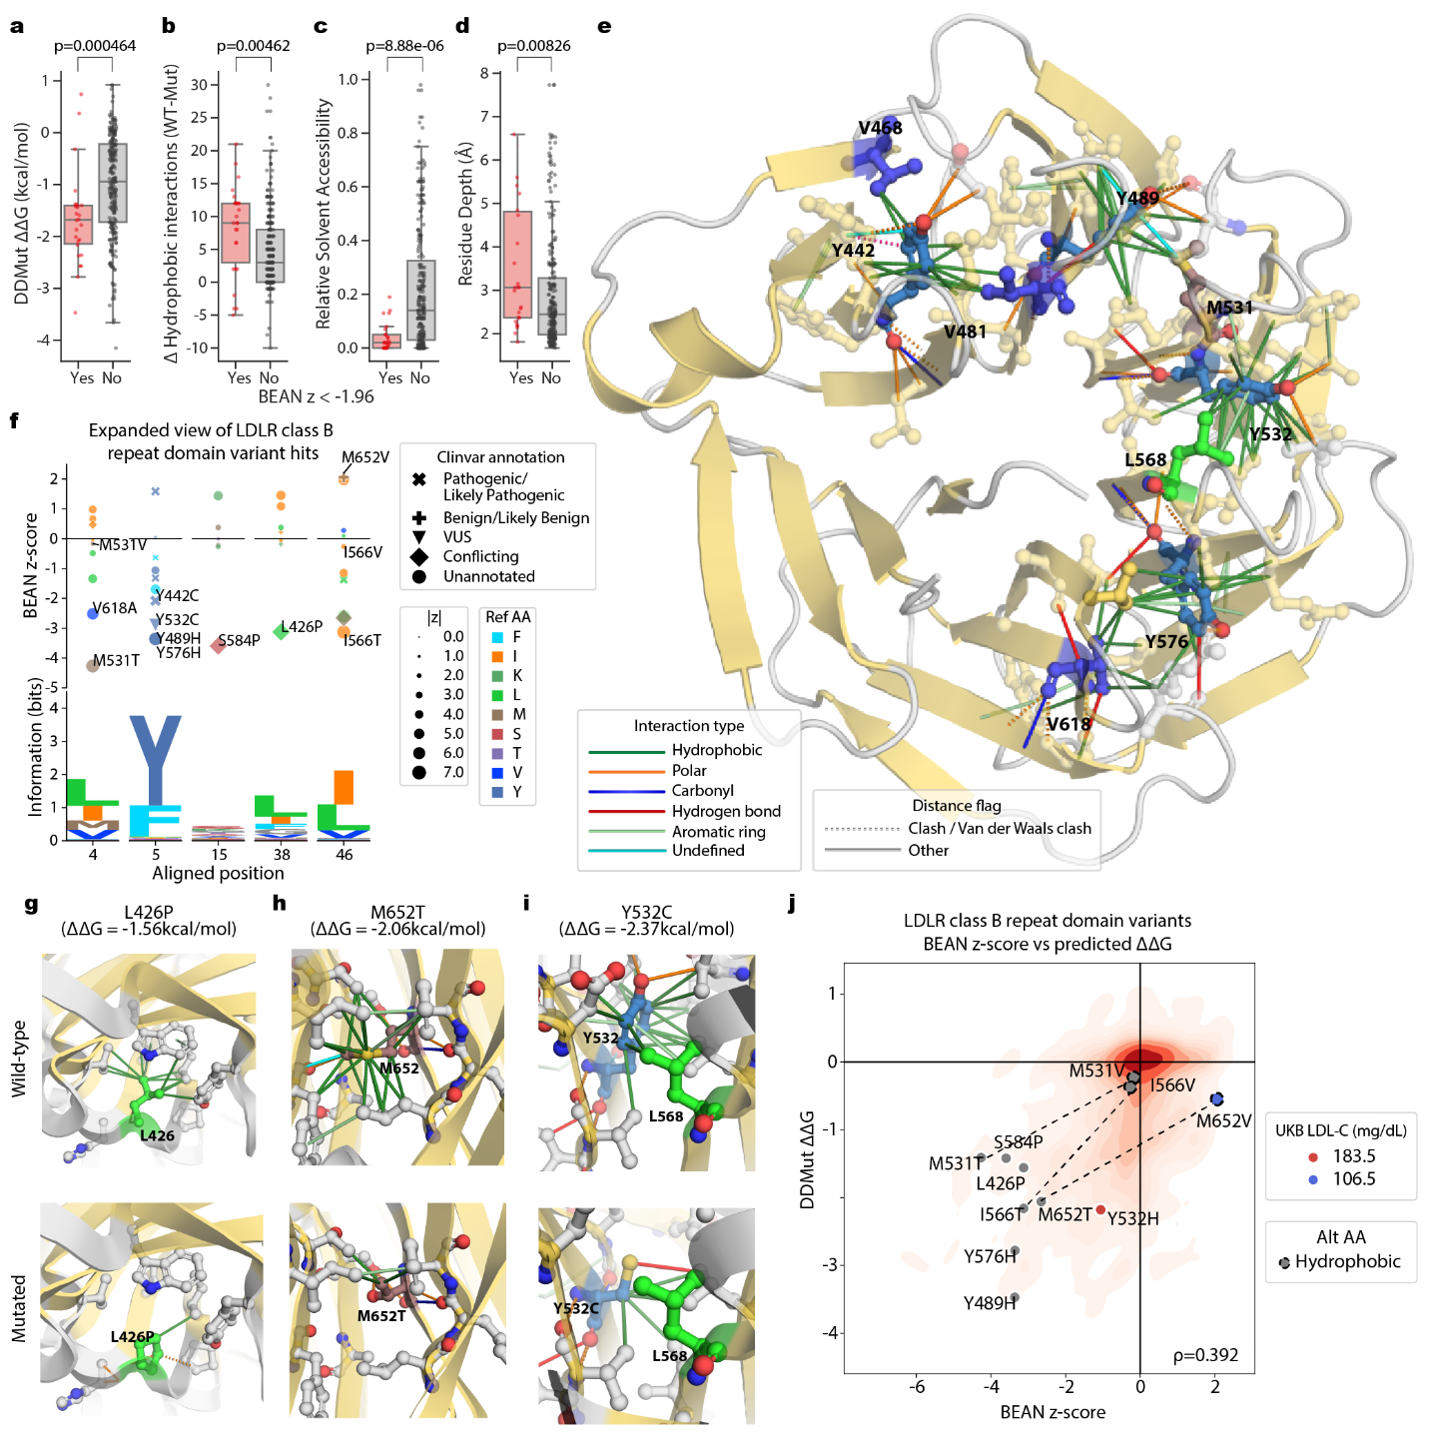
\includegraphics[width=\textwidth]{figures/crisprbean13.png}
	\caption[Deleterious variants in LDLR class B repeats weaken hydrophobic interactions]{\textbf{Deleterious variants in LDLR class B repeats weaken hydrophobic interactions (A)-(D)} Boxplots of 26 significant ($z$ < -1.96) and the rest of 259 variants observed in LDLR class B repeats. $P$-values of two-sided Wilcoxon rank-sum test are denoted. WT; wild-type, Mut; mutated. \textbf{(E)} Conserved interactions involving tyrosine of which mutation showed significant BEAN scores. Simplified interaction types and distance flags as annotated by Arpeggio are shown in the legend. \textbf{(E)} BEAN $z$-scores of positions with conserved hydrophobic residues are shown along with the LDLR class B repeat PFAM HMM logo. \textbf{(G)-(I)} Local atomic interaction in wild-type and mutated structure for ClinVar conflicting variants or VUS L426P, M652T, and Y532C. Residues in the variant positions are colored by the reference amino acids. Residues that interact with the variant position are shown. Variant position and interacting residues are colored by elements (O: red, N: blue, S: yellow). \textbf{(J)} Contour plot of BEAN z-score against $\Delta\Delta$G predicted by DDMut for 872 missense variants. Positions with distinct observed missense variants that disrupt and conserve hydrophobic sidechains are connected by dashed line.}
	\label{fig:crisprbean13}
\end{figure} 
We noticed that an appreciable number of deleterious variants that lack ClinVar pathogenic designation reside in the six LDLR class B repeats. The LDLR class B repeats, also known as YWTD repeats, form a propeller-like structure involved in the release of LDL following its endocytosis. To gain insights into unannotated variant impact, focusing on the LDLR class B repeats, we used the full wild-type LDLR structure from the AlphaFold Protein Structure Database \citep{jumper2021highly, varadi2022alphafold} and the MODELLER \citep{webb2016comparative} -generated mutant structures to calculate changes in interatomic interactions using Arpeggio \citep{jubb2017arpeggio}. Additionally, we predicted the effects of variants on protein stability ($\Delta\Delta$G, negative value indicates destabilization) with DDMut \citep{zhou2023ddmut}. We found that the 26 significant LDLR class B variants induce more destabilizing effects, disrupt more hydrophobic interactions, have lower relative solvent accessibility \citep{rose1985hydrophobicity} (0.041 of maximum residue solvent accessibility), and have higher wild-type residue depth as compared to the other observed variants in this region (\textbf{Fig. \ref{fig:crisprbean13}(A)-(D)}). Collectively, these observations strongly indicate that these significant LDLR class B repeat variants are predominantly buried within the protein core where they engage in extensive hydrophobic interactions essential for protein folding. Moreover, we found a conserved interaction across repeat domains in which a tyrosine holds neighboring propeller blades together through interactions with a hydrophobic residue of the neighboring repeat (\textbf{Fig. \ref{fig:crisprbean13}(E)-(F)}. 

We identified five of these variant pairs (Y442C with V481A, Y442C with V468A, Y489H with M531T, Y532C with L568P, and Y576H with V618A), where all nine positions have at least one variant that weakens their hydrophobic interaction and has a significant BEAN $z$-score. Among the top-ranked unannotated or ClinVar VUS and conflicting variants within LDLR class B repeats, the six most significant variants (L426P, Y489H, M531T, I566T, S584P, and Y576H) all disrupt residues that hold the propeller blades together through hydrophobic interactions (\textbf{Fig. \ref{fig:crisprbean13}(G)-(I)}). Further supporting the importance of hydrophobic interactions, the base editing screen installed additional missense variants at positions 531, 566, and 652 that conserve hydrophobicity. In all cases, mutation into hydrophobic residues has less severe impact from the base editing screen and DDMut-predicted destabilization than mutation into non-hydrophobic residues (\textbf{Fig. \ref{fig:crisprbean13}(J)}). For example, while we find M652T to be highly deleterious (BEAN $z$=-2.65), we find no functional disruption from the hydrophobicity-conserving M652V variant (BEAN $z$=+2.06). This analysis is supported clinically, as M652V is designated in ClinVar as “Likely Benign,” and the average UKB carrier LDL-C is below average (106mg/dL). In summary, structural analysis of rare LDLR variants identified by BEAN provides a basis for the missense variant impact through affecting structural integrity of LDLR, highlighting a central role for hydrophobic interactions that hold together adjacent beta blades of the LDLR class B repeat domain


% ------ Appendix A
\appendix
\chapter{Bioinformatics File Formats}\label{appendix:fileformats}
This appendix describes the bioinformatics- and computational biology-related file formats encountered throughout the manuscript. The descriptions list the major details of each format, providing some context when possible. 

% ----- FASTA file format
\section{FASTA file format}\label{section:fasta-format}
The FASTA file format is a widely used text-based format to represent nucleotide or protein sequences. It typically consists of two parts: a single-line description (header), beginning with ``>'', followed by the sequence data. The header line contains a brief description of the sequence and
may include additional information, such as the sequence ID, source organism, or any relevant annotations. The sequence data comprises the nucleotide (\texttt{A}, \texttt{T}, \texttt{C}, \texttt{G}, \texttt{U}) or amino acid (protein) sequence. The sequence may be arranged as a single line or broken into multiple lines (each 80 bp long) for better readability. FASTA files may contain a single sequence or multiple sequences, with each sequence following the same two-part structure. There is no standard filename extension for FASTA files. Among the most common file extensions there are: \texttt{fasta} and \texttt{fa}.

% ----- FASTQ file format
\section{FASTQ file format}\label{section:fastq-format}
The FASTQ format is a text-based representation designed to store both a biological sequence, typically a nucleotide sequence, and its corresponding quality scores. Each sequence letter and quality score is encoded using a single ASCII character to ensure brevity. Originally created at the Wellcome Trust Sanger Institute with the purpose of bundling a FASTA-formatted (\textbf{Appendix \ref{section:fasta-format}}) sequence and its quality data, the FASTQ format has evolved into the prevailing standard for archiving the results produced by high-throughput sequencing instruments. There is no standard file extension for FASTQ files. However, \texttt{.fq} and \texttt{.fastq} are commonly used file extensions.

% ----- SAM file format
\section{SAM file format}\label{section:sam-format}
The Sequence Alignment Map (SAM) \citep{li2009sequence} is a text-based format developed to store biological sequences aligned to a reference sequence. SAM files present a TAB-delimited structure. The SAM files comprise a header and an alignment section.  The header section, when present, precedes the alignment section. Headers are denoted by ``@''. The alignment section is characterized by 11 mandatory fields and may include a variable number of optional fields (\textbf{Table \ref{tab:sam-file}}). SAM files can be manipulated and examined using SAMtools \citep{li2009sequence}.
The SAM format has become widely adopted for storing diverse data, including nucleotide sequences, generated by next-generation sequencing technologies. The standard has been expanded to accommodate unmapped sequences, and it supports both short and long reads (up to 128 Mbp). SAM is used to store and process mapped data by several tools, such as the Genome Analysis Toolkit (GATK) \citep{mckenna2010genome} or strelka \citep{kim2018strelka2}, and organizations, such as the ENCODE project \citep{encode2012integrated} or 1000 Genomes Project \citep{10002015global}.

% - table: SAM file format fields
\begin{table}[!]
    \centering
    \resizebox{\columnwidth}{!}{%
    \begin{tabular}{|l|l|l|}
        \hline
        \textbf{Field} & \textbf{Type} & \textbf{Description}                   \\ \hline
        QNAME          & string        & Query name                             \\ \hline
        FLAG           & int           & bitwise FLAG                           \\ \hline
        RNAME          & string        & Reference sequence name                \\ \hline
        POS            & int           & Mapping position (1-based)             \\ \hline
        MAPQ           & int           & Mapping quality                        \\ \hline
        CIGAR          & string        & CIGAR string                           \\ \hline
        RNEXT          & string        & Reference name of the mapped/next read \\ \hline
        PNEXT          & int           & Position of the mapped/next read       \\ \hline
        TLEN           & int           & Template length                        \\ \hline
        SEQ            & string        & Read sequence                          \\ \hline
        QUAL           & string        & ASCII Phred-scaled base quality (+ 33) \\ \hline
    \end{tabular}%
    }
    \caption[SAM file format fields]{\textbf{SAM file format fields.} Description of SAM format fields}
    \label{tab:sam-file}
\end{table}

% ----- BAM file format
\section{BAM file format}\label{section:bam-format}
BAM (Binary Alignment Map) \citep{barnett2011bamtools} represents the compressed binary counterpart of the SAM format (\textbf{Appendix \ref{section:sam-format}}). BAM files provide a condensed and indexable representation of nucleotide sequence alignments. SAM/BAM are widely employed by numerous next-generation sequencing and analysis tools. In terms of custom track display, indexed BAM offers a notable advantage over other human-readable alignment formats. This approach enables the processing of alignments from large files that might otherwise cause issues when attempting to analyze the entire files.

% ----- CRAM file format
\section{CRAM file format}\label{section:cram-format}
While BAM (\textbf{Appendix \ref{section:bam-format}}) files encompass all sequence data within a single file, CRAM files achieve a smaller size by leveraging an external ``reference sequence'' file, which is essential for both compression and decompression of the read information. Due to their higher compression density, many organizations and tools are transitioning to the CRAM format to optimize disk space utilization. The work properly, CRAM files necessitate an associated index file, similarly to BAM files.

% ----- BED file format
\section{BED file format}\label{section:bed-format}
The BED (Browser Extensible Data) file format serves as a versatile method to display genomic features on genome browsers, such as the UCSC Genome Browser \citep{lee2020ucsc}. BED files are plain text documents consisting of twelve tab-separated fields, with the first three being mandatory. BED files can be analyzed and processed using various tools, including BEDtools \citep{quinlan2010bedtools}. Currently, there exist several variations of the BED file format. Due to its adaptability, BED files have been extensively employed to summarize diverse genomic features, especially ChIP-seq peak regions. The ENCODE Project provides ChIP-seq peak data in the ENCODE BED \texttt{narrowPeak} format, deviating from the classical BED file format. The ENCODE \texttt{narrowPeak} consists of 10 fields (\textbf{Table \ref{tab:encode-bed}}). This format requires all ten fields to contain values. If data are not available for a certain field, the format defines null values to insert (\textbf{Table \ref{tab:encode-bed}}). Importantly BED \texttt{narrowPeak} files store statistical significance for the called peak, incorporating two fields to store both a $P$-value and a $q$-value.

% - table: ENCODE BED narrowPeak file format fields
\begin{table}[!]
    \centering
    \resizebox{\columnwidth}{!}{%
    \begin{tabular}{|l|l|l|}
        \hline
        \textbf{Field} &
          \textbf{Description} &
          \textbf{Type} \\ \hline
        chrom &
          Name of the chromosome (or contig, scaffold, etc.) &
          mandatory \\ \hline
        chromStart &
          \begin{tabular}[c]{@{}l@{}}Starting position of the feature in the chromosome.\\ The first base in a chromosome is numbered 0\end{tabular} &
          mandatory \\ \hline
        chromEnd &
          \begin{tabular}[c]{@{}l@{}}Ending position of the feature in the chromosome.\\ The chromEnd base is not displayed\end{tabular} &
          mandatory \\ \hline
        name &
          Feature name (preferably unique) &
          optional \\ \hline
        score &
          \begin{tabular}[c]{@{}l@{}}Indicates feature's gray shade to be displayed in the \\ genome browser (0-1000).\end{tabular} &
          optional \\ \hline
        strand &
          \begin{tabular}[c]{@{}l@{}}+/- denote feature's strand or orientation \\ (whenever applicable)\end{tabular} &
          optional \\ \hline
        signalValue &
          \begin{tabular}[c]{@{}l@{}}Measurement of overall (usually, average) \\ enrichment for the region\end{tabular} &
          optional \\ \hline
        pValue &
          \begin{tabular}[c]{@{}l@{}}Feature's statistical significance (-log10). Use -1 \\ if no pValue is assigned\end{tabular} &
          optional \\ \hline
        qValue &
          \begin{tabular}[c]{@{}l@{}}Feature's statistical significance using false\\ discovery rate (-log10). Use -1 if no qValue is \\ assigned\end{tabular} &
          optional \\ \hline
        peak &
          \begin{tabular}[c]{@{}l@{}}Feature's peak summit position (0-based offset from \\ chromStart). Use -1 if no peak summit called\end{tabular} &
           optional \\ \hline
    \end{tabular}%
    }
    \caption[ENCODE BED narrowPeak file format fields]{\textbf{ENCODE BED narrowPeak file format fields.} Description of ENCODE BED narrowPeak format fields.}
    \label{tab:encode-bed}
\end{table}

% ----- MEME file format
\section{MEME file format}\label{section:meme-format}
The MEME file format \citep{bailey2009meme} is a text representation for DNA or amino acid motifs, encoded as PWMs. Several motif discovery tools return motifs in MEME format, in particular those within the MEME suite \citep{bailey2009meme}. As the format is plain text (ASCII), it can be manually crafted using a simple text editor or word processor. A single MEME file can encompass one or more motifs and, if needed, specify the alphabet upon which the motifs are constructed, background frequencies of the alphabet letters, and strand information when dealing with DNA motifs. MEME files comprise five sections: (i) the version line, (ii) alphabet, (iii) strands (optional), (iv) background frequencies, and (v) motifs. The version line denotes the version of the tool (if part of the MEME suite) that produced the motif. The alphabet line includes the motif sequence alphabet, such as \texttt{ACGT} for DNA, \texttt{ACGU} for RNA, and \texttt{ACDEFGHIKLMNPQRSTVWY} for protein sequences. The strands line indicates whether the motif has been discovered using both the forward and reverse strands. The background frequency line provides the letter frequencies of the motif alphabet in the input sequences. These frequencies must sum to 1. The motif section is further divided into three subsections: motif name, motif letter-probability matrix lines, and motif URL (optional). The motif name line contains the motif ID and its full name. This line marks the beginning of a new motif if the file contains more than one motif. The motif letter-probability matrix lines displays a probability table where rows represent motif positions and columns correspond to motif alphabet letters, sorted alphabetically. For a DNA motif, the columns contain A data in the first column, C data in the second, G data in the third, and T data in the fourth. Following the "letter-probability matrix" line, four optional values describe the motif alphabet length, motif width, number of source sites, and source $E$-value. The motif URL section includes a link to the source page for the current motif.

% ----- JASPAR file format
\section{JASPAR file format}\label{section:jaspar-format}
The JASPAR file format \citep{sandelin2004jaspar} features a header line introduced by ``>'', similar to FASTA file headers, followed by the motif ID. In JASPAR motif files there are four lines, each one dedicated to a specific nucleotide (\texttt{A}, \texttt{C},\texttt{G}, \texttt{T}). In JASPAR motif files columns represent motif positions, and rows represent the motif alphabet letters. Each line begins with the corresponding nucleotide, and the subsequent tab-separated raw count values are enclosed in square brackets "[ ]".

% ----- PFM file format
\section{PFM file format}\label{section:pfm-format}
The PFM file format includes a header line introduced by ``>'' and followed by the unique motif identifier. In PFM files rows represent nucleotides, and columns motif positions. Each nucleotide's raw count values are outlined on a separate line, with the row letters ordered alphabetically.


% ------ Appendix B
\chapter{Motif discovery algorithms}\label{appendix:motifdiscovery}
% put some intro

% ----- Algorithmic details of motif discovery software
\section{Algorithmic details of motif discovery software}\label{section:algorithms-motif-appendix}

% ---- Enumerative methods
\subsection{Enumerative methods}\label{subsection:enumerative-methods-appendix}
Enumerative methods for motif discovery aim to identify overrepresented sequence patterns in the input dataset $S$ compared to a background set of sequences $B$. These methods involve counting the approximate occurrences of all possible $4^{k}$ $k$-mers (assuming an alphabet $\Sigma={A,C,G,T}$) in $S$ and assessing the statistical significance of the difference between the observed matches in $S$ and $B$ or the expected match frequencies based on a background model (\textbf{Section 4.2.2}). The table in \textbf{Appendix \ref{appendix:motifdiscovery}.2} provides a summary of the key characteristics of enumerative methods. Early approaches employed heuristics to explore the motif search space, allowing for mismatching positions. However, more recent methods such as Weeder \citep{pavesi2001algorithm,pavesi2004weeder} and SMILE \citep{marsan2000algorithms} present more efficient and accurate strategies by utilizing suffix trees (STs) to index the input sequences. Both Weeder and SMILE leverage STs for efficient approximate pattern matching, searching all $k$-mers occurrences in $S$ while allowing mismatches at any motif position. Although Weeder and SMILE share a similar data structure, they differ in their approaches to assess the significance of the identified motifs. SMILE evaluates motif significance by comparing the number of occurrences of a specific motif in $S$ with its expected frequency in $B$. To estimate expected occurrences, SMILE either generates a random set of sequences using a Markov model or uses a negative set of sequences that do not contain instances of the target binding sites. On the other hand, Weeder compares the observed occurrences of each motif candidate with its expected frequencies derived from the regulatory regions of the same organism as the input sequences. It is important to note that both SMILE and Weeder may require several hours to complete on datasets consisting of thousands of sequences generated by high-throughput assays. To address this challenge, there has been a growing interest in the development of enumerative motif discovery methods capable of efficiently analyzing large datasets comprising thousands of sequences. MDscan \citep{liu2002algorithm} uses word enumeration for motif discovery in sequence datasets. Initially designed for ChIP-on-Chip datasets, MDscan identifies non-redundant patterns that are abundant in the most enriched ChIP peak sequences, rather than enumerating all possible words from $s \in S$. To assess the statistical significance of motif candidates, MDscan employs a third-order Markov model as background. Amadeus \citep{linhart2008transcription} evaluates all $k$-mers in input sequence datasets. Amadeus has been originally designed to focus on datasets generated by ChIP-on-Chip assays. It groups similar sequence patterns into lists and combines these lists into motifs, which are statistically evaluated using a hypergeometric test to determine their significance. Recently, both MDscan and Amadeus have been extended to support other high-throughput sequencing technologies such as ChIP-seq and DNase-seq. Additionally, Amadeus has been adapted to analyze data from multiple organisms, aiming to identify conserved motifs across species. Enumerating words in datasets containing thousands of sequences can be computationally expensive in most scenarios. DREME \citep{bailey2011dreme} presents an alternative approach using regular expressions to enhance motif discovery on large sequence datasets. DREME leverages regular expressions for counting approximate motif occurrences in both $S$ and $B$, allowing a more efficient exploration of the motif search space across extensive sequence sets. DREME generates the background dataset from $S$ using a Markov model or utilizes a user-provided negative set of sequences. To assess the statistical significance of the discovered motifs, DREME employs Fisher’s exact test, comparing the occurrences of motifs in sequences from $S$ and $B$. However, regular expressions for motif discovery hide certain drawbacks: they (i) can be computationally demanding on large datasets, (ii) might identify patterns as motifs that are not biologically relevant, and (iii) may not capture all variations of a motif. While enumerative methods employing STs may address some of these challenges, they are computationally demanding and often lack scalability when analyzing thousands of sequences. Trawler, HOMER, and STREME \citep{ettwiller2007trawler,heinz2010simple,bailey2021streme} propose different enhancements for discovering motifs using STs in the context of large-scale sequence datasets. Trawler \citep{ettwiller2007trawler} focuses on detecting transcription factor binding site (TFBS) motifs in extensive datasets like ChIP-seq and DNase-seq data. Employing suffix trees, Trawler enumerates all sequence patterns in both $S$ and $B$, measuring their frequencies to identify overrepresented motifs in $S$. Trawler allows for mismatching positions by employing degenerate consensuses when matching motif sequences. Statistical evaluation of prioritized patterns in Trawler involves $z$-scores derived from the normal approximation to the binomial distribution. This approach facilitates fast computation without the need to correct for the effect of overlapping motifs. Trawler constructs motifs by clustering similar and significant patterns. HOMER \citep{heinz2010simple}, tailored to analyze ChIP-seq datasets, indexes both the input and background sequence datasets using STs. It searches for overrepresented patterns in the target sequences through approximate pattern matching on the ST. The identified overrepresented $k$-mers are clustered into motif candidates, which are statistically evaluated using either the hypergeometric or binomial test. By avoiding explicit counting of $k$-mer frequencies, HOMER reduces its running time. The significant motif candidates undergo further refinement by eliminating those lacking conserved positions or exhibiting low information content. While originally designed for ChIP-seq, HOMER demonstrates applicability to sequence datasets from diverse assays. STREME \citep{bailey2021streme} proposes a strategy to enhance motif discovery efficiency by employing approximate matching on suffix trees. STREME constructs an ST from $S$ and identifies overrepresented seed words of different lengths through exact matching on the ST. Statistical significance of each seed word is assessed using either the Fisher’s exact test or binomial distribution. STREME then counts the number of approximate matches for the most significant words on the ST, using a mismatch threshold. Subsequently, STREME prioritizes and groups the most significant seed words to derive the corresponding motifs. This approach enables STREME to identify motifs of different lengths in a single tree visit, substantially reducing the running time for motif discovery.

% ---- Alignment-based methods
\subsection{Alignment-based methods}\label{subsection:alignment-methods-appendix}
Alignment-based motif discovery algorithms utilize employ alignment profiles to identify potential TFBS within the input sequence dataset $S$. These algorithms construct profiles by combining potential motif instances and then assess each profile's score using various statistical measures. However, the exhaustive enumeration of all possible alignments is impractical. As a result, efforts have been directed towards incorporating heuristics to efficiently generate high-quality alignments. The Table in \textbf{Appendix \ref{appendix:motifdiscovery}.2} provides a summary of the key characteristics of the alignment-based methods discussed in this section. CONSENSUS \citep{hertz1999identifying} uses a greedy algorithm to identify TFBS alignment profiles. It assumes a single occurrence of the motif in each sequence of $S$. Assuming $|M|=k$, CONSENSUS starts by comparing all $k$-mers in two sequences, $s_{1}, s_{2} \in S$, generating a $4 \times k$ profile for each $k$-mer pair. Each profile undergoes individual scoring based on information content, and the alignments with the highest scores are retained. Subsequently, CONSENSUS compares each profile to the $k$-mers of another sequence, $s_{3} \in S/\{s_{1},s_{2}\}$, producing a new set of profiles involving three sequences. These resulting profiles are scored using information content, and the alignments with the highest scores are preserved. CONSENSUS incrementally stores the best partial alignments with the hope of eventually finding the optimal profile. However, in cases where motifs lack conservation, the algorithm may store profiles corresponding to random $k$-mers, potentially excluding highest-scoring alignments. MEME \citep{bailey1994fitting,bailey1995value,bailey2006meme} introduced an EM strategy to comprehensively explore the entire motif search space, distinguishing itself from CONSENSUS by not relying on partial solutions. Initially, MEME initializes a profile with one $k$-mer from each sequence, $s \in S$. This starting profile undergoes iterative refinement through an EM strategy involving two steps: the E-step and the M-step. In the E-step, MEME computes a likelihood score for each $k$-mer in $S$, using the current alignment profile. In the M-step, MEME assigns a weight to each $k$-mer in the current profile, proportional to the scores computed during the E-step, and updates the alignment by replacing low-scoring $k$-mers with others that better fit the current profile. MEME accommodates sequences with zero or more than one motif occurrence, provides background models of different orders, and assigns a $P$-value to each identified motif. This $P$-value indicates the probability of obtaining a profile with the same information content by chance, offering a measure of confidence for each discovered motif. Algorithms employing Gibbs sampling address MEME’s main limitation of potentially converging to local maxima, thus not always reporting the best alignment profile. The generic Gibbs sampling algorithm begins by initializing a profile with $k$-mers randomly chosen from each sequence in the input dataset $S$. In each iteration, the algorithm removes a $k$-mer from the profile originating from a specific sequence $s$ and computes a likelihood score for each $k$-mer in $s$ based on the modified profile. This score reflects how well each $k$-mer fits the profile, rather than a background model, akin to MEME. Subsequently, the algorithm replaces the removed $k$-mer with a new one chosen with a probability proportional to its likelihood score. This process repeats until a fixed number of iterations or until no further changes to the profile occur. The foundational Gibbs sampling algorithm \citep{lawrence1990expectation} assumes that each sequence in $S$ contains precisely one binding site. Motif sampler \citep{neuwald1995gibbs} extended the original algorithm to accommodate sequences containing one, multiple, or no binding sites. However, it necessitates the user to provide an estimate of the expected number of occurrences of the TFBS in the input sequence dataset. Further modifications to the Gibbs sampling procedure were introduced by AlignACE \citep{hughes2000computational} and ANN-spec \citep{workman1999ann}, enabling the simultaneous exploration of TFBS on both strands. AlignACE also incorporates a sampling method that considers the relative position of each $k$-mer within a group in relation to gene transcription start sites (TSS). This ensures that functional motifs correspond to similar regions occurring at comparable distances from the TSS. ANN-spec couples Gibbs sampling with a perceptron artificial neural network, replacing the alignment profile. Bioprospector \citep{liu2000bioprospector} and MotifSampler \citep{thijs2001higher} suggest using a third-order Markov model as a background, enhancing the predictive performance of the Gibbs sampling algorithm. Typically, alignment-based motif discovery methods assume that the motif length is known \emph{a priori}. GLAM \citep{frith2004finding} modified the Gibbs sampling procedure to estimate the optimal alignment length and employed simulated annealing to optimize the motif profiles. GLAM was further extended to consider gapped motifs, introducing flexibility to motif variability \citep{frith2008discovering}. While these methods employ heuristics for efficiently exploring the motif solution space, they were initially designed to analyze datasets comprising hundreds or a few thousand sequences. To address this limitation, developers of motif discovery algorithms have proposed novel alignment-based methods extending the original ideas to analyze the large datasets generated by NGS assays. MEME-ChIP \citep{machanick2011meme} extends the original MEME algorithm to handle large ChIP datasets. Rather than analyzing the entire input dataset, MEME-ChIP runs the EM motif search on a random subset of sequences from $S$. Additionally, MEME-ChIP prioritizes motifs discovered around ChIP-seq peak summits. While originally designed for ChIP-seq and ChIP-on-Chip datasets, MEME-ChIP is versatile enough to be applied to datasets generated by different experimental assays. Similarly, STEME \citep{reid2011steme} enhances the MEME algorithm by indexing the input sequences using a suffix tree (ST). Employing a branch-and-bound strategy on the ST, STEME avoids evaluating the likelihood of all possible $k$-mers during MEME's E-step. ChIPMunk \citep{kulakovskiy2010deep} introduces an efficient method for discovering motifs in thousands of genomic sequences. In contrast to traditional approaches using EM, ChIPMunk prioritizes a set of enriched $k$-mers initially and constructs a profile from them. Subsequently, the profile undergoes a scalable EM-like refinement to maximize the discrete information content \citep{kulakovskiy2009discovery}. Moreover, ChIPMunk leverages ChIP peak shapes to weight the contribution of each sequence $s \in S$ to the motif definition, enhancing the accuracy of identified motifs. XXmotif \citep{hartmann2013p} integrates enumerative motif discovery with profile refinement. It iteratively selects sets of $k$-mers from $S$ to maximize their fitness to the profile and enhances the motif's fitness to $S$. Similarly, ProSampler \citep{li2019prosampler} proposes a highly optimized and ultra-fast hybrid method for discovering motifs in ChIP-seq datasets. It combines motif enumeration with Gibbs sampling to refine motif profiles effectively.

% ---- Probabilistic graphical models-based methods
\subsection{Probabilistic graphical models-based methods}\label{subsection:probabilistic-methods-appendix}
Whether including dependencies between neighboring and non-neighboring nucleotides in TFBS motif discovery and models has been a longstanding topic of discussion within the research community. The Table in \textbf{Appendix \ref{appendix:motifdiscovery}.2} provides a concise overview of the key characteristics of probabilistic graphical models-based methods covered in this section. Motif discovery algorithms, such as Dimont \citep{grau2013general} and diChIPMunk \citep{kulakovskiy2013binding}, have been developed to detect and represent TFBS motifs using DWMs. These methods, employing more sophisticated approaches than PWMs, demonstrate scalability to large datasets comprising thousands of sequences without compromising accuracy. In the case of Dimont \citep{grau2013general}, the initial motif profile is initialized by combining the most overrepresented and non-redundant $7$-mers in sequence set $S$, forming an alignment of length $|M|$. Dimont assigns higher weights to the positions at the center of the profile. To ensure scalability with large datasets, Dimont uses a highly optimized supervised posterior probabilities estimation technique to refine the initial profile. The algorithm also filters redundant and reverse complement motifs that match the highest-scoring profiles, contributing to a reduction in runtime. Finally, the motif profiles undergo optimization using Kullback-Leibler divergence. Similarly, diChIPMunk \citep{kulakovskiy2013binding} extends the original ChIPMunk \citep{kulakovskiy2010deep} procedure to construct DWMs, by considering motif dinucleotide frequencies. The algorithm employs an EM-like approach to optimize the starting motifs and weighs the contribution of sequences to the TFBS motif, accounting for the ChIP peak shape. Unlike ChIPMunk, which maximizes the discrete information content on individual nucleotides, diChIPMunk optimizes this measure based on dinucleotide frequencies. TFFMs \citep{mathelier2013next} introduces a model based on hidden Markov models (HMMs) to capture dinucleotide dependencies between neighboring TFBS positions and learn the properties of sequences flanking the binding sites. By incorporating insertion and deletion states into the model, TFFMs can accommodate variable motif lengths, making it a flexible model. TFFMs leverage the MEME algorithm \citep{bailey1994fitting,bailey1995value,bailey2006meme} to identify motif candidates, subsequently used to train the HMMs employing the Baum-Welch algorithm. Similarly, Discrover \citep{maaskola2014binding} proposes a discriminative approach for motif discovery in ChIP-seq datasets, using HMMs. Initially, Discrover identifies overrepresented motifs in the input dataset $S$ using regular expressions, similar to DREME \citep{bailey2011dreme}. The identified motif candidates serve as seeds to initialize an HMM. The algorithm prioritizes these candidates based on different objective functions \citep{maaskola2014binding}, such as likelihood or mutual information, to select the most promising seeds. Subsequently, the initial HMM undergoes refinement through iterative gradient optimization of the model likelihood. Markov Models (MMs) and HMMs can be extended to incorporate variable-order dependencies between neighboring and non-neighboring motif positions, akin to Bayesian Networks (BNs). Slim \citep{keilwagen2015varying} introduces a framework for learning dependencies of different orders between neighboring and non-neighboring nucleotides. The dependency orders are pruned in a data-driven manner, iteratively establishing the motif positions on which each nucleotide depends. The models are trained using motif candidates prioritized by running Dimont on $S$, maintaining scalability on large sequence datasets. However, to ensure scalability on large datasets, methods like HMMs and MMs often learn low-order dependencies from the input sequences. Addressing this, BaMMotif \citep{siebert2016bayesian,ge2021bayesian} presents an efficient motif discovery algorithm that learns high-order dependencies (up to the 5-th order) on thousands of sequences using an optimized Bayesian approach to train MMs. To prevent model overfitting, the algorithm uses the conditional probabilities of $(q-1)$-th order as priors for the $q$-th order conditional probabilities during training. The algorithm iteratively optimizes the model parameters until convergence through Expectation-Maximization (EM). During the E-step, BaMMotif estimates the probability that each position of each $s \in S$ is a motif starting position, using the current model. In the M-step, the algorithm refines the model using the motif candidates identified in the previous step. The algorithm dynamically adapts the model parameters during training to capture variable orders of dependencies.

% ---- SVM-based methods
\subsection{SVM-based methods}\label{subsection:svm-methods-appendix}
Support Vector Machines (SVMs) offer an efficient and scalable approach for learning complex sequence features in different biological contexts, including TFBS. SVMs have demonstrated scalability, even when dealing with thousands of sequences typical of datasets generated by high-throughput protocols. Notably, SVMs not only capture the motif itself but also incorporate other sequence features surrounding the binding sites into the learned model. A summarized overview of the key features of SVM-based methods discussed in this section can be found in the Table in \textbf{Appendix \ref{appendix:motifdiscovery}.2}. Kmer-SVM \citep{lee2011discriminative,fletez2013kmer} proposes a scalable framework using SVMs for the discovery and representation of TFBS as SVM models. The algorithm operates on a foreground dataset $S$ and a background dataset $B$. It dissects the input sequences $s \in S$ into contiguous $k$-mers (with $k \sim 10$ base pairs) and computes their frequencies in both datasets. Employing a trie \citep{bodon2003trie} for indexing $S$ and $B$, Kmer-SVM achieves linear runtime. The complete frequency profiles of $k$-mers within each sequence are stored as feature vectors, serving as input for training the SVM kernel. Kmer-SVM employs the spectrum kernel, optimizing parameters to effectively distinguish between positive and negative sequences (support vectors). Additionally, Kmer-SVM offers a weighted version of the spectrum kernel, where the contributions of k-mers are weighted based on their positional information within the sequence. However, this implementation lacks flexibility in $k$-mer frequency estimation and encounters scalability issues when analyzing datasets comprising tens of thousands of sequences containing degenerate and long ($>10$ base pairs) motifs. \cite{agius2010high} present a more flexible framework through the training of Support Vector Regression models (SVRs). The algorithm proposes the usage of a dinucleotide mismatch kernel (di-mismatch kernel). While the basic mismatch kernel permits up to $m$ mismatches in each $k$-mer match, for small $m$ values, the mismatch neighborhood of a given $k$-mer becomes excessively large. To address this issue, the authors introduced the di-mismatch kernel, which tallies mismatching nucleotides and favors $k$-mers with consecutive mismatches. Furthermore, the kernel is tailored for sets of unique $k$-mers occurring in training sequences, such as PBM probe sequences. Nevertheless, this method is constrained by considering short $k$, restricting the ability to discover longer motifs. To overcome this limitation, gapped-$k$-mers \citep{ghandi2014robust} introduce gaps in non-informative motif positions to accommodate longer motifs while preserving scalability on large datasets. A gapped-$k$-mer is defined by a pair of values ($l$, $k$) representing the full length and the number of non-gap positions, respectively. For example, \texttt{A*CG} is a gapped-$k$-mer with $l=4$ and $k=3$. Gkm-SVM \citep{ghandi2014enhanced,ghandi2016gkmsvm} constructs feature vectors for each input sequence by tallying the occurrences of gapped-$k$-mers in both positive and negative datasets, as opposed to exact $k$-mer frequencies. These feature vectors are then used to train the gapped-$k$-mer kernel, which computes support vectors to distinguish between bound and unbound sequences. To determine the SVM hyperplane, the feature vectors for each sequence are mapped to the normalized counts of their distinct gapped-$k$-mers. However, this approach has been shown to be non-scalable when applied to large sequence datasets ($> 10,000$ sequences). LS-GKM \citep{lee2016ls} enhances Gkm-SVM to effectively handle large-scale datasets. Additionally, LS-GKM introduces a weighted version of the gapped-$k$-mer kernel, along with the \textbf{gkmrbf} kernel and its weighted counterpart, to capture non-linear relationships between sequence features.

% ---- Deep Neural Networks-based methods
\subsection{Deep Neural Networks-based methods}\label{subsection:dnn-methods-appendix}
Deep neural networks (DNNs) have demonstrated considerable success in addressing various challenges in computational biology, including the discovery and classification of transcription factor binding site motifs. The Table in \textbf{Appendix \ref{appendix:motifdiscovery}.2} provides a concise overview of the key characteristics of DNN-based methods. Convolutional neural networks (CNNs) \citep{lecun2015deep} have found widespread applications in motif discovery. Typically, CNNs designed for motif discovery consist of several fundamental layers \citep{zeng2016convolutional}. In the first layer, known as the convolutional stage, input sequences from the dataset $S$ undergo scanning with a set of convolutional filters (motif kernels). The resulting response values are then forwarded to the subsequent layer, called max-pooling layer. Within the max-pooling layer, maximal responses for each convolutional layer are selected and incorporated into feature vectors. The subsequent layer, the neural network stage, transforms these feature vectors into scalar scores, representing the likelihood of each site containing a TFBS. To mitigate overfitting, a dropout layer is frequently introduced at this stage, randomly masking portions of the neural network output. The output layer typically comprises two fully connected neurons, indicating the model predictions for "bound" or "unbound" sequences. Backpropagation and gradient descent are commonly employed to iteratively estimate and optimize the CNN parameters. One of the pioneering proposals utilizing CNN for motif discovery on ChIP-seq, HT-SELEX, and PBM is DeepBind \citep{alipanahi2015predicting}. The DeepBind architecture introduces two variations to the basic CNN architecture: a rectification layer and the inclusion of averaging and maximization steps in the pooling layer. The rectification layer identifies sequences that align well with the convolutional kernel by shifting the response by some nucleotides and masking poorly matched positions. In the pooling layer, DeepBind calculates both maximum and average kernel responses, allowing for the identification of cumulative effects of short motifs and the determination of the locations of longer TFBS, respectively. To visualize the discovered motifs, DeepBind computes weighted ensembles of PWMs, obtained by aligning the sequences activating the kernels, centered around the position with the maximum response. Basset \citep{kelley2016basset} enhances the basic CNN architecture by incorporating three additional convolutional layers after the pooling stage, followed by two fully connected neural networks. The model's parameters are initialized randomly and subsequently adjusted adaptively through backpropagation. Basset represents the identified motifs using PWMs. BPNet \citep{avsec2021base} introduces further modifications to the CNN architecture to address the limitations observed in methods like DeepBind and Basset. By integrating nine dilated convolutional layers and eliminating the pooling stage, BPNet preserves the spatial and base resolution of the input data, capturing the intricacies of the discovered motifs. In its original implementation, BPNet utilizes ChIP-exo signal intensity values instead of binary labels during model training, enhancing the precision of predictions. BPNet also incorporates multitask learning, enabling the simultaneous discovery of multiple motifs. By integrating control experiment data, BPNet mitigates overfitting and enhances overall model performance. Considering that TF-DNA interactions involve complex long-term and short-term dependencies, recurrent neural networks (RNNs) prove suitable for modeling such intricate relationships. RNNs were initially introduced to model sequential signals exhibiting stationary features over time. Long Short-Term Memory Networks (LSTMs) \citep{hochreiter1997long}, a variant of RNNs, adeptly capture both long-term and short-term dependencies by learning the positional dynamics of sequential signals. Bi-directional long/short-term memory (BLSTMs) networks represent variations of standard LSTMs, amalgamating the outputs of two RNNs—one analyzing sequential data from left to right and the other from right to left (corresponding to the forward and reverse strands in a genomic context). DeeperBind \citep{hassanzadeh2016deeperbind} proposes a hybrid CNN-LSTMs architecture that effectively captures long-term and short-term positional dependencies. DeeperBind omits the pooling layer to prevent the loss of positional information concerning subregions activating the kernels in the convolutional stage. DanQ \citep{quang2016danq} introduces a hybrid architecture by incorporating CNNs and BLSTMs. The BLSTM layer replaces the fully connected neural network, followed by a dense layer of rectified linear units and a multi-task sigmoid output stage. Situating the BLSTM layer between the pooling and the dense rectified stages enables DanQ to capture the positional dynamics of the input sequences. The parameters of DanQ can be initialized with either random values or known motifs. The identified motifs are represented as PWMs, computed by aligning the sequences that activate the kernels. FactorNet \citep{quang2019factornet} extends the DanQ framework by integrating additional features during model training, such as DNase-seq signals. To mitigate overfitting and reduce training complexity, FactorNet employs a Siamese architecture that accounts for the reverse complement. The Siamese architecture employs identical networks sharing weights for both the forward and reverse strands, ensuring consistent outputs and reducing the amount of required training data.

% ----- Catalogue of Motif discovery algorithms and software for discover Transcription Factor Binding sites in DNA sequences
\section{Catalogue of Motif discovery algorithms and software for discover Transcription Factor Binding sites in DNA sequences}\label{section:algorithms-table-appendix}
The table in this section lists the algorithms discussed in \textbf{Section 4.2.2}, and provides information for each algorithm, including associated publications (\textbf{Refs.}), the original data type used for development and testing in the original publication (\textbf{Original input data type}), the motif model returned (\textbf{Output}), theoretical advantages (\textbf{Pros}), drawbacks (\textbf{Cons}), the year of publication (\textbf{Year}), a link to the code or website (\textbf{Availability}), and details on how each software is distributed to the community (\textbf{Availability type}).

% - table: Motif discovery algorithms and software for discover Transcription Factor Binding sites in DNA sequences
\begin{table}[H]
\centering
\resizebox{\textwidth}{!}{%
\begin{tabular}{|l|l|l|l|l|l|l|l|l|l|}
\hline
\textbf{Motif discovery method} & \textbf{Algorithm} & \textbf{Refs.} & \textbf{Original input data type} & \textbf{Output} & \textbf{Pros} & \textbf{Cons} & \textbf{Year} & \textbf{Availability} & \textbf{Availability type} \\ \hline
                       &           &                              &                                                   &        &                             &                             &      &              &                   \\ \hline
                       &           &                              &                                                   &        &                             &                             &      &              &                   \\ \hline
                       &           &                              &                                                   &        &                             &                             &      &              &                   \\ \hline
                       &           &                              &                                                   &        &                             &                             &      &              &                   \\ \hline
                       &           &                              &                                                   &        &                             &                             &      &              &                   \\ \hline
\end{tabular}%
}
\caption[Motif discovery algorithms and software for discover Transcription Factor Binding sites in DNA sequences]{\textbf{Motif discovery algorithms and software for discover Transcription Factor Binding sites in DNA sequences.}}
\label{tab:motif_discovery_algorithms}
\end{table}

% ------  begin bibliography
\bibliography{biblio}
\bibliographystyle{natbib}





\end{document}